\documentclass[11pt]{article}
\usepackage[margin=1in]{geometry}
\usepackage[T1]{fontenc}
\usepackage{lmodern}
\usepackage{microtype}
\usepackage{amsmath,amssymb,amsthm}
\usepackage{booktabs}
\usepackage{array}
\usepackage{tabularx}
\usepackage{longtable}
\usepackage{enumitem}
\usepackage{xcolor}
\usepackage{float}
\usepackage{graphicx}
\usepackage[skip=5pt,font=small]{caption}
\usepackage{pgfplots}
\pgfplotsset{compat=1.18}
\usepgfplotslibrary{groupplots}
\usepackage[colorlinks=true,linkcolor=black,citecolor=black,urlcolor=blue!50!black]{hyperref}
\setlist{itemsep=2pt,topsep=4pt}
\setlength{\emergencystretch}{3em}
\renewcommand{\topfraction}{0.9}
\renewcommand{\bottomfraction}{0.8}
\renewcommand{\floatpagefraction}{0.85}
\renewcommand{\textfraction}{0.08}
\setcounter{tocdepth}{2}
\newtheorem{proposition}{Proposition}
\newtheorem{lemma}{Lemma}
\newtheorem{corollary}{Corollary}
\newcommand{\E}{\mathbb{E}}
\newcommand{\V}{\mathbb{V}}
\newcommand{\Cov}{\mathbb{C}}
\newcommand{\Var}{\operatorname{Var}}
\newcommand{\tr}{\operatorname{tr}}
\newcommand{\diag}{\operatorname{diag}}
\newcommand{\st}{\tilde\sigma}
\newcommand{\op}{\mathrm{op}}
\newcommand{\cR}{\mathcal{R}}
\newcommand{\cG}{\mathcal{G}}
\newcommand{\bnu}{\bar\nu}
\newcommand{\bth}{\bar\vartheta}
\newcommand{\fevc}{\texorpdfstring{\texttt{fevc}}{fevc}}
\newcommand{\code}[1]{\texttt{#1}}
\newcommand{\pend}{\textit{stopped}}
\definecolor{cstay}{HTML}{0072B2}
\definecolor{cmove}{HTML}{D55E00}
\definecolor{cgrey}{HTML}{555555}
\makeatletter
\newcommand{\R}[1]{\ifcsname res@#1\endcsname\csname res@#1\endcsname\else\textbf{[\detokenize{#1}]}\fi}
\newcommand{\setres}[2]{\expandafter\gdef\csname res@#1\endcsname{#2}}
\newcommand{\tabinput}[1]{\@@input #1 }
\makeatother
\setres{real.theta.alpha}{0.0970}
\setres{real.se.alpha}{2.18}
\setres{real.relse.alpha}{0.22\%}
\setres{real.plugin.alpha}{0.1087}
\setres{real.theta.psi}{0.0261}
\setres{real.se.psi}{1.96}
\setres{real.relse.psi}{0.75\%}
\setres{real.plugin.psi}{0.0320}
\setres{real.theta.cov}{0.0134}
\setres{real.se.cov}{0.96}
\setres{real.relse.cov}{0.71\%}
\setres{real.plugin.cov}{0.0085}
\setres{real.theta.sum}{0.1499}
\setres{real.se.sum}{0.95}
\setres{real.relse.sum}{0.06\%}
\setres{real.plugin.sum}{0.1577}
\setres{real.rel_se_sum}{0.06\%}
\setres{real.relse.min}{0.06\%}
\setres{real.relse.max}{0.75\%}
\setres{real.run_maxdiff}{0.6\%}
\setres{real.se_solves}{260}
\setres{real.se_seconds}{131}
\setres{real.factor_minutes}{9}
\setres{real.probe_solves}{4{,}800}
\setres{real.floor.scale}{0.00\%}
\setres{real.floor.profile}{0.00\%}
\setres{real.floor.final}{0.00\%}
\setres{real.load.c0}{-1.12}
\setres{real.load.c1}{2.01}
\setres{real.profile_r2}{0.037}
\setres{real.capped.stayers}{2.5\%}
\setres{real.capped.movers}{1.0\%}
\setres{real.capped.first_term.sum}{26\%}
\setres{real.capped.first_term.max}{26\%}
\setres{real.coef.one}{0.81}
\setres{real.coef.a}{-0.33}
\setres{real.coef.aa}{0.22}
\setres{real.coef.p}{-0.08}
\setres{real.coef.pp}{0.02}
\setres{real.coef.ap}{-0.00}
\setres{real.share.movers.alpha}{97\%}
\setres{real.share.stayers.alpha}{3\%}
\setres{real.first_over_V.alpha}{110\%}
\setres{real.adjust_over_V.alpha}{-0.03\%}
\setres{real.share.movers.psi}{100\%}
\setres{real.share.stayers.psi}{0\%}
\setres{real.first_over_V.psi}{111\%}
\setres{real.adjust_over_V.psi}{0.00\%}
\setres{real.share.movers.cov}{100\%}
\setres{real.share.stayers.cov}{0\%}
\setres{real.first_over_V.cov}{141\%}
\setres{real.adjust_over_V.cov}{0.00\%}
\setres{real.share.movers.sum}{77\%}
\setres{real.share.stayers.sum}{23\%}
\setres{real.first_over_V.sum}{108\%}
\setres{real.adjust_over_V.sum}{-0.18\%}
\setres{real.adjust_max}{0.19\%}
\setres{real.max_stayer_share}{0.5\%}
\setres{real.max_mover_share}{1.9\%}
\setres{real.d2.min}{0.0006}
\setres{real.d2.max}{0.0070}
\setres{real.reff.min}{900}
\setres{real.reff.max}{4{,}600}
\setres{real.lambda.min}{0.0004}
\setres{real.lambda.max}{0.0024}
\setres{real.n.rows}{4{,}063{,}732}
\setres{real.n.mover_rows}{1{,}034{,}376}
\setres{real.n.stayer_rows}{3{,}029{,}356}
\setres{real.n.person_years}{5{,}163{,}428}
\setres{real.n.firms}{86{,}647}
\setres{real.n.workers}{1{,}106{,}419}
\setres{real.n.stayers}{666{,}090}
\setres{real.n.movers}{440{,}329}
\setres{real.share.stayer_rows}{75\%}
\setres{real.share.stayer_py}{59\%}
\setres{real.within_match_mean}{0.013}
\setres{real.stayers_mean}{0.015}
\setres{real.within_match_matches}{560{,}235}
\setres{real.lo.len1}{0.043}
\setres{real.lo.longer.min}{0.055}
\setres{real.lo.longer.max}{0.057}
\setres{real.prof.alpha.stay.lo}{2.68}
\setres{real.prof.alpha.stay.hi}{1.18}
\setres{real.prof.alpha.stay.mid}{0.67}
\setres{real.prof.alpha.fit.lo}{2.25}
\setres{real.prof.alpha.fit.hi}{1.06}
\setres{real.prof.alpha.fit.mid}{0.83}
\setres{real.prof.alpha.move.lo}{2.42}
\setres{real.prof.alpha.move.hi}{1.08}
\setres{real.prof.alpha.move.mid}{0.76}
\setres{real.prof.psi.stay.lo}{1.35}
\setres{real.prof.psi.stay.hi}{0.91}
\setres{real.prof.psi.stay.mid}{0.97}
\setres{real.prof.psi.fit.lo}{1.32}
\setres{real.prof.psi.fit.hi}{0.89}
\setres{real.prof.psi.fit.mid}{0.98}
\setres{real.prof.psi.move.lo}{1.45}
\setres{real.prof.psi.move.hi}{1.12}
\setres{real.prof.psi.move.mid}{0.89}
\setres{dec.N1.gap.max}{14\%}
\setres{dec.N1.fit.maxgap}{17\%}
\setres{dec.N1.fit.bottom}{+13\%}
\setres{dec.N1.fit.mid}{-4\%}
\setres{dec.N1.fit.top}{+17\%}
\setres{dec.N6.gap.max}{9\%}
\setres{dec.N6.fit.maxgap}{27\%}
\setres{dec.N6.fit.bottom}{-2\%}
\setres{dec.N6.fit.mid}{-1\%}
\setres{dec.N6.fit.top}{+20\%}
\setres{dec.N10.gap.max}{10\%}
\setres{dec.N10.fit.maxgap}{29\%}
\setres{dec.N10.fit.bottom}{-0\%}
\setres{dec.N10.fit.mid}{-5\%}
\setres{dec.N10.fit.top}{+20\%}
\setres{dec.data.lo.bottom}{3.6}
\setres{dec.data.lo.mid}{0.56}
\setres{dec.data.lo.top}{1.9}
\setres{dec.data.fit.bottom}{-11\%}
\setres{dec.data.fit.mid}{+2\%}
\setres{dec.data.fit.top}{+10\%}
\setres{dec.data.fit.maxgap}{39\%}
\setres{dec.reps}{3}
\setres{dec.data.over.min}{13\%}
\setres{dec.data.over.max}{24\%}
\setres{dec.data.under.min}{16\%}
\setres{dec.data.under.max}{39\%}
\setres{dec.data.top}{+10\%}
\setres{dec.data.bottom}{-11\%}
\setres{dec.data.d1.lo}{17.9}
\setres{dec.data.d1.fit}{16.0}
\setres{dec.rows.min}{5\%}
\setres{dec.rows.max}{14\%}
\setres{dec.sim.gap.max}{14\%}
\setres{dec.sd.max}{4\%}
\setres{real.load.pibar}{1.06}
\setres{ctrl.sum}{7\%}
\setres{ctrl.others}{0.6\%}
\setres{ctrl.n.py}{5.25}
\setres{sim.all.min}{0.96}
\setres{sim.all.max}{1.10}
\setres{sim.all.cov.min}{0.935}
\setres{sim.all.cov.max}{0.980}
\setres{sim.all.or.min}{0.97}
\setres{sim.all.or.max}{1.03}
\setres{sim.a4.min}{0.96}
\setres{sim.a4.max}{1.10}
\setres{sim.a4.cov.min}{0.935}
\setres{sim.a4.cov.max}{0.980}
\setres{sim.a4.or.min}{0.97}
\setres{sim.a4.or.max}{1.03}
\setres{sim.norm.min}{0.98}
\setres{sim.norm.max}{1.10}
\setres{sim.norm.cov.min}{0.935}
\setres{sim.norm.cov.max}{0.980}
\setres{sim.norm.or.min}{1.00}
\setres{sim.norm.or.max}{1.01}
\setres{sim.shape.min}{0.96}
\setres{sim.shape.max}{1.09}
\setres{sim.shape.cov.min}{0.935}
\setres{sim.shape.cov.max}{0.980}
\setres{sim.shape.or.min}{0.97}
\setres{sim.shape.or.max}{1.03}
\setres{sim.viol.min}{0.97}
\setres{sim.viol.max}{1.10}
\setres{sim.viol.cov.min}{0.935}
\setres{sim.viol.cov.max}{0.975}
\setres{sim.viol.or.min}{1.00}
\setres{sim.viol.or.max}{1.00}
\setres{sim.short.N1.alpha}{-1\%}
\setres{sim.N1.alpha}{1.01}
\setres{sim.N1.cover.alpha}{0.94}
\setres{sim.N1.or.alpha}{1.00}
\setres{sim.short.N1.psi}{-0\%}
\setres{sim.N1.psi}{1.00}
\setres{sim.N1.cover.psi}{0.94}
\setres{sim.N1.or.psi}{1.00}
\setres{sim.short.N1.cov}{-0\%}
\setres{sim.N1.cov}{1.00}
\setres{sim.N1.cover.cov}{0.94}
\setres{sim.N1.or.cov}{1.00}
\setres{sim.short.N1.sum}{-6\%}
\setres{sim.N1.sum}{1.06}
\setres{sim.N1.cover.sum}{0.97}
\setres{sim.N1.or.sum}{1.00}
\setres{sim.short.N2.alpha}{-5\%}
\setres{sim.N2.alpha}{1.05}
\setres{sim.N2.cover.alpha}{0.97}
\setres{sim.N2.or.alpha}{1.00}
\setres{sim.short.N2.psi}{-10\%}
\setres{sim.N2.psi}{1.10}
\setres{sim.N2.cover.psi}{0.95}
\setres{sim.N2.or.psi}{1.00}
\setres{sim.short.N2.cov}{-3\%}
\setres{sim.N2.cov}{1.03}
\setres{sim.N2.cover.cov}{0.96}
\setres{sim.N2.or.cov}{1.01}
\setres{sim.short.N2.sum}{0\%}
\setres{sim.N2.sum}{1.00}
\setres{sim.N2.cover.sum}{0.96}
\setres{sim.N2.or.sum}{1.00}
\setres{sim.short.N3.alpha}{-6\%}
\setres{sim.N3.alpha}{1.06}
\setres{sim.N3.cover.alpha}{0.97}
\setres{sim.N3.or.alpha}{1.00}
\setres{sim.short.N3.psi}{-9\%}
\setres{sim.N3.psi}{1.09}
\setres{sim.N3.cover.psi}{0.98}
\setres{sim.N3.or.psi}{1.00}
\setres{sim.short.N3.cov}{-6\%}
\setres{sim.N3.cov}{1.06}
\setres{sim.N3.cover.cov}{0.98}
\setres{sim.N3.or.cov}{1.00}
\setres{sim.short.N3.sum}{-3\%}
\setres{sim.N3.sum}{1.03}
\setres{sim.N3.cover.sum}{0.96}
\setres{sim.N3.or.sum}{1.01}
\setres{sim.short.N4.alpha}{-0\%}
\setres{sim.N4.alpha}{1.00}
\setres{sim.N4.cover.alpha}{0.96}
\setres{sim.N4.or.alpha}{0.99}
\setres{sim.short.N4.psi}{-7\%}
\setres{sim.N4.psi}{1.07}
\setres{sim.N4.cover.psi}{0.95}
\setres{sim.N4.or.psi}{1.00}
\setres{sim.short.N4.cov}{2\%}
\setres{sim.N4.cov}{0.98}
\setres{sim.N4.cover.cov}{0.95}
\setres{sim.N4.or.cov}{1.00}
\setres{sim.short.N4.sum}{4\%}
\setres{sim.N4.sum}{0.96}
\setres{sim.N4.cover.sum}{0.94}
\setres{sim.N4.or.sum}{0.97}
\setres{sim.short.N5.alpha}{-2\%}
\setres{sim.N5.alpha}{1.02}
\setres{sim.N5.cover.alpha}{0.95}
\setres{sim.N5.or.alpha}{1.01}
\setres{sim.short.N5.psi}{-7\%}
\setres{sim.N5.psi}{1.07}
\setres{sim.N5.cover.psi}{0.94}
\setres{sim.N5.or.psi}{1.00}
\setres{sim.short.N5.cov}{2\%}
\setres{sim.N5.cov}{0.98}
\setres{sim.N5.cover.cov}{0.97}
\setres{sim.N5.or.cov}{1.00}
\setres{sim.short.N5.sum}{-3\%}
\setres{sim.N5.sum}{1.03}
\setres{sim.N5.cover.sum}{0.96}
\setres{sim.N5.or.sum}{1.03}
\setres{sim.short.N6.alpha}{-6\%}
\setres{sim.N6.alpha}{1.06}
\setres{sim.N6.cover.alpha}{0.95}
\setres{sim.N6.or.alpha}{1.00}
\setres{sim.short.N6.psi}{-10\%}
\setres{sim.N6.psi}{1.10}
\setres{sim.N6.cover.psi}{0.97}
\setres{sim.N6.or.psi}{1.00}
\setres{sim.short.N6.cov}{-5\%}
\setres{sim.N6.cov}{1.05}
\setres{sim.N6.cover.cov}{0.98}
\setres{sim.N6.or.cov}{1.00}
\setres{sim.short.N6.sum}{-10\%}
\setres{sim.N6.sum}{1.10}
\setres{sim.N6.cover.sum}{0.96}
\setres{sim.N6.or.sum}{1.00}
\setres{sim.short.N7.alpha}{-2\%}
\setres{sim.N7.alpha}{1.02}
\setres{sim.N7.cover.alpha}{0.97}
\setres{sim.N7.or.alpha}{1.00}
\setres{sim.short.N7.psi}{-1\%}
\setres{sim.N7.psi}{1.01}
\setres{sim.N7.cover.psi}{0.95}
\setres{sim.N7.or.psi}{1.00}
\setres{sim.short.N7.cov}{2\%}
\setres{sim.N7.cov}{0.98}
\setres{sim.N7.cover.cov}{0.97}
\setres{sim.N7.or.cov}{1.00}
\setres{sim.short.N7.sum}{-2\%}
\setres{sim.N7.sum}{1.02}
\setres{sim.N7.cover.sum}{0.96}
\setres{sim.N7.or.sum}{1.00}
\setres{sim.short.N8.alpha}{-1\%}
\setres{sim.N8.alpha}{1.01}
\setres{sim.N8.cover.alpha}{0.94}
\setres{sim.N8.or.alpha}{1.00}
\setres{sim.short.N8.psi}{-8\%}
\setres{sim.N8.psi}{1.08}
\setres{sim.N8.cover.psi}{0.95}
\setres{sim.N8.or.psi}{1.00}
\setres{sim.short.N8.cov}{2\%}
\setres{sim.N8.cov}{0.98}
\setres{sim.N8.cover.cov}{0.95}
\setres{sim.N8.or.cov}{1.00}
\setres{sim.short.N8.sum}{3\%}
\setres{sim.N8.sum}{0.97}
\setres{sim.N8.cover.sum}{0.97}
\setres{sim.N8.or.sum}{1.00}
\setres{sim.short.N9.alpha}{-1\%}
\setres{sim.N9.alpha}{1.01}
\setres{sim.N9.cover.alpha}{0.95}
\setres{sim.N9.or.alpha}{1.00}
\setres{sim.short.N9.psi}{-0\%}
\setres{sim.N9.psi}{1.00}
\setres{sim.N9.cover.psi}{0.94}
\setres{sim.N9.or.psi}{1.00}
\setres{sim.short.N9.cov}{-0\%}
\setres{sim.N9.cov}{1.00}
\setres{sim.N9.cover.cov}{0.96}
\setres{sim.N9.or.cov}{1.00}
\setres{sim.short.N9.sum}{-3\%}
\setres{sim.N9.sum}{1.03}
\setres{sim.N9.cover.sum}{0.97}
\setres{sim.N9.or.sum}{1.00}
\setres{sim.short.N10.alpha}{-7\%}
\setres{sim.N10.alpha}{1.07}
\setres{sim.N10.cover.alpha}{0.95}
\setres{sim.N10.or.alpha}{1.00}
\setres{sim.short.N10.psi}{-10\%}
\setres{sim.N10.psi}{1.10}
\setres{sim.N10.cover.psi}{0.96}
\setres{sim.N10.or.psi}{1.00}
\setres{sim.short.N10.cov}{-6\%}
\setres{sim.N10.cov}{1.06}
\setres{sim.N10.cover.cov}{0.94}
\setres{sim.N10.or.cov}{1.00}
\setres{sim.short.N10.sum}{-9\%}
\setres{sim.N10.sum}{1.09}
\setres{sim.N10.cover.sum}{0.97}
\setres{sim.N10.or.sum}{1.00}
\setres{sim.comp.alpha.min}{1.00}
\setres{sim.comp.alpha.max}{1.07}
\setres{sim.comp.psi.min}{1.00}
\setres{sim.comp.psi.max}{1.10}
\setres{sim.comp.cov.min}{0.98}
\setres{sim.comp.cov.max}{1.06}
\setres{sim.comp.sum.min}{0.96}
\setres{sim.comp.sum.max}{1.10}
\setres{sim.argmin}{N4 sum 0.959}
\setres{sim.argmax}{N10 psi 1.104}
\setres{sim.over.max}{10\%}
\setres{sim.under.max}{4\%}
\setres{sim.ratio.mcse.max}{0.003}
\setres{sim.n.cells}{40}
\setres{sim.n.within5}{24}
\setres{sim.n.below95}{0}
\setres{sim.n.above105}{16}
\setres{sim.cov.n.below93}{0}
\setres{sim.cov.n.below92}{0}
\setres{sim.cov.argmin}{N1 psi 0.935}
\setres{sim.reps}{200}
\setres{sim.failures}{0}
\setres{sim.cells}{10}
\setres{sim.bias.max}{0.2}
\setres{sim.bias1600}{0.1}
\setres{sim.floor.final.max}{1.11\%}
\setres{sim.floor.profile.max}{0.27\%}
\setres{sim.floor.scale.max}{0.0\%}
\setres{sim.mcvar.min}{0.82}
\setres{sim.mcvar.max}{1.19}
\setres{sim.bias200}{0.9}
\setres{sim.bd.N1.alpha}{1.00}
\setres{sim.bdV.N1.alpha}{+0\%}
\setres{sim.bdquad.N1.alpha}{-0.0\%}
\setres{sim.bd.N1.psi}{1.00}
\setres{sim.bdV.N1.psi}{+0\%}
\setres{sim.bdquad.N1.psi}{-0.0\%}
\setres{sim.bd.N1.cov}{1.00}
\setres{sim.bdV.N1.cov}{+0\%}
\setres{sim.bdquad.N1.cov}{-0.0\%}
\setres{sim.bd.N1.sum}{1.00}
\setres{sim.bdV.N1.sum}{-0\%}
\setres{sim.bdquad.N1.sum}{-0.0\%}
\setres{sim.bd.load.N1}{-0.00}
\setres{sim.bd.neg.N1}{0.00\%}
\setres{sim.bd.N2.alpha}{0.99}
\setres{sim.bdV.N2.alpha}{-2\%}
\setres{sim.bdquad.N2.alpha}{-1.9\%}
\setres{sim.bd.N2.psi}{1.00}
\setres{sim.bdV.N2.psi}{+1\%}
\setres{sim.bdquad.N2.psi}{-1.0\%}
\setres{sim.bd.N2.cov}{0.98}
\setres{sim.bdV.N2.cov}{-4\%}
\setres{sim.bdquad.N2.cov}{-2.6\%}
\setres{sim.bd.N2.sum}{0.93}
\setres{sim.bdV.N2.sum}{-14\%}
\setres{sim.bdquad.N2.sum}{-5.7\%}
\setres{sim.bd.load.N2}{0.85}
\setres{sim.bd.neg.N2}{0.00\%}
\setres{sim.bd.N3.alpha}{0.99}
\setres{sim.bdV.N3.alpha}{-3\%}
\setres{sim.bdquad.N3.alpha}{-1.9\%}
\setres{sim.bd.N3.psi}{0.98}
\setres{sim.bdV.N3.psi}{-5\%}
\setres{sim.bdquad.N3.psi}{-0.7\%}
\setres{sim.bd.N3.cov}{1.00}
\setres{sim.bdV.N3.cov}{+0\%}
\setres{sim.bdquad.N3.cov}{-2.2\%}
\setres{sim.bd.N3.sum}{0.92}
\setres{sim.bdV.N3.sum}{-15\%}
\setres{sim.bdquad.N3.sum}{-6.1\%}
\setres{sim.bd.load.N3}{0.86}
\setres{sim.bd.neg.N3}{0.00\%}
\setres{sim.bd.N4.alpha}{0.98}
\setres{sim.bdV.N4.alpha}{-3\%}
\setres{sim.bdquad.N4.alpha}{-0.2\%}
\setres{sim.bd.N4.psi}{1.00}
\setres{sim.bdV.N4.psi}{+0\%}
\setres{sim.bdquad.N4.psi}{-0.0\%}
\setres{sim.bd.N4.cov}{1.00}
\setres{sim.bdV.N4.cov}{-1\%}
\setres{sim.bdquad.N4.cov}{-0.1\%}
\setres{sim.bd.N4.sum}{0.95}
\setres{sim.bdV.N4.sum}{-10\%}
\setres{sim.bdquad.N4.sum}{-0.6\%}
\setres{sim.bd.load.N4}{0.88}
\setres{sim.bd.neg.N4}{0.00\%}
\setres{sim.bd.N5.alpha}{0.98}
\setres{sim.bdV.N5.alpha}{-3\%}
\setres{sim.bdquad.N5.alpha}{-0.2\%}
\setres{sim.bd.N5.psi}{1.00}
\setres{sim.bdV.N5.psi}{-0\%}
\setres{sim.bdquad.N5.psi}{-0.1\%}
\setres{sim.bd.N5.cov}{1.00}
\setres{sim.bdV.N5.cov}{-1\%}
\setres{sim.bdquad.N5.cov}{-0.1\%}
\setres{sim.bd.N5.sum}{0.95}
\setres{sim.bdV.N5.sum}{-10\%}
\setres{sim.bdquad.N5.sum}{-0.6\%}
\setres{sim.bd.load.N5}{0.88}
\setres{sim.bd.neg.N5}{0.00\%}
\setres{sim.bd.N6.alpha}{0.99}
\setres{sim.bdV.N6.alpha}{-1\%}
\setres{sim.bdquad.N6.alpha}{-1.4\%}
\setres{sim.bd.N6.psi}{1.00}
\setres{sim.bdV.N6.psi}{+1\%}
\setres{sim.bdquad.N6.psi}{-0.2\%}
\setres{sim.bd.N6.cov}{0.99}
\setres{sim.bdV.N6.cov}{-2\%}
\setres{sim.bdquad.N6.cov}{-0.5\%}
\setres{sim.bd.N6.sum}{0.95}
\setres{sim.bdV.N6.sum}{-10\%}
\setres{sim.bdquad.N6.sum}{-9.6\%}
\setres{sim.bd.load.N6}{1.01}
\setres{sim.bd.neg.N6}{0.00\%}
\setres{sim.bd.N7.alpha}{1.00}
\setres{sim.bdV.N7.alpha}{-1\%}
\setres{sim.bdquad.N7.alpha}{-0.3\%}
\setres{sim.bd.N7.psi}{0.99}
\setres{sim.bdV.N7.psi}{-3\%}
\setres{sim.bdquad.N7.psi}{-0.3\%}
\setres{sim.bd.N7.cov}{0.99}
\setres{sim.bdV.N7.cov}{-1\%}
\setres{sim.bdquad.N7.cov}{-0.6\%}
\setres{sim.bd.N7.sum}{0.96}
\setres{sim.bdV.N7.sum}{-9\%}
\setres{sim.bdquad.N7.sum}{-0.7\%}
\setres{sim.bd.load.N7}{0.84}
\setres{sim.bd.neg.N7}{0.02\%}
\setres{sim.bd.N8.alpha}{0.98}
\setres{sim.bdV.N8.alpha}{-4\%}
\setres{sim.bdquad.N8.alpha}{-0.3\%}
\setres{sim.bd.N8.psi}{1.00}
\setres{sim.bdV.N8.psi}{-0\%}
\setres{sim.bdquad.N8.psi}{-0.1\%}
\setres{sim.bd.N8.cov}{1.00}
\setres{sim.bdV.N8.cov}{-1\%}
\setres{sim.bdquad.N8.cov}{-0.2\%}
\setres{sim.bd.N8.sum}{0.93}
\setres{sim.bdV.N8.sum}{-13\%}
\setres{sim.bdquad.N8.sum}{-1.1\%}
\setres{sim.bd.load.N8}{1.68}
\setres{sim.bd.neg.N8}{0.00\%}
\setres{sim.bd.N9.alpha}{1.00}
\setres{sim.bdV.N9.alpha}{+0\%}
\setres{sim.bdquad.N9.alpha}{-0.0\%}
\setres{sim.bd.N9.psi}{1.00}
\setres{sim.bdV.N9.psi}{+0\%}
\setres{sim.bdquad.N9.psi}{-0.0\%}
\setres{sim.bd.N9.cov}{1.00}
\setres{sim.bdV.N9.cov}{+0\%}
\setres{sim.bdquad.N9.cov}{-0.0\%}
\setres{sim.bd.N9.sum}{1.00}
\setres{sim.bdV.N9.sum}{-0\%}
\setres{sim.bdquad.N9.sum}{-0.0\%}
\setres{sim.bd.load.N9}{0.00}
\setres{sim.bd.neg.N9}{0.00\%}
\setres{sim.bd.N10.alpha}{0.99}
\setres{sim.bdV.N10.alpha}{-2\%}
\setres{sim.bdquad.N10.alpha}{-1.8\%}
\setres{sim.bd.N10.psi}{0.99}
\setres{sim.bdV.N10.psi}{-2\%}
\setres{sim.bdquad.N10.psi}{-0.3\%}
\setres{sim.bd.N10.cov}{0.99}
\setres{sim.bdV.N10.cov}{-2\%}
\setres{sim.bdquad.N10.cov}{-0.6\%}
\setres{sim.bd.N10.sum}{0.95}
\setres{sim.bdV.N10.sum}{-10\%}
\setres{sim.bdquad.N10.sum}{-11.0\%}
\setres{sim.bd.load.N10}{1.36}
\setres{sim.bd.neg.N10}{0.00\%}
\setres{sim.bd.min}{0.92}
\setres{sim.bd.max}{1.00}
\setres{sim.bd.cells}{10}
\setres{sim.bd.diff.min}{-0.02}
\setres{sim.bd.diff.max}{+0.15}
\setres{sim.bd.diff.absmax}{0.15}
\setres{sim.bd.draws}{32}
\setres{sim.bd.sum.min}{0.92}
\setres{sim.bd.sum.max}{0.96}
\setres{sim.bd.sum.short.min}{4\%}
\setres{sim.bd.sum.short.max}{8\%}
\setres{sim.bd.other.min}{0.98}
\setres{sim.bd.other.max}{1.00}
\setres{sim.bd.exact.maxdev}{0.000}
\setres{sim.bd.diff.sum.min}{+0.01}
\setres{sim.bd.diff.sum.max}{+0.15}
\setres{sim.bdquad.mix.min}{6\%}
\setres{sim.bdquad.mix.max}{11\%}
\setres{sim.bdquad.other.max}{1.1\%}
\setres{sim.N1.orcover.alpha}{0.94}
\setres{sim.N1.orcover.psi}{0.94}
\setres{sim.N1.orcover.cov}{0.94}
\setres{sim.N1.orcover.sum}{0.95}
\setres{sim.N2.orcover.alpha}{0.97}
\setres{sim.N2.orcover.psi}{0.93}
\setres{sim.N2.orcover.cov}{0.96}
\setres{sim.N2.orcover.sum}{0.96}
\setres{sim.N3.orcover.alpha}{0.96}
\setres{sim.N3.orcover.psi}{0.94}
\setres{sim.N3.orcover.cov}{0.96}
\setres{sim.N3.orcover.sum}{0.96}
\setres{sim.N4.orcover.alpha}{0.96}
\setres{sim.N4.orcover.psi}{0.95}
\setres{sim.N4.orcover.cov}{0.95}
\setres{sim.N4.orcover.sum}{0.94}
\setres{sim.N5.orcover.alpha}{0.95}
\setres{sim.N5.orcover.psi}{0.92}
\setres{sim.N5.orcover.cov}{0.97}
\setres{sim.N5.orcover.sum}{0.96}
\setres{sim.N6.orcover.alpha}{0.94}
\setres{sim.N6.orcover.psi}{0.97}
\setres{sim.N6.orcover.cov}{0.97}
\setres{sim.N6.orcover.sum}{0.94}
\setres{sim.N7.orcover.alpha}{0.97}
\setres{sim.N7.orcover.psi}{0.94}
\setres{sim.N7.orcover.cov}{0.98}
\setres{sim.N7.orcover.sum}{0.96}
\setres{sim.N8.orcover.alpha}{0.94}
\setres{sim.N8.orcover.psi}{0.94}
\setres{sim.N8.orcover.cov}{0.95}
\setres{sim.N8.orcover.sum}{0.97}
\setres{sim.N9.orcover.alpha}{0.94}
\setres{sim.N9.orcover.psi}{0.94}
\setres{sim.N9.orcover.cov}{0.96}
\setres{sim.N9.orcover.sum}{0.97}
\setres{sim.N10.orcover.alpha}{0.95}
\setres{sim.N10.orcover.psi}{0.93}
\setres{sim.N10.orcover.cov}{0.94}
\setres{sim.N10.orcover.sum}{0.97}
\setres{sim.or.noskew.min}{1.00}
\setres{sim.or.noskew.max}{1.01}
\setres{sim.or.cov.min}{0.920}
\setres{sim.or.cov.max}{0.980}
\setres{sim.bd.closer.alpha}{2}
\setres{sim.bd.closer.psi}{1}
\setres{sim.bd.closer.cov}{0}
\setres{sim.bd.closer.sum}{6}
\setres{sim.bd.closer.all}{9}
\setres{sim.bd.above.all}{36}
\setres{sim.bd.above.sum}{10}
\setres{sim.cap.N4.rows3}{1.0\%}
\setres{sim.cap.N4.first3}{59\%}
\setres{sim.cap.N4.first3.whole}{33\%}
\setres{sim.cap.N4.3.alpha}{0.98}
\setres{sim.cap.N4.3.psi}{1.00}
\setres{sim.cap.N4.3.cov}{1.00}
\setres{sim.cap.N4.3.sum}{0.95}
\setres{sim.cap.N4.4.alpha}{0.99}
\setres{sim.cap.N4.4.psi}{1.00}
\setres{sim.cap.N4.4.cov}{1.00}
\setres{sim.cap.N4.4.sum}{0.97}
\setres{sim.cap.N4.6.alpha}{1.00}
\setres{sim.cap.N4.6.psi}{1.00}
\setres{sim.cap.N4.6.cov}{1.00}
\setres{sim.cap.N4.6.sum}{0.99}
\setres{sim.cap.N4.none.alpha}{1.00}
\setres{sim.cap.N4.none.psi}{1.00}
\setres{sim.cap.N4.none.cov}{1.00}
\setres{sim.cap.N4.none.sum}{1.00}
\setres{sim.cap.N8.rows3}{1.0\%}
\setres{sim.cap.N8.first3}{62\%}
\setres{sim.cap.N8.first3.whole}{44\%}
\setres{sim.cap.N8.3.alpha}{0.98}
\setres{sim.cap.N8.3.psi}{1.00}
\setres{sim.cap.N8.3.cov}{1.00}
\setres{sim.cap.N8.3.sum}{0.93}
\setres{sim.cap.N8.4.alpha}{0.99}
\setres{sim.cap.N8.4.psi}{0.99}
\setres{sim.cap.N8.4.cov}{1.00}
\setres{sim.cap.N8.4.sum}{0.96}
\setres{sim.cap.N8.6.alpha}{1.00}
\setres{sim.cap.N8.6.psi}{0.99}
\setres{sim.cap.N8.6.cov}{1.00}
\setres{sim.cap.N8.6.sum}{0.99}
\setres{sim.cap.N8.none.alpha}{1.00}
\setres{sim.cap.N8.none.psi}{1.00}
\setres{sim.cap.N8.none.cov}{1.00}
\setres{sim.cap.N8.none.sum}{1.00}
\setres{real8.solves.fit}{4}
\setres{real8.solves.draws}{64}
\setres{real8.seconds.fit}{4}
\setres{real8.seconds.draws}{43}
\setres{real8.eig.ratio}{2.1\%}
\setres{real8.eig.allpos}{True}
\setres{real8.d2.min}{0.0005}
\setres{real8.d2.max}{0.0074}
\setres{real8.reff.min}{800}
\setres{real8.reff.max}{6{,}400}
\setres{real8.se.maxdiff7}{0.3\%}
\setres{real8.se.alpha}{2.18}
\setres{real8.se.psi}{1.96}
\setres{real8.se.cov}{0.96}
\setres{real8.se.sum}{0.95}
\setres{val.six.passed}{passed}
\setres{val.six.nfail}{0}
\setres{val.six.cells}{40}
\setres{val.six.ratio.min}{0.96}
\setres{val.six.ratio.max}{1.10}
\setres{val.six.cover.min}{0.910}
\setres{val.six.cover.max}{0.985}
\setres{val.six.cover.mean}{0.952}
\setres{val.six.or.min}{0.97}
\setres{val.six.or.max}{1.03}
\setres{val.six.nonpositive}{0}
\setres{val.six.failed_draws}{0}
\setres{val.six.draws}{2000}
\setres{val.six.floor.max}{0.96\%}
\setres{val.six.eig.min}{1.1\%}
\setres{val.six.alpha.min}{1.00}
\setres{val.six.alpha.max}{1.06}
\setres{val.six.psi.min}{1.00}
\setres{val.six.psi.max}{1.10}
\setres{val.six.cov.min}{0.98}
\setres{val.six.cov.max}{1.07}
\setres{val.six.sum.min}{0.96}
\setres{val.six.sum.max}{1.10}
\setres{val.six.N1.alpha}{1.01}
\setres{val.six.N1.alpha.d3}{1.008}
\setres{val.six.N1.psi}{1.00}
\setres{val.six.N1.psi.d3}{1.001}
\setres{val.six.N1.cov}{1.00}
\setres{val.six.N1.cov.d3}{1.004}
\setres{val.six.N1.sum}{1.06}
\setres{val.six.N1.sum.d3}{1.056}
\setres{val.six.N2.alpha}{1.04}
\setres{val.six.N2.alpha.d3}{1.044}
\setres{val.six.N2.psi}{1.10}
\setres{val.six.N2.psi.d3}{1.101}
\setres{val.six.N2.cov}{1.02}
\setres{val.six.N2.cov.d3}{1.024}
\setres{val.six.N2.sum}{1.00}
\setres{val.six.N2.sum.d3}{0.997}
\setres{val.six.N3.alpha}{1.06}
\setres{val.six.N3.alpha.d3}{1.061}
\setres{val.six.N3.psi}{1.09}
\setres{val.six.N3.psi.d3}{1.091}
\setres{val.six.N3.cov}{1.07}
\setres{val.six.N3.cov.d3}{1.068}
\setres{val.six.N3.sum}{1.03}
\setres{val.six.N3.sum.d3}{1.027}
\setres{val.six.N4.alpha}{1.00}
\setres{val.six.N4.alpha.d3}{1.002}
\setres{val.six.N4.psi}{1.06}
\setres{val.six.N4.psi.d3}{1.065}
\setres{val.six.N4.cov}{0.98}
\setres{val.six.N4.cov.d3}{0.979}
\setres{val.six.N4.sum}{0.96}
\setres{val.six.N4.sum.d3}{0.959}
\setres{val.six.N5.alpha}{1.02}
\setres{val.six.N5.alpha.d3}{1.018}
\setres{val.six.N5.psi}{1.07}
\setres{val.six.N5.psi.d3}{1.066}
\setres{val.six.N5.cov}{0.98}
\setres{val.six.N5.cov.d3}{0.981}
\setres{val.six.N5.sum}{1.03}
\setres{val.six.N5.sum.d3}{1.025}
\setres{val.six.N6.alpha}{1.06}
\setres{val.six.N6.alpha.d3}{1.059}
\setres{val.six.N6.psi}{1.10}
\setres{val.six.N6.psi.d3}{1.100}
\setres{val.six.N6.cov}{1.05}
\setres{val.six.N6.cov.d3}{1.054}
\setres{val.six.N6.sum}{1.10}
\setres{val.six.N6.sum.d3}{1.099}
\setres{val.six.N7.alpha}{1.02}
\setres{val.six.N7.alpha.d3}{1.016}
\setres{val.six.N7.psi}{1.01}
\setres{val.six.N7.psi.d3}{1.013}
\setres{val.six.N7.cov}{0.98}
\setres{val.six.N7.cov.d3}{0.976}
\setres{val.six.N7.sum}{1.02}
\setres{val.six.N7.sum.d3}{1.023}
\setres{val.six.N8.alpha}{1.01}
\setres{val.six.N8.alpha.d3}{1.009}
\setres{val.six.N8.psi}{1.08}
\setres{val.six.N8.psi.d3}{1.079}
\setres{val.six.N8.cov}{0.98}
\setres{val.six.N8.cov.d3}{0.978}
\setres{val.six.N8.sum}{0.97}
\setres{val.six.N8.sum.d3}{0.975}
\setres{val.six.N9.alpha}{1.01}
\setres{val.six.N9.alpha.d3}{1.008}
\setres{val.six.N9.psi}{1.00}
\setres{val.six.N9.psi.d3}{1.002}
\setres{val.six.N9.cov}{1.00}
\setres{val.six.N9.cov.d3}{1.004}
\setres{val.six.N9.sum}{1.03}
\setres{val.six.N9.sum.d3}{1.027}
\setres{val.six.N10.alpha}{1.06}
\setres{val.six.N10.alpha.d3}{1.065}
\setres{val.six.N10.psi}{1.10}
\setres{val.six.N10.psi.d3}{1.102}
\setres{val.six.N10.cov}{1.05}
\setres{val.six.N10.cov.d3}{1.052}
\setres{val.six.N10.sum}{1.09}
\setres{val.six.N10.sum.d3}{1.092}
\setres{val.y3.passed}{failed}
\setres{val.y3.nfail}{2}
\setres{val.y3.cells}{24}
\setres{val.y3.ratio.min}{0.95}
\setres{val.y3.ratio.max}{1.16}
\setres{val.y3.cover.min}{0.925}
\setres{val.y3.cover.max}{0.990}
\setres{val.y3.cover.mean}{0.954}
\setres{val.y3.or.min}{0.94}
\setres{val.y3.or.max}{1.00}
\setres{val.y3.nonpositive}{0}
\setres{val.y3.failed_draws}{0}
\setres{val.y3.draws}{1200}
\setres{val.y3.floor.max}{0.98\%}
\setres{val.y3.eig.min}{0.4\%}
\setres{val.y3.alpha.min}{1.00}
\setres{val.y3.alpha.max}{1.08}
\setres{val.y3.psi.min}{1.00}
\setres{val.y3.psi.max}{1.16}
\setres{val.y3.cov.min}{0.96}
\setres{val.y3.cov.max}{1.04}
\setres{val.y3.sum.min}{0.95}
\setres{val.y3.sum.max}{1.07}
\setres{val.y3.N1.alpha}{1.00}
\setres{val.y3.N1.alpha.d3}{1.002}
\setres{val.y3.N1.psi}{1.00}
\setres{val.y3.N1.psi.d3}{1.003}
\setres{val.y3.N1.cov}{1.00}
\setres{val.y3.N1.cov.d3}{1.000}
\setres{val.y3.N1.sum}{1.01}
\setres{val.y3.N1.sum.d3}{1.011}
\setres{val.y3.N2.alpha}{1.04}
\setres{val.y3.N2.alpha.d3}{1.038}
\setres{val.y3.N2.psi}{1.10}
\setres{val.y3.N2.psi.d3}{1.102}
\setres{val.y3.N2.cov}{1.00}
\setres{val.y3.N2.cov.d3}{0.998}
\setres{val.y3.N2.sum}{1.01}
\setres{val.y3.N2.sum.d3}{1.013}
\setres{val.y3.N4.alpha}{1.03}
\setres{val.y3.N4.alpha.d3}{1.027}
\setres{val.y3.N4.psi}{1.09}
\setres{val.y3.N4.psi.d3}{1.087}
\setres{val.y3.N4.cov}{0.97}
\setres{val.y3.N4.cov.d3}{0.973}
\setres{val.y3.N4.sum}{0.95}
\setres{val.y3.N4.sum.d3}{0.948}
\setres{val.y3.N6.alpha}{1.08}
\setres{val.y3.N6.alpha.d3}{1.075}
\setres{val.y3.N6.psi}{1.15}
\setres{val.y3.N6.psi.d3}{1.152}
\setres{val.y3.N6.cov}{1.04}
\setres{val.y3.N6.cov.d3}{1.043}
\setres{val.y3.N6.sum}{1.07}
\setres{val.y3.N6.sum.d3}{1.067}
\setres{val.y3.N8.alpha}{1.03}
\setres{val.y3.N8.alpha.d3}{1.033}
\setres{val.y3.N8.psi}{1.09}
\setres{val.y3.N8.psi.d3}{1.091}
\setres{val.y3.N8.cov}{0.96}
\setres{val.y3.N8.cov.d3}{0.961}
\setres{val.y3.N8.sum}{1.00}
\setres{val.y3.N8.sum.d3}{1.004}
\setres{val.y3.N10.alpha}{1.06}
\setres{val.y3.N10.alpha.d3}{1.064}
\setres{val.y3.N10.psi}{1.16}
\setres{val.y3.N10.psi.d3}{1.162}
\setres{val.y3.N10.cov}{1.04}
\setres{val.y3.N10.cov.d3}{1.041}
\setres{val.y3.N10.sum}{1.07}
\setres{val.y3.N10.sum.d3}{1.071}
\setres{val.half.passed}{passed}
\setres{val.half.nfail}{0}
\setres{val.half.cells}{24}
\setres{val.half.ratio.min}{0.96}
\setres{val.half.ratio.max}{1.14}
\setres{val.half.cover.min}{0.930}
\setres{val.half.cover.max}{0.990}
\setres{val.half.cover.mean}{0.962}
\setres{val.half.or.min}{0.97}
\setres{val.half.or.max}{1.00}
\setres{val.half.nonpositive}{0}
\setres{val.half.failed_draws}{0}
\setres{val.half.draws}{1200}
\setres{val.half.floor.max}{1.95\%}
\setres{val.half.eig.min}{0.9\%}
\setres{val.half.alpha.min}{1.01}
\setres{val.half.alpha.max}{1.06}
\setres{val.half.psi.min}{1.00}
\setres{val.half.psi.max}{1.14}
\setres{val.half.cov.min}{0.96}
\setres{val.half.cov.max}{1.06}
\setres{val.half.sum.min}{0.97}
\setres{val.half.sum.max}{1.11}
\setres{val.half.N1.alpha}{1.01}
\setres{val.half.N1.alpha.d3}{1.006}
\setres{val.half.N1.psi}{1.00}
\setres{val.half.N1.psi.d3}{1.004}
\setres{val.half.N1.cov}{1.00}
\setres{val.half.N1.cov.d3}{1.003}
\setres{val.half.N1.sum}{1.04}
\setres{val.half.N1.sum.d3}{1.043}
\setres{val.half.N2.alpha}{1.06}
\setres{val.half.N2.alpha.d3}{1.060}
\setres{val.half.N2.psi}{1.13}
\setres{val.half.N2.psi.d3}{1.132}
\setres{val.half.N2.cov}{1.06}
\setres{val.half.N2.cov.d3}{1.062}
\setres{val.half.N2.sum}{1.02}
\setres{val.half.N2.sum.d3}{1.019}
\setres{val.half.N4.alpha}{1.02}
\setres{val.half.N4.alpha.d3}{1.025}
\setres{val.half.N4.psi}{1.08}
\setres{val.half.N4.psi.d3}{1.081}
\setres{val.half.N4.cov}{0.97}
\setres{val.half.N4.cov.d3}{0.966}
\setres{val.half.N4.sum}{0.97}
\setres{val.half.N4.sum.d3}{0.973}
\setres{val.half.N6.alpha}{1.06}
\setres{val.half.N6.alpha.d3}{1.058}
\setres{val.half.N6.psi}{1.13}
\setres{val.half.N6.psi.d3}{1.126}
\setres{val.half.N6.cov}{1.05}
\setres{val.half.N6.cov.d3}{1.050}
\setres{val.half.N6.sum}{1.11}
\setres{val.half.N6.sum.d3}{1.110}
\setres{val.half.N8.alpha}{1.03}
\setres{val.half.N8.alpha.d3}{1.035}
\setres{val.half.N8.psi}{1.09}
\setres{val.half.N8.psi.d3}{1.093}
\setres{val.half.N8.cov}{0.96}
\setres{val.half.N8.cov.d3}{0.959}
\setres{val.half.N8.sum}{1.00}
\setres{val.half.N8.sum.d3}{0.997}
\setres{val.half.N10.alpha}{1.06}
\setres{val.half.N10.alpha.d3}{1.059}
\setres{val.half.N10.psi}{1.14}
\setres{val.half.N10.psi.d3}{1.140}
\setres{val.half.N10.cov}{1.05}
\setres{val.half.N10.cov.d3}{1.045}
\setres{val.half.N10.sum}{1.11}
\setres{val.half.N10.sum.d3}{1.110}
\setres{val.y3.n.person_years}{2{,}328{,}924}
\setres{val.y3.n.workers}{832{,}064}
\setres{val.y3.n.firms}{50{,}384}
\setres{val.y3.n.stayers}{628{,}544}
\setres{val.y3.n.movers}{203{,}520}
\setres{val.y3.n.mover_matches}{426{,}818}
\setres{val.y3.n.stayer_rows}{1{,}761{,}343}
\setres{val.y3.n.rows}{2{,}188{,}161}
\setres{val.y3.share.stayer2}{20\%}
\setres{val.half.n.person_years}{2{,}389{,}081}
\setres{val.half.n.workers}{512{,}724}
\setres{val.half.n.firms}{58{,}214}
\setres{val.half.n.stayers}{307{,}039}
\setres{val.half.n.movers}{205{,}685}
\setres{val.half.n.mover_matches}{480{,}614}
\setres{val.half.n.stayer_rows}{1{,}398{,}908}
\setres{val.half.n.rows}{1{,}879{,}522}
\setres{val.half.share.stayer2}{20\%}
\setres{val.acc.ratio_min}{0.93}
\setres{val.acc.ratio_max}{1.15}
\setres{val.acc.coverage_min}{0.90}
\setres{val.acc.mean_coverage_min}{0.94}
\setres{val.acc.max_floored}{2\%}
\setres{val.all.ratio.min}{0.95}
\setres{val.all.ratio.max}{1.16}
\setres{val.all.cover.min}{0.910}
\setres{val.all.cover.max}{0.990}
\setres{val.all.cells}{88}
\setres{val.all.draws}{4{,}400}
\setres{val.all.failed_draws}{0}
\setres{val.all.nonpositive}{0}
\setres{val.all.eig.min}{0.4\%}
\setres{val.all.floor.max}{1.95\%}
\setres{val.all.n.below95}{1}
\setres{val.all.n.above110}{11}
\setres{val.all.n.above115}{2}
\setres{val.all.over.max}{16\%}
\setres{val.all.cover.n.below93}{5}
\setres{val.six.devdiff.max}{0.007}
\setres{val.six.devdiff.mean}{+0.0005}
\setres{val.all.passed}{2}
\setres{val.all.nfail}{2}

\setres{q1.reps}{1,000}
\setres{q1.dev.draws}{200}
\setres{q1.acc.cells}{25}
\setres{q1.acc.n}{75}
\setres{q1.acc.min}{0.941}
\setres{q1.acc.max}{1.000}
\setres{q1.acc.mean}{0.978}
\setres{q1.normal.worst}{0.487}
\setres{q1.normal.acc.max}{0.964}
\setres{q1.acc.below93}{0}
\setres{q1.acc.above97}{55}
\setres{q1.sum.min}{0.936}
\setres{q1.sum.max}{0.968}
\setres{q1.sum.kappa.max}{0.003}
\setres{q1.fail.reps}{0}
\setres{q1.draws.total}{27,000}
\setres{q1.noint.acc}{0}
\setres{q1.mcse}{0.007}
\setres{q1.design.rows}{40,700}
\setres{q1.design.movers}{6,421 to 6,571}
\setres{q1.design.w2bridge}{96.9\% to 98.1\%}
\setres{q1.maxw2.none}{0.157 to 0.167}
\setres{q1.kappa.none.min}{0.05}
\setres{q1.kappa.none.max}{0.28}
\setres{q1.normal.none.min}{0.939}
\setres{q1.normal.none.max}{0.964}
\setres{q1.normal.none.mean}{0.948}
\setres{q1.q1.none.min}{0.941}
\setres{q1.q1.none.max}{0.970}
\setres{q1.q1.none.mean}{0.958}
\setres{q1.lo.none.min}{0.941}
\setres{q1.lo.none.max}{0.967}
\setres{q1.lo.none.mean}{0.955}
\setres{q1.fit.none.min}{0.940}
\setres{q1.fit.none.max}{0.970}
\setres{q1.fit.none.mean}{0.956}
\setres{q1.true.none.min}{0.945}
\setres{q1.true.none.max}{0.963}
\setres{q1.true.none.mean}{0.956}
\setres{q1.or.none.min}{0.948}
\setres{q1.or.none.max}{0.971}
\setres{q1.or.none.mean}{0.961}
\setres{q1.len.none.min}{1.01}
\setres{q1.len.none.max}{1.13}
\setres{q1.len.none.mean}{1.04}
\setres{q1.lentrue.none.min}{0.98}
\setres{q1.lentrue.none.max}{1.05}
\setres{q1.lentrue.none.mean}{1.01}
\setres{q1.lenlo.none.mean}{1.01}
\setres{q1.lenlo.none.max}{1.04}
\setres{q1.fitlarger.none.min}{58\%}
\setres{q1.fitlarger.none.max}{66\%}
\setres{q1.lononpos.none.max}{0.1\%}
\setres{q1.lonone.none.max}{0.1\%}
\setres{q1.noint.none.max}{0.0\%}
\setres{q1.steps.none}{17}
\setres{q1.cal.bb.none.min}{0.95}
\setres{q1.cal.bb.none.max}{1.01}
\setres{q1.cal.bbfit.none.min}{1.00}
\setres{q1.cal.bbfit.none.max}{1.07}
\setres{q1.cal.rr.none.min}{0.96}
\setres{q1.cal.rr.none.max}{1.01}
\setres{q1.cal.br.none.min}{-0.00}
\setres{q1.cal.br.none.max}{0.00}
\setres{q1.cal.bbcv.none.min}{0.66}
\setres{q1.cal.bbcv.none.max}{0.79}
\setres{q1.cal.b1sd.none.min}{0.09}
\setres{q1.cal.b1sd.none.max}{0.70}
\setres{q1.sumnormal.none.min}{0.949}
\setres{q1.sumnormal.none.max}{0.954}
\setres{q1.maxw2.b100}{0.010}
\setres{q1.kappa.b100.min}{0.30}
\setres{q1.kappa.b100.max}{1.42}
\setres{q1.normal.b100.min}{0.708}
\setres{q1.normal.b100.max}{0.956}
\setres{q1.normal.b100.mean}{0.914}
\setres{q1.q1.b100.min}{0.951}
\setres{q1.q1.b100.max}{0.986}
\setres{q1.q1.b100.mean}{0.972}
\setres{q1.lo.b100.min}{0.944}
\setres{q1.lo.b100.max}{0.984}
\setres{q1.lo.b100.mean}{0.967}
\setres{q1.fit.b100.min}{0.928}
\setres{q1.fit.b100.max}{0.984}
\setres{q1.fit.b100.mean}{0.963}
\setres{q1.true.b100.min}{0.953}
\setres{q1.true.b100.max}{0.982}
\setres{q1.true.b100.mean}{0.969}
\setres{q1.or.b100.min}{0.951}
\setres{q1.or.b100.max}{0.991}
\setres{q1.or.b100.mean}{0.975}
\setres{q1.len.b100.min}{1.10}
\setres{q1.len.b100.max}{1.95}
\setres{q1.len.b100.mean}{1.28}
\setres{q1.lentrue.b100.min}{0.99}
\setres{q1.lentrue.b100.max}{1.06}
\setres{q1.lentrue.b100.mean}{1.02}
\setres{q1.lenlo.b100.mean}{1.03}
\setres{q1.lenlo.b100.max}{1.05}
\setres{q1.fitlarger.b100.min}{19\%}
\setres{q1.fitlarger.b100.max}{57\%}
\setres{q1.lononpos.b100.max}{0.0\%}
\setres{q1.lonone.b100.max}{0.0\%}
\setres{q1.noint.b100.max}{0.0\%}
\setres{q1.steps.b100}{6 to 7}
\setres{q1.cal.bb.b100.min}{0.99}
\setres{q1.cal.bb.b100.max}{1.01}
\setres{q1.cal.bbfit.b100.min}{0.77}
\setres{q1.cal.bbfit.b100.max}{1.02}
\setres{q1.cal.rr.b100.min}{0.95}
\setres{q1.cal.rr.b100.max}{1.03}
\setres{q1.cal.br.b100.min}{-0.03}
\setres{q1.cal.br.b100.max}{0.02}
\setres{q1.cal.bbcv.b100.min}{0.20}
\setres{q1.cal.bbcv.b100.max}{0.27}
\setres{q1.cal.b1sd.b100.min}{0.20}
\setres{q1.cal.b1sd.b100.max}{16.65}
\setres{q1.sumnormal.b100.min}{0.936}
\setres{q1.sumnormal.b100.max}{0.959}
\setres{q1.maxw2.b30}{0.031}
\setres{q1.kappa.b30.min}{0.95}
\setres{q1.kappa.b30.max}{5.09}
\setres{q1.normal.b30.min}{0.528}
\setres{q1.normal.b30.max}{0.935}
\setres{q1.normal.b30.mean}{0.802}
\setres{q1.q1.b30.min}{0.973}
\setres{q1.q1.b30.max}{0.993}
\setres{q1.q1.b30.mean}{0.984}
\setres{q1.lo.b30.min}{0.935}
\setres{q1.lo.b30.max}{0.986}
\setres{q1.lo.b30.mean}{0.966}
\setres{q1.fit.b30.min}{0.956}
\setres{q1.fit.b30.max}{0.993}
\setres{q1.fit.b30.mean}{0.977}
\setres{q1.true.b30.min}{0.966}
\setres{q1.true.b30.max}{0.990}
\setres{q1.true.b30.mean}{0.981}
\setres{q1.or.b30.min}{0.974}
\setres{q1.or.b30.max}{0.994}
\setres{q1.or.b30.mean}{0.986}
\setres{q1.len.b30.min}{1.23}
\setres{q1.len.b30.max}{2.10}
\setres{q1.len.b30.mean}{1.60}
\setres{q1.lentrue.b30.min}{1.03}
\setres{q1.lentrue.b30.max}{1.12}
\setres{q1.lentrue.b30.mean}{1.08}
\setres{q1.lenlo.b30.mean}{1.09}
\setres{q1.lenlo.b30.max}{1.12}
\setres{q1.fitlarger.b30.min}{37\%}
\setres{q1.fitlarger.b30.max}{56\%}
\setres{q1.lononpos.b30.max}{0.5\%}
\setres{q1.lonone.b30.max}{0.5\%}
\setres{q1.noint.b30.max}{0.0\%}
\setres{q1.steps.b30}{5}
\setres{q1.cal.bb.b30.min}{1.00}
\setres{q1.cal.bb.b30.max}{1.01}
\setres{q1.cal.bbfit.b30.min}{0.79}
\setres{q1.cal.bbfit.b30.max}{1.02}
\setres{q1.cal.rr.b30.min}{0.97}
\setres{q1.cal.rr.b30.max}{1.02}
\setres{q1.cal.br.b30.min}{-0.02}
\setres{q1.cal.br.b30.max}{0.01}
\setres{q1.cal.bbcv.b30.min}{0.36}
\setres{q1.cal.bbcv.b30.max}{0.49}
\setres{q1.cal.b1sd.b30.min}{0.22}
\setres{q1.cal.b1sd.b30.max}{9.26}
\setres{q1.sumnormal.b30.min}{0.938}
\setres{q1.sumnormal.b30.max}{0.958}
\setres{q1.maxw2.b10}{0.090}
\setres{q1.kappa.b10.min}{2.74}
\setres{q1.kappa.b10.max}{11}
\setres{q1.normal.b10.min}{0.487}
\setres{q1.normal.b10.max}{0.937}
\setres{q1.normal.b10.mean}{0.725}
\setres{q1.q1.b10.min}{0.970}
\setres{q1.q1.b10.max}{1.000}
\setres{q1.q1.b10.mean}{0.986}
\setres{q1.lo.b10.min}{0.795}
\setres{q1.lo.b10.max}{0.911}
\setres{q1.lo.b10.mean}{0.844}
\setres{q1.fit.b10.min}{0.935}
\setres{q1.fit.b10.max}{0.999}
\setres{q1.fit.b10.mean}{0.978}
\setres{q1.true.b10.min}{0.971}
\setres{q1.true.b10.max}{0.996}
\setres{q1.true.b10.mean}{0.984}
\setres{q1.or.b10.min}{0.980}
\setres{q1.or.b10.max}{1.000}
\setres{q1.or.b10.mean}{0.990}
\setres{q1.len.b10.min}{1.34}
\setres{q1.len.b10.max}{2.36}
\setres{q1.len.b10.mean}{1.90}
\setres{q1.lentrue.b10.min}{1.07}
\setres{q1.lentrue.b10.max}{1.33}
\setres{q1.lentrue.b10.mean}{1.19}
\setres{q1.lenlo.b10.mean}{1.13}
\setres{q1.lenlo.b10.max}{1.27}
\setres{q1.fitlarger.b10.min}{39\%}
\setres{q1.fitlarger.b10.max}{68\%}
\setres{q1.lononpos.b10.max}{13.6\%}
\setres{q1.lonone.b10.max}{13.6\%}
\setres{q1.noint.b10.max}{0.0\%}
\setres{q1.steps.b10}{5}
\setres{q1.cal.bb.b10.min}{0.97}
\setres{q1.cal.bb.b10.max}{1.05}
\setres{q1.cal.bbfit.b10.min}{0.67}
\setres{q1.cal.bbfit.b10.max}{1.21}
\setres{q1.cal.rr.b10.min}{0.95}
\setres{q1.cal.rr.b10.max}{1.01}
\setres{q1.cal.br.b10.min}{-0.01}
\setres{q1.cal.br.b10.max}{0.01}
\setres{q1.cal.bbcv.b10.min}{0.74}
\setres{q1.cal.bbcv.b10.max}{0.95}
\setres{q1.cal.b1sd.b10.min}{0.09}
\setres{q1.cal.b1sd.b10.max}{5.44}
\setres{q1.sumnormal.b10.min}{0.939}
\setres{q1.sumnormal.b10.max}{0.957}
\setres{q1.maxw2.skew}{0.031 to 0.090}
\setres{q1.kappa.skew.min}{1.11}
\setres{q1.kappa.skew.max}{9.90}
\setres{q1.normal.skew.min}{0.743}
\setres{q1.normal.skew.max}{0.923}
\setres{q1.normal.skew.mean}{0.842}
\setres{q1.q1.skew.min}{0.972}
\setres{q1.q1.skew.max}{0.995}
\setres{q1.q1.skew.mean}{0.983}
\setres{q1.lo.skew.min}{0.812}
\setres{q1.lo.skew.max}{0.967}
\setres{q1.lo.skew.mean}{0.889}
\setres{q1.fit.skew.min}{0.933}
\setres{q1.fit.skew.max}{0.988}
\setres{q1.fit.skew.mean}{0.959}
\setres{q1.true.skew.min}{0.977}
\setres{q1.true.skew.max}{0.993}
\setres{q1.true.skew.mean}{0.984}
\setres{q1.or.skew.min}{0.988}
\setres{q1.or.skew.max}{0.998}
\setres{q1.or.skew.mean}{0.993}
\setres{q1.len.skew.min}{1.31}
\setres{q1.len.skew.max}{2.13}
\setres{q1.len.skew.mean}{1.60}
\setres{q1.lentrue.skew.min}{1.04}
\setres{q1.lentrue.skew.max}{1.14}
\setres{q1.lentrue.skew.mean}{1.08}
\setres{q1.lenlo.skew.mean}{1.06}
\setres{q1.lenlo.skew.max}{1.11}
\setres{q1.fitlarger.skew.min}{41\%}
\setres{q1.fitlarger.skew.max}{49\%}
\setres{q1.lononpos.skew.max}{12.6\%}
\setres{q1.lonone.skew.max}{12.7\%}
\setres{q1.noint.skew.max}{0.0\%}
\setres{q1.steps.skew}{5}
\setres{q1.cal.bb.skew.min}{1.01}
\setres{q1.cal.bb.skew.max}{1.04}
\setres{q1.cal.bbfit.skew.min}{0.62}
\setres{q1.cal.bbfit.skew.max}{0.87}
\setres{q1.cal.rr.skew.min}{0.95}
\setres{q1.cal.rr.skew.max}{1.17}
\setres{q1.cal.br.skew.min}{-0.02}
\setres{q1.cal.br.skew.max}{0.01}
\setres{q1.cal.bbcv.skew.min}{0.82}
\setres{q1.cal.bbcv.skew.max}{1.06}
\setres{q1.cal.b1sd.skew.min}{1.15}
\setres{q1.cal.b1sd.skew.max}{7.87}
\setres{q1.sumnormal.skew.min}{0.961}
\setres{q1.sumnormal.skew.max}{0.968}
\setres{q1.maxw2.bridge}{0.031 to 0.090}
\setres{q1.kappa.bridge.min}{2.77}
\setres{q1.kappa.bridge.max}{23}
\setres{q1.normal.bridge.min}{0.629}
\setres{q1.normal.bridge.max}{0.727}
\setres{q1.normal.bridge.mean}{0.682}
\setres{q1.q1.bridge.min}{0.950}
\setres{q1.q1.bridge.max}{0.991}
\setres{q1.q1.bridge.mean}{0.974}
\setres{q1.lo.bridge.min}{0.921}
\setres{q1.lo.bridge.max}{0.991}
\setres{q1.lo.bridge.mean}{0.960}
\setres{q1.fit.bridge.min}{0.803}
\setres{q1.fit.bridge.max}{0.925}
\setres{q1.fit.bridge.mean}{0.855}
\setres{q1.true.bridge.min}{0.982}
\setres{q1.true.bridge.max}{0.996}
\setres{q1.true.bridge.mean}{0.989}
\setres{q1.or.bridge.min}{0.989}
\setres{q1.or.bridge.max}{0.998}
\setres{q1.or.bridge.mean}{0.993}
\setres{q1.len.bridge.min}{2.01}
\setres{q1.len.bridge.max}{2.65}
\setres{q1.len.bridge.mean}{2.25}
\setres{q1.lentrue.bridge.min}{0.99}
\setres{q1.lentrue.bridge.max}{1.02}
\setres{q1.lentrue.bridge.mean}{1.00}
\setres{q1.lenlo.bridge.mean}{1.00}
\setres{q1.lenlo.bridge.max}{1.01}
\setres{q1.fitlarger.bridge.min}{1\%}
\setres{q1.fitlarger.bridge.max}{13\%}
\setres{q1.lononpos.bridge.max}{2.0\%}
\setres{q1.lonone.bridge.max}{2.0\%}
\setres{q1.noint.bridge.max}{0.0\%}
\setres{q1.steps.bridge}{5}
\setres{q1.cal.bb.bridge.min}{1.02}
\setres{q1.cal.bb.bridge.max}{1.03}
\setres{q1.cal.bbfit.bridge.min}{0.34}
\setres{q1.cal.bbfit.bridge.max}{0.35}
\setres{q1.cal.rr.bridge.min}{0.99}
\setres{q1.cal.rr.bridge.max}{1.00}
\setres{q1.cal.br.bridge.min}{-0.03}
\setres{q1.cal.br.bridge.max}{0.01}
\setres{q1.cal.bbcv.bridge.min}{0.34}
\setres{q1.cal.bbcv.bridge.max}{0.67}
\setres{q1.cal.b1sd.bridge.min}{0.76}
\setres{q1.cal.b1sd.bridge.max}{5.38}
\setres{q1.sumnormal.bridge.min}{0.950}
\setres{q1.sumnormal.bridge.max}{0.954}
\setres{q1.maxw2.b3}{0.256}
\setres{q1.kappa.b3.min}{11}
\setres{q1.kappa.b3.max}{35}
\setres{q1.normal.b3.min}{0.713}
\setres{q1.normal.b3.max}{0.805}
\setres{q1.normal.b3.mean}{0.775}
\setres{q1.q1.b3.min}{0.940}
\setres{q1.q1.b3.max}{0.980}
\setres{q1.q1.b3.mean}{0.963}
\setres{q1.lo.b3.min}{0.710}
\setres{q1.lo.b3.max}{0.833}
\setres{q1.lo.b3.mean}{0.775}
\setres{q1.fit.b3.min}{0.891}
\setres{q1.fit.b3.max}{0.959}
\setres{q1.fit.b3.mean}{0.929}
\setres{q1.true.b3.min}{0.939}
\setres{q1.true.b3.max}{0.989}
\setres{q1.true.b3.mean}{0.977}
\setres{q1.or.b3.min}{0.975}
\setres{q1.or.b3.max}{0.995}
\setres{q1.or.b3.mean}{0.989}
\setres{q1.len.b3.min}{1.82}
\setres{q1.len.b3.max}{2.32}
\setres{q1.len.b3.mean}{2.16}
\setres{q1.lentrue.b3.min}{1.05}
\setres{q1.lentrue.b3.max}{1.16}
\setres{q1.lentrue.b3.mean}{1.11}
\setres{q1.lenlo.b3.mean}{1.00}
\setres{q1.lenlo.b3.max}{1.04}
\setres{q1.fitlarger.b3.min}{39\%}
\setres{q1.fitlarger.b3.max}{46\%}
\setres{q1.lononpos.b3.max}{20.8\%}
\setres{q1.lonone.b3.max}{20.9\%}
\setres{q1.noint.b3.max}{0.0\%}
\setres{q1.steps.b3}{5}
\setres{q1.cal.bb.b3.min}{1.03}
\setres{q1.cal.bb.b3.max}{1.07}
\setres{q1.cal.bbfit.b3.min}{0.51}
\setres{q1.cal.bbfit.b3.max}{0.52}
\setres{q1.cal.rr.b3.min}{0.89}
\setres{q1.cal.rr.b3.max}{0.99}
\setres{q1.cal.br.b3.min}{-0.01}
\setres{q1.cal.br.b3.max}{0.02}
\setres{q1.cal.bbcv.b3.min}{1.15}
\setres{q1.cal.bbcv.b3.max}{1.33}
\setres{q1.cal.b1sd.b3.min}{0.06}
\setres{q1.cal.b1sd.b3.max}{2.42}
\setres{q1.sumnormal.b3.min}{0.954}
\setres{q1.sumnormal.b3.max}{0.960}
\setres{q1.steps.bottleneck}{5 to 7}
\setres{q1.verdict}{Not all tolerances were met: 1 of the checks failed.}
\setres{q1.nfail}{1}
\setres{q1.fail.len}{12.7\%}
\setres{q1.fail.comp}{cov}
\setres{q1.fail.cell}{none-movers}
\setres{q1.fail.kappa}{0.28}
\setres{q1.fail.maxw2}{0.16}
\setres{q1.fail.z}{2.07}
\setres{q1.fail.zpct}{5.6\%}
\setres{q1.fail.truelen}{8\%}
\setres{q1.fail.cover}{0.969}
\setres{q1.fail.normalcover}{0.949}
\setres{q1.none.len.others}{1.016 and 1.072}
\setres{q1.none.n}{9}
\setres{q1.true.acc.min}{0.945}
\setres{q1.true.acc.max}{0.996}
\setres{q1.se.bridge}{0.594 to 0.667}
\setres{q1.se.profilegap}{0.77 to 0.97}
\setres{q1.se.profilegap.n}{5}
\setres{q1.bbfit.profilegap}{12\% to 38\%}
\setres{q1.bbfit.bridge}{0.339 to 0.349}
\setres{q1.se.other}{0.90 to 1.12}
\setres{q1.se.sum}{0.997 to 1.064}
\setres{q1.lonone.b10all}{2\% to 14\%}
\setres{q1.lo.b10all}{0.795 to 0.955}
\setres{q1.lo.ge30}{0.935 to 0.991}
\setres{q1.cal.bb.acc}{0.945 to 1.053}
\setres{q1.cal.rr.acc}{0.948 to 1.168}
\setres{q1.cal.br.acc}{0.028}
\setres{q1.mcvar.acc}{0.81 to 1.10}
\setres{q1.lentrue.all.b100}{1.02}
\setres{q1.lentrue.all.b100.max}{1.05}
\setres{q1.bbcv.all.b100}{0.195 to 0.268}
\setres{q1.lentrue.all.b30}{1.08}
\setres{q1.lentrue.all.b30.max}{1.12}
\setres{q1.bbcv.all.b30}{0.34 to 0.82}
\setres{q1.lentrue.all.b10}{1.19}
\setres{q1.lentrue.all.b10.max}{1.32}
\setres{q1.bbcv.all.b10}{0.667 to 1.057}
\setres{q1.lentrue.acc.max}{1.33}
\setres{q1.len.acc.max}{2.65}
\setres{q1.bykappa.0.n}{8}
\setres{q1.bykappa.0.normal}{0.939 to 0.964}
\setres{q1.bykappa.0.q1}{0.941 to 0.970}
\setres{q1.bykappa.0p2.n}{13}
\setres{q1.bykappa.0p2.normal}{0.914 to 0.956}
\setres{q1.bykappa.0p2.q1}{0.951 to 0.976}
\setres{q1.bykappa.0p6.n}{20}
\setres{q1.bykappa.0p6.normal}{0.681 to 0.935}
\setres{q1.bykappa.0p6.q1}{0.973 to 0.989}
\setres{q1.bykappa.2.n}{23}
\setres{q1.bykappa.2.normal}{0.528 to 0.937}
\setres{q1.bykappa.2.q1}{0.970 to 0.996}
\setres{q1.bykappa.6.n}{11}
\setres{q1.bykappa.6.normal}{0.487 to 0.743}
\setres{q1.bykappa.6.q1}{0.950 to 1.000}
\setres{q1.screen.ratio.min}{0.039}
\setres{q1.screen.ratio.max}{1.195}
\setres{q1.kappahat.ratio.min}{0.71}
\setres{q1.kappahat.ratio.max}{1.31}
\setres{q1.screen.low.n}{6}
\setres{q1.screen.low.normal.min}{0.914}
\setres{q1.screen.high.n}{69}
\setres{q1.screen.high.normal.min}{0.487}
\setres{q1.rho.true.max}{0.05}
\setres{q1.rholo.above}{0.3\%}
\setres{q1.bench.srr}{0.2\%}
\setres{q1.bench.v}{3\%}
\setres{q1.vneg.max}{47.8\%}
\setres{q1.vneg.cases}{36}
\setres{q1.vneg.cases10}{18}
\setres{q1.vneg.worst}{47.8\%}
\setres{q1.normal.worst.cond}{0.933}
\setres{q1.normal.cond.min}{0.658}
\setres{q1.vneg.sum}{0}
\setres{q1.vneg.lowkappa}{0.0\%}
\setres{q1.b1sd.gap0}{0.0 to 2.3}
\setres{q1.b1sd.gap3}{0.7 to 17}
\setres{q1.neff.b100}{102}
\setres{q1.neff.b30}{32}
\setres{q1.neff.b10}{11}
\setres{q1.real.six.rows}{4,063,732}
\setres{q1.real.six.seconds}{1706}
\setres{q1.real.six.solves.se}{68}
\setres{q1.real.six.person.share}{0.6\%}
\setres{q1.real.six.person.maxw2}{0.321}
\setres{q1.real.six.person.steps}{90}
\setres{q1.real.six.person.converged}{True}
\setres{q1.real.six.person.neff}{5}
\setres{q1.real.six.person.half}{3}
\setres{q1.real.six.person.kscreen}{0.022}
\setres{q1.real.six.person.solves}{85}
\setres{q1.real.six.person.b1se}{2.0}
\setres{q1.real.six.person.lo.nonpos}{False}
\setres{q1.real.six.person.bbratio}{0.52}
\setres{q1.real.six.person.kappa}{0.022}
\setres{q1.real.six.person.z}{1.971}
\setres{q1.real.six.person.larger}{fitted}
\setres{q1.real.six.person.q1}{[0.09654, 0.09740]}
\setres{q1.real.six.person.normal}{[0.09654, 0.09740]}
\setres{q1.real.six.person.lenratio}{1.005}
\setres{q1.real.six.firm.share}{0.6\%}
\setres{q1.real.six.firm.maxw2}{0.320}
\setres{q1.real.six.firm.steps}{126}
\setres{q1.real.six.firm.converged}{True}
\setres{q1.real.six.firm.neff}{5}
\setres{q1.real.six.firm.half}{3}
\setres{q1.real.six.firm.kscreen}{0.025}
\setres{q1.real.six.firm.solves}{85}
\setres{q1.real.six.firm.b1se}{-0.3}
\setres{q1.real.six.firm.lo.nonpos}{False}
\setres{q1.real.six.firm.bbratio}{0.51}
\setres{q1.real.six.firm.kappa}{0.025}
\setres{q1.real.six.firm.z}{1.972}
\setres{q1.real.six.firm.larger}{fitted}
\setres{q1.real.six.firm.q1}{[0.02570, 0.02647]}
\setres{q1.real.six.firm.normal}{[0.02570, 0.02647]}
\setres{q1.real.six.firm.lenratio}{1.006}
\setres{q1.real.six.cov.share}{0.7\%}
\setres{q1.real.six.cov.maxw2}{0.321}
\setres{q1.real.six.cov.steps}{109}
\setres{q1.real.six.cov.converged}{True}
\setres{q1.real.six.cov.neff}{5}
\setres{q1.real.six.cov.half}{3}
\setres{q1.real.six.cov.kscreen}{0.051}
\setres{q1.real.six.cov.solves}{85}
\setres{q1.real.six.cov.b1se}{-1.1}
\setres{q1.real.six.cov.lo.nonpos}{False}
\setres{q1.real.six.cov.bbratio}{0.52}
\setres{q1.real.six.cov.kappa}{0.051}
\setres{q1.real.six.cov.z}{1.984}
\setres{q1.real.six.cov.larger}{fitted}
\setres{q1.real.six.cov.q1}{[0.01326, 0.01364]}
\setres{q1.real.six.cov.normal}{[0.01326, 0.01364]}
\setres{q1.real.six.cov.lenratio}{1.011}
\setres{q1.real.six.sum.share}{0.0\%}
\setres{q1.real.six.sum.maxw2}{1.9e-05}
\setres{q1.real.six.sum.steps}{5}
\setres{q1.real.six.sum.converged}{True}
\setres{q1.real.six.sum.neff}{983,420}
\setres{q1.real.six.sum.half}{423,506}
\setres{q1.real.six.sum.kscreen}{0.000}
\setres{q1.real.six.sum.solves}{85}
\setres{q1.real.six.sum.b1se}{-78.9}
\setres{q1.real.six.sum.lo.nonpos}{False}
\setres{q1.real.six.sum.bbratio}{1.05}
\setres{q1.real.six.sum.kappa}{0.000}
\setres{q1.real.six.sum.z}{1.960}
\setres{q1.real.six.sum.larger}{leave-out}
\setres{q1.real.six.sum.q1}{[0.14976, 0.15013]}
\setres{q1.real.six.sum.normal}{[0.14976, 0.15013]}
\setres{q1.real.six.sum.lenratio}{1.000}
\setres{q1.real.half.rows}{1,879,522}
\setres{q1.real.half.seconds}{375}
\setres{q1.real.half.solves.se}{68}
\setres{q1.real.half.person.share}{2.3\%}
\setres{q1.real.half.person.maxw2}{0.403}
\setres{q1.real.half.person.steps}{19}
\setres{q1.real.half.person.converged}{True}
\setres{q1.real.half.person.neff}{4}
\setres{q1.real.half.person.half}{2}
\setres{q1.real.half.person.kscreen}{0.117}
\setres{q1.real.half.person.solves}{85}
\setres{q1.real.half.person.b1se}{-0.2}
\setres{q1.real.half.person.lo.nonpos}{False}
\setres{q1.real.half.person.bbratio}{2.49}
\setres{q1.real.half.person.kappa}{0.117}
\setres{q1.real.half.person.z}{2.013}
\setres{q1.real.half.person.larger}{leave-out}
\setres{q1.real.half.person.q1}{[0.09838, 0.09977]}
\setres{q1.real.half.person.normal}{[0.09838, 0.09973]}
\setres{q1.real.half.person.lenratio}{1.025}
\setres{q1.real.half.firm.share}{2.4\%}
\setres{q1.real.half.firm.maxw2}{0.405}
\setres{q1.real.half.firm.steps}{17}
\setres{q1.real.half.firm.converged}{True}
\setres{q1.real.half.firm.neff}{4}
\setres{q1.real.half.firm.half}{2}
\setres{q1.real.half.firm.kscreen}{0.127}
\setres{q1.real.half.firm.solves}{85}
\setres{q1.real.half.firm.b1se}{0.6}
\setres{q1.real.half.firm.lo.nonpos}{False}
\setres{q1.real.half.firm.bbratio}{2.50}
\setres{q1.real.half.firm.kappa}{0.128}
\setres{q1.real.half.firm.z}{2.017}
\setres{q1.real.half.firm.larger}{leave-out}
\setres{q1.real.half.firm.q1}{[0.02533, 0.02662]}
\setres{q1.real.half.firm.normal}{[0.02533, 0.02658]}
\setres{q1.real.half.firm.lenratio}{1.028}
\setres{q1.real.half.cov.share}{2.6\%}
\setres{q1.real.half.cov.maxw2}{0.405}
\setres{q1.real.half.cov.steps}{15}
\setres{q1.real.half.cov.converged}{True}
\setres{q1.real.half.cov.neff}{4}
\setres{q1.real.half.cov.half}{2}
\setres{q1.real.half.cov.kscreen}{0.254}
\setres{q1.real.half.cov.solves}{85}
\setres{q1.real.half.cov.b1se}{-0.4}
\setres{q1.real.half.cov.lo.nonpos}{False}
\setres{q1.real.half.cov.bbratio}{2.50}
\setres{q1.real.half.cov.kappa}{0.257}
\setres{q1.real.half.cov.z}{2.064}
\setres{q1.real.half.cov.larger}{leave-out}
\setres{q1.real.half.cov.q1}{[0.01327, 0.01392]}
\setres{q1.real.half.cov.normal}{[0.01331, 0.01393]}
\setres{q1.real.half.cov.lenratio}{1.046}
\setres{q1.real.half.sum.share}{0.0\%}
\setres{q1.real.half.sum.maxw2}{4.6e-05}
\setres{q1.real.half.sum.steps}{5}
\setres{q1.real.half.sum.converged}{True}
\setres{q1.real.half.sum.neff}{457,260}
\setres{q1.real.half.sum.half}{196,185}
\setres{q1.real.half.sum.kscreen}{0.000}
\setres{q1.real.half.sum.solves}{85}
\setres{q1.real.half.sum.b1se}{10.2}
\setres{q1.real.half.sum.lo.nonpos}{False}
\setres{q1.real.half.sum.bbratio}{1.01}
\setres{q1.real.half.sum.kappa}{0.000}
\setres{q1.real.half.sum.z}{1.960}
\setres{q1.real.half.sum.larger}{leave-out}
\setres{q1.real.half.sum.q1}{[0.15197, 0.15252]}
\setres{q1.real.half.sum.normal}{[0.15197, 0.15252]}
\setres{q1.real.half.sum.lenratio}{1.000}
\setres{q1.real.y3.rows}{2,188,161}
\setres{q1.real.y3.seconds}{356}
\setres{q1.real.y3.solves.se}{68}
\setres{q1.real.y3.person.share}{1.3\%}
\setres{q1.real.y3.person.maxw2}{0.115}
\setres{q1.real.y3.person.steps}{200}
\setres{q1.real.y3.person.converged}{False}
\setres{q1.real.y3.person.neff}{13}
\setres{q1.real.y3.person.half}{5}
\setres{q1.real.y3.person.kscreen}{0.055}
\setres{q1.real.y3.person.solves}{85}
\setres{q1.real.y3.person.b1se}{-3.7}
\setres{q1.real.y3.person.lo.nonpos}{False}
\setres{q1.real.y3.person.bbratio}{0.52}
\setres{q1.real.y3.person.kappa}{0.056}
\setres{q1.real.y3.person.z}{1.986}
\setres{q1.real.y3.person.larger}{fitted}
\setres{q1.real.y3.person.q1}{[0.11041, 0.11198]}
\setres{q1.real.y3.person.normal}{[0.11041, 0.11197]}
\setres{q1.real.y3.person.lenratio}{1.010}
\setres{q1.real.y3.firm.share}{1.4\%}
\setres{q1.real.y3.firm.maxw2}{0.116}
\setres{q1.real.y3.firm.steps}{166}
\setres{q1.real.y3.firm.converged}{True}
\setres{q1.real.y3.firm.neff}{13}
\setres{q1.real.y3.firm.half}{5}
\setres{q1.real.y3.firm.kscreen}{0.062}
\setres{q1.real.y3.firm.solves}{85}
\setres{q1.real.y3.firm.b1se}{2.9}
\setres{q1.real.y3.firm.lo.nonpos}{False}
\setres{q1.real.y3.firm.bbratio}{0.52}
\setres{q1.real.y3.firm.kappa}{0.062}
\setres{q1.real.y3.firm.z}{1.989}
\setres{q1.real.y3.firm.larger}{fitted}
\setres{q1.real.y3.firm.q1}{[0.02259, 0.02399]}
\setres{q1.real.y3.firm.normal}{[0.02259, 0.02398]}
\setres{q1.real.y3.firm.lenratio}{1.014}
\setres{q1.real.y3.cov.share}{1.4\%}
\setres{q1.real.y3.cov.maxw2}{0.115}
\setres{q1.real.y3.cov.steps}{152}
\setres{q1.real.y3.cov.converged}{True}
\setres{q1.real.y3.cov.neff}{13}
\setres{q1.real.y3.cov.half}{5}
\setres{q1.real.y3.cov.kscreen}{0.120}
\setres{q1.real.y3.cov.solves}{85}
\setres{q1.real.y3.cov.b1se}{-0.4}
\setres{q1.real.y3.cov.lo.nonpos}{False}
\setres{q1.real.y3.cov.bbratio}{0.52}
\setres{q1.real.y3.cov.kappa}{0.122}
\setres{q1.real.y3.cov.z}{2.015}
\setres{q1.real.y3.cov.larger}{fitted}
\setres{q1.real.y3.cov.q1}{[0.01386, 0.01459]}
\setres{q1.real.y3.cov.normal}{[0.01387, 0.01458]}
\setres{q1.real.y3.cov.lenratio}{1.018}
\setres{q1.real.y3.sum.share}{0.0\%}
\setres{q1.real.y3.sum.maxw2}{1.6e-05}
\setres{q1.real.y3.sum.steps}{5}
\setres{q1.real.y3.sum.converged}{True}
\setres{q1.real.y3.sum.neff}{696,241}
\setres{q1.real.y3.sum.half}{265,198}
\setres{q1.real.y3.sum.kscreen}{0.000}
\setres{q1.real.y3.sum.solves}{85}
\setres{q1.real.y3.sum.b1se}{-93.8}
\setres{q1.real.y3.sum.lo.nonpos}{False}
\setres{q1.real.y3.sum.bbratio}{1.01}
\setres{q1.real.y3.sum.kappa}{0.000}
\setres{q1.real.y3.sum.z}{1.960}
\setres{q1.real.y3.sum.larger}{leave-out}
\setres{q1.real.y3.sum.q1}{[0.16273, 0.16312]}
\setres{q1.real.y3.sum.normal}{[0.16273, 0.16312]}
\setres{q1.real.y3.sum.lenratio}{1.000}
\setres{q1.real.share}{0.55\% to 2.61\%}
\setres{q1.real.kappa}{0.02 to 0.26}
\setres{q1.real.maxw2}{0.115 to 0.405}
\setres{q1.real.lenratio}{1.005 to 1.047}
\setres{q1.real.half}{2 to 5}
\setres{q1.real.steps}{15 to 200}
\setres{q1.real.bbratio}{0.51 to 2.50}
\setres{q1.real.fitted.n}{6}
\setres{q1.real.n}{9}
\setres{q1.real.unconverged}{1}
\setres{q1.real.power.seconds}{3 to 76}
\setres{q1.real.sum.share}{below 0.001\%}

\allowdisplaybreaks[2]

\title{Standard Errors for Leave-Out Variance Components:\\ The Repeat-Measurement Method, Its Implementation in
\fevc{} 0.6.0,\\ and a Comparison with the KSS Standard Errors}
\author{Note for the \fevc{} project\thanks{\fevc{} is the Stata package for leave-out variance decompositions
that this note is written for. Prepared by Claude (an AI assistant) at Johannes Schmieder's request. The method
of Sections~\ref{sec:estimator} to~\ref{sec:q1} is implemented in \fevc{} 0.6.0, released in November 2026, as
its default and only standard error, with the differences given in Section~\ref{sec:impl}. The evidence of
Sections~\ref{sec:q1} and~\ref{sec:evidence} comes from the prototype that preceded the implementation: its
simulations use designs cut from one data set and synthetic panels, and its validation runs had tolerances fixed
in advance. Section~\ref{sec:impl} summarises the package's own registered Monte Carlo runs. The propositions are
proved in Appendix~\ref{app:proofs}; the formulas were also checked by exact calculation in small designs. The
comparison of Section~\ref{sec:kss} ran KSS's code unchanged, next to the released package, and reports aggregates
only.}}
\date{November 16, 2026}

\begin{document}
\maketitle

\begin{abstract}
\noindent The leave-out estimator of Kline, Saggio and S{\o}lvsten (2020, KSS) removes the bias of variance
components in two-way fixed-effects models; its sampling variance involves every observation's error variance.
This note derives a standard error that takes each error variance from independent repeat measurements where they
exist and from a fitted model elsewhere. Stayers' yearly wages are such measurements; movers' variances follow a
scale in match length and leverage times a quadratic in estimated effects. Its variance estimate is exactly
unbiased when movers' variances are known, converges under conditions implied by KSS's, and has an explicit error
when the movers' model is wrong. With controls it estimates the fixed-offset estimate's variance, including the
coefficients' estimation to first order (checked numerically in one Gaussian design); the joint estimate's
extra term is not covered. For one dominant direction it supplies the covariance matrix of KSS's $q=1$ interval.
Prototype simulations on Veneto data put its root-mean-square standard error at \R{sim.all.min}--\R{sim.all.max}
times the truth. \fevc{} 0.6.0 implements it as its default; registered confirmations on pre-release builds
passed (lowest coverage 0.930 without controls, at the second attempt, 0.923 with). On KSS's Table~IV samples
its firm-variance standard errors agree within 7\% with the KSS Matlab model-based ones on five of the six, lie
below KSS's split-sample ones where those are conservative by design, and take 18--96 seconds, against 10
minutes to more than 23 hours. In a known-truth bottleneck simulation whose error variances follow the inputs of
the KSS Matlab smoother, its worker-variance and covariance standard errors were 10--17\% too small; its reported
intervals covered 96--98\%.
\end{abstract}


{\small\tableofcontents}
\bigskip

\section{Setting}\label{sec:setting}

We keep the notation of KSS and add as little as possible.

\paragraph{Model and rows.} The model is linear,
\[
y_i = x_i'\beta + \varepsilon_i, \qquad i=1,\dots,n .
\]
The regressors and $\beta$ are fixed. Expectations and variances are over the errors, which have mean zero, are
independent across rows, and have row-specific variances $\sigma_i^2=\V[\varepsilon_i]$. Let
$S_{xx}=\sum_ix_ix_i'$, nonsingular after the usual normalisation, and let $\hat\beta$ be the least-squares
estimator.

In the two-way wage model the log wage of worker $g$ in year $t$ is the sum of a person effect $\alpha_g$, the
effect $\psi_j$ of the employing firm $j$, and an error. A \emph{match} is a worker--firm pair. A \emph{stayer}
is a worker with one match; a \emph{mover} has two or more. The rows of the model are the ones \fevc{} forms by
default:
\begin{itemize}
\item each \emph{match of a mover} is one row. With $F_i$ the number of years of the match, $y_i$ is $\sqrt{F_i}$
times the mean log wage of the match, and $x_i'\beta=\sqrt{F_i}\,(\alpha_g+\psi_j)$;
\item each \emph{person-year of a stayer} is one row, with $y_i$ the log wage and $x_i'\beta=\alpha_g+\psi_j$.
\end{itemize}
Least squares on these rows equals least squares on person-years. The rows also say which independence is
assumed. Leaving out a row leaves out a whole match of a mover, or one year of a stayer. The errors are
therefore taken to be independent across the matches of a mover and across the years of a stayer, and nothing
is assumed about a mover's errors within a match. The point estimator below relies on exactly this, and the
standard error will not ask for more. We write $\cR$ for the set of movers' rows, $\cG$ for the set of stayers,
and $T_g\ge2$ for the number of years (rows) of stayer $g$.

\paragraph{Estimand and estimator.} The objects of interest are quadratic forms $\theta=\beta'A\beta$ with $A$
known and symmetric: the variance of person effects $\sigma^2_\alpha$, the variance of firm effects
$\sigma^2_\psi$, their covariance $\sigma_{\alpha,\psi}$ (all across person-years), and the variance of the sum,
$\sigma^2_{\alpha+\psi}=\sigma^2_\alpha+\sigma^2_\psi+2\sigma_{\alpha,\psi}$. With leverage
$P_{ii}=x_i'S_{xx}^{-1}x_i<1$, the weight $B_{ii}=x_i'S_{xx}^{-1}AS_{xx}^{-1}x_i$ and the leave-out variance
estimate $\hat\sigma_i^2=y_i\,(y_i-x_i'\hat\beta)/(1-P_{ii})$, KSS estimate $\theta$ by
$\hat\theta=\hat\beta'A\hat\beta-\sum_iB_{ii}\hat\sigma_i^2$. Their equation~(8) writes it as a weighted sum of
products of \emph{different} rows,
\begin{equation}\label{eq:ustat}
\hat\theta=\sum_i\sum_{\ell\ne i}C_{i\ell}\,y_i\,y_\ell,\qquad
C_{i\ell}=B_{i\ell}-\tfrac12M_{i\ell}\big(M_{ii}^{-1}B_{ii}+M_{\ell\ell}^{-1}B_{\ell\ell}\big),
\end{equation}
with $B_{i\ell}=x_i'S_{xx}^{-1}AS_{xx}^{-1}x_\ell$ and $M_{i\ell}=1\{i=\ell\}-x_i'S_{xx}^{-1}x_\ell$. No row is
multiplied by itself ($C_{ii}=0$), so no $\sigma_i^2$ enters the mean of $\hat\theta$, and
$\E[\hat\theta]=\theta$ whatever the error variances are.

\paragraph{Sampling variance.} Let $\hat m_i=\sum_{\ell\ne i}C_{i\ell}\,y_\ell$, so that
$\hat\theta=\sum_iy_i\hat m_i$, and let $m_i=\sum_{\ell\ne i}C_{i\ell}\,x_\ell'\beta$ be its mean. Then (KSS,
Section~5; Lemma~\ref{lem:forms} below)
\begin{equation}\label{eq:V}
\V[\hat\theta]=4\sum_im_i^2\,\sigma_i^2\;+\;2\sum_i\sum_{\ell\ne i}C_{i\ell}^2\,\sigma_i^2\sigma_\ell^2 .
\end{equation}
The number $m_i$ says how much row $i$ moves $\hat\theta$. For a stayer's row it is the same in every year and has
a simple form: $(\alpha_g-\bar\alpha)/n_{\rm py}$ for the variance of person effects and
$(\alpha_g+\psi_j-\overline{\alpha+\psi})/n_{\rm py}$ for the variance of the sum, where bars are means over the
$n_{\rm py}$ person-years. For a mover's row and the variance of the sum it is $\sqrt{F_i}$ times the same expression, plus a
correction from the leave-out weights. The first term of
\eqref{eq:V} is therefore large when workers far from the average wage have volatile wages: how error variances
vary with the wage level is what matters most for the standard error.

\paragraph{What a standard error needs.} Formula \eqref{eq:V} can be estimated once there is, for every row, an
estimate of $\sigma_i^2$ that is unbiased and whose products with the estimates of other rows are unbiased too.
The leave-out estimates $\hat\sigma_i^2$ are unbiased, but there is one per row, each is very noisy, and
their products are not unbiased. The rest of this note is about better estimates of $\sigma_i^2$.

\section{The standard error}\label{sec:estimator}

\paragraph{The rule.} \emph{Estimate each error variance from independent repeat measurements of the same mean
wherever they exist, using only the independence that $\hat\theta$ already assumes; use a model elsewhere.}

\subsection{Stayers: repeat measurements}

A stayer's $T_g$ rows have the same regressors, so the stayer's wages differ from year to year only by their
errors. Their sample variance,
\begin{equation}\label{eq:q}
q_g=\frac{1}{T_g-1}\sum_{t=1}^{T_g}\big(y_{gt}-\bar y_g\big)^2 ,
\end{equation}
is an unbiased estimate of the stayer's error variance. It uses no model. Each stayer has its own, so stayers'
variances may differ in any way across workers, firms and wage levels. Every row $i$ of stayer $g$ receives the
variance estimate $\st_i^2=q_g$.

\subsection{Movers: a scale and a profile, fitted to their leave-out estimates}\label{sec:transfer}

A mover's row has no repeat measurement of this kind: the years of a match are averaged into one row, and
nothing is assumed about the errors within a match. The leave-out estimate $\hat\sigma_i^2$ is unbiased for
each mover's row but far too noisy to be used row by row; it has to be pooled across rows by a model. What that
model must get right is how $\sigma_i^2$ varies with $m_i^2$, because \eqref{eq:V} weights $\sigma_i^2$ by
$m_i^2$, and $m_i$ follows the wage level of the worker and of the firm. The model therefore lets movers'
variances depend on the wage level, on top of a scale that depends on the row's place in the design:
\begin{equation}\label{eq:model}
\sigma_i^2\;\approx\;\underbrace{z_i'c_z}_{\text{scale }s_i}\;\times\;\underbrace{b(\tilde\alpha_i,\tilde\psi_i)'d}_{\text{profile}},\qquad i\in\cR .
\end{equation}
Here $\tilde\alpha_i$ and $\tilde\psi_i$ are the estimated person effect of the row's worker and the estimated
firm effect of its firm, each standardised to mean zero and variance one across person-years and then limited
to the range from $-3$ to $3$ (winsorised). The model is fitted in two small least-squares steps, both to the
movers' leave-out estimates.

\emph{Step 1: the scale.} Regress the movers' leave-out estimates on five characteristics of the row,
\begin{equation}\label{eq:scale}
\hat c_z=\arg\min_c\sum_{i\in\cR}\big(\hat\sigma_i^2-z_i'c\big)^2,\qquad z_i=(1,\;p_i,\;f_i,\;p_i^2,\;f_i^2)',\qquad \hat s_i=z_i'\hat c_z ,
\end{equation}
where $f_i$ is the rank of the match length $F_i$ and $p_i$ the rank of the leverage $P_{ii}$ among movers'
rows, each rescaled to lie between $-1$ and $1$ (tied rows share their average rank). The match length is there
because nothing is assumed within a match: the error of a mover's row is $\sqrt{F_i}$ times the average of $F_i$
yearly errors, and if these have a common variance $\sigma^2$ and a common correlation $\rho$, its variance is
$\sigma^2[1+(F_i-1)\rho]$. The leverage picks up differences between thinly and densely connected parts of the
design.

\emph{Step 2: the profile.} Regress the leave-out estimates on the scale times a quadratic in the standardised
effects:
\begin{equation}\label{eq:profile}
\hat d=\arg\min_d\sum_{i\in\cR}\big(\hat\sigma_i^2-\hat s_i\,b_i'd\big)^2,\qquad
b_i=b(\tilde\alpha_i,\tilde\psi_i)=(1,\;\tilde\alpha_i,\;\tilde\alpha_i^2,\;\tilde\psi_i,\;\tilde\psi_i^2,\;\tilde\alpha_i\tilde\psi_i)',\qquad
\st_i^2=\hat s_i\,b_i'\hat d .
\end{equation}
If $\sigma_i^2=z_i'c$ for every mover, the model reduces to its scale: the counterpart of $\hat d$ with
true variances and true effects is $(1,0,0,0,0,0)'$. When no floor binds, the normal equations of the two steps
give $\sum_{i\in\cR}\hat s_i^{\,2}\,b_i'\hat d=\sum_{i\in\cR}\hat s_i^{\,2}$: the fitted profile averages one,
with weights $\hat s_i^{\,2}$, and needs no further normalisation.

Two floors guard against fitted values that are not positive; neither was binding on the data.\footnote{The
scale $\hat s_i$ is floored at 5\% of the average leave-out estimate, and $\st_i^2$ at $10^{-8}$ times the median
of $(y_i-x_i'\hat\beta)^2/(1-P_{ii})$. On the Veneto panel of Section~\ref{sec:evidence} they bind for
\R{real.floor.scale} and \R{real.floor.final} of movers' rows.} No standard error is available when a regression
has collinear regressors, when the estimated person or firm effects do not vary, or when the average leave-out
estimate of the movers is not positive. (In the first two cases \fevc{} 0.6.0 instead drops a term that the others
span, in a fixed order; each step also keeps at most one coefficient per hundred fitted rows;
Section~\ref{sec:impl}.)

Four features of this model matter. First, it is fitted where it is used: eleven coefficients, on the movers'
rows alone. Stayers' variances are not assumed to resemble movers'. Second, the fit of step~2 is not a clean
regression: a row's leave-out estimate and the estimated effects of its worker and firm depend on the same
errors. Whether and in which direction this distorts the fit depends on the error variances. With normal
errors of equal variance it does not: the mean of a leave-out estimate given $\hat\beta$ is then the common
variance, whatever the estimated effects. With unequal variances the mean of a
row's leave-out estimate given an estimated effect depends on the covariance between the error of that effect
and the row's residual, which can have either sign. In the simulated panels of Section~\ref{sec:evidence} the
leave-out estimates of rows with extreme estimated effects are too large on average, the fitted profile is
too high in the upper tail, and the standard error is more often too large than too small. We have no result that
predicts that direction. Third, winsorising bounds the regressors of step~2; it does not by itself limit the
influence of rows with extreme leave-out estimates. Fourth, the model need not be right row by row. What must be small is one
weighted combination of its errors, $b(\Delta)$ in \eqref{eq:b} below, whose leading part weights them by $m_i^2$
(Propositions~\ref{prop:mean} and~\ref{prop:fitted}).

\subsection{The variance estimator}

With $\st_i^2=q_g$ for stayers' rows and \eqref{eq:profile} for movers' rows, the estimator of
$\V[\hat\theta]$ is
\begin{equation}\label{eq:Vhat}
\hat\V[\hat\theta]=4\sum_i\hat m_i^{\,2}\,\st_i^2\;-\;2\sum_i\sum_{\ell\ne i}C_{i\ell}^2\,\st_i^2\,\st_\ell^2
\;+\;4\sum_{g\in\cG}c_g^2\,q_g^2\,\frac{(T_g-2)(T_g-1)}{T_g+1},
\end{equation}
where $c_g$ is the weight $C_{i\ell}$ between two different rows of stayer $g$ (it is the same for every pair).
The standard error is $\hat\V[\hat\theta]^{1/2}$ and the 95\% interval
$\hat\theta\pm1.96\,\hat\V[\hat\theta]^{1/2}$. Being a difference, $\hat\V[\hat\theta]$ can be zero or negative in
small samples or when A5 below fails; no standard error should then be reported. (In \fevc{} 0.6.0 only the
default \code{inference(auto)} then reports the $q=1$ interval of Section~\ref{sec:q1} where it exists; under
\code{inference(highrank)} that component has no interval; Section~\ref{sec:impl}.)

The three terms have simple readings. The first replaces $m_i$ and $\sigma_i^2$ in the first term of
\eqref{eq:V} by their estimates. Because $\hat m_i$ is noisy, $\hat m_i^{\,2}$ overstates $m_i^2$ by
$\sum_\ell C_{i\ell}^2\sigma_\ell^2$ on average, so the first term estimates the first term of \eqref{eq:V}
plus \emph{twice} its second term. Subtracting the second term once, which is what the double sum does, leaves
the variance. The last term is a small adjustment for stayers: their $q_g$ enters twice, in $\st_i^2$ and,
through the stayer's other years, in $\hat m_i$ and in $\st_\ell^2$, and the square of an unbiased estimate is
not unbiased for the square. The adjustment has a closed form because a stayer's rows have identical
regressors:
\begin{equation}\label{eq:cg}
c_g=\frac{A_{gg}}{T_g\,(T_g-1)},
\end{equation}
where $A_{gg}$ is the diagonal entry of $A$ for worker $g$'s person effect. It equals
$(T_g/n_{\rm py})(1-T_g/n_{\rm py})$ for $\sigma^2_\alpha$ and $\sigma^2_{\alpha+\psi}$ and zero for $\sigma^2_\psi$
and $\sigma_{\alpha,\psi}$, for which the adjustment vanishes. The adjustment is written for errors with the
kurtosis of the normal distribution; Appendix~\ref{app:proofs} gives it for any stated kurtosis (\fevc{} 0.6.0
offers only the normal case). For two
components $\theta^{(1)}$ and $\theta^{(2)}$ the covariance of the estimates is estimated by the same formula
with $\hat m_i^{(1)}\hat m_i^{(2)}$, $C^{(1)}_{i\ell}C^{(2)}_{i\ell}$ and $c^{(1)}_gc^{(2)}_g$ in place of the
squares, and the same variance estimates $\st_i^2$. In small samples the estimated covariance matrix of several
components need not be positive semi-definite; joint statements about them should then not be made. (The four components satisfy
one linear identity, so their covariance matrix has rank three at most.)

\paragraph{Relation to KSS.} The form of \eqref{eq:Vhat}, with the double sum subtracted, is due to KSS. The
first version of their paper (Kline, Saggio and S{\o}lvsten 2018, Section~5) uses it with variance estimates
obtained by smoothing the leave-out estimates $\hat\sigma_i^2$ over the two characteristics $(B_{ii},P_{ii})$,
and shows that it is consistent when the error variances are a smooth function of these characteristics, under
conditions on the design and on the smoothing. The
published version (KSS, Section~5) replaces the smoothing by estimates built from sample splitting. These need
no model for the variances. They are unbiased where the mean of an observation can be predicted from two
separate parts of the remaining sample, and KSS give a conservative version for observations where it cannot.
In their example with group effects only, which is how a stayer's person effect enters here, this takes groups of at least three
observations, and of at least four to avoid the conservative version; in exchange, variances may differ within
a group and no kurtosis is assumed. This note keeps the earlier form and changes the variance estimates that
go into it. For stayers it uses each stayer's own sample variance, which KSS's bias correction of $\hat\theta$
also uses in that example, and adds the adjustment that makes the variance estimator exactly unbiased under A2
and A3, for stayers with two years as well. For movers it stays close to the first version: the leave-out estimates are pooled
by a fitted function, here a parametric one of the match length, the leverage and the wage level, and the note
adds an explicit expression for the error that the model causes when it is wrong.

\section{Assumptions and results}\label{sec:results}

\begin{enumerate}[label=\textbf{A\arabic*.},leftmargin=3em]
\item \textbf{Independent errors.} The errors have mean zero and are independent across rows: across the
matches of a mover and across the years of a stayer. This is the assumption under which $\hat\theta$ is
unbiased; nothing is added to it.
\item \textbf{One variance per stayer.} The rows of stayer $g$ share one variance $\sigma_g^2$. Across stayers
the variances are unrestricted.
\item \textbf{Shape of stayers' errors.} They have zero third moment and the kurtosis of the normal
distribution, $\E\varepsilon_i^4=3\sigma_i^4$. (Any other stated kurtosis can be used, with the adjustment of
Appendix~\ref{app:proofs}.) Movers' errors may have any shape.
\item \textbf{Movers follow the model on average.} Let $v_i^*$ be the fitted value of the model for mover row
$i$ when the true variances are used as outcomes in the two steps \eqref{eq:scale} and \eqref{eq:profile}, and
$\Delta_i=v_i^*-\sigma_i^2$ its error. With these values the variance estimate is off by
\begin{equation}\label{eq:b}
b(\Delta)=4\sum_{i\in\cR}m_i^2\,\Delta_i-2\sum_{i\in\cR}\sum_{\ell\in\cR}C_{i\ell}^2\,\Delta_i\Delta_\ell ,
\end{equation}
and the assumption is that $b(\Delta)/\V[\hat\theta]\to0$ along the sequence of designs considered; in a given
sample, that it is close to zero. It is zero when movers' variances are the scale of step~1 times a quadratic in
the characteristics of step~2. (Corollary~\ref{cor:transfer} makes $v_i^*$ precise; it
evaluates the profile at fixed characteristics.)
\item \textbf{No dominant stayer and no dominant direction.} No single stayer carries more than a small share of
$\V[\hat\theta]$, and no single direction (eigenvalue) accounts for more than a small share of it;
Proposition~\ref{prop:conc} makes both precise.
\end{enumerate}

\smallskip\noindent\textbf{Not assumed:} equal variances across workers or firms; that stayers' variances
follow the profile, or any model; normal errors for movers; any independence that $\hat\theta$ does not itself
assume.

The results come in three steps: the estimator is right on average when movers' variances are known; it
settles down in large samples; and fitting the movers' variances adds an error of known form. All three are for
the exact weights \eqref{eq:ustat}. Proofs are in Appendix~\ref{app:proofs}.

\begin{proposition}[Exact mean]\label{prop:mean}
Assume A1 to A3 and give the movers' rows any non-random numbers $\st_i^2=\sigma_i^2+\Delta_i$ in
\eqref{eq:Vhat}. Then, in every sample,
\[
\E\big[\hat\V[\hat\theta]\big]=\V[\hat\theta]+b(\Delta),
\]
with $b(\Delta)$ as in \eqref{eq:b}. In particular $\hat\V[\hat\theta]$ is unbiased when movers' rows receive
their true variances.
\end{proposition}

The stayers' part of the estimator is therefore exact in finite samples, whatever the stayers' variances are.
An error in the movers' variances enters only through $b(\Delta)$. Its first part weights the errors by
$m_i^2$, so errors that average out against $m_i^2$ do no harm there; its second part is quadratic in the
errors. Both parts count.

\paragraph{When A2 or A3 fails.} The appendix gives the mean of the estimator in three cases. They concern
$\hat\sigma^2_\alpha$ and $\hat\sigma^2_{\alpha+\psi}$ only, because $c_g=0$ for the other two components.
\begin{itemize}
\item \emph{Unequal variances within a stayer.} Because $m_i$ is the same in every year of a stayer, the first
term of \eqref{eq:V} involves a stayer's variances only through their average, and $q_g$ is unbiased for that
average. The terms within the stayer are affected: with normal errors the estimator is too large on average by
$6\sum_gc_g^2\,s_g^2\,(T_g-1)^2(T_g+4)/(T_g(T_g+1))$, where $s_g^2$ is the sample variance of the stayer's $T_g$
variances.
\item \emph{Another kurtosis.} If stayers' errors have kurtosis $\kappa$, its mean shifts by
$2(\kappa-3)\sum_g\sigma_g^4\,c_g^2\,(T_g-1)^2(T_g+4)/(T_g(T_g+1))$: fat tails make the variance estimate too
large.
\item \emph{Skewness.} If stayers' errors have third moments $\mu_{3g}$, its mean shifts by
$8\sum_g(T_g-1)\,c_g\,m_g\,\mu_{3g}$, where $m_g$ is the common value of $m_i$ on the stayer's rows. The shift is
positive when $m_g$ and $\mu_{3g}$ tend to have the same sign, for example when stayers with high person
effects have right-skewed errors and stayers with low person effects left-skewed ones.
\end{itemize}
These terms are not bounded by the adjustment in \eqref{eq:Vhat}: for a stayer with two years the adjustment
is zero and the first two are not. Nor do they vanish in large samples. In a panel that consists of two-year
stayers alone, with equal person effects and equal variances, a kurtosis of $\kappa$ shifts the mean of the variance estimate for
$\hat\sigma^2_\alpha$ by the fraction $(\kappa-3)(G-1)/(2G-1)$ of the variance when there are $G$ stayers,
which tends to $(\kappa-3)/2$. How much
they matter depends on the share of the variance that comes from the pairs of rows within stayers, which is
small when movers' rows carry most of the variance, as in Section~\ref{sec:evidence}; scenarios 3 to 5 of the
simulation there violate A3.

\begin{proposition}[Convergence]\label{prop:conc}
Under the assumptions of Proposition~\ref{prop:mean}, suppose $\E\varepsilon_i^8\le\bar c\,\sigma_i^8$ on
stayers' rows, $\E\varepsilon_i^4\le\bar\kappa\,\sigma_i^4$ on movers' rows, and
$|\st_i^2|\le\bth\,\sigma_i^2$ on movers' rows with $\bth\ge1$. Let
\[
\phi_g=\frac{1}{\V[\hat\theta]}\sum_{i\in g}\sigma_i^2\Big(4m_i^2+2\sum_\ell C_{i\ell}^2\sigma_\ell^2\Big)
\]
be the share of the variance \eqref{eq:V} carried by the rows of stayer $g$, and let $\lambda_{\max}$ be the
largest absolute eigenvalue of the matrix with entries $\sigma_iC_{i\ell}\sigma_\ell$. Then
\[
\E\bigg[\Big(\frac{\hat\V[\hat\theta]-\V[\hat\theta]-b(\Delta)}{\V[\hat\theta]}\Big)^{2}\bigg]\;\le\;
c'\,\bth^2\Big(\max_g\phi_g+\frac{\lambda_{\max}^2}{\V[\hat\theta]}\Big),
\]
where $c'$ depends only on $\bar c$ and $\bar\kappa$.
\end{proposition}

So with true variances for movers the ratio $\hat\V[\hat\theta]/\V[\hat\theta]$ converges to one along any
sequence of designs in which the moment bounds hold and (a) no single stayer carries more than a vanishing
share of the variance and (b) $\lambda_{\max}^2/\V[\hat\theta]\to0$. The two design conditions (a) and (b) are
implied by the design conditions of KSS's Theorem~2, under which $\hat\theta$ is asymptotically normal, provided
the number of years per stayer is bounded (Lemma~\ref{lem:kss}). Condition (b) can fail when there are few
firms, or when groups of firms are linked by few movers, which KSS call weak identification; the propositions
then give no guarantee. Section~\ref{sec:evidence} reports sample versions of both quantities.

\begin{proposition}[Fitted variances for movers]\label{prop:fitted}
Assume A1 to A3, the moment bounds of Proposition~\ref{prop:conc}, and Assumption~1 of KSS (uniformly bounded
fourth moments, variances bounded away from zero, leverages bounded away from one, bounded $x_i'\beta$). Let
the movers' rows receive fitted values $\st_i^2$ that may depend on the data, and suppose there are a statistic
$\hat\eta$ of fixed dimension, a non-random $\eta^*$, non-random functions $\psi_i$ and constants
$c_\eta,L,r,\bar\psi$ such that $\st_i^2=\psi_i(\hat\eta)$ for all $i\in\cR$ with probability tending to one,
and
\[
\E\|\hat\eta-\eta^*\|^2\le\frac{c_\eta}{n_0},\qquad
|\psi_i(\eta)-\psi_i(\eta^*)|\le L\,\|\eta-\eta^*\|\ \text{ whenever }\|\eta-\eta^*\|\le r,\qquad
|\psi_i(\eta^*)|\le\bar\psi ,
\]
for all $i\in\cR$. Put $\Delta_i=\psi_i(\eta^*)-\sigma_i^2$. Then, along a sequence of designs with
$n_0\to\infty$ and the constants fixed,
\[
\frac{\hat\V[\hat\theta]}{\V[\hat\theta]}=1+\frac{b(\Delta)}{\V[\hat\theta]}+O_p\bigg(n_0^{-1/2}+
\Big(\max_g\phi_g+\frac{\lambda_{\max}^2}{\V[\hat\theta]}\Big)^{1/2}\bigg).
\]
\end{proposition}

The fitted values may depend on the same data as $\hat m$ in any way; the proof does not use independence
between them.

\begin{corollary}[The model for movers]\label{cor:transfer}
Assume A1 to A3, the moment bounds of Proposition~\ref{prop:conc} and Assumption~1 of KSS. Suppose the
characteristics are non-random and bounded: $z_i$ in \eqref{eq:scale}, and $b_i$ in place of
$b(\tilde\alpha_i,\tilde\psi_i)$ in \eqref{eq:profile}. Let $c_z^*$ and $d^*$ be the results of the two steps when
the true variances $\sigma_i^2$ are used as outcomes, and
\[
v_i^*=s_i^*\,b_i'd^*,\qquad s_i^*=z_i'c_z^* .
\]
Suppose that the smallest eigenvalues of $n_{\cR}^{-1}\sum_{i\in\cR}z_iz_i'$ and of
$n_{\cR}^{-1}\sum_{i\in\cR}s_i^{*2}\,b_ib_i'$ are bounded away from zero, where $n_{\cR}$ is the number of movers'
rows; and that, with probability tending to one, $s_i^*$ and $v_i^*$ exceed their floors by a uniform margin.
Then Proposition~\ref{prop:fitted} applies with $n_0=n_{\cR}$ and
\[
\Delta_i=v_i^*-\sigma_i^2 .
\]
If $\sigma_i^2=s_i^*\,b_i'd$ for all $i\in\cR$ and some $d$, then $\Delta=0$, and
$\hat\V[\hat\theta]/\V[\hat\theta]\to1$ in probability as $n_{\cR}\to\infty$ under A5. This is the case, for
instance, when movers' variances are $\sigma_i^2=(z_i'c)(b_i'd)$ and
$\sum_{i\in\cR}z_i\,(z_i'c)\,(b_i'd-\bar\pi)=0$ for some constant $\bar\pi\neq0$, as when the profile $b_i'd$ has
the same mean at every value of $z_i$.
\end{corollary}

Under A5 and with many movers, the standard error is therefore consistent exactly when
$b(\Delta)/\V[\hat\theta]\to0$: this is A4. It is not a small-sample matter. If movers' variances vary along a
dimension that the model lacks and that is related to $m_i^2$, or if they depend on the wage level in a way
that a quadratic in the capped effects does not capture, the error can persist in large samples.
Section~\ref{sec:sim} computes $b(\Delta)/\V[\hat\theta]$ in ten simulated settings. In small samples fitting
the model adds a further bias, which the propositions do not bound.

\paragraph{Estimated effects in the profile.} The corollary treats the characteristics at which the profile is
evaluated as known. The estimator of Section~\ref{sec:transfer} evaluates it at estimated person and firm
effects, and this case is not covered by the propositions. The estimated effect of a worker with a few years
of data does not settle down as the sample grows, so the fitted variances are not functions of a statistic of
fixed dimension. Three things then differ. The profile that is learned is the relation between error variances
and estimated effects. The fitted variance of a mover's row is correlated with $\hat m_i$, because both depend on
the worker's other wages. And in step~2 the leave-out estimates are regressed on functions of estimated
effects that contain the row's own error, which can tilt the fit. Section~\ref{sec:transfer} gives the one case in
which this provably does no harm to the fitted profile, normal errors with equal variances; in general neither
the size nor the sign of its effect on the variance estimate is determined. How much it matters in a realistic
design is an empirical question. The simulations of Section~\ref{sec:sim} use estimated effects throughout, so
their results include whatever this costs; they do not isolate it.

\paragraph{Confidence intervals.} Under the conditions of KSS's Theorem~2,
$(\hat\theta-\theta)/\V[\hat\theta]^{1/2}$ is asymptotically standard normal. With
Propositions~\ref{prop:conc} and~\ref{prop:fitted} and A4, the interval
$\hat\theta\pm z\,\hat\V[\hat\theta]^{1/2}$ then has the stated coverage in large samples. When one direction
dominates, these conditions fail; Section~\ref{sec:q1} describes the interval for that case.

\section{Computation in \fevc{}}\label{sec:computation}

In large samples \fevc{} computes $\hat\theta$ without forming an inverse. It solves the normal equations for
$\hat\beta$, and it obtains the leverages $P_{ii}$ and the weights $B_{ii}$ from random projections, the
Johnson--Lindenstrauss approximation (JLA) of KSS: each projection is a solve of the normal equations with a
random right-hand side. The standard error reuses these quantities and adds a few solves of the same kind.

\begin{enumerate}
\item \emph{Variance estimates.} The $q_g$ take one pass over the stayers' rows. The model for movers takes two
least-squares fits with five and six coefficients; their inputs ($\hat\alpha$, $\hat\psi$, $P_{ii}$,
$\hat\sigma_i^2$) are by-products of the point estimate.
\item \emph{The influences $\hat m$.} With $d_i=B_{ii}/(1-P_{ii})$ and $D=\diag(d_i)$, the weights are
$C=B-\frac12(DM+MD)$, and
\[
\hat m=Cy=X\,S_{xx}^{-1}\big(A\hat\beta+\tfrac12X'Dy\big)-\tfrac12D\,(y-X\hat\beta)-\tfrac12Dy ,
\]
which is one solve per component.
\item \emph{The double sum.} It is not computed pair by pair. Draw $D_s$ vectors $\zeta^{(d)}$ with
independent normal entries of mean zero and variances $\st_i^2$, apply the weights to each as in step~2, and
use
\begin{equation}\label{eq:sim}
\sum_i\sum_{\ell\ne i}C_{i\ell}^2\,\st_i^2\,\st_\ell^2\;\approx\;
\frac{1}{D_s}\sum_{d=1}^{D_s}\sum_i\st_i^2\,\big(C\zeta^{(d)}\big)_i^{2} ,
\end{equation}
which is right on average because the expectation of $(C\zeta)_i^2$ over the draws is
$\sum_\ell C_{i\ell}^2\st_\ell^2$. Each draw costs one solve per component and one for its residual. The same
draws serve all components and their covariances.
\item \emph{The adjustment} is the closed form in \eqref{eq:Vhat}.
\end{enumerate}

\begin{proposition}[Simulated double sum]\label{prop:sim}
Let $\hat\V_{D_s}$ be \eqref{eq:Vhat} with the double sum computed by \eqref{eq:sim}. Under the assumptions of
Proposition~\ref{prop:conc}, with $0\le\st_i^2\le\bth\sigma_i^2$ on movers' rows,
$\E[\hat\V_{D_s}\mid\text{data}]=\hat\V[\hat\theta]$ and
\[
\frac{\E\big[(\hat\V_{D_s}-\hat\V[\hat\theta])^2\big]}{\V[\hat\theta]^2}\;\le\;\frac{c''\,\bth^4}{D_s}\cdot\frac{\lambda_{\max}^2}{\V[\hat\theta]} ,
\]
where $c''$ depends only on $\bar c$.
\end{proposition}

The noise from the draws is thus small under the same condition (b) that makes the variance estimate settle
down, and it falls with the number of draws. (The bound is for non-random values on movers' rows. With fitted
values the first statement still holds, and given the data the variance of $\hat\V_{D_s}$ is
$8\tr(\tilde K^4)/D_s$ with $\tilde K_{i\ell}=\st_iC_{i\ell}\st_\ell$.) The prototype uses $D_s=16$;
Section~\ref{sec:evidence} reports how much two runs differ. \fevc{} 0.6.0 uses eight draws by default
(\code{inferencedraws()}; Section~\ref{sec:impl}).

\paragraph{Stayers' leverages are known exactly.} A stayer's rows move only that stayer's person effect, so
\[
P_{ii}=\frac{1}{T_g},\qquad B_{ii}=\frac{A_{gg}}{T_g^{\,2}}
\]
for every row of stayer $g$, and \eqref{eq:cg} follows. The prototype uses these values instead of projected
ones for stayers. This costs nothing and removes the projection noise from three quarters of the rows of the
panel in Section~\ref{sec:evidence}. \fevc{} 0.6.0 does not substitute them: it takes the leverages and weights of
all rows from the route of the point estimate (Section~\ref{sec:impl}).

\paragraph{Projected leverages for movers.} Movers' $P_{ii}$ and $B_{ii}$ come from projections, so the weights
actually used have a small non-zero diagonal. The propositions are for exact weights; every simulation below
uses the projected ones, so the evidence covers them. One point concerns the estimate rather than its standard
error. The projection error of $\hat\theta$ is not sampling error and is not part of the standard error, and in a
very large panel the two can be of the same size. On the Veneto panel the standard error of
$\hat\sigma^2_{\alpha+\psi}$ is \R{real.rel_se_sum} of the estimate; with 200 projections and no further
correction the prototype's estimate was off by up to \R{sim.bias200} standard errors. With 1{,}600 the bias is
smaller but still systematic: up to about 0.2 standard errors, and downwards in every scenario. \fevc{} applies an analytical correction for the finite number of projections, of which it uses 200 by default; the prototype
does not, and uses 1{,}600 projections throughout this note.

\paragraph{Cost.} On the six-year Veneto panel (4.1 million rows, 87{,}000 firms) the prototype factors the
firm system once, which took between 8 and 37 minutes depending on the machine. A standard error for all four
components then needs 67 solves beyond the least-squares fit: three for $\hat m$ and four for each of the 16
draws (one for the residuals of the draw and one for each of three components; the weights for the variance of
the sum are a linear combination of the other three). In a run of this model alone the least-squares fit with the three influence solves took
\R{real8.seconds.fit} seconds and the 64 solves of the draws \R{real8.seconds.draws} seconds. This compares with
\R{real.probe_solves} solves for the 1{,}600 projections of the point estimate. \fevc{} itself solves the
normal equations iteratively, without a factorisation, and its point estimate takes roughly 600 to 800 solves;
the 67 solves of the standard error would add about a tenth to that. This expectation from the solve counts was
written before the implementation. In \fevc{} 0.6.0, with its default eight draws, the standard-error pass takes
35 solves, and about 90 with the leading directions of Section~\ref{sec:q1} that the default also computes; with
controls under the default \code{nuisance(joint)} an offset pass adds two solves per probe, 400 by default. On
three Veneto panels the default costs 24\% to 30\% more time than the point estimates alone
(Section~\ref{sec:impl}). The prototype finds a leading direction by power iteration, \fevc{} 0.6.0 by a
thick-restart Lanczos iteration (Appendix~\ref{kss:app:lanczos}), and by a dense eigendecomposition on the exact
Mata route. Appendix~\ref{app:cost} explains why so few
solves are enough, by comparison with two earlier computations.

\section{Controls and centring}\label{sec:controls}

With time-varying controls the model is $y_i=x_i'\beta+z_i'\gamma+\varepsilon_i$; in this section $z$ denotes the controls, not the scale characteristics of Section~\ref{sec:transfer}. If $\gamma$ is known, the
two-way model holds for $y_i-z_i'\gamma$ and everything above applies to that outcome; in particular a stayer's
adjusted wages are again repeat measurements of one mean. In practice $\gamma$ is estimated. The prototype behind
the evidence of Section~\ref{sec:evidence} estimated it in a first step and used the adjusted outcome
$y_i-z_i'\hat\gamma$, treating $\hat\gamma$ as known. Its standard error then leaves out the uncertainty in
$\hat\gamma$. This need not be negligible: on the Veneto panel, with year effects and two age terms removed in this
way, accounting for it would raise the standard error of $\hat\sigma^2_{\alpha+\psi}$ by about \R{ctrl.sum} and
change the other three by less than 1\%. (This was measured on the version of the panel that carries the age
variable, \R{ctrl.n.py} million person-years after its own pruning, with 200 projections.)

\fevc{} 0.6.0 includes the estimation of $\gamma$ to first order. Its standard errors are those of the
\emph{fixed-offset} estimate, the leave-out estimate for the outcome net of the fitted control index, with the
noise that $\hat\gamma$ adds to that outcome taken into account. Sections~\ref{ctl:setup} to~\ref{ctl:q1} derive
them. They use the rows and sets of the model without controls, whose rows within a set have identical regressors;
with the controls in the regression this is no longer so. Under \fevc's default \code{nuisance(joint)} the point
estimate re-estimates $\gamma$ in every leave-out fit, and that estimate differs from the fixed-offset one by a term
the standard error does not cover (Section~\ref{ctl:joint}). The derivation separates what is exact, what holds
under stated conditions, and what is an approximation that has only been checked numerically
(Appendix~\ref{app:ctlnum}). Centring is in Section~\ref{sec:centring}.

\subsection{Setup}\label{ctl:setup}

Physical observation $\tau=1,\dots,F_i$ of deletion unit $i=1,\dots,n$ belongs to worker $g(i)$ and firm $j(i)$:
$y_{i\tau}=\alpha_{g(i)}+\psi_{j(i)}+z_{i\tau}'\gamma+\varepsilon_{i\tau}$, with $z_{i\tau}\in\mathbb{R}^k$. Errors have
mean zero and are independent across units; within a unit they may be dependent. Under match deletion a unit is a
mover's match ($F_i\ge1$) or one observation of a stayer, the rows of Section~\ref{sec:setting}; under observation
deletion every observation is a unit. Unit $i$ is one row,
\[
 x_i=\sqrt{F_i}\,(e_{g(i)}+e_{j(i)}),\qquad y_i(\gamma_0)=F_i^{-1/2}\sum_\tau\bigl(y_{i\tau}-z_{i\tau}'\gamma_0\bigr),\qquad
 \varepsilon_i=F_i^{-1/2}\sum_\tau\varepsilon_{i\tau},\qquad \sigma_i^2=\V[\varepsilon_i],
\]
with $\mu_i=x_i'\beta$, and with $S_{xx}$, $P=XS_{xx}^{-1}X'$, $M=I-P$, $B$ and the leave-out weights $C$ of
\eqref{eq:ustat} formed as in Section~\ref{sec:setting}. For a known coefficient vector $\gamma_0$,
$\tilde\theta(\gamma_0)=y(\gamma_0)'Cy(\gamma_0)$ is the KSS estimator, unbiased at $\gamma_0=\gamma$.

$\hat\gamma$ is the coefficient of the full least-squares fit on worker dummies, firm dummies and the controls.
With $\tilde z_{i\tau}$ the controls after removing the two-way effects over physical observations and
$\Lambda=(\sum_{i,\tau}\tilde z_{i\tau}\tilde z_{i\tau}')^{-1}$, $\delta=\hat\gamma-\gamma=\Lambda\sum_{i,\tau}\tilde
z_{i\tau}\varepsilon_{i\tau}$. \textbf{The estimator studied here is the fixed-offset one,
$\hat\theta=\tilde\theta(\hat\gamma)$.}

Unit aggregates: $Z_i=F_i^{-1/2}\sum_\tau z_{i\tau}$, $\tilde Z_i=F_i^{-1/2}\sum_\tau\tilde z_{i\tau}$,
$\bar z_i=F_i^{-1}\sum_\tau z_{i\tau}$, $\omega_i=\sum_\tau(z_{i\tau}-\bar z_i)\varepsilon_{i\tau}$,
$G_i=\sum_\tau(z_{i\tau}-\bar z_i)(z_{i\tau}-\bar z_i)'$; $Z$ and $\tilde Z$ are the $n\times k$ matrices with rows
$Z_i'$ and $\tilde Z_i'$. Since the two-way part of $z$ is constant within a unit,
$\delta=\Lambda(\tilde Z'\varepsilon+\omega)$ with $\omega=\sum_i\omega_i$. Write $\varsigma_i=\Cov[\varepsilon_i,\omega_i]$,
$\Omega_i=\V[\omega_i]$, $K$ for the $n\times k$ matrix with rows $\varsigma_i'$, $\Omega=\sum_i\Omega_i$,
$V=\diag(\sigma_i^2)$ and $\Pi=I-\tilde Z\Lambda Z'$. For $F_i=1$, $\omega_i=0$.

\subsection{The variance of the fixed-offset estimator}\label{ctl:var}

\paragraph{The noise of the adjusted outcome.} $y(\hat\gamma)=\mu+v$ with
\begin{equation}\label{ctl:eq:v}
 v=\varepsilon-Z\delta=\Pi'\varepsilon-Z\Lambda\omega,\qquad
 S=\V[v]=\Pi'V\Pi-\Pi'K\Lambda Z'-Z\Lambda K'\Pi+Z\Lambda\Omega\Lambda Z'.
\end{equation}
$S$ equals $V$ plus a symmetric matrix of rank at most $2k$. The estimator is the quadratic form
$\hat\theta=(\mu+v)'C(\mu+v)$, so with $m=C\mu$
\begin{equation}\label{ctl:eq:exact}
 \hat\theta-\theta=2m'v+v'Cv,\qquad \E\hat\theta-\theta=\tr(CS),\qquad
 \V[\hat\theta]=4m'Sm+2\tr(CSCS)\ \text{ for Gaussian errors.}
\end{equation}
These are exact. (\emph{Proved.}) The bias $\tr(CS)$ can be nonzero because $S$ is not diagonal.

\paragraph{The linear part.} $2m'v=\sum_i(2m_i^*\varepsilon_i+c_m'\omega_i)$ with $m^*=\Pi m$, $c_m=-2\Lambda Z'm$, and
\begin{equation}\label{ctl:eq:Vlin}
 4m'Sm=\sum_i\bigl(4m_i^{*2}\sigma_i^2+4m_i^*\varsigma_i'c_m+c_m'\Omega_ic_m\bigr).
\end{equation}
With known controls it is $4\sum_im_i^2\sigma_i^2$, the first term of \eqref{eq:V}. (\emph{Proved}; for two
targets $s$ and $t$ it is $4m_s'Sm_t$.) The linear part is exactly uncorrelated with $\varepsilon'C\varepsilon$,
without Gaussianity: since $C_{ii}=0$, each term of $\varepsilon'C\varepsilon$ involves two different units, and
multiplying it by the linear contribution of any unit leaves an independent factor with mean zero. This does not
establish zero covariance with $v'Cv$ for non-Gaussian errors.

\paragraph{The quadratic part.} $v'Cv=\varepsilon'C\varepsilon+R$ with $R=-2\varepsilon'CZ\delta+\delta'Z'CZ\delta$,
a quadratic form of rank at most $2k$ in the physical errors. Low rank does not make it small: writing
$V_0=4m'Sm+2\tr(CVCV)$, what is needed is $\V[R]=o(V_0)$ and $\E R=o(\sqrt{V_0})$. \emph{These hold under
stated conditions, not in general.} In the Gaussian case it suffices that $k$ is fixed, the covariance of the
physical errors has bounded operator norm, $\|Z\Lambda^{1/2}\|_\op$ is bounded and $\|C\|_\op^2/V_0\to0$; then
$\V[R]=O(k\|C\|_\op^2)$ and $|\E R|=O(k\|C\|_\op)$. The conditions can fail when a dominant quadratic direction is
aligned with the controls. (An example raised in review: two workers, one firm, $z$ equal to the worker indicator
plus a within-worker contrast; $\max_i\tilde Z_i'\Lambda\tilde Z_i=1/n$, yet $\V[\hat\theta]/(2\tr(CVCV))\to4$
and the bias is of the order of the standard deviation.) Formula \eqref{ctl:eq:exact} with $S$ does not need this
paragraph or its conditions; this is why the estimator below is built on $S$ rather than on $V$ plus a
first-order term.

\subsection{The jointly estimated version}\label{ctl:joint}

For observation units the joint estimator is $y'C^{\rm f}y$ with the kernel of the full design $[X,\mathbf Z]$.
$B^{\rm f}=\Pi B\Pi'$ exactly, so the $B$-part of its linear influence equals that of $m^*$. (\emph{Proved.}) The
leave-out corrections differ: with $D=\diag(B_{ii}/M_{ii})$ as in Section~\ref{sec:computation},
$M^{\rm f}=M-\tilde Z\Lambda\tilde Z'$ and $D^{\rm f}=\diag(B^{\rm f}_{ii}/M^{\rm f}_{ii})$,
\begin{equation}\label{ctl:eq:joint}
 m_{\rm joint}-m^*=-\tfrac12M^{\rm f}\bigl[(D^{\rm f}-D)\mu+D^{\rm f}Z\gamma\bigr].
\end{equation}
The second term can be non-negligible. It depends on $M^{\rm f}D^{\rm f}Z\gamma$, so it vanishes when $D^{\rm f}$ is
a scalar matrix even if the control index $Z\gamma$ varies. It arises because the joint estimator uses the raw
outcome in its correction, so it is not invariant to adding $Za$ to the outcome, while the fixed-offset estimator
is. \textbf{The two estimators are therefore not first-order equivalent in general}, and the variance below
describes the fixed-offset estimator. (An example raised in review: workers with two or four observations, a
control alternating $\pm1$, unit error variance: $\V[\hat\theta_{\rm joint}]/\V[\hat\theta_{\rm fixed}]\to1+4\gamma^2/45$.)
In the check of Appendix~\ref{app:ctlnum} the joint variance is 0.995 to 1.035 times the fixed-offset one. A term
for \eqref{ctl:eq:joint} is not part of this analysis, nor of \fevc{} 0.6.0; Section~\ref{sec:impl} reports what
the package simulations show of it.

\subsection{Estimating it within the method}\label{ctl:est}

The method supplies variance estimates $\st_i^2$ for the units (for the units of a repeat-measurement set $U$,
the sample variance $q_U$ of their adjusted outcomes, as $q_g$ in \eqref{eq:q}; a fitted value elsewhere),
$\tilde V=\diag(\st_i^2)$, the influence estimates $\hat m=Cy(\hat\gamma)$, and the pseudo-noise draws of
Section~\ref{sec:computation}. A set $U$ consists of the rows of a stayer or, under observation deletion, of a
worker--firm cell with two or more observations (Section~\ref{sec:impl}), and $T_U$ is its number of rows. Let
$\tilde e_i=\hat e_i/M_{ii}$, with $\hat e_i$ the residual of unit $i$ in the unit design, be its leave-out residual,
so that $\hat\sigma_i^2=y_i(\hat\gamma)\,\tilde e_i$ is its leave-out estimate; let
$\hat\omega_i=\sum_\tau(z_{i\tau}-\bar z_i)\bigl(y_{i\tau}-\bar y_i-(z_{i\tau}-\bar z_i)'\hat\gamma\bigr)$, with $\bar
y_i$ the mean of the unit's $y_{i\tau}$, be the realised within-unit product; and let $\hat c_m=-2\Lambda Z'\hat m$,
$\hat m^*=\Pi\hat m$ and $\hat\Omega=\sum_i\hat\omega_i\hat\omega_i'$.

\paragraph{Linear part.} The plug-in for $4m'Sm$ with realised products for $\varsigma_i$ and $\Omega_i$:
\begin{equation}\label{ctl:eq:Lhat}
 \hat L=\sum_i\bigl(4\hat m_i^{*2}\st_i^2+4\hat m_i^*\tilde e_i\,\hat\omega_i'\hat c_m+(\hat\omega_i'\hat c_m)^2\bigr).
\end{equation}
With $S$ known, $\E[4\hat m'S\hat m]=4m'Sm+4\tr(CSCS)$ exactly, since $\V[\hat m]=CSC$.

\paragraph{Quadratic part.} Draw $\zeta\sim N(0,\tilde V)$ and independent standard normal variables $\xi_i$,
and set
\begin{equation}\label{ctl:eq:draw}
 v^*=\zeta-Z\Lambda\bigl(\tilde Z'\zeta+\textstyle\sum_i\hat\omega_i\xi_i\bigr),\qquad
 \V^*[v^*]=S_d=\Pi'\tilde V\Pi+Z\Lambda\hat\Omega\Lambda Z' .
\end{equation}
With $u=Cv^*$, $\hat Q$ is the average over draws of $u'S_du=\sum_i\st_i^2(\Pi u)_i^2+
(\Lambda Z'u)'\hat\Omega(\Lambda Z'u)$, an estimate of $\tr(CS_dCS_d)$. The estimate is
\begin{equation}\label{ctl:eq:Vhat}
 \hat\V[\hat\theta]=\hat L-2\hat Q+\text{pair term},
\end{equation}
where the pair term is the last term of \eqref{eq:Vhat}, the adjustment for the pairs of rows of a set. Without
controls this is \eqref{eq:Vhat} with the double sum simulated as in \eqref{eq:sim}. With $S$ known and Gaussian
errors, $4\hat m'S\hat m-2\tr(CSCS)$ is exactly unbiased for \eqref{ctl:eq:exact}.

\paragraph{What is approximate in the feasible version.} The following discrepancies remain; their aggregate
effect has not been bounded. The combined procedure is checked in one Gaussian design
(Appendix~\ref{app:ctlnum}). Bounded whole-unit leverage is weaker than the vanishing maximum influence usually
needed to replace the moments by these estimates. Every feasible claim is for Gaussian errors: with non-Gaussian
physical errors the transformed quadratic form can have nonzero diagonal blocks within units, so third- and
fourth-cumulant contributions to its variance are not identically zero.
\begin{enumerate}\itemsep1pt
\item $S_d$ leaves out the $K$ terms of $S$; they are kept in $\hat L$ through the realised cross products, and the
draw is not changed. This does not compensate. Let $S_0=S+H$ be the covariance of the draw without $K$ when the
covariance inputs are known, $H=\Pi'K\Lambda Z'+Z\Lambda K'\Pi$, of rank at most $2k$. Even with the linear part
$4\hat m'S\hat m$, the trace based on $S_0$ leaves the discrepancy
$2\{\tr(CSCS)-\tr(CS_0CS_0)\}=-4\tr(CSCH)-2\tr(CHCH)$, whose sign is not controlled. Under bounded $\|S\|_\op$ and
$\|H\|_\op$ it is $O(k\|C\|_\op^2)$, negligible for fixed $k$ when $\|C\|_\op^2/\V[\hat\theta]\to0$. It can be first
order with a dominant direction, even when the control information is diffuse: with $S=I$, $S_0=I+w_1w_1'$ for a
diffuse unit vector $w_1$ and a kernel approaching $\lambda_1w_1w_1'$, the two traces approach $\lambda_1^2$ and
$4\lambda_1^2$.
The method meets that case through Section~\ref{ctl:q1}: when one direction carries more than ten per cent of the
estimated variance, the interval is the $q=1$ interval (Section~\ref{sec:impl}), whose leading-score variance
$\Sigma_{bb}=w_1'Sw_1$ is computed with the $K$ terms; the quadratic part enters only through the remainder
weights $C^{\rm r}$, to which the bound applies with $C^{\rm r}$ in place of $C$. The row $\varsigma_i'$ of $K$ is zero
when the errors of unit $i$ have one variance and are uncorrelated within the unit, because the within-unit control
deviations sum to zero; the discrepancy needs within-unit heteroskedasticity that moves with the controls, or
serial correlation. An algebraic repair is available and not implemented: with $\hat K$ the matrix with rows
$\tilde e_i\hat\omega_i'$ and $\hat H=\Pi'\hat K\Lambda Z'+Z\Lambda\hat K'\Pi$, use
$\hat Q_{\rm full}=\hat Q-2\tr(CS_dC\hat H)+\tr(C\hat HC\hat H)$, whose conditional mean is
$\tr\{C(S_d-\hat H)C(S_d-\hat H)\}$, while $\hat L=4\hat m'(S_d-\hat H)\hat m$ exactly. The middle term is the average
of $u'\hat Hu$ over the existing draws; the last needs $2k$ further applications of $C$, whereas the control term as implemented needs no
further solve. (Under the default \code{nuisance(joint)} \fevc{} 0.6.0 adds an offset pass of two solves per
point-estimate probe, 400 by default, to form the fixed-offset units; \code{nuisance(fixedoffset)} avoids it.) $S_d-\hat H$ need not be
positive semidefinite, so it cannot be drawn from.
\item $\hat\omega_i=\omega_i-G_i\delta$, not $\omega_i$: the realised product is shrunk by the fit, as a residual is.
In the extreme case of one match carrying all information on $\gamma$, $\hat\omega_i=0$ while $\Omega_i>0$.
\item $\E[\tilde e_i\hat\omega_i]=\varsigma_i-\sigma^2G_i\Lambda\tilde Z_i/M_{ii}$ under homoskedastic independent errors
with variance $\sigma^2$: the cross product is biased by a control-leverage term.
\item The sample variance of a set is computed from adjusted outcomes: under homoskedasticity
$\E q_U=\sigma^2\big[1-\tr\big(\Lambda\sum_{i\in U}(Z_i-\bar Z_U)(Z_i-\bar Z_U)'\big)/(T_U-1)\big]$, with $\bar Z_U$ the
mean of the $Z_i$ over $U$, and fitting $\gamma$ makes different sets dependent. The pair term is kept unchanged;
its exact justification (constant kernel entries inside a set, independent sets) no longer applies.
\item The leave-out estimates $\hat\sigma_i^2$ used to fit the model for units outside sets have mean
$(SM)_{ii}/M_{ii}$ rather than $\sigma_i^2$.
\item Products of the estimated $\hat m^*,\hat c_m$ with the realised $\hat\omega_i,\tilde e_i$ contain fourth-order
interactions that $\hat Q$ does not remove.
\item One sample variance per set. For independent adjusted outcomes $Y_i$, $i\in U$, with equal means and the
true controls removed, $\E q_U=\bar\sigma_U^2=T_U^{-1}\sum_{i\in U}\sigma_i^2$. Pooling is then unbiased for the
linear term $\sum_{i\in U}a_i\sigma_i^2$, $a_i=4(m_i^*)^2$, exactly when
$\sum_{i\in U}(a_i-\bar a_U)(\sigma_i^2-\bar\sigma_U^2)=0$; with controls the weights $a_i$ vary inside a set. Zero
linear correlation of the variances with a control is not enough, because the weights are quadratic:
control-index values $(-1,0,1)$ and variances $(2,1,2)$ are linearly uncorrelated, yet with weights equal to the
squared index the weighted sum is $4$ and pooling gives $10/3$. Exact cancellation in each set is stronger than
needed: the aggregate discrepancy must be negligible relative to the variance. The condition covers the linear
part only; the pair term with $q_U^2$ also uses one variance per set. \emph{Not adopted:} for sets of three or more
units, $\hat v_i^\times=(T_U(Y_i-\bar Y_U)^2-q_U)/(T_U-2)$ is unbiased for $\sigma_i^2$ under these conditions without
Gaussianity, but it can be negative, so it cannot feed the draw; the pair term would need a new calculation; and
with fitted controls it is not exactly unbiased.
\end{enumerate}

\paragraph{Weak identification.} Where the control coefficient is poorly identified, or the sensitivity of the
estimate to it is itself noisy in a small sample, the second-order noise dominates and the unbiased variance
estimate \eqref{ctl:eq:Vhat} can be non-positive. \fevc{} then reports the component without a normal interval: the
interval is withheld, or the $q=1$ interval is used. This was observed on a test fixture with a control whose
within-unit variation was small (amplitude 0.13); a well-identified control on the same data gives agreement with
a dense oracle to 0.004 per cent at 32{,}768 draws on the exact route.

\subsection{The $q=1$ pieces}\label{ctl:q1}

This subsection uses the decomposition of Section~\ref{sec:q1}. For a component with leading direction $w_1$
(unit-space weights $w_{i1}$ of unit length; a function of the design) and eigenvalue $\lambda_1$,
$\hat\theta=\lambda_1\big(\hat b_1^{\,2}-\hat\V[\hat b_1]\big)+\hat\theta_{\rm r}$ with $\hat b_1=w_1'y(\hat\gamma)$,
$\hat\V[\hat b_1]=\sum_iw_{i1}^2\,\hat\sigma_i^2$ and $\hat\theta_{\rm r}$ the leave-out form with the remainder
weights $C^{\rm r}$; this is an identity. With estimated controls $\hat b_1-b_1=w_1'v$, where $b_1=w_1'\mu$, so
\[
 \Sigma_{bb}=w_1'Sw_1=\sum_i\bigl((\Pi w_1)_i^2\sigma_i^2+2(\Pi w_1)_i\varsigma_i'c_w+c_w'\Omega_ic_w\bigr),\qquad
 c_w=-\Lambda Z'w_1,
\]
exactly (\emph{proved}), and $\hat\theta_{\rm r}-\theta_{\rm r}=2(m^{\rm r})'v+v'C^{\rm r}v$ gives
$\Cov[\hat b_1,2(m^{\rm r})'v]=2w_1'Sm^{\rm r}$ and, for Gaussian errors,
$\V[\hat\theta_{\rm r}]=4(m^{\rm r})'Sm^{\rm r}+2\tr(C^{\rm r}SC^{\rm r}S)$, $\Cov[\hat b_1,v'C^{\rm r}v]=0$ and
$\E\hat\theta_{\rm r}-\theta_{\rm r}=\tr(C^{\rm r}S)$. Estimates: \eqref{ctl:eq:Lhat} and \eqref{ctl:eq:Vhat} with
$C^{\rm r}$ for $\Sigma_{\rm rr}$ (the same draws); for $\Sigma_{bb}$, as in \eqref{eq:q1est}, the larger of the fitted
version $\sum_i\big((\Pi w_1)_i^2\st_i^2+2(\Pi w_1)_i\tilde e_i\hat\omega_i'c_w+(\hat\omega_i'c_w)^2\big)$ and the version
with the leave-out estimates $\hat\sigma_i^2$ in place of $\st_i^2$; for $\Sigma_{b{\rm r}}$ the plug-in for
$2w_1'Sm^{\rm r}$. A positive definiteness check of the $2\times2$ matrix remains necessary: with realised products a
fitted $\Sigma_{bb}$ need not be positive.

\paragraph{The centre of the interval.} $\E\hat\theta-\theta=\lambda_1\{\Sigma_{bb}-\E\hat\V[\hat b_1]\}+\tr(C^{\rm r}S)$.
With controls the first term need not be small on the weak-direction scale:
$\E\hat\V[\hat b_1]=\sum_iw_{i1}^2(SM)_{ii}/M_{ii}$, which in general differs from $w_1'Sw_1$. This is a bias of the
\emph{point estimate}. The interval of KSS (their Section~7.1; Section~\ref{sec:q1int}) is built from
$(\hat b_1,\hat\theta_{\rm r})$ and the map $\lambda_1b^2+\theta_{\rm r}$; $\hat b_1$ is unbiased for $b_1$ and
$\hat\theta_{\rm r}$ for $\theta_{\rm r}$ up to $\tr(C^{\rm r}S)$, so the interval need not inherit the first term, and
the decomposition is left unchanged. What it needs, and what is \emph{not proved} here, is joint normality of
$(\hat b_1,\hat\theta_{\rm r})$ with the control parts included (the Lindeberg condition is now on
$(\Pi w_1)_i\varepsilon_i+c_w'\omega_i$, not on $w_{i1}$ alone), consistency of the three estimated entries, and a
centring condition for the remainder: with $\rho$ the correlation of $\hat b_1$ and $\hat\theta_{\rm r}$,
$|\tr(C^{\rm r}S)|/\sqrt{\Sigma_{\rm rr}(1-\rho^2)}\to0$ (if $|\rho|$ stays away from one,
$\tr(C^{\rm r}S)=o(\Sigma_{\rm rr}^{1/2})$ suffices), or that bias estimated and subtracted. Joint normality and a
consistent covariance do not alone give coverage when the expectation is displaced from the target. The interval
is built on the two-dimensional statistic $(\hat b_1,\hat\theta_{\rm r})$ and need not be centred on the reported
scalar estimate, which may keep a bias $\lambda_1\{\Sigma_{bb}-\E\hat\V[\hat b_1]\}$; there is no inconsistency in that.

\paragraph{Status.} Proved: \eqref{ctl:eq:v} to \eqref{ctl:eq:Vlin}, $B^{\rm f}=\Pi B\Pi'$, \eqref{ctl:eq:joint},
$\Sigma_{bb}=w_1'Sw_1$, and the unbiasedness of the oracle form $4\hat m'S\hat m-2\tr(CSCS)$. Under stated conditions
only: that $R$ is negligible (not needed by \eqref{ctl:eq:Vhat}). Checked numerically only, in one Gaussian design
(Appendix~\ref{app:ctlnum}): the feasible estimator \eqref{ctl:eq:Vhat} with its seven approximations. Available,
not implemented: the repair $\hat Q_{\rm full}$ of item~1. Not covered: the joint estimator's additional term
\eqref{ctl:eq:joint}; asymptotic normality, consistency and the remainder centring condition for the $q=1$ pieces
with controls; coverage, which is for the simulations through the command summarised in Section~\ref{sec:impl}.

\subsection{Centring}\label{sec:centring}

\fevc{} subtracts the mean wage before forming the bias correction (under \code{centering(mean)}, its default).
Subtracting a constant $c$ from every wage leaves $\hat\theta$ unbiased: with $h$ the vector with entries
$\sqrt{F_i}$, the exact weights of the four components satisfy $h'C\mu=0$ and $h'Ch=0$, so
$\E[(y-ch)'C(y-ch)]=\mu'C\mu=\theta$. All formulas of this note then hold with $y-ch$ in place of $y$, and with $m$
computed from the centred means. \fevc{} uses the sample mean $\bar y$ for $c$, and the propositions and the
prototype, like \fevc's point estimate, treat it as a constant. Strictly it is not one. Let $c_0=h'\mu/n_{\rm py}$
be the mean that $\bar y$ estimates. Centring at $\bar y$ instead of $c_0$ changes the estimate by
$-2\,(\bar y-c_0)\,h'C\varepsilon$, whose mean is $-(2/n_{\rm py})\,h'VCh$ with $V=\diag(\sigma_i^2)$. When
the error variances are bounded and bounded away from zero this change is of the order of $\lambda_{\max}$, and
therefore negligible relative to the standard error under condition (b) of Proposition~\ref{prop:conc}.

The standard error of \fevc{} 0.6.0 does not hold the mean fixed. Under \code{centering(mean)} it centres the
pseudo-noise of Section~\ref{sec:computation} in the same way as the outcome before it enters the kernel, so the
kernel is that of the centred estimate and no approximation that holds the observed mean fixed is made
(\code{e(inference\_mean\_omitted)} is zero). Under \code{centering(corrected)} the standard error is that of the
mean-centred estimate and treats the corrected-centring increment as fixed; \code{centering(none)} uses the
uncentred kernel. In the comparison of Section~\ref{sec:kss}, on two-period samples under observation deletion,
the centring leaves the estimate unchanged but not its standard error (Section~\ref{kss:sec:emp-se}).

\section{One dominant direction: a $q=1$ interval}\label{sec:q1}

When a single direction of the quadratic part of $\hat\theta$ is not negligible relative to its total
uncertainty, as can happen with two groups of firms linked by few movers, condition (b) of
Proposition~\ref{prop:conc} can fail, $\hat\theta$ need not be close to normal, and the interval
$\hat\theta\pm1.96\,\hat\V[\hat\theta]^{1/2}$ should then not be used. For this case KSS (their Sections~6 and~7,
with $q=1$) treat the dominant direction separately. Their interval needs a $2\times2$ covariance matrix, and
the variance estimates of Section~\ref{sec:estimator} can supply it. This section gives the three entries, shows
that the matrix built on them with KSS's own first entry is consistent under conditions parallel to those of
Section~\ref{sec:results} (Proposition~\ref{prop:q1}), shows that the rule used here for the first entry keeps
the coverage that follows from it (Corollary~\ref{cor:q1}), and reports a simulation in which the link between
two groups of firms is made narrower step by step.

The section concerns $\sigma^2_\alpha$, $\sigma^2_\psi$ and the covariance. For the variance of the sum the matrix
$S_{xx}^{-1/2}AS_{xx}^{-1/2}$ equals $(I-uu')/n_{\rm py}$ for a vector $u$ of unit length, so its non-zero
eigenvalues are all equal: the largest accounts for one over the rank of the sum of squared eigenvalues, a
share that vanishes as the number of workers and firms grows. A single direction cannot dominate there.

\subsection{The decomposition of KSS}

Let $\lambda_1$ be the eigenvalue of $S_{xx}^{-1/2}AS_{xx}^{-1/2}$ that is largest in absolute value and $q_1$ its
eigenvector of unit length, and let
\[
w_{i1}=x_i'S_{xx}^{-1/2}q_1,\qquad \hat b_1=\sum_iw_{i1}\,y_i,\qquad \hat\V[\hat b_1]=\sum_iw_{i1}^2\,\hat\sigma_i^2 ,
\]
so that $\sum_iw_{i1}^2=1$. KSS write
$\hat\theta=\lambda_1\big(\hat b_1^{\,2}-\hat\V[\hat b_1]\big)+\hat\theta_{\rm r}$
and base the interval on the joint normality of $\hat b_1$ and the remainder $\hat\theta_{\rm r}$. It needs the three
entries of their covariance matrix $\Sigma$,
\begin{equation}\label{eq:q1cov}
\Sigma_{bb}=\sum_iw_{i1}^2\sigma_i^2,\qquad
\Sigma_{b{\rm r}}=2\sum_iw_{i1}\,m_i^{\rm r}\,\sigma_i^2,\qquad
\Sigma_{\rm rr}=4\sum_i(m_i^{\rm r})^2\sigma_i^2+2\sum_i\sum_{\ell\ne i}(C_{i\ell}^{\rm r})^2\sigma_i^2\sigma_\ell^2 ,
\end{equation}
where $C^{\rm r}$ are the weights of the remainder and $m^{\rm r}=C^{\rm r}\mu$. Let
$\rho=\Sigma_{b{\rm r}}/(\Sigma_{bb}\Sigma_{\rm rr})^{1/2}$ be the correlation of $\hat b_1$ and $\hat\theta_{\rm r}$.

\subsection{The three estimates}

Three facts, all algebra, make the estimates of this note fit:
\begin{enumerate}
\item The remainder is itself a leave-out estimator, $\hat\theta_{\rm r}=\sum_i\sum_{\ell\ne i}C^{\rm r}_{i\ell}y_iy_\ell$,
with weights formed as in \eqref{eq:ustat} from $A^{\rm r}=A-\lambda_1S_{xx}^{1/2}q_1q_1'S_{xx}^{1/2}$ in place of
$A$; that is, from $B^{\rm r}_{i\ell}=B_{i\ell}-\lambda_1w_{i1}w_{\ell1}$.
\item The rows of a stayer have identical regressors, so $w_{i1}$ takes one value $w_{g1}$ on them, and the
weight between two of them is again a constant,
\[
c_g^{\rm r}=\Big(\frac{A_{gg}}{T_g^{\,2}}-\lambda_1w_{g1}^2\Big)\frac{T_g}{T_g-1}.
\]
\item Over the rows of a stayer the leave-out estimates add up to $T_g\,q_g$. So $\hat\V[\hat b_1]$ already uses
the stayers' sample variances.
\end{enumerate}
With $\hat m^{\rm r}=C^{\rm r}y$ and the variance estimates $\st_i^2$ of Section~\ref{sec:estimator} (the stayer's
$q_g$, the fitted model for movers), the estimates are
\begin{align}
\hat\Sigma_{bb}&=\max\Big\{\sum_iw_{i1}^2\,\hat\sigma_i^2,\ \sum_iw_{i1}^2\,\st_i^2\Big\},\qquad
\hat\Sigma_{b{\rm r}}=2\sum_iw_{i1}\,\hat m_i^{\rm r}\,\st_i^2 ,\label{eq:q1est}\\
\hat\Sigma_{\rm rr}&=4\sum_i(\hat m_i^{\rm r})^2\st_i^2-2\sum_i\sum_{\ell\ne i}(C^{\rm r}_{i\ell})^2\st_i^2\st_\ell^2
+4\sum_{g\in\cG}(c_g^{\rm r})^2q_g^2\,\frac{(T_g-2)(T_g-1)}{T_g+1}.\notag
\end{align}
The last is \eqref{eq:Vhat} for the remainder; the second is its analogue for the covariance.

\paragraph{Why the larger of two numbers for $\hat\Sigma_{bb}$.} The first number in the braces is KSS's
$\hat\V[\hat b_1]$. It is unbiased and needs no model for anyone, because $\Sigma_{bb}$ is linear in the error
variances. But with a bottleneck $\hat b_1$ rests on the few rows that link the two groups, and the leave-out
estimates of a few rows are noisy: their weighted sum can come out far too small, or negative, and a
$\hat\Sigma_{bb}$ that is too small makes the interval too short. The second number uses the fitted variances. It
is positive and stable, but only as good as the model on those few rows. Taking the larger guards against the
downward errors of the first without relying on the second. The price is, as a rule, a longer interval
(Corollary~\ref{cor:q1} says when it is certain to be longer). The fitted number is positive whenever the fitted
variances are, which the floors of Section~\ref{sec:estimator} ensure unless residuals vanish; the interval is
reported only if $\hat\Sigma$ is positive definite. The correction inside $\hat\theta_{\rm r}$ is not affected:
the point estimate and the remainder are KSS's.

\subsection{Consistency}

\begin{proposition}[The covariance matrix for $q=1$]\label{prop:q1}
Assume A1 to A3, the moment bounds of Proposition~\ref{prop:conc} and Assumption~1 of KSS, suppose
$\Sigma_{\rm rr}>0$, and give the movers' rows non-random numbers $\st_i^2=\sigma_i^2+\Delta_i$ with
$|\st_i^2|\le\bth\,\sigma_i^2$ for a constant $\bth\ge1$. Let
$\phi_g^{\rm r}$ and $\lambda_{\max}^{\rm r}$ be the quantities of Proposition~\ref{prop:conc} for the remainder,
that is, with $C^{\rm r}$, $m^{\rm r}$ and $\Sigma_{\rm rr}$ in place of $C$, $m$ and $\V[\hat\theta]$, and let
$\epsilon_{\rm r}=\max_g\phi_g^{\rm r}+(\lambda_{\max}^{\rm r})^2/\Sigma_{\rm rr}$. Write
$\hat\Sigma_{bb}^{\rm lo}=\sum_iw_{i1}^2\hat\sigma_i^2$ for the leave-out number in \eqref{eq:q1est},
$d_{\rm r}(\Delta)=2\sum_{i\in\cR}w_{i1}m_i^{\rm r}\Delta_i$, and $b_{\rm r}(\Delta)$ for \eqref{eq:b} formed with
$C^{\rm r}$ and $m^{\rm r}$. Then, in every sample,
\[
\E\hat\Sigma_{bb}^{\rm lo}=\Sigma_{bb},\qquad \E\hat\Sigma_{b{\rm r}}=\Sigma_{b{\rm r}}+d_{\rm r}(\Delta),\qquad
\E\hat\Sigma_{\rm rr}=\Sigma_{\rm rr}+b_{\rm r}(\Delta),
\]
and
\begin{align*}
\E\Big[\Big(\frac{\hat\Sigma_{bb}^{\rm lo}}{\Sigma_{bb}}-1\Big)^2\Big]&\le c_b\,\max_iw_{i1}^2,\\
\E\Big[\frac{\big(\hat\Sigma_{b{\rm r}}-\Sigma_{b{\rm r}}-d_{\rm r}(\Delta)\big)^2}{\Sigma_{bb}\,\Sigma_{\rm rr}}\Big]&\le c_{b{\rm r}}\,\bth^2\,\epsilon_{\rm r},\qquad
\E\Big[\Big(\frac{\hat\Sigma_{\rm rr}-\Sigma_{\rm rr}-b_{\rm r}(\Delta)}{\Sigma_{\rm rr}}\Big)^2\Big]\le c'\,\bth^2\,\epsilon_{\rm r},
\end{align*}
where $c_b$, $c_{b{\rm r}}$ and $c'$ depend only on the constants of the assumptions. Consequently, along a
sequence of designs in which $\max_iw_{i1}^2\to0$, $\epsilon_{\rm r}\to0$, $b_{\rm r}(\Delta)/\Sigma_{\rm rr}\to0$,
$d_{\rm r}(\Delta)/(\Sigma_{bb}\Sigma_{\rm rr})^{1/2}\to0$ and $|\rho|$ stays below a number less than one, the matrix
$\hat\Sigma^{\rm lo}$ with entries $\hat\Sigma_{bb}^{\rm lo}$, $\hat\Sigma_{b{\rm r}}$, $\hat\Sigma_{\rm rr}$ satisfies
$\Sigma^{-1/2}\hat\Sigma^{\rm lo}\Sigma^{-1/2}\to I$ in probability. The same holds when the movers' rows receive
the fitted values of Corollary~\ref{cor:transfer}, with $\Delta_i=v_i^*-\sigma_i^2$ and $n_{\cR}\to\infty$.
\end{proposition}

The proposition is about $\hat\Sigma^{\rm lo}$, the matrix with KSS's first entry. The matrix with the rule
\eqref{eq:q1est} need not be consistent: where the fitted variances overstate $\Sigma_{bb}$ its first entry
stays too large. What the rule keeps is coverage. Let $\hat\rho_{\rm lo}$ be the correlation computed from
$\hat\Sigma^{\rm lo}$.

\begin{corollary}[Coverage]\label{cor:q1}
\textup{(a)} In any sample in which $\hat\Sigma^{\rm lo}$ is positive definite and $\hat\rho_{\rm lo}^2\le2/3$, the
interval of Section~\ref{sec:q1int} formed with \eqref{eq:q1est} contains the interval formed with
$\hat\Sigma^{\rm lo}$.
\textup{(b)} Suppose the conditions of the last part of Proposition~\ref{prop:q1} hold, with $|\rho|$ at most a
constant strictly below $(2/3)^{1/2}$, together with the hypotheses of KSS's Theorem~3 for $q=1$: their
Assumptions~1 and~2, $\max_iw_{i1}^2\to0$, and
$\Sigma_{\rm rr}^{-1}\max_i\big((\tilde x_{i1}'\beta)^2+(\check x_{i1}'\beta)^2\big)\to0$. Then the interval formed
with \eqref{eq:q1est} covers $\theta$ with probability of at least $1-\alpha$ in the limit.
\end{corollary}

Part (a) is algebra (Appendix~\ref{app:proofs}); the bound $2/3$ is on the correlation before the first entry is
raised, and without it a larger first entry can lower the critical value and move an end point inwards. Part (b)
combines three things: KSS's Theorem~3, under which $\hat b_1$ and $\hat\theta_{\rm r}$ are jointly asymptotically
normal; their Lemma~7, under which the interval with a consistent matrix then covers with probability of at
least $1-\alpha$ in the limit; and part (a), which holds with probability tending to one. The condition on
$\tilde x_{i1}$ and $\check x_{i1}$ says that no single row dominates the linear part of the remainder; it is
KSS's and is not implied by the conditions of the proposition. If the fitted variances overstate $\Sigma_{bb}$ in
large samples, the interval is longer than necessary but its coverage bound stands. The conditions of the
proposition, in words:
\begin{itemize}
\item \emph{No single row dominates $\hat b_1$}: $\max_iw_{i1}^2\to0$. This is the Lindeberg condition of KSS's
Theorem~3. KSS read $1/\max_iw_{i1}^2$ as an effective number of observations behind $\hat b_1$.
\item \emph{The remainder has no dominant stayer and no dominant direction}: $\epsilon_{\rm r}\to0$. When the
years per stayer are bounded, a sufficient condition is the remainder's analogue of KSS's conditions, with the
second eigenvalue set against the remaining ones, $\lambda_2^2/\sum_{\ell\ge2}\lambda_\ell^2\to0$
(Appendix~\ref{app:proofs}). This is stronger than KSS's Assumption~2, which sets $\lambda_2^2$ against the sum
over all eigenvalues.
\item \emph{The model's errors average out for the remainder}, in its variance and in its covariance with
$\hat b_1$: $b_{\rm r}(\Delta)/\Sigma_{\rm rr}\to0$ and $d_{\rm r}(\Delta)/(\Sigma_{bb}\Sigma_{\rm rr})^{1/2}\to0$. This is
A4 for the remainder. Both are zero when movers' variances follow the model.
\item \emph{$\hat b_1$ and the remainder are not collinear.} With equal variances $\rho=0$.
\end{itemize}
No independence beyond A1 is used, and the stayers' part is again exact in the mean: only the third condition
involves the model. The zero third moments of A3 are needed for the mean of $\hat\Sigma_{b{\rm r}}$; with
skewed stayers' errors it shifts by a term given in the appendix. As in Section~\ref{sec:results}, the
proposition evaluates the profile at fixed characteristics; the estimator evaluates it at estimated effects.

\subsection{The interval}\label{sec:q1int}

As in KSS (Section~7.1): with $\hat\rho=\hat\Sigma_{b{\rm r}}/(\hat\Sigma_{bb}\hat\Sigma_{\rm rr})^{1/2}$ and the
curvature
\begin{equation}\label{eq:kappa}
\hat\kappa=\frac{2\,|\lambda_1|\,\hat\Sigma_{bb}}{\hat\Sigma_{\rm rr}^{1/2}\,(1-\hat\rho^2)^{1/2}},
\end{equation}
the interval runs from the smallest to the largest value of $\lambda_1b^2+\theta_{\rm r}$ over the ellipse
\[
\begin{pmatrix}b-\hat b_1\\ \theta_{\rm r}-\hat\theta_{\rm r}\end{pmatrix}'\hat\Sigma^{-1}
\begin{pmatrix}b-\hat b_1\\ \theta_{\rm r}-\hat\theta_{\rm r}\end{pmatrix}\le z_{\alpha,\hat\kappa}^{\,2} .
\]
The critical value is that of Andrews and Mikusheva (2016): $z_{\alpha,\kappa}$ is the $1-\alpha$ quantile of
$\big(Z_1^2+(|Z_2|+\kappa^{-1})^2\big)^{1/2}-\kappa^{-1}$ for independent standard normal $Z_1,Z_2$. For
$\alpha=0.05$ it rises from 1.96 at $\kappa=0$ to 2.08 at $\kappa=0.3$, 2.22 at $\kappa=1$, 2.35 at $\kappa=3$ and
2.45 as $\kappa\to\infty$. The curvature measures how much the square of $\hat b_1$ bends the problem. As it
goes to zero the interval approaches the one from a linear approximation,
$\lambda_1\hat b_1^{\,2}+\hat\theta_{\rm r}\pm1.96\,(g'\hat\Sigma g)^{1/2}$ with $g=(2\lambda_1\hat b_1,1)'$. That is
not literally $\hat\theta\pm1.96\,\hat\V[\hat\theta]^{1/2}$: the centre differs by $\lambda_1\hat\V[\hat b_1]$ and the
standard error is built from $\hat\Sigma$. How close the two are in practice is seen below, in the designs
without a bottleneck and on the Veneto panels. The construction needs $\hat\Sigma$ to be positive definite; if
$\hat\Sigma_{bb}$, $\hat\Sigma_{\rm rr}$ or the determinant is not positive, no interval is reported. In \fevc{}
0.6.0 this is the interval of \code{inference(q1)}, and of the default where it chooses $q=1$, with the entries
\eqref{eq:q1est}; the critical value is simulated with 100{,}000 draws (Section~\ref{sec:impl}).

\subsection{Computation}

The eigenvector is found in coefficient space: $v_1=S_{xx}^{-1/2}q_1$ solves $Av_1=\lambda_1S_{xx}v_1$ with
$v_1'S_{xx}v_1=1$. Power iteration on $v\mapsto S_{xx}^{-1}Av$ costs one solve per step, and $w_1=Xv_1$ needs no
further solve. With a bottleneck the leading eigenvalue is well separated and few steps suffice
(\R{q1.steps.bottleneck} in the simulated designs below); without one the iteration can be slow. The decomposition
$\hat\theta=\lambda_1(\hat b_1^{\,2}-\hat\V[\hat b_1])+\hat\theta_{\rm r}$ is an identity for any vector $v_1$ with
$v_1'S_{xx}v_1=1$ and any number $\lambda_1$, so an unconverged iteration does not change the point estimate.
But the results above are for the leading direction, and a small change of $\lambda_1$ from one step to the
next does not certify it; an implementation should check the residual of the eigenvalue equation and say so
when the iteration has not converged. After that $B^{\rm r}_{ii}=B_{ii}-\lambda_1w_{i1}^2$ needs no further
projections, and the remainder is one more component in the calculation of Section~\ref{sec:computation}: one
solve for $\hat m^{\rm r}$ and one for each of the 16 draws: 17 solves per component and 51 for the three, against
the 67 of the standard error, when the draws of the standard error are reused. The steps of the power iteration
come on top. (The prototype does not reuse the draws and spent 85 solves per component.) In \fevc{} 0.6.0 the
direction is found by a thick-restart Lanczos iteration in the $S_{xx}$ inner product, stopped at a relative
residual of $10^{-3}$ or after 40 solves, and by a dense eigendecomposition on the exact Mata route
(Appendix~\ref{kss:app:lanczos}); the draws of the standard error are reused for the remainder, and with eight
draws the standard errors and the decompositions of all components together take about 90 solves. The step counts
and timings of the power iteration below are the prototype's.

The power iteration alone already gives $\lambda_1$, $\max_iw_{i1}^2$ and $\hat\Sigma_{bb}$, and with them a
screening value that needs no further solve,
$\tilde\kappa=2|\lambda_1|\hat\Sigma_{bb}/\hat\V[\hat\theta]^{1/2}$. It is not the curvature and not a bound for it:
its denominator is the whole standard error, which includes the part of $\hat\theta$ that is linear in $\hat b_1$,
so $\tilde\kappa$ is small also when $\hat b_1$ is many standard errors from zero, and its estimate of
$\Sigma_{bb}$ can be too large. In the simulation below its median, over the draws in which
$\hat\V[\hat\theta]$ is positive, was between \R{q1.screen.ratio.min} and \R{q1.screen.ratio.max} times the
curvature. It is a rough guide to whether the interval is worth computing; no
threshold for it has been validated. \fevc{} 0.6.0 does not use it: its default chooses between the two intervals
by the share of the estimated variance that the leading direction carries (Section~\ref{sec:impl}).

\subsection{Simulation}\label{sec:q1sim}

\paragraph{Design.} Synthetic panels with a bottleneck of chosen width: 100 firms in two groups of 50; 12,000
workers observed for two to six years, each attached to one group and assigned a newly drawn firm of that
group with probability 0.10 a year; and $b$ bridging workers, who move once to a firm of the other group. After pruning to the
leave-one-out connected set a panel has about \R{q1.design.rows} rows, of which about \R{q1.design.movers} are
movers' matches. The link is $b=100$, 30 or 10 workers, or there is no bottleneck (one group). Firm effects
differ between the groups by a gap of 0 or 0.3 (their standard deviation within a group is 0.12). Without the
gap $\E\hat b_1$ is \R{q1.b1sd.gap0} standard deviations of $\hat b_1$ from zero, with it \R{q1.b1sd.gap3}. Error
variances are equal (\emph{flat}); a quadratic
in the person effect times a worker-specific factor (\emph{profile}); steeper and three times as high for movers
(\emph{movers}); or three times as high for the bridging workers alone (\emph{bridge}), an indicator that the
model for movers lacks. Errors are normal, or skewed (centred exponential); the skewed designs are outside A3
and are a check of robustness. Appendix~\ref{app:sim} has the details.

The bridging workers carry \R{q1.design.w2bridge} of $\sum_iw_{i1}^2$, and $\max_iw_{i1}^2$ is
\R{q1.maxw2.b100}, \R{q1.maxw2.b30} and \R{q1.maxw2.b10} for $b=100$, 30 and 10: an effective number of
observations behind $\hat b_1$ of about \R{q1.neff.b100}, \R{q1.neff.b30} and \R{q1.neff.b10}. The curvature ranges
from \R{q1.kappa.none.min} without a bottleneck to \R{q1.kappa.b10.max} with ten bridging workers
(\R{q1.kappa.bridge.max} when the bridging workers are noisy).

\paragraph{Procedure.} The estimates and the rule were fixed after a development run on other panels
(\R{q1.dev.draws} draws per design), in which the rule \eqref{eq:q1est} replaced a first version that used the
fitted number only when the leave-out number was unusable. The run reported here uses new panels and new draws,
\R{q1.reps} per design, the estimator of Section~\ref{sec:estimator} throughout (model fitted in every draw,
estimated effects in the profile, 16 draws for the double sums). The designs, the number of draws and the
following tolerances were written down beforehand, for the \R{q1.acc.cells} designs with $b\ge10$ or no
bottleneck: coverage of the 95\% interval of at least 0.92 for each of the three components in each design, and
at least 0.94 on average over these \R{q1.acc.n} cases; no failed draw; no interval missing in more than 1\% of
the draws of a case; coverage of the normal interval for the variance of the sum of at least 0.92 in each
design; and, in each design without a bottleneck and for each component, a mean length of the $q=1$ interval
of at most 1.10 times the mean length of the normal interval. Coverage is a share of all draws: a draw in
which a method gives no interval counts as not covered for that method, and lengths are averaged over the
draws with an interval. The tolerances allow for departures from 0.95; meeting them does not establish nominal
coverage. Two designs with $b=3$ were run as a stress test outside these tolerances: there
$\max_iw_{i1}^2=\R{q1.maxw2.b3}$ and KSS's condition is far from met.

\paragraph{Results.} All \R{q1.draws.total} draws were completed, and every one produced a $q=1$ interval. The
coverage tolerances were met; one tolerance on length was not. Table~\ref{tab:q1} summarises;
Table~\ref{tab:q1cells} in Appendix~\ref{app:sim} lists every design.

\begin{table}[t]\centering\footnotesize\setlength{\tabcolsep}{4.5pt}
\caption{Coverage of 95\% intervals with a bottleneck of $b$ bridging workers (\R{q1.reps} draws per design;
ranges over designs and over $\hat\sigma^2_\alpha$, $\hat\sigma^2_\psi$, $\hat\sigma_{\alpha,\psi}$)}\label{tab:q1}
\tabinput{../note/gen/tab_q1.tex}
\begin{minipage}{0.97\textwidth}\footnotesize\smallskip
\emph{Normal}: $\hat\theta\pm1.96\,\hat\V[\hat\theta]^{1/2}$. \emph{$q=1$}: the interval of this section with
\eqref{eq:q1est}. \emph{Leave-out}: the same with KSS's $\hat\V[\hat b_1]$ alone as $\hat\Sigma_{bb}$; a draw in which
that matrix is not positive definite has no interval and counts as not covered. \emph{True $\Sigma$}: the interval
with the true covariance matrix, which no estimate can use. \emph{Noisy bridge}: the bridging workers' errors
have three times the variance. A normal interval does not exist when $\hat\V[\hat\theta]\le0$; such a draw counts
as not covered. \emph{Length}: mean length of the $q=1$ interval over the mean length of the
normal interval, and over that of the interval with the true matrix, each on the draws in which both exist,
averaged over cases. The Monte Carlo standard error of a coverage of 0.95
is \R{q1.mcse}. The first four blocks have normal errors and the variance patterns flat, profile and movers.
\end{minipage}
\end{table}

\emph{Tolerances.} In the \R{q1.acc.n} cases (three components in \R{q1.acc.cells} designs) the $q=1$ interval
covers between \R{q1.acc.min} and \R{q1.acc.max}, on average \R{q1.acc.mean}; the normal interval for the
variance of the sum covers between \R{q1.sum.min} and \R{q1.sum.max}. The tolerance that failed concerns the
designs without a bottleneck, where the $q=1$ interval was to be at most 10\% longer than the normal one. For
the covariance in one of the three designs it is \R{q1.fail.len} longer; the other eight ratios are between
\R{q1.none.len.others}. In that design the leading direction is a sparse one that rests on a few rows
($\max_iw_{i1}^2=\R{q1.fail.maxw2}$), and the curvature is \R{q1.fail.kappa}, not close to zero: the critical value
alone is \R{q1.fail.zpct} above 1.96, and even with the true matrix the interval is \R{q1.fail.truelen} longer than
the normal one. The tolerance assumed that without a bottleneck the two intervals coincide. That is so only
when the curvature is small. The interval is not wrong there (it covers \R{q1.fail.cover}, the normal one
\R{q1.fail.normalcover}), but the tolerance was set in advance and the result stands as a failure of it.

\emph{The normal interval.} Its coverage falls as the curvature rises: it is \R{q1.bykappa.0.normal} for
$\kappa<0.2$, \R{q1.bykappa.0p2.normal} for $\kappa$ between 0.2 and 0.6, \R{q1.bykappa.0p6.normal} for $\kappa$
between 0.6 and 2, and as low as \R{q1.normal.worst} above that. Three things go wrong. $\hat\theta$ is not close to normal.
The variance estimate is often not positive, so that there is no standard error at all: this happens in
\R{q1.vneg.cases} of the \R{q1.acc.n} cases, in more than a tenth of the draws in \R{q1.vneg.cases10} of them, and in
up to \R{q1.vneg.max} of the draws; such draws count as not covered. (In the case with coverage
\R{q1.normal.worst} it is \R{q1.vneg.worst} of the draws, and among the others the interval covers
\R{q1.normal.worst.cond}; over all cases the coverage among draws with a standard error is at least
\R{q1.normal.cond.min}.) It does not happen for $\kappa<0.6$. And where the standard error exists it can be off,
because with a bottleneck the variance of $\hat\theta$ rests on the bridging rows, where the errors of the model
for movers need not average out: when the bridging workers are noisier than the model can know, the
root-mean-square standard error is \R{q1.se.bridge} times the true one. For the variance of the sum, which has
no dominant direction, the variance estimate is positive in every draw and the standard error is \R{q1.se.sum}
times the true one over all designs.

\emph{The $q=1$ interval.} It covers at least \R{q1.acc.min} in every case, also with skewed errors and with
noisy bridging workers. It is conservative: in \R{q1.acc.above97} of the \R{q1.acc.n} cases it covers more than
0.97. Most of that is the construction of KSS and not the estimates: with the true matrix the coverage is
between \R{q1.true.acc.min} and \R{q1.true.acc.max}. Relative to the interval with the true matrix, the estimated
one is on average \R{q1.lentrue.all.b100}, \R{q1.lentrue.all.b30} and \R{q1.lentrue.all.b10} times as long for
$b=100$, 30 and 10 (the designs of the second to fourth rows of Table~\ref{tab:q1}), and at most
\R{q1.lentrue.acc.max} times in any case.

\emph{The rule for $\hat\Sigma_{bb}$.} With ten bridging workers the leave-out number alone is not usable: it is
not positive, or the matrix is not positive definite, in \R{q1.lonone.b10all} of draws, and the coverage of the
interval built on it is \R{q1.lo.b10all}. Its standard deviation across draws is then \R{q1.bbcv.all.b10} times
the true $\Sigma_{bb}$, against \R{q1.bbcv.all.b100} with a hundred. With thirty or more, or without a bottleneck, the
leave-out number alone covers \R{q1.lo.ge30}, and there the rule costs length without need. The fitted number
alone fails where the model is wrong on the bridging rows: with noisy bridging workers it is
\R{q1.bbfit.bridge} of the true value and the interval built on it covers between \R{q1.fit.bridge.min} and
\R{q1.fit.bridge.max}. The larger of the two does well in both situations.

\emph{The three entries.} Across the \R{q1.acc.cells} designs the mean of the leave-out number is \R{q1.cal.bb.acc} times
$\Sigma_{bb}$, the mean of $\hat\Sigma_{\rm rr}$ is \R{q1.cal.rr.acc} times $\Sigma_{\rm rr}$ (the largest values are
for skewed errors, where A3 fails), and the mean error of $\hat\Sigma_{b{\rm r}}$ is at most \R{q1.cal.br.acc} in
units of $(\Sigma_{bb}\Sigma_{\rm rr})^{1/2}$.

\emph{Stress test.} With three bridging workers the $q=1$ interval covers between \R{q1.q1.b3.min} and
\R{q1.q1.b3.max}, and the leave-out number is unusable in up to \R{q1.lonone.b3.max} of draws. KSS's condition
is not met there, the errors are normal, and nothing should be read into the result beyond these two designs.

\subsection{The Veneto panels}\label{sec:q1real}

The same calculation was run on the six-year Veneto panel of Section~\ref{sec:evidence} and on the two smaller
designs of Section~\ref{sec:validation} (Table~\ref{tab:q1real}). None of them has a dominant direction. The
leading eigenvalue accounts for \R{q1.real.share} of the sum of squared eigenvalues of the three components, the
estimated curvature is \R{q1.real.kappa}, and the $q=1$ interval is \R{q1.real.lenratio} times as long as the
normal one: the two nearly coincide, as they should. For the variance of the sum the share is
\R{q1.real.sum.share}.

The leading direction is a sparse one in these designs too: $\max_iw_{i1}^2$ is \R{q1.real.maxw2}, and half of
$\sum_iw_{i1}^2$ sits on \R{q1.real.half} rows. With so few rows the two numbers in \eqref{eq:q1est} are far apart,
in either direction: the leave-out number is \R{q1.real.bbratio} times the fitted one, and the rule took the
fitted one in \R{q1.real.fitted.n} of the \R{q1.real.n} cases. Because the curvature is small, this hardly moves
the interval. Without a dominant direction the power iteration can be slow: it took \R{q1.real.steps} steps,
against \R{q1.steps.bottleneck} in the simulated bottlenecks, and \R{q1.real.power.seconds} seconds per component
in the prototype. It is stopped at 200 steps, and in \R{q1.real.unconverged} of the \R{q1.real.n} cases it stopped
there without meeting its tolerance; the row of Table~\ref{tab:q1real} with 200 steps is that case, and its
direction is the last iterate, not a certified leading direction.

\begin{table}[t]\centering\footnotesize\setlength{\tabcolsep}{4.5pt}
\caption{The leading direction and the two 95\% intervals on the Veneto designs}\label{tab:q1real}
\tabinput{../note/gen/tab_q1real.tex}
\begin{minipage}{0.97\textwidth}\footnotesize\smallskip
\emph{Steps}: of the power iteration (at most 200). \emph{Ratio}: length of the $q=1$ interval over length of the
normal interval.
\end{minipage}
\end{table}

\subsection{Limits}

The coverage result rests on KSS's, and it requires that no single row dominates $\hat b_1$. Two groups of
firms linked by a handful of movers are not covered by it: adding workers elsewhere in the network does not
make $\max_iw_{i1}^2$ small if the same few bridging workers keep carrying the direction. In the stress test
with three bridging workers the interval still covered in two designs with normal errors; that is not a
guarantee. The simulation shows how the procedure is calibrated on the designs and variance patterns that were
run. It does not establish coverage beyond them, and it does not replace the conditions of
Corollary~\ref{cor:q1}. It uses synthetic panels with one bottleneck; several weak links at once would need
$q>1$, which is not treated here. For $\sigma^2_\psi$ every stayer has $w_{g1}=0$, so stayers do not enter $\hat\Sigma_{bb}$ and
$\hat\Sigma_{b{\rm r}}$, and those two entries rest on the leave-out estimates and the model for movers. For the
covariance and for $\sigma^2_\alpha$ stayers do enter, and can carry much of the remainder's variance; there the
repeat measurements matter. The rule \eqref{eq:q1est} was chosen after a development run, to guard against
intervals that are too short; where the fitted variances overstate the variance of $\hat b_1$ it gives away
length.

\section{Evidence: a six-year Veneto panel}\label{sec:evidence}

\subsection{Data}

The panel is drawn from the Veneto Worker History data that KSS use, for the years 1996 to 2001:
\R{real.n.person_years} person-years of \R{real.n.workers} workers at \R{real.n.firms} firms, in the set of
firms that remains connected when any one worker is left out. Log wages are net of year effects and two age
terms, removed in a first step with their coefficients treated as known (Section~\ref{sec:controls}). \R{real.n.stayers} workers are stayers, observed for two
to six years (\R{real.n.stayer_rows} person-years, \R{real.share.stayer_py} of the total); the \R{real.n.movers}
movers have \R{real.n.mover_rows} matches. The design therefore has \R{real.n.rows} rows, \R{real.share.stayer_rows}
of them stayers' person-years. The numbers below come from a prototype of the method of Sections~\ref{sec:setting}
to~\ref{sec:computation} (\fevc{} 0.6.0 implements it with the differences of Section~\ref{sec:impl}), with
exact leverages for stayers and 1{,}600 projections for movers.

\subsection{Estimates and standard errors}

\begin{table}[H]
\centering\small
\caption{Six-year Veneto panel: estimates and standard errors}\label{tab:real}
\begin{tabular}{@{}lcccccc@{}}
\toprule
 & Plug-in & Leave-out & \multicolumn{2}{c}{Standard error} & First term, & Movers, \% \\
\cmidrule(lr){4-5}
Component & estimate & estimate $\hat\theta$ & $\times10^{-4}$ & \% of $\hat\theta$ & \% of $\hat\V[\hat\theta]$ & of first term \\
\midrule
\tabinput{../note/gen/tab_real.tex}
\bottomrule
\multicolumn{7}{@{}p{0.94\textwidth}@{}}{\rule{0pt}{2.6ex}Plug-in: $\hat\beta'A\hat\beta$. Standard error: the square
root of \eqref{eq:Vhat} with 16 draws for the double sum. ``First term'': $4\sum_i\hat m_i^{\,2}\st_i^2$; it
exceeds 100\% because the double sum is subtracted. The last column is the share of movers' rows in that term.}
\end{tabular}
\end{table}

Four things stand out. The standard errors are small, between \R{real.relse.min} and \R{real.relse.max} of the
estimates: with five million person-years, sampling error is not the main uncertainty in these numbers.
Movers' rows carry most of the first term: nearly all of it for $\sigma^2_\alpha$, $\sigma^2_\psi$ and
$\sigma_{\alpha,\psi}$, and \R{real.share.movers.sum} for the variance of the sum, to which stayers contribute
\R{real.share.stayers.sum}. Stayers' rows thus supply nearly a quarter of the first term for the sum, with
variance estimates that need no model; the rest of that term, and nearly all of it for the other three
components, rests on the model for movers. Two computational pieces are small: the adjustment for stayers is at
most \R{real.adjust_max} of the variance estimate, and other sets of draws for the double sum, or
a run with 64 draws, change no standard error by more than \R{real.run_maxdiff}. Finally, the tails of the
wage distribution matter for this standard error: the \R{real.capped.movers} of movers' rows whose person effect
lies beyond the winsorising limit carry \R{real.capped.first_term.sum} of the first term for the variance of the
sum.

\subsection{The model for movers in the data}

\begin{figure}[H]
\centering
\def\profalphastay{(-1.826,2.678) (-0.846,1.459) (-0.523,0.960) (-0.298,0.757) (-0.109,0.660) (0.070,0.628) (0.262,0.641) (0.499,0.662) (0.874,0.784) (1.939,1.184)}
\def\profalphafit{(-1.826,2.249) (-0.846,1.268) (-0.523,1.048) (-0.298,0.928) (-0.109,0.849) (0.070,0.789) (0.262,0.741) (0.499,0.705) (0.874,0.695) (1.939,1.057)}
\def\profalphamove{(-1.713,2.424) (-0.838,1.389) (-0.522,0.948) (-0.299,0.810) (-0.110,0.760) (0.068,0.730) (0.258,0.736) (0.495,0.800) (0.867,0.881) (1.926,1.081)}
\def\profpsistay{(-1.868,1.352) (-0.796,1.076) (-0.414,1.021) (-0.176,1.028) (0.009,0.952) (0.187,0.937) (0.360,0.976) (0.564,0.962) (0.894,0.848) (1.838,0.913)}
\def\profpsifit{(-1.868,1.323) (-0.796,1.055) (-0.414,1.027) (-0.176,1.015) (0.009,0.981) (0.187,0.975) (0.360,0.949) (0.564,0.942) (0.894,0.904) (1.838,0.888)}
\def\profpsimove{(-1.868,1.451) (-0.798,1.041) (-0.419,0.988) (-0.178,0.942) (0.014,0.882) (0.183,0.884) (0.359,0.866) (0.571,0.931) (0.899,0.955) (1.680,1.124)}
\def\figalphalo{(-1.683,17.859) (-0.838,5.629) (-0.524,3.553) (-0.300,2.909) (-0.111,2.704) (0.067,2.634) (0.257,2.890) (0.493,3.626) (0.863,5.183) (1.932,9.254)}
\def\figalphafit{(-1.683,15.960) (-0.838,6.384) (-0.524,4.410) (-0.300,3.438) (-0.111,2.889) (0.067,2.565) (0.257,2.419) (0.493,2.479) (0.863,3.139) (1.932,10.138)}
\def\figpsilo{(-1.957,9.523) (-0.798,5.408) (-0.421,4.579) (-0.178,4.275) (0.014,4.235) (0.182,3.768) (0.356,3.728) (0.570,3.977) (0.904,3.852) (1.680,4.436)}
\def\figpsifit{(-1.957,9.363) (-0.798,5.346) (-0.421,4.734) (-0.178,4.301) (0.014,4.021) (0.182,3.933) (0.356,3.806) (0.570,3.706) (0.904,3.635) (1.680,4.392)}

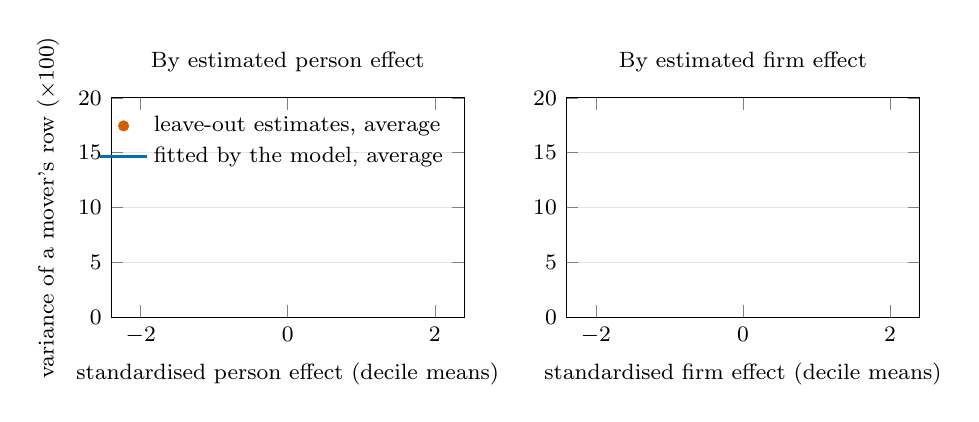
\begin{tikzpicture}
\begin{groupplot}[group style={group size=2 by 1, horizontal sep=1.3cm}, width=0.5\textwidth, height=0.36\textwidth,
  ymin=0, ymax=20, xmin=-2.4, xmax=2.4, ymajorgrids, grid style={gray!20},
  xlabel style={font=\footnotesize}, ylabel style={font=\footnotesize}, ticklabel style={font=\footnotesize},
  title style={font=\footnotesize}, legend style={font=\footnotesize, draw=none, fill=none, legend cell align=left}]
\nextgroupplot[title={By estimated person effect}, xlabel={standardised person effect (decile means)},
  ylabel={variance of a mover's row ($\times100$)}, legend style={at={(0.98,0.97)}, anchor=north east}]
\addlegendimage{only marks, mark=*, mark size=1.8pt, cmove}
\addlegendentry{leave-out estimates, average}
\addlegendimage{no marks, thick, cstay}
\addlegendentry{fitted by the model, average}
\addplot[cmove, only marks, mark=*, mark size=1.8pt, forget plot] coordinates {\figalphalo};
\addplot[cstay, thick, no marks, forget plot] coordinates {\figalphafit};
\nextgroupplot[title={By estimated firm effect}, xlabel={standardised firm effect (decile means)}]
\addplot[cmove, only marks, mark=*, mark size=1.8pt] coordinates {\figpsilo};
\addplot[cstay, thick, no marks] coordinates {\figpsifit};
\end{groupplot}
\end{tikzpicture}
\caption{Movers' rows by decile of the estimated effects: average leave-out estimate $\hat\sigma_i^2$ and average
fitted variance $\st_i^2$. Deciles are those of the stayers' estimated effects.}
\label{fig:profile}
\end{figure}

Figure~\ref{fig:profile} shows what the model works with and what it delivers. The averages of the leave-out
estimates vary a great deal. They are \R{dec.data.lo.bottom} times their average in the lowest decile of the
estimated person effect, \R{dec.data.lo.mid} times in the middle deciles and \R{dec.data.lo.top} times in the
highest, and they fall by more than half across the deciles of the firm effect. Stayers show the same pattern
at a lower level: the average $q_g$ (weighted by $T_g-1$) is \R{real.prof.alpha.stay.lo} times the stayers' overall average in the
lowest decile of the person effect, about \R{real.prof.alpha.stay.mid} times in the middle deciles and
\R{real.prof.alpha.stay.hi} times in the highest. The fitted variances follow the leave-out estimates closely
across the firm effect. Across the person effect they reproduce the U shape, but not exactly: they are
\R{dec.data.over.min} to \R{dec.data.over.max} above the leave-out averages in deciles 2 to 4 and
\R{dec.data.under.min} to \R{dec.data.under.max} below them in deciles 7 to 9. This fit, a quadratic in effects capped at three standard deviations, falls short there.

The scale of step~1 has a clear role in the data as well. The leave-out estimates average \R{real.lo.len1} for
one-year matches and \R{real.lo.longer.min} to \R{real.lo.longer.max} for longer ones. The variance of a mover's
yearly wages within a match is only \R{real.within_match_mean} on average: most of the error of a mover's row is
common to the years of the match, which is why nothing is assumed within a match and why the scale depends on
its length.

Can the decile averages of Figure~\ref{fig:profile} be trusted as a benchmark? Averaged over a fixed set of many
rows, the leave-out estimates estimate the average variance of those rows. Here the rows are sorted by an
estimated effect that depends on the same errors, which can distort the averages. Table~\ref{tab:deciles} adds
three simulated settings, where the truth is known. There the average leave-out estimate of a decile differs
from the average true variance by at most \R{dec.sim.gap.max}, upwards in the extreme deciles and about 5\%
downwards in the middle. The distortion in the data need not be the same.

\begin{table}[H]
\centering\small
\caption{Movers' rows by decile of the estimated person effect: average leave-out estimate $\hat\sigma_i^2$,
average fitted variance $\st_i^2$ and, in simulated data, average true variance ($\times100$)}\label{tab:deciles}
\begin{tabular}{@{}lcccccccccc@{}}
\toprule
 & \multicolumn{10}{c}{Decile of the estimated person effect (lowest to highest)} \\
\cmidrule(l){2-11}
 & 1 & 2 & 3 & 4 & 5 & 6 & 7 & 8 & 9 & 10 \\
\midrule
\tabinput{../note/gen/tab_deciles.tex}
\bottomrule
\multicolumn{11}{@{}p{0.92\textwidth}@{}}{\rule{0pt}{2.6ex}Deciles are those of the stayers' estimated person
effects, so movers' rows are spread unevenly over them (\R{dec.rows.min} to \R{dec.rows.max} of the rows per decile).
Simulated data: averages over \R{dec.reps} draws on the Veneto design (Section~\ref{sec:sim}); across the draws the
decile averages of the leave-out estimates vary by at most \R{dec.sd.max} (standard deviation). ``True variance''
is the average true variance of the rows that fall in the decile.}
\end{tabular}
\end{table}

In the simulated settings the fitted variances can also be compared with the truth. In the highest decile
they exceed the true variances in all three settings (by \R{dec.N1.fit.top}, \R{dec.N6.fit.top} and
\R{dec.N10.fit.top}), and in the setting without any profile in the lowest decile as well: the fit inherits
part of the distortion, which is the mechanism described in Section~\ref{sec:transfer}. What the discrepancies of the first panel mean for the
standard error, that is, how large $b(\Delta)/\V[\hat\theta]$ is on this panel, the table cannot say, and the
data cannot say it either, because movers' true variances are not observed. Scenario~10 of the simulation below
gives movers exactly the decile profile of the first panel; there the answer can be computed.

\subsection{Is any stayer or direction dominant?}

Sample versions of the two quantities in Proposition~\ref{prop:conc} are computed with the estimated
variances. For a stayer the first is
$\hat\phi_g=\sum_{i\in g}\st_i^2\,(4\hat m_i^{\,2}+2\hat r_i)/\hat\V[\hat\theta]$, where $\hat r_i$ is the simulated
value of $\sum_\ell C_{i\ell}^2\st_\ell^2$ from 32 draws as in \eqref{eq:sim}; the same ratio is formed for each
mover's row. The second is $\hat\lambda_{\max}^2/\hat\V[\hat\theta]$, with $\hat\lambda_{\max}^2$ from 20 power
iterations on the matrix with entries $\st_iC_{i\ell}\st_\ell$. These are concentration ratios, not exact shares:
$\hat m_i^{\,2}$ overstates $m_i^2$, so the $\hat\phi_g$ do not add up to one. All are small. The largest
$\hat\phi_g$ is \R{real.max_stayer_share}, the largest ratio of a mover's row \R{real.max_mover_share}, and
$\hat\lambda_{\max}^2/\hat\V[\hat\theta]$ is between \R{real.lambda.min} and \R{real.lambda.max} for the four
components.

\subsection{Simulation}\label{sec:sim}

\paragraph{Design.} The effects fitted on the panel serve as the truth, and new errors are drawn for every
person-year, \R{sim.reps} times in each of ten scenarios (\R{sim.failures} draws failed). Each draw runs the
estimator exactly as on the data: effects, leverages of movers from the same 1{,}600 projections, the two steps
of the model for movers with estimated effects in the profile, and 16 draws for the double sum. The variance
of $\hat\theta$ is computed from \eqref{eq:V} for each scenario. Appendix~\ref{app:sim} defines the scenarios and
reports how each was realised. In scenarios 1 to 7 movers and stayers share one variance profile. Scenario~1
has none. In scenarios 2 to 5 the profile is quadratic in the standardised person effect, as the model's is,
with one difference: the model caps the standardised effects at three standard deviations and the scenarios do
not. Scenario~6 uses a step profile taken from the data, the stayers' average sample variance by decile of the
person effect, and scenario~7 a profile that is log-linear in the wage level. Scenarios 3 to 5 also violate A3
(fat tails, skewness). In scenarios 8 to 10 movers have a profile of their own. In 8 and 9 their variances rise
three times as fast with the distance from the mean wage as the stayers', or not at all. In both, the movers'
profile lies in the model's quadratic basis before capping; exact recovery by the two regressions requires in
addition the condition on the scale in Corollary~\ref{cor:transfer}. Scenario~10 is calibrated to the data and is
not within the model: movers follow the decile profile of their own leave-out estimates in the first row of
Table~\ref{tab:deciles}.

\begin{table}[H]
\centering\small
\caption{Simulation on the Veneto design: square root of the mean variance estimate over the true variance}\label{tab:sim}
\begin{tabular}{@{}rlcccccccccc@{}}
\toprule
 & & \multicolumn{4}{c}{With the model for movers} & & \multicolumn{4}{c}{With movers' true variances} \\
\cmidrule(lr){3-6}\cmidrule(l){8-11}
 & Scenario & $\sigma^2_\alpha$ & $\sigma^2_\psi$ & $\sigma_{\alpha,\psi}$ & $\sigma^2_{\alpha+\psi}$ & & $\sigma^2_\alpha$ & $\sigma^2_\psi$ & $\sigma_{\alpha,\psi}$ & $\sigma^2_{\alpha+\psi}$ \\
\midrule
\tabinput{../note/gen/tab_sim.tex}
\bottomrule
\multicolumn{11}{@{}p{0.9\textwidth}@{}}{\rule{0pt}{2.6ex}A value of 1 means that the mean variance estimate
equals the true variance; the entry is the root-mean-square standard error over the true one.
\R{sim.reps} draws per scenario. In scenarios 8 to 10 movers have a profile of their own. Right panel:
\eqref{eq:Vhat} with $\st_i^2=\sigma_i^2$ on movers' rows, which isolates the stayers' part.}
\end{tabular}
\end{table}

\begin{table}[H]
\centering\small\setlength{\tabcolsep}{4.6pt}
\caption{Simulation on the Veneto design: coverage of the 95\% interval}\label{tab:simcov}
\begin{tabular}{@{}rlcccccccccc@{}}
\toprule
 & & \multicolumn{4}{c}{With the model for movers} & & \multicolumn{4}{c}{With movers' true variances} \\
\cmidrule(lr){3-6}\cmidrule(l){8-11}
 & Scenario & $\sigma^2_\alpha$ & $\sigma^2_\psi$ & $\sigma_{\alpha,\psi}$ & $\sigma^2_{\alpha+\psi}$ & & $\sigma^2_\alpha$ & $\sigma^2_\psi$ & $\sigma_{\alpha,\psi}$ & $\sigma^2_{\alpha+\psi}$ \\
\midrule
\tabinput{../note/gen/tab_simcov.tex}
\bottomrule
\multicolumn{11}{@{}p{0.9\textwidth}@{}}{\rule{0pt}{2.6ex}Share of draws in which
$\hat\theta\pm1.96\,\hat\V[\hat\theta]^{1/2}$ covers the true $\theta$. With \R{sim.reps} draws the Monte Carlo
standard error is about 0.015.}
\end{tabular}
\end{table}

\begin{table}[H]
\centering\small
\caption{The model's error at fixed characteristics, $[1+b(\Delta)/\V[\hat\theta]]^{1/2}$, against the simulated ratio}\label{tab:bdelta}
\begin{tabular}{@{}rlcccccccccc@{}}
\toprule
 & & \multicolumn{4}{c}{At fixed characteristics} & & \multicolumn{4}{c}{As implemented (Table~\ref{tab:sim})} \\
\cmidrule(lr){3-6}\cmidrule(l){8-11}
 & Scenario & $\sigma^2_\alpha$ & $\sigma^2_\psi$ & $\sigma_{\alpha,\psi}$ & $\sigma^2_{\alpha+\psi}$ & & $\sigma^2_\alpha$ & $\sigma^2_\psi$ & $\sigma_{\alpha,\psi}$ & $\sigma^2_{\alpha+\psi}$ \\
\midrule
\tabinput{../note/gen/tab_bdelta.tex}
\bottomrule
\multicolumn{11}{@{}p{0.9\textwidth}@{}}{\rule{0pt}{2.6ex}Left: the two steps of the model are run with the true
variances as outcomes and the true effects as characteristics; this gives $v_i^*$, $\Delta_i=v_i^*-\sigma_i^2$ and
$b(\Delta)$ from \eqref{eq:b}, with no simulated outcomes. It concerns the model for movers only; the stayers' departures from A3 in scenarios 3 to 5 are not in it.
Right: the left panel of Table~\ref{tab:sim}. The panels differ in everything else: estimated effects, the
sampling error of the two fits, the stayers' part, projected weights, and the projection of the covariance
matrix described in the text.}
\end{tabular}
\end{table}

\paragraph{Findings.} \emph{The stayers' part.} With movers' true variances (right panels of
Tables~\ref{tab:sim} and~\ref{tab:simcov}) the ratio is between \R{sim.or.noskew.min} and \R{sim.or.noskew.max}
in the eight scenarios without skewness, including scenario~3 with fat tails. In the two scenarios with skewed
stayers' errors it is \R{sim.N4.or.sum} and \R{sim.N5.or.sum} for the variance of the sum: the shift that
Section~\ref{sec:results} predicts, with the predicted signs. The simulations thus agree with
Proposition~\ref{prop:mean} and the formulas for departures from A3, although those are for exact weights and
these runs use projected ones.

\emph{With the model for movers.} Across the \R{sim.n.cells} cells the ratio of Table~\ref{tab:sim}, the
root-mean-square standard error over the true one, is between \R{sim.all.min} and \R{sim.all.max}. It is below
0.95 in \R{sim.n.below95} cells and above 1.05 in \R{sim.n.above105} (counts here and below are before
rounding). For $\sigma^2_\alpha$ the ratio is between
\R{sim.comp.alpha.min} and \R{sim.comp.alpha.max}, for $\sigma^2_\psi$ between \R{sim.comp.psi.min} and
\R{sim.comp.psi.max}, for the covariance between \R{sim.comp.cov.min} and \R{sim.comp.cov.max}, and for the
variance of the sum between \R{sim.comp.sum.min} and \R{sim.comp.sum.max}. The ratio is thus below one
by \R{sim.under.max} at most (the variance of the sum in scenario~4, where the benchmark with movers' true
variances in the right panel is itself about three percent low), and above one by up to \R{sim.over.max}. The largest ratios are those for
$\sigma^2_\psi$ in the four scenarios with worker-specific variance factors, and for the sum in two of them. In
scenario~10, where movers have the decile profile of the data, the ratios are \R{sim.N10.alpha}, \R{sim.N10.psi},
\R{sim.N10.cov} and \R{sim.N10.sum}. The coverage of the 95\% interval is between \R{sim.all.cov.min} and
\R{sim.all.cov.max} (Table~\ref{tab:simcov}), against \R{sim.or.cov.min} to \R{sim.or.cov.max} with movers' true
variances. No draw failed. In no draw did the last floor bind for more than \R{sim.floor.final.max} of movers'
rows, and the floor on the scale never bound. The Monte Carlo standard error of the ratios is at most \R{sim.ratio.mcse.max}. One step of the prototype in
these runs is not in Section~\ref{sec:estimator}: before the variances were read off, negative eigenvalues of the
estimated covariance matrix of the three base components were set to zero. This can only raise a variance
estimate, and it applies to Tables~\ref{tab:sim} to~\ref{tab:bdelta} (right panel). On
the data that matrix is positive definite, with a smallest eigenvalue of \R{real8.eig.ratio} of the largest, so
the projection changes nothing there. For these simulated draws it was not recorded whether it changed
anything. The validation runs of Section~\ref{sec:validation} use the estimator without the projection, and on
the same design they give the same ratios to within \R{val.six.devdiff.max}.

\emph{The model at fixed characteristics.} Table~\ref{tab:bdelta} separates the model for movers from the
rest. Its left panel evaluates the quantity of A4 on this design: the error $b(\Delta)$ of the model when its
two steps see the true variances and the true effects. In scenarios 1 and 9 the model's error is zero to three decimals. In the other
eight, $[1+b(\Delta)/\V[\hat\theta]]^{1/2}$ is between \R{sim.bd.other.min} and \R{sim.bd.other.max} for the first
three components and between \R{sim.bd.sum.min} and \R{sim.bd.sum.max} for the variance of the sum: at fixed
characteristics the model would understate that standard error by \R{sim.bd.sum.short.min} to
\R{sim.bd.sum.short.max}. Two sources can be told apart. One is the cap on the standardised effects. In
scenarios 2 to 5 and 8 the true variances keep growing with the square of the effect beyond three standard
deviations, where the model holds its profile constant. Few rows lie there, \R{sim.cap.N4.rows3} of movers'
rows, but in scenario~4 they carry \R{sim.cap.N4.first3.whole} of the first term of \eqref{eq:V} for the variance
of the sum (\R{sim.cap.N4.first3} of the movers' part). In that scenario the entry of Table~\ref{tab:bdelta} for the sum is \R{sim.cap.N4.3.sum} with the cap at
3; with a cap at 4 it would be \R{sim.cap.N4.4.sum}, at 6 \R{sim.cap.N4.6.sum}, and without a cap
\R{sim.cap.N4.none.sum}. In scenario~8 the same four numbers are \R{sim.cap.N8.3.sum}, \R{sim.cap.N8.4.sum},
\R{sim.cap.N8.6.sum} and \R{sim.cap.N8.none.sum}. The cap protects the fit from a few rows with extreme estimated effects, and this is its
price when variances keep rising in the tails. The other source is easy to overlook. In scenarios 2, 3, 6 and
10 every worker has a variance factor of its own, which the matches of a mover share and which no
characteristic in the model captures. Such errors average out in the first part of $b(\Delta)$, in expectation
over the factors, but not in its second, the double sum, which is negative when the errors of the model are
positively related within a worker. For $\sigma^2_{\alpha+\psi}$ the double sum lowers the mean of the variance
estimate by \R{sim.bdquad.mix.min} to \R{sim.bdquad.mix.max} of the variance in these four scenarios, and by at
most \R{sim.bdquad.other.max} elsewhere (Table~\ref{tab:regime}); it contains all errors of the model, not only
those from the worker factors. A model that is right about the average variance of every group of rows can
therefore still give a standard error that is too small.

\emph{As implemented.} The procedure as implemented (right panel of Table~\ref{tab:bdelta}) lies above its
fixed-characteristics counterpart in \R{sim.bd.above.all} of the \R{sim.n.cells} cells; for the variance of the
sum the difference is between $\R{sim.bd.diff.sum.min}$ and $\R{sim.bd.diff.sum.max}$ (before rounding). The
ratios of Table~\ref{tab:sim} are therefore the net of two opposing contributions: a model error that lowers the
variance estimate, and an often larger net contribution of the implementation in the other direction. The two
panels differ in several ways at once (estimated effects in place of true ones, noisy outcomes in the two fits,
the stayers' part in scenarios 3 to 5, the projection of the covariance matrix), so the comparison does not
isolate a cause. In scenario~1 the model is exact at fixed characteristics, and as implemented the ratio for
the variance of the sum is \R{sim.N1.sum}: an upward discrepancy of the implementation with no model error
behind it. We have no result that predicts its sign in other designs; Section~\ref{sec:validation} looks at
two.

\emph{What the simulations do not show.} They use one design and ten scenarios of our choosing, and the form of
the model was chosen on the same scenarios (Appendix~\ref{app:sim}). They show how the standard error behaves when
movers' variances are as specified. They cannot show how large $b(\Delta)/\V[\hat\theta]$ is on the Veneto panel
itself, where movers' variances are not observed; scenario~10 is the closest we can come.

\subsection{Validation: fresh draws and two further designs}\label{sec:validation}

The simulations above served to choose the model. After that choice the estimator was frozen and run once
more, with acceptance thresholds written down before any task ran. There are three runs.
\begin{itemize}
\item \emph{Six-year panel, fresh draws.} The ten scenarios of Table~\ref{tab:sim} with new error draws.
\item \emph{A three-year window.} The years 1999 to 2001 of the same data: \R{val.y3.n.person_years} person-years
of \R{val.y3.n.workers} workers at \R{val.y3.n.firms} firms, \R{val.y3.n.rows} rows. Stayers have two or three
years (\R{val.y3.share.stayer2} of them two), and their rows carry most of the first term for the variance of
the sum.
\item \emph{Half of the workers.} A random half of the workers of the six-year panel:
\R{val.half.n.person_years} person-years of \R{val.half.n.workers} workers at \R{val.half.n.firms} firms,
\R{val.half.n.rows} rows, with a thinner network of moves.
\end{itemize}
Each sub-panel was pruned to the set in which every mover's match can be left out, the effects fitted on it
serve as its truth, and six of the ten scenarios (1, 2, 4, 6, 8 and 10) were run on it. Every cell has 200
draws. In these runs the estimator is that of Section~\ref{sec:estimator}, with no projection of the covariance
matrix (the cases in which that section gives no standard error did not arise). A draw whose variance estimate is not positive is counted and enters the coverage as a
miss; a draw that fails altogether fails the run.

The thresholds were, for every scenario and component, a ratio as in Table~\ref{tab:sim} between
\R{val.acc.ratio_min} and \R{val.acc.ratio_max} and a coverage of the 95\% interval of at least
\R{val.acc.coverage_min}; and for every run, an average coverage of at least \R{val.acc.mean_coverage_min}, no
failed draw, no variance estimate that is not positive, and floors that bind for at most \R{val.acc.max_floored}
of movers' rows in any draw. These are tolerances chosen in advance. Meeting them does not establish a
coverage of 95\%: with 200 draws the coverage of a cell is known to about $\pm0.03$.

\begin{table}[H]
\centering\footnotesize\setlength{\tabcolsep}{4.5pt}
\caption{Validation runs: root-mean-square standard error over the true one, and coverage, by run}\label{tab:val}
\begin{tabular}{@{}lccccccc@{}}
\toprule
 & & \multicolumn{4}{c}{Ratio, smallest to largest over scenarios} & & Thresholds \\
\cmidrule(lr){3-6}
Run & Scenarios & $\sigma^2_\alpha$ & $\sigma^2_\psi$ & $\sigma_{\alpha,\psi}$ & $\sigma^2_{\alpha+\psi}$ & Coverage & met \\
\midrule
\tabinput{../note/gen/tab_val.tex}
\bottomrule
\multicolumn{8}{@{}p{0.9\textwidth}@{}}{\rule{0pt}{2.6ex}200 draws per scenario; coverage is the smallest and
the largest over scenarios and components. Appendix~\ref{app:sim} gives every cell.}
\end{tabular}
\end{table}

Two of the three runs met every threshold; the three-year window did not (Table~\ref{tab:val}). On the
six-year panel the fresh draws reproduce Table~\ref{tab:sim}: the forty ratios lie between
\R{val.six.ratio.min} and \R{val.six.ratio.max} and differ from those of the earlier runs by at most
\R{val.six.devdiff.max}, although this run has no projection of the covariance matrix. That step was therefore
immaterial; in all \R{val.all.draws} validation draws the matrix was positive definite, with a smallest
eigenvalue of at least \R{val.all.eig.min} of the largest. Coverage on the six-year panel is between
\R{val.six.cover.min} and \R{val.six.cover.max}. With half of the workers the ratios are between
\R{val.half.ratio.min} and \R{val.half.ratio.max} and coverage is between \R{val.half.cover.min} and
\R{val.half.cover.max}. In the three-year window the ratios are between \R{val.y3.ratio.min} and
\R{val.y3.ratio.max}, and the upper threshold of \R{val.acc.ratio_max} is exceeded in two cells, both for
$\sigma^2_\psi$: \R{val.y3.N6.psi.d3} in scenario~6 and \R{val.y3.N10.psi.d3} in scenario~10. Coverage there is between
\R{val.y3.cover.min} and \R{val.y3.cover.max}. In no run did a draw fail or a variance estimate come out zero or
negative, and floors bound for at most \R{val.all.floor.max} of movers' rows in any draw.

The validation adds two things. First, the results of Section~\ref{sec:sim} are not an artefact of the draws on
which the model was chosen, or of the projection. Second, the upward discrepancy is not the same in every
design. For $\sigma^2_\psi$ the largest ratio rises from \R{val.six.psi.max} on the six-year panel to
\R{val.half.psi.max} with half of the workers and \R{val.y3.psi.max} in the three-year window, the two designs
with fewer observations behind each estimated effect. On a short panel the standard error of
$\hat\sigma^2_\psi$ can thus be too large by a sixth. Across the \R{val.all.cells} cells of the three runs the ratio
is below 0.95 in \R{val.all.n.below95} and above 1.10 in \R{val.all.n.above110}. As before, none of this says how
large the model's error is on the real panel.

\section{Implementation in \fevc{} 0.6.0}\label{sec:impl}

The prototype behind Sections~\ref{sec:q1} and~\ref{sec:evidence} preceded the package. \fevc{} implemented the
method between November 13 and 14, 2026, and released it in 0.6.0 as its only standard-error method and its
default, \code{inference(auto)}; \code{inference(none)} gives point estimates only. What the command does is
specified in the package's \code{fevc/docs/INFERENCE.md}; where this note and that guide differ, the guide
describes the command. This section lists the differences, states the rule by which the default chooses an
interval, and summarises the package's own Monte Carlo evidence.

\subsection{Differences from the prototype}\label{sec:impl-diff}

\begin{enumerate}[leftmargin=1.6em,itemsep=3pt]
\item \textbf{Deletion modes and repeat-measurement sets.} The propositions and the prototype cover match
deletion, where stayers are the only sets of rows with identical regressors (Section~\ref{sec:scope}); the control
term of Section~\ref{sec:controls} is derived for both modes. 0.6.0 also covers observation deletion,
where every worker--firm cell with two or more observations, a mover's match included, is a set, with the pair
weight $B_{ii}/(1-P_{ii})$ for every target; and mover-only populations. The only sets are deletion units that
share a worker--firm cell. Co-mover groups and cycles of matches, which earlier drafts considered, are not used.
\item \textbf{Fitting the model for the other units.} The two steps and the floors are those of
Section~\ref{sec:transfer}. In addition, each step keeps at most one coefficient per hundred fitted units,
shortening the basis in a fixed order; a term that the others span is dropped, also in a fixed order, where
Section~\ref{sec:transfer} withholds the standard error; with fewer than a hundred units outside sets the model is fitted on all units
of movers; the final floor also applies to the sample variance of a set; and the pass stops with
\code{JLA\_CONSTRAINT\_FAILED} when the mean leave-out estimate is not positive (as in Section~\ref{sec:transfer}) or when every
fitted variance is floored.
\item \textbf{Leverages, projections and draws.} The prototype uses the exact $P_{ii}=1/T_g$ and
$B_{ii}=A_{gg}/T_g^2$ for stayers and 1{,}600 projections for movers, without a finite-projection correction
(Section~\ref{sec:computation}). 0.6.0 takes them from the route: on the native route the pass uses the JLA
leverages of the point estimate (200 projections by default) and checks them against its bias correction; the
Mata \code{algorithm(jla)} stage draws its own projections; exact leverages exist only on the Mata
\code{algorithm(exact)} route. The stayers' exact values are not substituted. The
default is eight pseudo-noise draws (\code{inferencedraws()}), not 16, and the linear systems are solved
iteratively, not by a factorisation.
\item \textbf{Kurtosis.} The pair term is the one for errors with the kurtosis of the normal distribution; the
variant for another stated kurtosis (Appendix~\ref{app:proofs}) is not offered.
\item \textbf{No projection of the covariance.} The prototype's simulation of Section~\ref{sec:sim} set negative
eigenvalues of the estimated covariance of the three base components to zero. 0.6.0 reports the covariance as
computed; a variance estimate that is not positive withholds the normal interval of that component, and the
default then reports its $q=1$ interval where it exists.
\item \textbf{Controls.} The prototype treats the control coefficients as known. 0.6.0 includes their estimation
to first order, as derived in Section~\ref{sec:controls}: the variance of the fixed-offset estimate under the noise
of the control-adjusted outcome, on every route. Not covered: the joint estimate's additional term in the control
index (Section~\ref{ctl:joint}), error variances that move with a control inside a cell (item~7 of
Section~\ref{ctl:est}), the within-unit covariance that the pseudo-noise omits (item~1), and poorly identified
coefficients. The repair $\hat Q_{\rm full}$ of item~1 is not implemented.
\item \textbf{Centring.} The propositions and the prototype treat the sample mean used for centring as a constant. Under
\code{centering(mean)} the package centres the pseudo-noise as the outcome, so no fixed-mean approximation is made;
under \code{centering(corrected)} the standard error is that of the mean-centred estimate, with the increment
held fixed (Section~\ref{sec:centring}).
\item \textbf{Leading direction.} The prototype uses power iteration (stopped at 200 steps; one Veneto case did
not converge). 0.6.0 uses a thick-restart Lanczos iteration in the $S_{xx}$ inner product (basis six, three Ritz
vectors kept, stopped at a relative residual of $10^{-3}$ or after 40 solves, each search started from the
previous target's direction), and a dense eigendecomposition on the exact Mata route
(Appendix~\ref{kss:app:lanczos}). The draws of the pass are reused for the remainder: about 90 solves in all with
the default eight draws, where the pass alone takes 35.
\item \textbf{One interval per component.} Section~\ref{sec:q1} gives the $q=1$ interval for designs with one weak direction
and a screening value without a validated threshold, and leaves the choice between the two intervals open.
0.6.0 chooses per component by the rule of Section~\ref{sec:impl-rule}.
\item \textbf{The other variance models.} Appendix~\ref{app:cost} compares the cost with the KSS Matlab package,
with \fevc's structured route under \code{inference(highrank)}, and with the leave-out residual standard error that
was the development default at the time (never released). 0.6.0 removed those models (\code{target\_lowess},
\code{structured\_common}, \code{structured\_leverage}, \code{leaveout\_residual}); \code{inference(highrank)} now
selects the normal intervals of this method.
\end{enumerate}

The prototype's failed tolerances stand: in the validation of Section~\ref{sec:validation} the standard error of the
firm variance in the three-year window was up to 16\% too large, beyond the registered 15\%, and the $q=1$
confirmation of Section~\ref{sec:q1sim} missed its length tolerance in one design without a bottleneck.

\subsection{The interval of every component}\label{sec:impl-rule}

Under \code{inference(auto)} a component receives the $q=1$ interval of Section~\ref{sec:q1} when its leading
direction carries more than ten per cent of the estimated sampling variance,
\[
\frac{4\lambda_1^2\max(\hat b_1^{\,2}-V_b,0)\,V_b+2\lambda_1^2V_b^2}{\hat\V[\hat\theta]},
\]
with $V_b$ the estimated variance of $\hat b_1$, or when the high-rank variance estimate \eqref{eq:Vhat} is not
positive; otherwise it receives the normal interval. The variance of the sum, whose non-zero eigenvalues are all
equal (Section~\ref{sec:q1}), keeps the normal interval. A component with the $q=1$ interval has no standard error,
and \code{e(V)} is posted only when every component has a normal interval; it is then the four-by-four covariance
of the components, mapped from the three base components. \code{inference(highrank)} asks for normal intervals
only and \code{inference(q1)} for the $q=1$ interval wherever it exists; both are strict, while the default
returns point estimates with a reason when the standard errors cannot be computed. The share is a ratio of two
estimates and can exceed one. The critical value of the $q=1$ interval is simulated with 100{,}000 draws.

The statistic and the threshold were chosen afterwards, on simulations through the command (\code{dev1} below),
confirmed on new designs (\code{conf2}), and the threshold was fixed by the owner on November 14, 2026. Over the
96 cases of \code{dev1}, the rule's lowest coverage is 0.937, against 0.940 with a threshold of 5\% and 0.935 with
20\%; it reports the $q=1$ interval for 4.3\% of the components without a bottleneck and posts \code{e(V)} in 89\%
of those samples, against 9.8\% and 76\% at 5\%. On three panels of the Veneto data (2.3 to 5.2 million
person-years, both deletion modes) every component receives the normal interval under this rule (shares 0.03\% to
8.1\%), and the default costs 24\% to 30\% more time than the point estimates alone (16 threads). Neither KSS nor
this note has a theoretical result for this data-dependent choice, and two or more dominant directions are not
covered.

\subsection{The package Monte Carlo evidence}\label{sec:impl-mc}

The package's own Monte Carlo passes the plain Stata command, with a plugin built from a named commit, through
two-block synthetic panels of about 48{,}000 person-years, from no bottleneck to a strong one, with error variances
that follow or violate the fitted model and normal or skewed errors, under match and observation deletion. Each
run's manifest was frozen before any task ran. The harness is \code{fevc/tools/default\_interval/} and the records
are in \code{fevc/docs/default\_interval/}. Table~\ref{tab:impl-mc} summarises the runs that decide the rule and
its confirmation.

\begin{table}[H]
\centering\small\setlength{\tabcolsep}{4pt}
\caption{Package Monte Carlo runs of the default interval}\label{tab:impl-mc}
\begin{tabular}{@{}lllccccc@{}}
\toprule
 & & & Designs & & & \multicolumn{2}{c}{Coverage} \\
\cmidrule(l){7-8}
Run & Kind & Commit & $\times$ 2 modes & Fits & Verdict & lowest & mean \\
\midrule
\code{dev1} & development & \code{250a760c} & 16 & 32{,}000 & none & 0.937$^a$ & -- \\
\code{conf1} & confirmation & \code{fb49e16d} & 20 & 40{,}000 & FAIL & 0.937$^b$ & 0.960$^b$ \\
\code{conf2} & confirmation & \code{fb49e16d} & 20 & 40{,}000 & PASS & 0.930 & 0.9593 \\
\code{dev3\_controls} & development & \code{02d7955f} & 13 & 13{,}000 & none & 0.918 & 0.962 \\
\code{conf3\_controls} & confirmation & \code{f3938986} & 20 & 40{,}000 & PASS & 0.923 & 0.9602 \\
\bottomrule
\multicolumn{8}{@{}p{0.92\textwidth}@{}}{\rule{0pt}{2.6ex}Coverage is that of the reported interval over the
cases (design, deletion mode and component); a
replication without an interval counts as not covered. $^a$~The 10\% rule evaluated on the draws of \code{dev1},
which ran with the first threshold of 5\%. $^b$~The verdict failed on the inventory: one fit returned point
estimates (the documented fallback after \code{JLA\_CONSTRAINT\_FAILED}), the harness of the time rejected its
task, and the verdict stands as registered. The numbers are for information only and count that fit as a
replication without an interval. \code{dev1},
\code{conf1} and \code{conf2} have no controls; \code{dev3\_controls} and \code{conf3\_controls} have controls in
every design.}
\end{tabular}
\end{table}

\code{conf2} met all of its tolerances: none of its 40{,}000 fits failed or fell back to point estimates, at most 6
of the 1{,}000 replications of a case had no interval, the lowest coverage is that of the variance of the sum under
match deletion in a design with 1{,}000 bridging workers, and without a bottleneck the reported interval is at most
1.059 times as long as the normal one and \code{e(V)} is posted in 89\% of the samples. The same replications
judged with the normal interval alone have a lowest coverage of 0.789. \code{conf3\_controls} ran the same twenty
design shapes, replications and tolerances with new seeds and controls in every design, in a fixed rotation of
four kinds; its lowest cases are the worker and firm variances (0.923 and 0.926) in a design whose blocks differ,
with the control loaded on the worker effect, where their standard errors are 8\% and 7\% short. A compatibility
review carries its claim from \code{f3938986} to the original 0.6.0 candidate build commit \code{d4b2d942}: 36
default requests give byte-identical results. The released 0.6.0 plugins were built later, from \code{2082f209};
the review does not extend the simulation claims to the subsequent Stata~15 compatibility changes or to the
revised exact eigensolver, so these confirmations are of pre-release builds, not of the released binaries. Before the control term, \code{dev2\_controls} found the standard error of the variance of
the sum 9\% to 16\% too small with one adverse control; on the same outcome draws with the term of
Section~\ref{sec:controls}, \code{dev3\_controls} gives 0.97 to 1.04 of the spread and coverage of 0.938 to 0.956.
Its lowest case (the covariance, with a control index as large as the effects and no bottleneck, under match
deletion) has a standard error 12\% too small; under \code{nuisance(fixedoffset)} the same design gives, under
match deletion, 0.99 to 1.07 of the spread and coverage of 0.948 to 0.962 (\code{dev4\_fixedoffset}), so the
shortfall belongs to the joint estimate's additional term of Section~\ref{ctl:joint}, not to the standard error of
the fixed-offset estimate. (\code{deletion(observation)} with \code{nuisance(fixedoffset)} is not covered by the
standard errors: the command returns point estimates only, as all 1{,}000 such fits of \code{dev4\_fixedoffset}
did.) The same term shows where the two blocks of firms differ by three log points and the control loads on the
firm effect: under the default the standard error of the worker variance, and in two of three designs that of the
firm variance, is 0.87 to 0.94 of the spread (\code{dev6\_shapes}, \code{dev7\_adv}), and under the fixed offset,
with match deletion, 0.92 to 0.99 (\code{dev7\_fixedoffset}). Not covered by
\code{conf3\_controls}, by design: a control index as large as the effects, error variances that move with a
control inside a cell, and a control loaded on the firm effect where the blocks differ. This is simulation
evidence for designs with one bottleneck at most and independent errors; it is not a coverage guarantee, and it
does not cover two or more dominant directions.

%=====================================================================================
\section{Comparison with the KSS standard errors}\label{sec:kss}

This section compares three ways of computing standard errors for leave-out (KSS) variance components: the
split-sample estimator of Kline, Saggio and S{\o}lvsten (2020, Section~5.2; ``KSS'') as implemented in their
Econometrica replication code; the model-based estimator of the KSS Matlab package, which replaces each error
variance by a smooth fit; and the repeat-measurement estimator that \fevc{} 0.6.0 reports by default. The first
part explains how each works, where its computing time goes, and what it assumes. The second part runs \fevc{} on
the samples for which KSS published standard errors and confidence intervals (Table~IV), next to KSS's own code
run on the same samples, and on outcomes drawn with a known truth.

\subsection{Summary of the comparison}\label{kss:sec:summary}
\paragraph{What was done.} The six samples of KSS Table~IV were rebuilt from the raw data with KSS's own,
unchanged code; they match KSS Table~I to within 0.01\%. On identical rows, KSS's paper method (their
Table~IV code), the model-based estimator of the KSS Matlab package (GitHub and replication versions) and
\fevc{} 0.6.0 were run. Then, on the two older-worker networks, where the methods disagree most, outcomes were
drawn with a known truth from KSS's own Monte Carlo design, and every method was run on the same draws (1{,}000
for \fevc, 100--200 for the KSS codes, which take 15 minutes to over an hour per draw).

\paragraph{Point estimates.} With two periods and observation deletion, \fevc{} and KSS compute the same
estimator. \fevc{} reproduces KSS's estimates to within its numerical error once the year effect is handled as
KSS handle it (\code{nuisance(fixedoffset)}) and enough random projections are used. Its default lies between
0.9\% below and 0.8\% above KSS: re-estimating the year effect in every leave-out fit raises it by 0.2--0.9\%,
and its 200 default projections add numerical noise of 10--12\% of the standard error on the older-worker
samples.

\paragraph{Standard errors on the real data (firm variance).}
\begin{itemize}
\item On the three leave-one-out samples, KSS's standard error is the largest, by design: 15--22\% of movers have
no split-sample estimator and get a conservative variance. \fevc{} and the model-based estimator agree with each
other (0.00049 and 0.00048 pooled, 0.00052 and 0.00049 younger, 0.00199 and 0.00196 older).
\item On the pooled and younger leave-two-out samples all methods agree. On the older-worker leave-two-out
sample, where one direction dominates, they range from 0.00094 (\fevc{} default) to 0.00137 (KSS; 0.00141 on a
second call of the same code), yet the
reported $q=1$ intervals are almost the same: $[.0155,.0220]$ for KSS and $[.0154,.0218]$ for \fevc.
\item \fevc{} reports the $q=1$ interval on exactly the three samples where KSS's $q=1$ and normal intervals
differ.
\end{itemize}

\paragraph{Against a known truth (firm variance, older workers).}
\begin{itemize}
\item \emph{Leave-two-out.} KSS's standard error is 10\% too large; \fevc's is 6\% too small by default and on
target without centering; the model-based one is 5\% too small, and its $q=1$ interval is invalid on 19\% of the
draws: it excludes its own estimate, and on a third of those draws the variance estimate is also negative. The reported intervals cover
97.5\% (KSS, $q=1$) and 98.9\% (\fevc, which chose $q=1$ on every draw) at the same median length; the
model-based $q=1$ interval covers 76.5\%.
\item \emph{Leave-one-out.} KSS's standard error is 44\% too large (KSS's own Table~V: 28\%) and its intervals
cover every draw at 30\% more length than \fevc's. The model-based estimator and \fevc{} are within 2--4\%;
\fevc's reported interval covers 97.2\%.
\end{itemize}

\paragraph{Worker variance and covariance.} KSS's paper method does not estimate them. On the real data \fevc{}
and the model-based estimator agree within 6--11\% on the pooled and older samples, and \fevc's are 12--25\% larger
on the younger samples. In the simulation \fevc{} is within 7\% on the leave-one-out sample but 10--17\% too small
on the older leave-two-out sample, where the model-based estimator is on target; this does not change when the
noise is split between the two years. \fevc's reported ($q=1$) intervals still cover 96--98\% there. A diagnostic
traces the shortfall to about thirty movers on the network's bottleneck, on whom the leading direction of these
two components rests: in the simulated design their noise depends on their weight in the firm-variance estimator,
which \fevc's variance model does not see, and the model gives them under half their true variance. High leverage as
such is not the cause. The design favours the model-based estimator, whose smoother uses exactly that weight, and
the dependence itself comes from a noisy own-sample fit whose sign is opposite to KSS's pooled fit.

\paragraph{Computing time.} \fevc{} takes 18--96 seconds per sample for all four components and their covariance.
KSS's paper method takes 13 minutes (older leave-two-out) to 10 hours (younger leave-two-out) for its two calls on
the firm variance alone, 15 hours for the first call alone on the younger leave-one-out sample, and had not finished
the first call on either pooled sample when it was stopped after 23 hours; the model-based code takes 10 minutes to
10 hours.

\paragraph{Problems in the KSS code.} The critical values for $q=2$ are not shipped, so the $q=2$ intervals of
Table~IV cannot be reproduced; their randomness is unseeded, so two runs differ by 0.5--8\% in the standard error;
the variance routine of the paper method subtracts a constant where the projection on the leading direction
appears to be meant, which affects the $q=1$ interval by an amount not measured here; the replication package's
model-based routine fails when eigenvalue diagnostics are requested; and the model-based estimator returns
negative variance estimates, which their code turns into imaginary standard errors.

\paragraph{Caveats.} The simulation fits KSS's design on each sample rather than on the pooled sample, as KSS do.
In KSS's design stayers' wages carry no noise, and under observation deletion a two-period mover has no repeat
measurement, so the simulation tests \fevc's fitted variance model for movers, not its repeat-measurement part. The
paper method's reruns on the two pooled samples were stopped after 23 hours, before their first call had finished;
for those samples the tables show KSS's published values only.

\paragraph{For \fevc.} Three points follow. (i) For samples like these the default 200 projections leave
noticeable numerical noise in the point estimate; a larger or adaptive default would remove it, at about two to
three times the run time for 2{,}000 projections.
(ii) Under observation deletion with two periods the centering changes the standard error, not the estimate; the
default was 6\% low on the leave-two-out simulation and on target on the leave-one-out one. (iii) When one
direction dominates a component, its standard error depends on the variances of the few movers that direction
rests on, and \fevc's variance model, which uses the rank of leverage and the estimated effects, cannot follow a
variance that depends on the mover's weight in the target, as KSS's design does. Adding the target diagonals to the
features of the scale would nest the inputs of KSS's smoother; whether it is worth it depends on whether real error
variances behave that way, which a design without this dependence, or real repeat measurements, would have to show.


%=====================================================================================
\subsection{The two KSS estimators}\label{kss:sec:methods}

\paragraph{What all three estimate.} Every method estimates the sampling variance \eqref{eq:V} of the leave-out
estimator \eqref{eq:ustat}, $\hat\theta=\sum_i\sum_{\ell\ne i}C_{i\ell}\,y_iy_\ell$, under the independence that the
point estimator assumes. Its first term, $4\sum_im_i^2\sigma_i^2$ with $m=C\mu$, is linear in the errors and usually
most of the variance (the \emph{signal} term); the second, the double sum, is quadratic (the \emph{noise} term).
Because $C_{ii}=0$ no third or fourth moments enter. Two things make it hard to estimate:
$(Cy)_i^2$ overstates $m_i^2$ by $\sum_\ell C_{i\ell}^2\sigma_\ell^2$ (Section~\ref{sec:estimator}); and each
$\sigma_i^2$ is observed once, through the leave-out estimate $\hat\sigma_i^2=y_i(y_i-x_i'\hat\beta_{-i})$, which is
unbiased, but whose products $\hat\sigma_i^2\hat\sigma_\ell^2$ are biased when the two leave-out fits share
observations (Section~\ref{sec:setting}), and which is correlated with $(Cy)_i^2$. When one eigenvalue dominates (a bottleneck: two parts of the
mobility network joined by few movers), all three methods use KSS's decomposition
$\hat\theta=\lambda_1(\hat b_1^{\,2}-\hat\V[\hat b_1])+\hat\theta_{\rm r}$ of Section~\ref{sec:q1} and the
Andrews--Mikusheva interval with the curvature \eqref{eq:kappa}; they differ in how they estimate the covariance
matrix $\Sigma$ of $(\hat b_1,\hat\theta_{\rm r})$ and in how they choose $q$. The \fevc{} estimator is that of
Section~\ref{sec:estimator}, computed as in Section~\ref{sec:computation}, with the details and the interval rule
of 0.6.0 in Section~\ref{sec:impl}. The two KSS estimators follow.

\subsubsection{KSS (2020): split-sample estimator}\label{kss:sec:kss}

\paragraph{Construction (Section~5.2, Lemma~5).} For every observation $i$ KSS build two predictions of
$x_i'\beta$ that do not use $y_i$ and that rest on disjoint sets of observations,
$x_i'\hat\beta_{-i,s}=\sum_{\ell\neq i}P_{i\ell s}\,y_\ell$ with $P_{i\ell1}P_{i\ell2}=0$. From them,
\[
\check\sigma_i^2=(y_i-x_i'\hat\beta_{-i,1})(y_i-x_i'\hat\beta_{-i,2}),
\]
a cross-fit estimate that is unbiased for $\sigma_i^2$ and independent of $y_\ell$ for $\ell$ outside its
two supports, and $\hat\sigma_{i,-\ell}^2=y_i(y_i-x_i'\hat\beta_{-i,s})$ with the split $s$ that does
not use $y_\ell$. Each product $\sigma_i^2\sigma_\ell^2$ is estimated by one of four forms, depending on
whether the two pairs of predictions share observations; for the pairs where none of the unbiased forms
exists (the set $\mathcal B$) an upward-biased product with $(y_\ell-\bar y)^2$ is used, which makes the
standard error conservative. The estimator is
\[
\hat\V[\hat\theta]=4\sum_i\Big(\sum_{\ell\neq i}C_{i\ell}y_\ell\Big)^2\check\sigma_i^2
-2\sum_i\sum_{\ell\neq i}\tilde C_{i\ell}\,\widehat{\sigma_i^2\sigma_\ell^2},
\qquad
\tilde C_{i\ell}=C_{i\ell}^2+2\sum_kC_{ki}C_{k\ell}(P_{ki1}P_{k\ell2}+P_{ki2}P_{k\ell1}).
\]
It is unbiased when $\mathcal B$ is empty and conservative otherwise, and it needs no model for the
variances: $\sigma_i^2$ may differ arbitrarily across observations.

\paragraph{Design requirement.} In the worker--firm model the predictions are paths in the mobility
network, and the two paths of an observation must be edge-disjoint. By Menger's theorem they exist if
the design keeps full rank when any two observations are dropped; avoiding the conservative pairs needs
full rank after any three. Observations without a second path get the conservative variance estimate.

\paragraph{What KSS actually implemented.} The application (Section~9.4, Table~IV) reports standard
errors and intervals for the \emph{variance of firm effects only}, in two-period panels (1999 and 2001),
with observation leave-out, after removing year effects, for three samples (pooled, younger, older
workers) each pruned to a leave-one-out and a leave-two-out connected set. Split predictions could not
be built for 15--22\% of movers in the leave-one-out samples; the share of pairs in $\mathcal B$
was 0.03--0.46\%. The longer panel of Appendix~A has point estimates only. The replication code
(\code{leave\_out\_FD.m} with \code{paths\_network\_v3.m} and \code{finish\_SE.m}) works on the movers'
wage changes (the first-differenced representation, in which a mover is an edge between two firms):
\begin{itemize}
\item for each mover, in a parallel loop, a shortest leave-one-out path between the two firms and a
second shortest path avoiding the first (\code{shortest\_path\_double\_leave\_out}), adding further
disjoint paths, up to four, where they exist; which mover is used on each edge of a path is drawn at random;
movers without a second path get the conservative estimate;
\item kernel entries $C_{i\ell}$ only for the pairs that occur on each other's paths, from which a sparse
correction matrix is formed;
\item the bulk of the pair sum as a \emph{randomized trace} with a fixed variance vector
$\hat\sigma_{\cdot,1}$ (the first-path leave-out products): $1{,}000$ Gaussian draws $\xi$, each giving
$\xi'C\hat V_1C\hat V_1\xi$, with $\hat V_1$ the diagonal matrix of that vector, from two applications of the kernel---four with the eigenvalue
diagnostics, which add the kernel net of its leading directions---plus the sparse corrections for pairs whose
products differ from $\hat\sigma_{i,1}\hat\sigma_{\ell,1}$. At the settings of Table~IV this routine
(\code{finish\_SE}) runs twice per call;
\item the sum of squared eigenvalues from a further $10{,}000$ Rademacher draws of two solves each;
\item the leading eigenvectors from MATLAB's \code{eigs} on the generalized problem $Av=\lambda S_{xx}v$
($S_{xx}=X'X$) for the $q=1$ and $q=2$ intervals, the curvatures and the eigenvalue shares.
\end{itemize}
Negative estimates are replaced: a negative variance by its first term, and if that is negative too by a
conservative bound; the same for the variances that enter the $q=1$ interval. So the pair sum is not computed
pair by pair, but the randomized parts are large: each kernel application (\code{C\_build\_FD}) takes three
solves, and a call at the Table~IV settings takes on the order of $44{,}000$ solves, besides the path searches
and the pair entries on paths. The driver of Table~IV makes two such calls.

\subsubsection{KSS Matlab package: model-based estimator}\label{kss:sec:kssm}

The KSS Matlab package (\code{LeaveOutTwoWay}, commit \code{8b957ffe}) returns point estimates only from
its main function \code{leave\_out\_KSS.m}. The additional routine \code{leave\_out\_COMPLETE.m} reports
standard errors for the worker variance, the firm variance and their covariance (no joint covariance,
no standard error for the variance of the sum), and on request (\code{eigen\_diagno=1}) the $q=1$
interval.
\begin{itemize}
\item \textbf{Variances.} The leave-out products $\hat\sigma_i^2$ are smoothed by a local linear
regression (\code{llr\_fit}) on the leverage $P_{ii}$ and the component's own diagonal $B_{ii}$,
separately for each component, with options to fit movers and stayers separately. The fitted values
$\bar\sigma_{t,i}^2$ replace $\sigma_i^2$. Negative fitted values are kept.
\item \textbf{Variance.} $\hat\V_t=4\sum_i\hat m_{t,i}^2\bar\sigma_{t,i}^2-\widehat{\V}(\hat\theta^*_t)$, with
$\hat m_t=C_ty$ (three solves) and $\widehat{\V}(\hat\theta^*_t)$ the sample variance of the estimator
recomputed on $1{,}000$ simulated outcomes $v\sim N(0,\bar V_t)$ with $\bar V_t=\operatorname{diag}(\bar\sigma_{t,i}^2)$, one
normal-matrix solve and one solve with the diagonal system $I-\Lambda_P$ each
(\code{leave\_out\_estimation\_two\_way.m}). Its expectation is
$2\tr(C_t\bar V_tC_t\bar V_t)$. Everything is repeated for each component.
\item \textbf{Leading direction.} \code{eigs(Adot,Sxxdot,3)} per component; the sum of squared
eigenvalues by a Hutchinson trace; the Andrews--Mikusheva interval (\code{AM\_CI}).
\end{itemize}
The replication package contains the same construction (\code{hutchison\_trace\_SE.m}, default branch),
and a clustered branch that uses a Hutchinson trace with vector images instead, with the number of draws
set by a worst-case bound.

%=====================================================================================
\subsection{Where the computing time goes}\label{kss:sec:cost}

\subsubsection{The noise term: scalar draws, vector draws, and how many}

With $V=\diag(\sigma_i^2)$, all three methods estimate a trace of the form $\tr(CVCV)=\sum_{i,\ell}C_{i\ell}^2
\sigma_i^2\sigma_\ell^2$ by simulation (KSS's split-sample code for the bulk of its pair sum, with a fixed
vector). Let $\nu_j$ be the eigenvalues of $V^{1/2}CV^{1/2}$, so the trace is $\sum_j\nu_j^2$,
and let $r=(\sum_j\nu_j^2)^2/\sum_j\nu_j^4$ be the \emph{effective rank} (Appendix~\ref{app:cost} writes $\lambda_j$
and $r_{\rm eff}$).

\begin{itemize}
\item \textbf{Scalar draws} (KSS Matlab model-based). Each draw yields one number, the simulated estimate
$\zeta'C\zeta$; the trace is recovered from their sample variance. Its relative variance is about
$(2+12/r)/R$ from $R$ draws: at least 4.5\% relative error at $R=1{,}000$, and 8--10\% at the effective
ranks of 1.4--2.4 found on the older-worker leave-two-out sample.
\item \textbf{Vector draws, two applications} (KSS split-sample code). $\xi'CVCV\xi$ with
$\xi\sim N(0,I)$ is unbiased for the trace. It needs two applications of $C$ per draw (four with the
diagnostics), and because the matrix $CVCV$ is not symmetric its variance is at least that of the
symmetric form below.
\item \textbf{Vector draws, one application} (\fevc). With $\zeta=V^{1/2}\xi$ and $u=C\zeta$,
$u'Vu$ is unbiased for the trace with relative variance $2/r$ per draw. For a high-rank component
$r$ is in the hundreds or thousands, so eight draws give an error of one to a few per cent, on a term that
is itself a minor part of the variance. Where $r$ is small, one direction dominates, and the $q=1$
decomposition takes it out; the remainder is high-rank again.
\end{itemize}
At equal precision the scalar approach needs about $r+6$ times as many draws as the one-application
vector approach. One kernel application costs a few linear solves with the normal matrix, each as
expensive as one probe of the point estimate, plus cheap block-diagonal solves (KSS's \code{C\_build\_FD}
makes three solves; \fevc{} four per draw, and four more when the leading directions are computed).

\subsubsection{Other costs}
\begin{itemize}
\item \textbf{Variances.} KSS's split-sample code searches two edge-disjoint paths per mover; the model-%
based code runs a local linear fit per component; \fevc{} computes cell sample variances and one small
regression, with no solve.
\item \textbf{Per component.} KSS's model-based code repeats the variance fit and the simulation for each
component. \fevc{} uses one variance vector and one set of draws for all components and their covariances.
\item \textbf{Leading direction.} KSS call \code{eigs}, which factors the explicit normal matrix and, because
their matrix is stored in a non-symmetric form, runs the Arnoldi-based Krylov--Schur iteration; \fevc{} runs
thick-restart Lanczos, the symmetric counterpart, in the $S_{xx}$ inner product with one iterative solve per step
(Appendix~\ref{kss:app:lanczos}). Same algorithm family, different treatment of the solve inside each step.
\end{itemize}

\begin{table}[ht]
\centering\small
\caption{Computation of the standard error, by method (default settings).}\label{kss:tab:cost}
\begin{tabularx}{\textwidth}{@{}>{\raggedright\arraybackslash}p{2.5cm}XXX@{}}
\toprule
 & KSS (2020) split-sample code & KSS Matlab model-based & \fevc{} 0.6.0 \\
\midrule
Error variances & two edge-disjoint paths per mover; conservative where none & local linear fit on $(P_{ii},B_{ii})$, per component & cell sample variances; fitted model for the other units \\
Noise term & $1{,}000$ vector draws, two to four kernel applications each, twice per call, plus sparse path-pair corrections & variance of $1{,}000$ simulated scalar estimates, per component & 8 vector draws, one kernel application each, all components at once \\
Linear solves (order of magnitude) & about $44{,}000$ per call at the Table~IV settings & about $1{,}000$ per component & about 90, plus 400 with controls under the default \code{nuisance(joint)} \\
Leverages & exact & exact & 200 random projections \\
Components & firm variance (application) & three, marginal only & four, joint covariance \\
Leading direction & \code{eigs} on explicit matrices & \code{eigs} on explicit matrices & Lanczos with iterative solves \\
\bottomrule
\end{tabularx}
\end{table}

%=====================================================================================
\subsection{What each method assumes}\label{kss:sec:assumptions}

All three methods estimate the same variance $\V[\hat\theta]$ under the independence the point estimator
assumes. Given the same error variances, the model-based estimator and \fevc{} estimate the same quantity;
apart from the leverages (exact in KSS's codes, random projections in \fevc), the speed difference between them
is Monte Carlo design. Their statistical difference is where the
variances come from.

\paragraph{The raw material is the same.} Every method starts from the leave-out products
$\hat\sigma_i^2=y_i(y_i-x_i'\hat\beta_{-i})$. For a stayer $g$ with $T_g$ observations at one firm, the
leave-out prediction of observation $t$ is the mean of the other wages, $\bar y_{g,-t}$, because the
stayer's observations pin down the worker effect plus the firm effect and do not move the estimated firm
effects. Hence
\[
\frac1{T_g}\sum_{t=1}^{T_g} y_{gt}(y_{gt}-\bar y_{g,-t})=\frac{1}{T_g-1}\sum_{t=1}^{T_g}(y_{gt}-\bar y_g)^2=q_g ,
\]
the stayer's sample variance \eqref{eq:q}. The \fevc{} variance of a stayer is the within-stayer average of KSS's own
raw estimates. The KSS Matlab code smooths those raw estimates across all stayers with similar leverage
instead; KSS (2020) use split predictions, which for a stayer are means of disjoint halves of the other
observations (possible from three observations on).

\begin{table}[ht]
\centering\small
\caption{Assumptions, by method.}\label{kss:tab:assumptions}
\begin{tabularx}{\textwidth}{@{}>{\raggedright\arraybackslash}p{2.6cm}XXX@{}}
\toprule
 & KSS (2020) & KSS Matlab model-based & \fevc{} 0.6.0 \\
\midrule
Error variances & unrestricted & smooth in $(P_{ii},B_{ii})$, for every unit & stayers and multi-observation cells: unrestricted across cells, one variance within a cell; other units: fitted model \\
Unbiased if & independence and $\mathcal B$ empty; conservative otherwise & the smoother is right & independence, one variance per cell, normal fourth moments (pair term), model right for the other units \\
Design requirement & full rank after dropping any two (three) observations & leave-out connectivity & leave-out connectivity \\
Across components & per component & three marginal standard errors & coherent joint covariance \\
Positivity & a negative variance estimate is replaced by its first term, then by a conservative bound & negative fitted variances kept; negative variance estimates returned & fitted scale floored; $q=1$ interval when the variance estimate is not positive \\
Choice of $q$ & researcher; heuristic $\lambda_q^2/\sum\lambda^2\ge1/10$ & on request & automatic: leading direction's share of the estimated variance above 10\% \\
Controls & partialled out once with the full-sample coefficient, treated as known & the same as run here (\code{resid\_controls=1}) & standard errors of the fixed-offset estimate, with a first-order term for the estimated coefficients \\
\bottomrule
\end{tabularx}
\end{table}

\paragraph{Where the models bite.} For the units without repeat measurements---under match deletion all
movers' matches, which carry the identification of the firm effects---both the KSS Matlab code and \fevc{}
rest on a model, and neither nests the other: the local linear fit is more flexible in leverage, the
\fevc{} model can follow variances that rise with worker or firm type. For a model with error $\Delta_i$,
the variance estimate is off by $b(\Delta)=4\sum_im_i^2\Delta_i-2\sum_{i,\ell}C_{i\ell}^2\Delta_i\Delta_\ell$
(Proposition~\ref{prop:mean}), which does not vanish with the sample size when $\Delta$ is
correlated with $m_i^2$. KSS (2020) carry no such risk, at the price of its design requirement and its
conservative fallback.

\paragraph{What is proved.} For KSS (2020): unbiasedness without $\mathcal B$, consistency (Lemma~5), and
coverage of the $q$-intervals under their conditions (Lemmas~6--7). For the KSS Matlab model-based
estimator: nothing beyond the identity that makes it unbiased when the smoother is exact. For \fevc: exact
unbiasedness of the repeat-measurement part, the explicit bias $b(\Delta)$ of the model part, and
convergence conditions (no dominant set or direction; Propositions~\ref{prop:mean} to~\ref{prop:fitted}); the
automatic choice between the two intervals is supported by registered simulations, not by a theorem.

%=====================================================================================
\subsection{Could the fast trace speed up the KSS methods?}\label{kss:sec:speedup}

For the model-based estimator, yes, without changing what it estimates: replace the variance of $1{,}000$
simulated scalar estimates by a few vector draws $u=C\bar V_t^{1/2}\xi$ and the average of
$\sum_i\bar\sigma_{t,i}^2u_i^2$. Because its variances differ by component, each component needs its
own draws, and a joint covariance stays undefined; with one common variance vector one set of draws would
give every variance and covariance, which is the \fevc{} structure. For the split-sample code, the bulk
trace already uses vector draws; the symmetric one-application form and a draw count chosen from the
estimated effective rank rather than a fixed $1{,}000$ would cut that part by one to two orders of
magnitude, leaving the path searches and pair entries.

%=====================================================================================
\subsection{Comparison on the samples of KSS Table IV}\label{kss:sec:empirical}

\subsubsection{What was run}\label{kss:sec:emp-setup}

\paragraph{Samples.} The six samples of KSS Table~IV were rebuilt from the raw Veneto Workers Histories
files with KSS's own Stata build code (\code{build.do}, \code{estim.do}) and the sample code of their
Table~I (\code{table\_1.m}), all unchanged. The rebuild cannot be exact: the build keeps each worker's
best-paid spell per year with a sort that breaks ties at random, and 3{,}159 worker-years have tied top
pay at different firms. With another sort seed the counts move by up to 78 rows. Table~\ref{kss:tab:emp-n}
compares the leave-one-out samples with KSS Table~I; the differences are below 0.01\%. KSS do not
publish the sizes of the leave-two-out samples.

\begin{table}[ht]
\centering\footnotesize\setlength{\tabcolsep}{2.5pt}
\caption{Leave-one-out samples: rebuilt versus KSS Table~I; and the leave-two-out samples.}\label{kss:tab:emp-n}
\begin{tabular}{@{}lrrrrrr@{}}
\toprule
 & \multicolumn{2}{c}{Pooled} & \multicolumn{2}{c}{Younger} & \multicolumn{2}{c}{Older}\\
\cmidrule(lr){2-3}\cmidrule(lr){4-5}\cmidrule(lr){6-7}
 & rebuilt & KSS & rebuilt & KSS & rebuilt & KSS\\
\midrule
Leave-one-out: observations & 1{,}320{,}010 & 1{,}319{,}972 & 661{,}558 & 661{,}528 & 425{,}200 & 425{,}208\\
\quad movers & 164{,}210 & 164{,}203 & 102{,}754 & 102{,}746 & 35{,}465 & 35{,}467\\
\quad firms & 42{,}492 & 42{,}489 & 33{,}152 & 33{,}151 & 10{,}732 & 10{,}733\\
\quad mean log wage & 4.8066 & 4.8066 & 4.7275 & 4.7275 & 4.9454 & 4.9455\\
Leave-two-out: observations & 1{,}126{,}960 & & 514{,}258 & & 301{,}926 & \\
\quad movers & 128{,}706 & & 70{,}709 & & 21{,}066 & \\
\quad firms & 24{,}424 & & 16{,}262 & & 3{,}755 & \\
\bottomrule
\end{tabular}
\end{table}

\paragraph{KSS (2020).} Their Table~IV driver (\code{table\_4.m}) was run unchanged on BU's SCC cluster
(MATLAB R2019b, 16--28 workers), with the settings of their \code{main.m}: observation leave-out, a
dummy for 2001 as the control, exact leverages, eigenvalue diagnostics. The driver calls
\code{leave\_out\_FD} twice, for $q=1$ and for $q=2$. The package does not ship the file of critical
values that its interval code reads (\code{src/AM\_Tabulation5.csv}); it was supplied from the package's own
\code{tabulation\_10K.mat}, which holds the $q=1$ column only. The $q=1$ call therefore completes and
saves its results; the $q=2$ call stops at its last step, so the $q=2$ intervals of Table~IV cannot be
reproduced from the shipped files.

\paragraph{KSS Matlab model-based.} \code{leave\_out\_COMPLETE} from the KSS Matlab package
(\code{LeaveOutTwoWay}, commit \code{8b957ffe}) and from the replication package, unchanged, with the same
sample and control, standard errors on, and the variance fit \code{subsample\_llr\_fit=2} (a local linear
fit on equal-count bins of $(B_{ii},P_{ii})$, the documented default). The setting used for KSS's Table~II
(\code{subsample\_llr\_fit=0}, a fit on every observation) took more than 5.8 hours for the firm
component alone on the older-worker sample and was stopped. The replication package's version stops with
an error when eigenvalue diagnostics are requested, so it gives normal-approximation standard errors only;
the GitHub version gives the $q=1$ interval as well.

\paragraph{\fevc{} 0.6.0.} The released package and Linux plugin, on the same rows, with
\code{fevc y d2001, worker(id) firm(firmid) deletion(observation) stayers(both)} and the default
standard error (\code{inference(auto)}, 8 draws). It is run with the default \code{centering(mean)} and
with \code{centering(none)}, the uncentered estimator of the KSS article. \fevc{} retained every row of
every sample.

\subsubsection{Point estimates}\label{kss:sec:emp-point}

With two periods and observation deletion, the levels estimator of \fevc{} and the first-difference
estimator of KSS are the same estimator. Leaving out one of a worker's two observations leaves the worker
effect pinned down by the other one, so the leave-out prediction of the left-out wage is the other wage
plus the difference of the firm effects estimated without that worker. The two leave-out products of a
mover then sum to the first-difference product $\Delta y_g(\Delta y_g-\Delta x_g'\hat\beta_{-g})$, any
level shift cancels, and the within-worker design gives both observations the weight $B_{gg}$ of the
first difference. Three settings remain that can separate the numbers (Table~\ref{kss:tab:emp-point}):
\begin{enumerate}
\item \emph{Controls.} KSS remove the year effect once, with the coefficient of the full-sample
regression, and run the leave-out model on the residualized outcome. That is \fevc's
\code{nuisance(fixedoffset)}. The \fevc{} default re-estimates the control in every leave-out fit, which
raises the estimate by 0.2--0.9\% (measured at 5{,}000 projections).
\item \emph{Leverages.} KSS compute them exactly; \fevc{} by default from 200 random projections, which adds
numerical noise that \fevc{} reports as an MCSE.
\item \emph{Sample.} The rebuilt samples, which are the same for both programs.
\end{enumerate}
With the fixed offset and 20{,}000 projections, \fevc{} reproduces the KSS estimate to within its MCSE on
every sample checked. The two KSS programs also agree with each other exactly. The \fevc{} default lies
between 0.9\% below and 0.8\% above KSS: above it on the pooled and younger samples, where the control effect
dominates, below it on the older-worker samples, where the projection noise does.

\begin{table}[ht]
\centering\footnotesize\setlength{\tabcolsep}{3.5pt}
\caption{Variance of firm effects: point estimates.}\label{kss:tab:emp-point}
\begin{tabular}{@{}lllllll@{}}
\toprule
 & \multicolumn{2}{c}{Pooled} & \multicolumn{2}{c}{Younger} & \multicolumn{2}{c}{Older}\\
\cmidrule(lr){2-3}\cmidrule(lr){4-5}\cmidrule(lr){6-7}
 & LOO & LTO & LOO & LTO & LOO & LTO\\
\midrule
KSS, published & 0.0240 & 0.0238 & 0.0218 & 0.0221 & 0.0204 & 0.0180\\
KSS, rerun & 0.023957 & 0.023797 & 0.021841 & 0.022139 & 0.020486 & 0.017916\\
\fevc, fixed offset, 20{,}000 projections & 0.023958 & 0.023797 & 0.021839 & 0.022139 & 0.020498 & 0.017914\\
\quad its MCSE & 0.000003 & 0.000002 & 0.000004 & 0.000003 & 0.000020 & 0.000010\\
\fevc{} default (\code{centering(mean)}) & 0.024045 & 0.023836 & 0.022022 & 0.022245 & 0.020443 & 0.017752\\
\quad its MCSE & 0.000027 & 0.000019 & 0.000036 & 0.000025 & 0.000193 & 0.000114\\
\fevc, \code{centering(none)} & 0.023951 & 0.023758 & 0.022345 & 0.022215 & 0.020517 & 0.018314\\
\quad its MCSE & 0.000099 & 0.000062 & 0.000135 & 0.000080 & 0.000634 & 0.000360\\
\bottomrule
\end{tabular}

\smallskip
\raggedright\footnotesize LOO, LTO: leave-one-out and leave-two-out samples. Rerun: KSS's
first-difference code (\code{table\_4}) where it has finished, otherwise their levels code
(\code{leave\_out\_COMPLETE}); the two agree to every printed digit where both are available.
\end{table}

On the older-worker samples, the random-projection noise of the default point estimate is not small:
0.00019 and 0.00011 under the default centering, 10--12\% of the standard error, and three times as large
under \code{centering(none)}. The number of projections is a user option; for samples like these, 2{,}000 or
more would bring this noise well below the sampling error.

\subsubsection{Standard errors and intervals for the firm variance}\label{kss:sec:emp-se}

\begin{table}[ht]
\centering\footnotesize\setlength{\tabcolsep}{3.5pt}
\caption{Variance of firm effects: standard errors and 95\% intervals.}\label{kss:tab:emp-se}
\begin{tabular}{@{}lllllll@{}}
\toprule
 & \multicolumn{2}{c}{Pooled} & \multicolumn{2}{c}{Younger} & \multicolumn{2}{c}{Older}\\
\cmidrule(lr){2-3}\cmidrule(lr){4-5}\cmidrule(lr){6-7}
 & LOO & LTO & LOO & LTO & LOO & LTO\\
\midrule
\multicolumn{7}{@{}l}{\emph{Standard error}}\\
KSS (2020), published & 0.0006 & 0.0006 & 0.0006 & 0.0006 & 0.0025 & 0.0013\\
KSS (2020), rerun & \pend & \pend & 0.00059 & 0.00058 & 0.00244 & 0.00137\\
KSS Matlab model-based & 0.00048 & 0.00053 & 0.00049 & 0.00055 & 0.00196 & 0.00110\\
\fevc{} default & 0.00049 & 0.00052 & 0.00052 & 0.00059 & 0.00199 & 0.00094\\
\fevc, \code{centering(none)} & 0.00047 & 0.00056 & 0.00051 & 0.00060 & 0.00192 & 0.00125\\
\addlinespace
\multicolumn{7}{@{}l}{\emph{KSS's own Monte Carlo (Table~V)}}\\
Bias of the KSS standard error & $+41\%$ & $+3\%$ & $+48\%$ & $+4\%$ & $+28\%$ & $-0.3\%$\\
\addlinespace
\multicolumn{7}{@{}l}{\emph{Interval reported}}\\
KSS (2020), published, $q=1$ & [.0228,.0251] & [.0227,.0249] & [.0207,.0230] & [.0209,.0234] & [.0157,.0267] & [.0158,.0221]\\
KSS (2020), rerun, $q=1$ & \pend & \pend & [.0207,.0230] & [.0209,.0234] & [.0159,.0267] & [.0155,.0220]\\
KSS Matlab model-based, $q=1$ & [.0230,.0250] & [.0227,.0249] & [.0208,.0229] & [.0210,.0233] & [.0167,.0263] & [.0157,.0215]\\
\fevc{} default & [.0231,.0250] & [.0228,.0249] & [.0210,.0230] & [.0211,.0235] & [.0166,.0257] & [.0154,.0218]\\
\quad which interval & normal & normal & normal & $q=1$ & $q=1$ & $q=1$\\
\bottomrule
\end{tabular}

\smallskip
\raggedright\footnotesize KSS publish the $q=0$ and $q=1$ intervals; they coincide in the first three
columns and differ in the last three. The model-based standard errors are those of the GitHub version; the
replication package's version gives 0.00198 and 0.00110 on the older-worker samples. \fevc{} default: 8
draws; 256 draws change the standard errors by at most 2\%. \pend: KSS's code on the pooled samples was stopped
after 23 hours, still in the first of its two calls; the published values are shown above.
\end{table}

Table~\ref{kss:tab:emp-se} is the main result on the real data.

\paragraph{Leave-one-out samples.} KSS's standard error is the largest on every sample. It is meant to be:
15--22\% of movers have no second, independent path in these samples, and those movers get the
conservative variance estimate, which KSS's own Monte Carlo puts at 28--48\% too large. \fevc{} and the
model-based estimator agree with each other (0.00199 and 0.00196 on the older workers, 0.00052 and 0.00049
on the younger, 0.00049 and 0.00048 on the pooled sample). On the older workers both lie where KSS's standard
error lands once its Table~V bias is taken out (0.00244/1.28, about 0.0019). On the younger workers the same
adjustment gives about 0.0004 (0.00059/1.48), below both \fevc{} and the model-based estimator; the adjustment
carries KSS's simulation design over to the real data, which it need not match. The pooled sample could not be
checked this way: KSS's code was stopped after 23 hours without finishing.

\paragraph{Leave-two-out samples.} Here every mover has two independent paths and KSS's own Monte Carlo
finds their standard error within 4\% of the truth. On the pooled and younger samples all methods agree. On the
older-worker sample they do not: 0.00137 (KSS, rerun; 0.00141 on the second call of the same code, whose
random draws are unseeded), 0.00110 (model-based), 0.00125 (\fevc{} without centering) and 0.00094 (\fevc{}
default). The reported intervals agree much more closely---[.0155,.0220] for KSS and [.0154,.0218] for
\fevc---because this is the one sample where one direction dominates (it carries 59\% of the squared
eigenvalues), and both programs report the $q=1$ interval, whose width is driven by that direction.

\paragraph{Centering.} The \fevc{} point estimate does not depend on the centering here (Section
\ref{kss:sec:emp-point}), but its standard error does: 0.00125 against 0.00094 on the older leave-two-out sample,
a gap that does not shrink with 2{,}000 or 5{,}000 projections, and 0.00192 against 0.00199, the other way
round, on the older leave-one-out sample. The difference most likely comes from the fitted variances of the
movers. Under observation deletion a two-period mover has no repeat measurement, so all mover variances come
from the fitted model, and its inputs, the per-observation leave-out products, carry the outcome level, which
centering changes. Both sets of inputs are unbiased, up to the small bias that mean-centering can introduce;
which yields the more accurate standard error is a question for the simulation in Section~\ref{kss:sec:synth}.

\paragraph{Choice of interval.} \fevc{} reports the $q=1$ interval on exactly the three samples where KSS's
$q=1$ and $q=0$ intervals differ, and the normal interval on the three where they coincide.

\paragraph{Other components.} KSS publish standard errors for the firm variance only. For the worker variance
and the worker--firm covariance the only comparison is the model-based estimator (Table~\ref{kss:tab:emp-other}).
The two agree within 6\% on the pooled samples and within 11\% on the older-worker samples, with no
consistent sign; on the younger samples \fevc's standard errors are 12--25\% larger. \fevc{} reports the $q=1$ interval for both components on the
older-worker samples, where the leading direction carries almost all of their estimated variance (shares of
0.77--1.0).

\begin{table}[ht]
\centering\small
\caption{Worker variance and worker--firm covariance: estimates and standard errors.}\label{kss:tab:emp-other}
\begin{tabular}{@{}lllll@{}}
\toprule
 & \multicolumn{2}{c}{Worker variance} & \multicolumn{2}{c}{Covariance}\\
\cmidrule(lr){2-3}\cmidrule(lr){4-5}
 & estimate & SE: model-based / \fevc & estimate & SE: model-based / \fevc\\
\midrule
Older, LOO & 0.1910 & 0.00707 / 0.00632 & 0.0171 & 0.00315 / 0.00301\\
Older, LTO & 0.2219 & 0.00898 / 0.00983 & 0.0117 & 0.00453 / 0.00492\\
Younger, LOO & 0.0598 & 0.00037 / 0.00047 & 0.0074 & 0.00028 / 0.00032\\
Younger, LTO & 0.0634 & 0.00041 / 0.00046 & 0.0075 & 0.00026 / 0.00029\\
Pooled, LOO & 0.1120 & 0.00049 / 0.00050 & 0.0146 & 0.00023 / 0.00024\\
Pooled, LTO & 0.1179 & 0.00056 / 0.00053 & 0.0148 & 0.00023 / 0.00023\\
\bottomrule
\end{tabular}

\smallskip
\raggedright\footnotesize Estimates: \fevc{} default. The model-based estimates differ by at most 2\% (older
leave-two-out: 0.2221 and 0.0115), from the handling of the control and the random projections
(Section~\ref{kss:sec:emp-point}). \fevc{} also reports the variance of the sum of the effects with its covariance matrix; the
model-based code does not.
\end{table}

\subsubsection{Computing time}\label{kss:sec:emp-time}

\begin{table}[ht]
\centering\footnotesize\setlength{\tabcolsep}{4pt}
\caption{Wall-clock time per sample (seconds), firm variance or all components as noted.}\label{kss:tab:emp-time}
\begin{tabular}{@{}lrrrrrr@{}}
\toprule
 & \multicolumn{2}{c}{Pooled} & \multicolumn{2}{c}{Younger} & \multicolumn{2}{c}{Older}\\
\cmidrule(lr){2-3}\cmidrule(lr){4-5}\cmidrule(lr){6-7}
 & LOO & LTO & LOO & LTO & LOO & LTO\\
\midrule
KSS (2020), \code{table\_4} (two calls; firm variance) & $>$83{,}000 & $>$83{,}000 & 55{,}000$^{a}$ & 36{,}338 & 9{,}249 & 788\\
KSS Matlab model-based, GitHub (three components) & 37{,}200 & 22{,}053 & 9{,}037 & 5{,}397 & 2{,}452 & 624\\
KSS Matlab model-based, replication package & 25{,}592 & 22{,}230 & 9{,}845 & 5{,}377 & 3{,}469 & 1{,}555\\
\fevc{} default (four components and covariance) & 96 & 38 & 53 & 35 & 27 & 18\\
\bottomrule
\end{tabular}

\smallskip
\raggedright\footnotesize Time of the estimation calls, without MATLAB start-up and compilation. KSS: MATLAB
with 16--28 parallel workers on one SCC node, exact leverages. \fevc: Stata/MP with the native plugin, 16
threads, on comparable nodes, leverages from 200 random projections. Node speeds on the cluster differ by up to
a factor of four, so the comparison is one of orders of magnitude. $^{a}$The first call alone, which gives the
$q=1$ results; the second call, for $q=2$, ends at KSS's missing critical values like the others. $>$: stopped after 23 hours, still in the first
call.
\end{table}

\subsubsection{Problems found in the KSS code}\label{kss:sec:emp-problems}

\begin{itemize}
\item The file of critical values read by the interval routine is not shipped, and the package's own table has
the $q=1$ column only. The $q=2$ intervals of Table~IV cannot be reproduced.
\item The randomized traces and the choice of mover on each edge of a path are not seeded: two calls on the
same data give standard errors 0.5--8\% apart (0.000579 and 0.000576; 0.00137 and 0.00141; 0.00244 and
0.00264), which also bounds how closely a rerun can match the published numbers.
\item In the variance routine (\code{finish\_SE.m}, lines 47 and 58) the kernel net of the leading direction is
formed with \code{x1bar(qqq)}, a single element, where the main code (\code{leave\_out\_FD.m}, line 841) uses
the column \code{x1bar(:,qqq)}. As written, a constant is subtracted instead of the projection on the leading
direction, which affects the variance of the remainder that enters the $q=1$ interval. This looks like a bug; its
effect on the reported intervals was not measured.
\item The replication package's \code{leave\_out\_COMPLETE} stops with an error when eigenvalue diagnostics
and standard errors are both requested, and calls the interval routine with one argument too many.
\item The printed Lindeberg statistic of the first-difference code is twice the published, per-observation one.
\item The percentage of pairs in $\mathcal B$ is random across runs; its definition in the paper could be
matched on the older leave-two-out sample (0.465 against 0.46) but not on the leave-one-out sample (0.178
against 0.21).
\end{itemize}


%=====================================================================================
\subsection{Simulation with known truth: KSS's Monte Carlo design}\label{kss:sec:synth}

On real data the standard errors cannot be checked. This section draws outcomes with a known truth on the real
mobility networks of the two older-worker samples, where the four standard errors disagree most, and runs
every method on the same draws.

\subsubsection{Design}\label{kss:sec:synth-design}

\paragraph{Data-generating process.} KSS's own Monte Carlo design (Section~9.5, and the code of
\code{leave\_out\_FD.m} behind their Table~V). Firm assignments are the real ones. A mover's wage change is
\[
\Delta y_g=\Delta\psi_g+\varepsilon_g,\qquad
\varepsilon_g=\sqrt{\sigma_g^2}\,\sqrt{3/5}\;t_5 ,\qquad
\sigma_g^2=\exp\!\big(b_0+b_1P_{gg}+b_2B_{gg}+b_3\ln L_{g1}+b_4\ln L_{g2}\big),
\]
with $t_5$ a Student-$t$ variable with five degrees of freedom scaled to unit variance, $P_{gg}$ and $B_{gg}$
the leverage and the firm-variance weight of the first difference, and $L_{g1},L_{g2}$ the sizes of the two
firms. The coefficients $b$ come from a nonlinear least-squares fit of KSS's raw variance estimates
$\Delta y_g\hat\eta_g$ on the real data; the firm effects $\psi$ are the OLS estimates rescaled so that their
variance equals the KSS estimate. Stayers' wages do not change. The truth is therefore the KSS estimate on the
real data: 0.017916 (leave-two-out) and 0.020486 (leave-one-out). Because stayers carry no noise and, under
observation deletion, a two-period mover has no repeat measurement, this design exercises \fevc's fitted
variance model for movers only, not its repeat-measurement part.

\paragraph{Three deviations from KSS.} (i) KSS fit $b$ and $\psi$ on the pooled leave-one-out sample and carry
them to the subsamples; here they are fitted, with KSS's formulas, on each older-worker sample itself, because
the pooled run was not available when the simulation started. On the leave-two-out sample
$b=(-3.51,\,1.98,\,0.006,\,-0.062,\,0.022)$ in the order of the formula above, which is the order of KSS's code
(\code{leave\_out\_FD.m}); the variance rises with leverage and little else, and the fitted variances of movers
range from 0.020 to 0.150. The fit explains only 0.9\% of the variation of the raw estimates, which are very
noisy. KSS's pooled values, read in the same order, are $(-3.34,\,1.40,\,-0.004,\,-0.001,\,-0.009)$; the paper
prints them with the labels of the first two slopes and of the two firm sizes the other way round, which does not
match their code. (ii) KSS's Monte Carlo keeps the paths, and the random choice of movers on them, from the real
data fixed across draws and recomputes only the variance pieces; here KSS's routine is rerun in full on every
draw, so those choices are drawn anew each time, as they would be for a new data set. (iii) KSS's design
specifies wage changes only. \fevc{} and the
model-based code work in levels, so a level must be chosen. The main design keeps each worker's observed 1999
wage and adds the simulated change to it, which puts all of a mover's noise on the 2001 observation. The firm
variance depends on changes only, so this choice does not affect it; the worker variance and the covariance do
depend on levels. A second design (Section~\ref{kss:sec:synth-split}) splits the noise into two independent halves,
one per year, with the same variance of the change.

\paragraph{Methods and draws.} KSS's paper method (\code{leave\_out\_FD}, Table~IV settings, one call with
$q=1$) and the KSS Matlab model-based estimator (GitHub version, eigenvalue diagnostics on) on 200 draws of the
leave-two-out sample and 100 of the leave-one-out sample; \fevc{} 0.6.0 with its default standard error, under
\code{centering(mean)} and \code{centering(none)}, on 1{,}000 draws of each. The first 200 (100) draws are
byte-identical for all methods. Every attempted draw is counted; a draw on which a method returns no valid
interval counts as not covered. Every draw ran; eight KSS draws whose results our harness had failed to record
(complex numbers, see below) were rerun on identical data.

\paragraph{What counts as an invalid interval.} KSS's code takes square roots of estimated variances, and an
estimate below zero gives a complex number. A \emph{normal interval is undefined} when the variance estimate is
negative. A \emph{$q=1$ interval is invalid} when its curvature is complex (the conditional variance of the
remainder is estimated below zero) or when the interval excludes the method's own point estimate. KSS's own
Monte Carlo compares only the real parts of complex bounds, which scores such draws as not covered as well.

\subsubsection{Results: variance of firm effects}\label{kss:sec:synth-firm}

All methods estimate the same quantity and their point estimates agree draw by draw (correlation 0.996 between
\fevc{} and KSS; \fevc's random projections add noise with RMS 0.00015 under the default centering). None is
biased. The standard deviation of the estimates over the 1{,}000 draws, net of that noise, is 0.00154 on the
leave-two-out sample, 8.6\% of the truth; over the 200 shared draws it is 0.00145, 6\% lower, which is consistent
with the sampling error of a 200-draw standard deviation (about 5\%). Standard-error bias is measured against
the 1{,}000-draw value.

KSS's paper method never returned an undefined interval because its code replaces negative estimates before
reporting them (Section~\ref{kss:sec:kss}). On the leave-two-out draws that replacement was used for the variance on
14 of 200 draws and for the variance of the remainder in the $q=1$ interval on 54; both replacements are
conservative and can contribute to the upward bias of its standard error.

\begin{table}[ht]
\centering\footnotesize\setlength{\tabcolsep}{2.5pt}
\caption{Simulation, variance of firm effects, older workers.}\label{kss:tab:synth-firm}
\begin{tabular}{@{}lcccccccc@{}}
\toprule
 & Mean SE & SE bias & \multicolumn{2}{c}{Invalid (\%)} & \multicolumn{3}{c}{Coverage (\%)} & Median length\\
\cmidrule(lr){4-5}\cmidrule(lr){6-8}
 & & & normal & $q=1$ & normal & $q=1$ & reported & reported\\
\midrule
\multicolumn{9}{@{}l}{\emph{Leave-two-out sample (truth 0.017916; SD of the estimates 0.00154)}}\\
KSS (2020), 200 draws & 0.00169 & $+10\%$ & 0 & 0.5 & 95.5 & 97.5 & 97.5 ($q=1$) & 0.0086\\
KSS Matlab model-based, 200 draws & 0.00146 & $-5\%$ & 6.5 & 19.0 & 88.0 & 76.5 & 76.5 ($q=1$) & 0.0076\\
\fevc{} default, 1{,}000 draws & 0.00145 & $-6\%$ & 0.2 & 0.1 & 92.0 & 98.8 & 98.9 & 0.0086\\
\fevc, \code{centering(none)}, 1{,}000 draws & 0.00155 & $+0\%$ & 0.9 & 0.1 & 91.8 & 99.0 & 99.1 & 0.0092\\
\addlinespace
\multicolumn{9}{@{}l}{\emph{Leave-one-out sample (truth 0.020486; SD of the estimates 0.00165)}}\\
KSS (2020), 100 draws & 0.00237 & $+44\%$ & 0 & 0 & 100.0 & 100.0 & 100.0 ($q=1$) & 0.0094\\
KSS Matlab model-based, 100 draws & 0.00168 & $+2\%$ & 0 & 0 & 98.0 & 98.0 & 98.0 ($q=1$) & 0.0077\\
\fevc{} default, 1{,}000 draws & 0.00171 & $+4\%$ & 0 & 0 & 96.5 & 98.0 & 97.2 & 0.0072\\
\fevc, \code{centering(none)}, 1{,}000 draws & 0.00181 & $+10\%$ & 0 & 0 & 96.1 & 98.0 & 97.3 & 0.0078\\
\bottomrule
\end{tabular}

\smallskip
\raggedright\footnotesize SE bias: mean standard error over draws with a valid one, divided by the standard
deviation of the estimates over the 1{,}000 \fevc{} draws net of \fevc's numerical noise, minus one. 95\%
bootstrap intervals: \fevc{} default $[-11\%,-2\%]$; KSS $+17\%$ $[+6\%,+32\%]$ against the spread of its own
200 draws.
Invalid: share of draws on which the interval is undefined or invalid (see text); these count as not covered.
Reported: the interval a user would report---for KSS's two methods the $q=1$ interval, which KSS's rule
(leading squared eigenvalue above a tenth of the total) selects on this sample; for \fevc{} its automatic
choice, which was $q=1$ on every leave-two-out draw and on 56\% of the leave-one-out draws. Coverage intervals
(Wilson) have half-widths of 2--6 points at 100--200 draws and 1--2 points at 1{,}000.
\end{table}

\paragraph{Leave-two-out sample.} Table~\ref{kss:tab:synth-firm} is the check of the disagreement on the real
data. The KSS paper method gives the largest standard error here as there, and here it is too large by about
10\%; \fevc's default is about 6\% too small, the model-based estimator about 5\% too small where it returns a
standard error, and \fevc{} without centering is on target. The intervals that would be reported tell the same
story more strongly. Both KSS's $q=1$ interval and \fevc's automatically chosen $q=1$ interval cover at
97.5--99\%, with the same median length. The model-based method's variance estimate is negative on 6.5\%
of the draws, and its $q=1$ interval excludes its own estimate on 19\%; that interval covers 76.5\%. The normal
intervals of the model-based estimator and of \fevc{} undercover (88--92\%) because the estimator is skewed when
one direction dominates; KSS's normal interval reaches 95.5\%, helped by a standard error that is 10\% too
large.
That is why the $q=1$ interval is the one to report here, and \fevc{} chose it on every draw (the leading
direction carried a median 66\% of the estimated variance).

\paragraph{KSS's Table~V.} For the same sample KSS report a standard-error bias of $-0.3\%$ and coverage of
89.9\% (normal) and 95.5\% ($q=1$), with a spread of the estimates of 10.6\% of the truth. Their design differs
in the source of $\psi$ and $b$ (the pooled sample) and in keeping the paths fixed across draws. The
qualitative pattern---normal intervals undercover, $q=1$ intervals cover---is the same; the KSS standard error
is unbiased in their design and too large by about 10\% in this one.

\paragraph{Leave-one-out sample.} Here 22\% of the movers have no split-sample estimator and get KSS's
conservative variance. KSS's standard error is 44\% too large (28\% in their Table~V), and its intervals cover
every draw at 30\% more length than \fevc's. The model-based estimator, which fails nowhere on this sample, and
\fevc{} are within 2--4\% of the truth; \fevc{} without centering is 10\% too large. The leading direction is
weaker (a median share of 12\% of the estimated variance), so \fevc{} chooses the $q=1$ interval on just over
half the draws; its reported interval covers 97.2\%, its normal interval 96.5\%. On the 100 shared draws,
\fevc's standard error is a median 0.75 of KSS's.

\subsubsection{Results: worker variance and covariance}\label{kss:sec:synth-other}

KSS's paper method does not compute these. Table~\ref{kss:tab:synth-other} compares the model-based estimator and
\fevc.

\begin{table}[ht]
\centering\footnotesize\setlength{\tabcolsep}{3.5pt}
\caption{Simulation, worker variance and worker--firm covariance, older workers.}\label{kss:tab:synth-other}
\begin{tabular}{@{}lcccccc@{}}
\toprule
 & \multicolumn{3}{c}{Worker variance} & \multicolumn{3}{c}{Covariance}\\
\cmidrule(lr){2-4}\cmidrule(lr){5-7}
 & SE bias & Coverage (\%) & Length & SE bias & Coverage (\%) & Length\\
\midrule
\multicolumn{7}{@{}l}{\emph{Leave-two-out sample (truths 0.2368 and 0.00486), all noise on the 2001 observation}}\\
KSS Matlab model-based, 200 draws & $+2\%$ & 93.5 / 95.5 / 95.5 & 0.045 & $+1\%$ & 90.0 / 96.0 / 96.0 & 0.024\\
\fevc{} default, 1{,}000 draws & $-14\%$ & 89.0 / 97.6 / 97.6 & 0.043 & $-15\%$ & 88.1 / 97.4 / 97.5 & 0.023\\
\fevc, \code{centering(none)} & $-10\%$ & 90.0 / 97.1 / 97.1 & 0.045 & $-11\%$ & 88.7 / 97.2 / 97.3 & 0.024\\
\addlinespace
\multicolumn{7}{@{}l}{\emph{Leave-one-out sample (truths 0.2153 and 0.00609), all noise on the 2001 observation}}\\
KSS Matlab model-based, 100 draws & $-3\%$ & 90.0 / 91.0 / 91.0 & 0.023 & $-6\%$ & 93.0 / 95.0 / 95.0 & 0.012\\
\fevc{} default, 1{,}000 draws & $-1\%$ & 94.5 / 97.2 / 97.2 & 0.025 & $-4\%$ & 93.7 / 96.8 / 96.8 & 0.013\\
\fevc, \code{centering(none)} & $+6\%$ & 95.7 / 97.7 / 97.7 & 0.027 & $+3\%$ & 95.3 / 97.6 / 97.6 & 0.014\\
\addlinespace
\multicolumn{7}{@{}l}{\emph{Noise split between the two years (\fevc{} only)}}\\
Leave-two-out, \fevc{} default & $-16\%$ & 88.5 / 96.1 / 96.1 & 0.043 & $-17\%$ & 88.1 / 96.6 / 96.6 & 0.023\\
Leave-two-out, \fevc, \code{centering(none)} & $-12\%$ & 90.1 / 96.5 / 96.5 & 0.044 & $-14\%$ & 88.8 / 97.0 / 97.0 & 0.023\\
Leave-one-out, \fevc{} default & $-4\%$ & 94.1 / 97.0 / 97.0 & 0.024 & $-3\%$ & 93.5 / 98.0 / 98.0 & 0.012\\
Leave-one-out, \fevc, \code{centering(none)} & $+6\%$ & 96.3 / 98.0 / 98.0 & 0.026 & $+7\%$ & 95.6 / 98.4 / 98.4 & 0.013\\
\bottomrule
\end{tabular}

\smallskip
\raggedright\footnotesize SE bias: mean standard error divided by the standard deviation of the \fevc{}
default estimates over 1{,}000 draws (net of numerical noise), minus one, for every method; the model-based
estimator's own 100--200 draws give a standard deviation with 5--7\% sampling error. Coverage: normal / $q=1$ /
reported interval. Length: median length of the reported interval ($q=1$ for the model-based estimator; \fevc's
choice). The covariance estimate is negative on 17\% (leave-two-out) and 3--4\% (leave-one-out) of draws for
every method.
\end{table}

On the leave-one-out sample all standard errors of these two components are within 6\% of the truth, with
\fevc's reported intervals covering 97\%. On the leave-two-out sample \fevc's are 10--15\% too small and the
model-based ones are on target; \fevc's reported intervals still cover 97--98\% (the model-based ones 95--96\%) at
similar lengths, because the leading direction dominates these components as well and both report the $q=1$
interval. The shortfall is specific to the sample in which one direction dominates.

\subsubsection{Noise split between the two years}\label{kss:sec:synth-split}

\fevc's model for the movers' variances has no term for the year, so with all of a mover's noise on the 2001
observation it spreads that noise over both observations. To see whether this caused the shortfall, the
simulation was repeated for \fevc{} with each mover's noise split into two independent halves, one per year,
with the same means, truths and variance of the change (1{,}000 new draws per sample). The bottom panel of
Table~\ref{kss:tab:synth-other} shows the result: the shortfall on the leave-two-out sample stays (16--17\% under the
default centering, 12--14\% without), and the leave-one-out results stay within 7\%. The allocation of the
noise between the years is therefore not the cause. For the firm variance, which depends on changes only, the
leave-two-out result is unchanged ($-7\%$ against $-6\%$ under the default centering, reported intervals covering
98.4\%). On the leave-one-out sample it moves from $+4\%$ to $-4\%$, and the reported interval's coverage from
97.2\% to 95.7\%; the spread of the estimates differs by 6\% between the two sets of draws. That is a shift of
about two combined standard errors, somewhat more than noise alone would usually produce for a statistic whose
variance does not depend on the split.

The shortfall on the leave-two-out sample therefore has another cause, examined next.

\subsubsection{Why \fevc's worker-variance and covariance standard errors fall short on the leave-two-out
sample}\label{kss:sec:synth-varfit}

Under observation deletion every mover observation is alone in its worker--firm cell, so its variance comes
from \fevc's fitted model: a scale, fitted by least squares on a quadratic in the rank of the leverage, times a
quadratic profile in the standardized estimated worker and firm effects (\code{vckss\_rse\_\_repeat} in
\code{fevc\_residual\_se.mata}). To see where that model departs from the truth, it was reimplemented and applied
to 20 further draws of each sample with exact leverages. The reimplementation reproduces \fevc's stored
coefficients to $4\times10^{-11}$ where \fevc's leverages are exact (a small test network) and to within the
projection noise on the real networks. Two fits are compared with the true variances: the model fitted to the
true variances themselves, the best its functional form can do (specification error), and the model fitted to
the noisy leave-out products, as \fevc{} does (specification and estimation error).

\begin{table}[ht]
\centering\footnotesize\setlength{\tabcolsep}{4pt}
\caption{Fitted relative to true variance of mover observations, by leverage group (noise split between the
years, 20 draws).}\label{kss:tab:varfit}
\begin{tabular}{@{}lcccccc@{}}
\toprule
 & \multicolumn{3}{c}{Leave-two-out} & \multicolumn{3}{c}{Leave-one-out}\\
\cmidrule(lr){2-4}\cmidrule(lr){5-7}
Leverage group & best fit & \fevc{} fit & share of variance & best fit & \fevc{} fit & share of variance\\
\midrule
Deciles 1--9 (range) & 0.95--1.07 & 0.96--1.07 & 0.81 & 0.98--1.04 & 0.98--1.05 & 0.81\\
Decile 10 & 0.98 & 0.95 & 0.19 & 0.98 & 0.98 & 0.19\\
\quad 90--95\% & 1.02 & 0.99 & 0.09 & 1.01 & 1.00 & 0.09\\
\quad 95--99\% & 0.96 & 0.93 & 0.08 & 0.97 & 0.97 & 0.08\\
\quad 99--100\% & 0.86 & 0.83 & 0.02 & 0.90 & 0.89 & 0.02\\
\addlinespace
Along the leading direction & 0.59 & 0.63 & & 0.77 & 0.91 & \\
\bottomrule
\end{tabular}

\smallskip
\raggedright\footnotesize Ratios of mean fitted to mean true variance. Best fit: \fevc's two-step model fitted
to the true variances. \fevc{} fit: fitted to the leave-out products, averaged over draws. Share: the group's
share of the movers' total true variance. Along the leading direction: the variance of the score $w_1'y$ of the
worker variance's leading direction implied by the fitted variances, relative to the true one.
\end{table}

\paragraph{Leverage is not the explanation.} The model does understate the variance of the top 1\% of leverage,
by 14\% in the best fit and 17\% as fitted (Table~\ref{kss:tab:varfit}), but these observations carry 2\% of the
movers' variance, and the leave-one-out sample, whose standard errors are on target, shows nearly the same
pattern. Across the bulk of the leverage distribution the fit is within a few per cent.

\paragraph{The bottleneck is.} On the leave-two-out sample one direction carries 95\% of the sampling variance of
the worker variance and 92\% of that of the covariance, and that direction rests on about thirty movers at
moderate leverage: 81\% of its squared weight lies in leverage deciles 6--9 and almost none in the top
percentile. They are the movers on the network's bottleneck. In KSS's design their noise variance depends on
$B_{gg}$, the mover's weight in the firm-variance estimator, which is large exactly on a bottleneck. \fevc's
model has no such term: the ten heaviest of these movers, which carry half of the direction's weight, get 44--48\%
of their true variance (the truth is 2.1--2.3 times the fit). Along the leading direction the fitted
variance is 59--63\% of the truth, which implies a standard error about 21\% too small; the simulation measured
16.5\%. On the leave-one-out sample the corresponding misfit implies 5\% and the simulation measured 4\%. This is
specification error: the model fitted to the true variances is as far off along that direction as the model
fitted to the data. The firm variance shares the direction but has almost no signal along it, so its standard
error is barely affected.

\paragraph{How much this says about \fevc.} Two features of the design make this case unfavourable to \fevc{} and
favourable to the model-based estimator. First, KSS's design makes the noise variance a function of exactly the
two inputs of the model-based estimator's smoother, the leverage and $B_{ii}$, so that estimator's model is
correct by construction; \fevc's is not. Second, the dependence on $B_{gg}$ comes from our own-sample fit, which
gives it a coefficient of $+0.0056$, against $-0.0037$ in KSS's pooled fit; with KSS's sign the bottleneck movers
would get less noise than average, not more. The own-sample coefficient rests on a regression that explains
0.9\% of very noisy raw estimates, with a few dozen bottleneck movers carrying it. Whether real error variances
rise on bottlenecks is an empirical question this simulation cannot answer. What it does show is the cost if they
do: when one direction dominates a component and the error variance depends on something \fevc's model does not
see, the standard error of that component can be well short of the truth. The reported interval still protected
coverage here (96--98\%), because \fevc{} switches to the $q=1$ interval in exactly this case.


\section{Scope}\label{sec:scope}

The note covers the standard error of $\hat\theta$ in \fevc's default design (movers' matches and stayers'
person-years as rows), for the four components. The propositions hold for exact weights, a profile evaluated
at fixed characteristics, known coefficients of controls and a fixed centring constant. The procedure as
implemented differs in each of these four respects. For the first two the evidence is the simulation of
Section~\ref{sec:sim}. For controls, \fevc{} 0.6.0 gives the variance of the fixed-offset estimate, including the
estimation of the coefficients to first order (Section~\ref{sec:controls}); its estimator is checked numerically in
one Gaussian design (Appendix~\ref{app:ctlnum}) and by the package simulations of Section~\ref{sec:impl-mc}. For
centring, it centres the pseudo-noise as the outcome (Section~\ref{sec:centring}). Further limits:
\begin{itemize}
\item \emph{Jointly estimated controls.} Under the default \code{nuisance(joint)} the point estimate re-estimates
the control coefficients in every leave-out fit. The term this adds to its variance (Section~\ref{ctl:joint}) is not
part of the standard error. In the package simulations it shows where the control index is as large as the worker
and firm effects, and where a control loads on the firm effect and the two blocks of firms differ; there
\code{nuisance(fixedoffset)} is the request whose standard error is the one computed (Section~\ref{sec:impl-mc}).
\item \emph{The independence of a stayer's errors across years} (A1) is taken from the point estimator. If it
fails, $\hat\theta$ itself is affected, and the question is not one about its standard error.
\item \emph{The model for movers} (A4) cannot be checked row by row, because a mover's row has no repeat
measurement; averages of the leave-out estimates over many rows give a partial check
(Table~\ref{tab:deciles}). On the Veneto panel the fitted variances deviate visibly from these averages in
several deciles; what that implies for the standard error is not known. The standard error is as good as the
model. In the ten scenarios of Section~\ref{sec:sim} the root-mean-square standard error was between
\R{sim.all.min} and \R{sim.all.max} times the true one. That it was more often too large than too small is the
net of two things: at fixed characteristics the model alone would have understated the standard error of
$\hat\sigma^2_{\alpha+\psi}$ by \R{sim.bd.sum.short.min} to \R{sim.bd.sum.short.max} in eight scenarios
(Table~\ref{tab:bdelta}), and the rest of the implementation raised the estimate, often by more. The
validation of Section~\ref{sec:validation} shows that this balance shifts with the design: in a three-year
window the standard error of $\hat\sigma^2_\psi$ was up to \R{val.all.over.max} too large. A
user should read the standard error accordingly: it uses a fitted model for movers' variances; its calibration
is supported by the simulated designs reported here; neither a conservative error nor the stated coverage is
guaranteed when the model or the design differs. The comparison of Section~\ref{sec:kss} shows one such case: in
a known-truth simulation in which one direction rests on the few movers of a bottleneck, and their variances
depend on their weight in the firm-variance estimator, which the model does not see, the standard errors of the
worker variance and the covariance were 10--17\% too small (Section~\ref{kss:sec:synth-varfit}); the reported $q=1$
intervals still covered 96--98\%.
\item \emph{Weak identification.} With few firms, or firms linked by few movers, A5 can fail, and then neither
the variance estimate nor the normal approximation is guaranteed. The two quantities of
Proposition~\ref{prop:conc} should be reported with the standard error. They are descriptive: the propositions
do not give a threshold. Section~\ref{sec:q1} gives KSS's interval for one dominant direction with the variance estimates of this
note: a consistency result for the covariance matrix with KSS's leave-out entry, a coverage bound for the rule
used here under KSS's conditions for joint normality and a bound on one correlation, and a simulation on
synthetic panels with one bottleneck (coverage between \R{q1.acc.min} and \R{q1.acc.max}; one tolerance on
length missed). The simulation shows calibration on those designs; it does not establish coverage beyond them,
and designs with several weak links, or a link of a handful of workers, are not covered by the theory.
\item \emph{Small samples.} $\hat\V[\hat\theta]$ can be negative, and fitting the model adds a bias that the
propositions do not bound.
\item \emph{Other repeat measurements.} The argument for stayers applies to any set of rows with identical
regressors and a common variance. In \fevc's default design stayers are the only such sets. Under observation
deletion \fevc{} 0.6.0 also treats every worker--firm cell with two or more observations as a set
(Section~\ref{sec:impl-diff}).
\end{itemize}


\appendix
{\small
\section{Proofs}\label{app:proofs}

\subsection{Setting and notation}

The proofs use the following, more general, statement of the setting. Rows $i=1,\dots,n$ have outcomes
$y_i=\mu_i+\varepsilon_i$ with $\mu_i=x_i'\beta$; the regressors and $\beta$ are non-random. The estimator is
$\hat\theta=\sum_i\sum_\ell C_{i\ell}y_iy_\ell$, with $m=C\mu$, $\hat m=Cy$ and $V=\V[\hat\theta]$. $U$ denotes the
set of rows of a stayer, $\mathcal{U}$ the collection of these sets (one per stayer), $|U|\ge2$ the number of rows
of $U$ and $d_U=|U|-1$; $R$ is the set of movers' rows ($\cR$ in the text).

\begin{enumerate}[label=\textbf{(S\arabic*)},leftmargin=3.3em,itemsep=3pt]
\item \textbf{Independent errors.} $\varepsilon_1,\dots,\varepsilon_n$ are independent, with $\E\varepsilon_i=0$
and $0<\sigma_i^2=\E\varepsilon_i^2<\infty$.
\item \textbf{Exact weights.} $C$ is a non-random symmetric matrix with $C_{ii}=0$ for all $i$, and for every
$U\in\mathcal{U}$ there is a number $c_U$ with $C_{i\ell}=c_U$ for all $i\ne\ell$ in $U$. (Lemma~\ref{lem:stayer}:
the weights \eqref{eq:ustat} have this property.)
\item \textbf{Stayers.} The sets $U\in\mathcal{U}$ are pairwise disjoint and are determined by the regressors.
Within a set the means are equal, $\mu_i=\mu_U$, and so are the variances, $\sigma_i^2=\tau_U$. With
$\bar y_U$ the mean of the outcomes of $U$,
\[
q_U=\frac{1}{d_U}\sum_{i\in U}(y_i-\bar y_U)^2,
\]
and every row of $U$ receives $\st_i^2=q_U$. ($q_U$ is $q_g$ of \eqref{eq:q} and $\tau_U$ is $\sigma_g^2$.)
\item \textbf{Stayers' errors.} For every row $i$ of a set, $\E\varepsilon_i^3=0$,
$\E\varepsilon_i^4=\kappa\,\sigma_i^4$ and $\E\varepsilon_i^8\le\bar c\,\sigma_i^8$. The text takes $\kappa=3$;
the proofs allow any $\kappa\ge1$.
\item \textbf{Movers' rows.} For $i\in R$, $\E\varepsilon_i^4\le\bar\kappa\,\sigma_i^4$ for a constant
$\bar\kappa\ge\kappa$. These rows receive $\st_i^2=\sigma_i^2+\Delta_i$ with non-random numbers $\Delta_i$.
\item $V>0$.
\end{enumerate}
S1 to S3 are A1 and A2 of the text, S4 is A3 with the moment bound of Proposition~\ref{prop:conc}, and nothing
is asked of the third moments or the kurtosis of movers' errors.

\paragraph{The estimator.} For a stated kurtosis $\kappa$ let
\begin{equation}\label{eq:nuh}
\nu_U=\frac{2}{|U|-1}+\frac{\kappa-3}{|U|},\qquad
\chi_U=c_U^2\big[4\,(2-|U|)+2\,(\kappa-3)\,(|U|-1)\big],\qquad \bnu=2+|\kappa-3| ,
\end{equation}
and
\begin{equation}\label{eq:VhatA}
\hat V=4\sum_i\hat m_i^{\,2}\,\st_i^2-2\sum_i\sum_\ell C_{i\ell}^2\,\st_i^2\,\st_\ell^2
-\sum_{U\in\mathcal{U}}\chi_U\,\frac{q_U^2}{1+\nu_U}.
\end{equation}
For $\kappa=3$, $\chi_U/(1+\nu_U)=-4c_U^2(|U|-2)(|U|-1)/(|U|+1)$, and \eqref{eq:VhatA} is
$\hat\V[\hat\theta]$ of \eqref{eq:Vhat}. $b(\Delta)$ is defined in \eqref{eq:b}.

\paragraph{Standardised notation.} Let $u_i=\varepsilon_i/\sigma_i$, $a_i=\sigma_im_i$ and
$K_{i\ell}=\sigma_iC_{i\ell}\sigma_\ell$, so that $K$ is symmetric with zero diagonal, and let $w=a+Ku$, so that
$\sigma_i\hat m_i=w_i$. For index sets $I,J$, $K_{IJ}$ is the block of $K$ with rows in $I$ and columns in $J$,
$K_{I\cdot}$ the rows in $I$, and $u_I$, $a_I$, $w_I$ the subvectors. $\|\cdot\|$ is the Euclidean norm of a vector
and the Frobenius norm of a matrix; $\|\cdot\|_\op$ is the operator norm. We use $\|XY\|\le\|X\|_\op\|Y\|$,
$\|X\|_\op\le\|X\|$ and $|\tr(XY)|\le\|X\|\,\|Y\|$ freely.

For $U\in\mathcal{U}$ let $\Pi_U=I-\mathbf{1}\mathbf{1}'/|U|$, the projection that removes the mean of the set, and
$\bar Q_U=\Pi_U/d_U$. Since the means are equal within $U$ and $\varepsilon_i=\sqrt{\tau_U}\,u_i$ on $U$,
\begin{equation}\label{eq:xi}
\xi_U:=\frac{q_U}{\tau_U}-1=u_U'\,\bar Q_U\,u_U-1,\qquad \st_i^2=\sigma_i^2\,(1+\xi_U)\ \ (i\in U).
\end{equation}
$\xi_U$ depends on $u_U$ only, so the $\xi_U$ are independent across sets, and $\xi_U$ is independent of the errors
outside $U$. Put $\xi_i=\xi_U$ for $i\in U$ and $\xi_i=0$ for $i\in R$, and let
\begin{equation}\label{eq:G}
G_U=2\,\bar Q_U+(\kappa-3)\diag\big(\bar Q_U\big)=2\,\bar Q_U+\frac{\kappa-3}{|U|}\,I .
\end{equation}
Note that $\tr(\bar Q_U^2)=1/d_U$ and that the diagonal entries of $\bar Q_U$ equal $1/|U|$, so that
$\nu_U=2\tr(\bar Q_U^2)+(\kappa-3)\sum_{j\in U}\bar Q_{U,jj}^{\,2}$.

For the movers' rows let $\vartheta_i=1+\Delta_i/\sigma_i^2$ ($i\in R$), $\vartheta_i=1$ for rows in sets,
$\Theta=\diag(\vartheta_i)$ and $\bth=\max(1,\max_{i\in R}|\vartheta_i|)$. Then
$\st_i^2=\sigma_i^2\,\vartheta_i\,(1+\xi_i)$ for every row, and \eqref{eq:VhatA} reads
\begin{equation}\label{eq:pieces}
\begin{aligned}
\hat V&=P_1+P_2+P_3+P_4, &
P_1&=4\,w'\Theta w, \qquad P_2=4\sum_{U\in\mathcal{U}}\xi_U\,\|w_U\|^2,\\
P_3&=-2\sum_i\sum_\ell K_{i\ell}^2\,\vartheta_i\vartheta_\ell\,(1+\xi_i)(1+\xi_\ell), &
P_4&=-\sum_{U\in\mathcal{U}}\tau_U^2\,\chi_U\,\frac{(1+\xi_U)^2}{1+\nu_U}.
\end{aligned}
\end{equation}
(For the first term, $\hat m_i^{\,2}\st_i^2=w_i^2\vartheta_i(1+\xi_i)$, and $\vartheta_i=1$ where $\xi_i\ne0$.)
By Lemma~\ref{lem:forms} below, $V=4\|a\|^2+2\|K\|^2$, which is \eqref{eq:V}. Let $k_{UU'}=\|K_{UU'}\|^2$,
$k_U=\|K_{U\cdot}\|^2=\sum_{i\in U}\sum_\ell K_{i\ell}^2$, $\rho_U=\|a_U\|^2+k_U$, and let
$\lambda=\lambda_{\max}=\|K\|_\op$. The share of Proposition~\ref{prop:conc} is $\phi_U=(4\|a_U\|^2+2k_U)/V$. Since
the sets are disjoint,
\begin{equation}\label{eq:facts}
2\rho_U\le\phi_UV,\qquad \sum_{U}\rho_U\le\|a\|^2+\|K\|^2\le\tfrac12V,\qquad
\sum_{U'\in\mathcal{U}}k_{UU'}\le k_U,\qquad k_{UU}\le k_U\le\rho_U .
\end{equation}
All results are bounds for one design with explicit constants; along a sequence of designs the constants of
the assumptions are the same for every design.

\subsection{Lemmas}

\begin{lemma}[A stayer's weights]\label{lem:stayer}
\textup{(a)} For the weights \eqref{eq:ustat} and two rows $i\ne\ell$ of stayer $g$: $P_{i\ell}=1/T_g$,
$B_{i\ell}=A_{gg}/T_g^2$ and $C_{i\ell}=A_{gg}/(T_g(T_g-1))$; moreover $m_i=m_\ell$.
\textup{(b)} Under S2, $K_{UU}=\tau_Uc_U(\mathbf{1}\mathbf{1}'-I)$, and with $e_U:=\tr(K_{UU}^2G_U)$,
\[
4\,e_U-2\,\nu_U\,k_{UU}=\tau_U^2\,\chi_U,\qquad \tau_U^2\,|\chi_U|\le\bnu\,k_{UU} .
\]
\end{lemma}

\begin{proof}
(a) The rows of stayer $g$ have the same regressor vector $x_i=x_g$, and no other row involves the person effect
of $g$. Let $\epsilon_g$ be the unit vector of that effect. Then
$S_{xx}\epsilon_g=\sum_jx_j(x_j'\epsilon_g)=T_gx_g$, so $S_{xx}^{-1}x_i=\epsilon_g/T_g$. Hence
$P_{i\ell}=x_i'\epsilon_g/T_g=1/T_g$ and $B_{i\ell}=\epsilon_g'A\epsilon_g/T_g^2=A_{gg}/T_g^2$, also for $i=\ell$.
With $M_{i\ell}=-1/T_g$ and $M_{ii}=1-1/T_g$, \eqref{eq:ustat} gives
$C_{i\ell}=\frac{A_{gg}}{T_g^2}\big(1+\frac{1}{T_g-1}\big)=\frac{A_{gg}}{T_g(T_g-1)}$. Finally
$m_i-m_\ell=\sum_{j\ne i}C_{ij}\mu_j-\sum_{j\ne\ell}C_{\ell j}\mu_j=C_{i\ell}(\mu_\ell-\mu_i)=0$, because the rows
$i$ and $\ell$ of $C$ agree outside the columns $i$ and $\ell$ and $\mu_i=\mu_\ell$.
(b) Write $t=|U|$ and $J=\mathbf{1}\mathbf{1}'$. The first claim is S2 with $\sigma_i^2=\tau_U$ on $U$. Then
$K_{UU}^2=\tau_U^2c_U^2\big((t-2)J+I\big)$, so $k_{UU}=\tr K_{UU}^2=\tau_U^2c_U^2\,t(t-1)$, and, since $J\Pi_U=0$,
$\tr(K_{UU}^2\bar Q_U)=\tau_U^2c_U^2\tr(\Pi_U)/d_U=\tau_U^2c_U^2$. By \eqref{eq:G} and \eqref{eq:nuh},
\[
4e_U-2\nu_Uk_{UU}=\tau_U^2c_U^2\Big[8+4(\kappa-3)(t-1)-4t-2(\kappa-3)(t-1)\Big]=\tau_U^2\chi_U .
\]
For the bound, $|2-t|\le t-1$ gives $|\chi_U|\le c_U^2(t-1)(4+2|\kappa-3|)=2\bnu\,c_U^2(t-1)$, and
$c_U^2(t-1)\tau_U^2=k_{UU}/t\le k_{UU}/2$.
\end{proof}

In Lemma~\ref{lem:forms}, $u_1,\dots,u_N$ are independent with $\E u_j=0$, $\E u_j^2=1$ and
$\kappa_j:=\E u_j^4\le\bar\kappa$. Nothing is assumed about third moments. Put
$c_4=\max(3,\bar\kappa)$.

\begin{lemma}[Linear and quadratic forms]\label{lem:forms}
Let $b\in\mathbb{R}^N$, $M$ a symmetric $N\times N$ matrix, $a\in\mathbb{R}^t$ and $F$ a $t\times N$
matrix, all non-random.
\begin{enumerate}[label=\textup{(\alph*)}]
\item $\E(b'u)^2=\|b\|^2$ and $\E(b'u)^4=3\|b\|^4+\sum_j(\kappa_j-3)\,b_j^4\le c_4\|b\|^4$.
\item $\E[u'Mu]=\tr M$ and $\Var(u'Mu)=2\|M\|^2+\sum_j(\kappa_j-3)M_{jj}^2\le\max(2,\bar\kappa-1)\,\|M\|^2$.
If $M$ has zero diagonal, then $\Var(u'Mu)=2\|M\|^2$ and $\E[(b'u)(u'Mu)]=0$, and these two
statements need second moments only.
\item $\E\|a+Fu\|^4\le4c_4\big(\|a\|^2+\|F\|^2\big)^2$.
\item If $M$ has zero diagonal, $\E(u'Mu)^4\le(256+24\bar\kappa)\,c_4\,\|M\|^4$.
\item If in addition $\E u_j^8\le\bar c$ for all $j$, then $\E(u'Mu-\tr M)^4\le c_Q\,\|M\|^4$ with
$c_Q=6720\,\bar c$. If $M$ is also positive semidefinite, $\E(u'Mu)^4\le8\,(c_Q+1)\,(\tr M)^4$.
\end{enumerate}
\end{lemma}

\begin{proof}
A product of errors has expectation zero whenever some error occurs in it exactly once (independence
and mean zero). Call this the \emph{single-index rule}.

(a) The second moment is immediate. In
$\E(b'u)^4=\sum b_{j_1}b_{j_2}b_{j_3}b_{j_4}\E[u_{j_1}u_{j_2}u_{j_3}u_{j_4}]$ the single-index rule
leaves the terms with four equal indices, $\sum_jb_j^4\kappa_j$, and those with two distinct indices
each occurring twice, $3\sum_{j\ne\ell}b_j^2b_\ell^2=3\|b\|^4-3\sum_jb_j^4$. For the bound,
$\sum_jb_j^4\le\|b\|^4$, so the fourth moment is at most $3\|b\|^4$ if $\bar\kappa\le3$ and at most
$\bar\kappa\|b\|^4$ otherwise.

(b) Write $u'Mu-\tr M=D+O$ with $D=\sum_jM_{jj}(u_j^2-1)$ and $O=2\sum_{j<\ell}M_{j\ell}u_ju_\ell$.
The summands of $D$ are independent with mean zero and variances $M_{jj}^2(\kappa_j-1)$. Each summand
of $O$ has mean zero and variance $4M_{j\ell}^2$, and by the single-index rule it is uncorrelated
with every other summand of $O$, with every summand of $D$ and with $b'u$. Hence
$\Var(u'Mu)=\sum_jM_{jj}^2(\kappa_j-1)+2\sum_{j\ne\ell}M_{j\ell}^2$, which is the formula. It is
at most $2\|M\|^2$ if $\bar\kappa\le3$ and at most $2\|M\|^2+(\bar\kappa-3)\sum_jM_{jj}^2
\le(\bar\kappa-1)\|M\|^2$ otherwise. With zero diagonal, $D=0$ and no fourth moment enters.

(c) Let $g=a+Fu$ with coordinates $g_i=a_i+f_i'u$, $f_i'$ the $i$th row of $F$. By Minkowski's
inequality in $L^4$ and (a), $(\E g_i^4)^{1/4}\le|a_i|+c_4^{1/4}\|f_i\|$, so
$(\E g_i^4)^{1/2}\le2a_i^2+2c_4^{1/2}\|f_i\|^2\le2c_4^{1/2}(a_i^2+\|f_i\|^2)$. By Minkowski's inequality in
$L^2$, $(\E\|g\|^4)^{1/2}=\big(\E(\sum_ig_i^2)^2\big)^{1/2}\le\sum_i(\E g_i^4)^{1/2}
\le2c_4^{1/2}(\|a\|^2+\|F\|^2)$.

(d) Let $L_k=\sum_{i<k}M_{ik}u_i$ (with $L_1=0$), $\gamma_k=2u_kL_k$ and $S_k=\sum_{j\le k}\gamma_j$, so that
$u'Mu=S_N$. $L_k$ is a function of $u_1,\dots,u_{k-1}$, so $\E[\gamma_k\mid u_1,\dots,u_{k-1}]=0$:
$(S_k)$ is a martingale. By (a), $\E L_k^4\le c_4\ell_k^2$ with $\ell_k=\sum_{i<k}M_{ik}^2$; hence
$L_k$, $\gamma_k$ and $S_k$ have finite fourth moments. Expanding $(S_{k-1}+\gamma_k)^4$,
\[
\E S_k^4=\E S_{k-1}^4+4\,\E[S_{k-1}^3\gamma_k]+6\,\E[S_{k-1}^2\gamma_k^2]+4\,\E[S_{k-1}\gamma_k^3]+\E\gamma_k^4 .
\]
The second term is $8\,\E[S_{k-1}^3L_k]\,\E[u_k]=0$. For the fourth,
$4|S_{k-1}\gamma_k^3|\le2S_{k-1}^2\gamma_k^2+2\gamma_k^4$. So
$\E S_k^4\le\E S_{k-1}^4+8\,\E[S_{k-1}^2\gamma_k^2]+3\,\E\gamma_k^4$. By independence of $u_k$ from
$(S_{k-1},L_k)$ and the Cauchy--Schwarz inequality,
$\E[S_{k-1}^2\gamma_k^2]=4\,\E[S_{k-1}^2L_k^2]\le4(\E S_{k-1}^4)^{1/2}(\E L_k^4)^{1/2}$, and
$\E\gamma_k^4=16\,\kappa_k\,\E L_k^4$. Finally $\E S_{k-1}^4\le\E S_N^4=:\mathcal{M}$, by Jensen's inequality
applied to $S_{k-1}=\E[S_N\mid u_1,\dots,u_{k-1}]$. Summing over $k$, with $S_0=0$,
\[
\mathcal{M}\le32\,\mathcal{M}^{1/2}\sum_k(\E L_k^4)^{1/2}+48\,\bar\kappa\sum_k\E L_k^4
\le16\,c_4^{1/2}\|M\|^2\,\mathcal{M}^{1/2}+12\,\bar\kappa\,c_4\,\|M\|^4 ,
\]
because $\sum_k\ell_k=\frac12\|M\|^2$ and $\sum_k\ell_k^2\le(\sum_k\ell_k)^2$. An inequality
$x^2\le\alpha x+\beta$ with $x,\alpha,\beta\ge0$ implies $x\le\frac12(\alpha+\sqrt{\alpha^2+4\beta})$ and so
$x^2\le\alpha^2+2\beta$. With $x=\mathcal{M}^{1/2}$ this is the claim.

(e) Let $M^{o}$ be $M$ with its diagonal set to zero, so that $O=u'M^{o}u$, and use
$(D+O)^4\le8D^4+8O^4$. For the independent mean-zero summands $X_j=M_{jj}(u_j^2-1)$ of $D$,
$\E D^4=\sum_j\E X_j^4+3\sum_{j\ne\ell}\E X_j^2\,\E X_\ell^2\le\sum_j\E X_j^4+3(\sum_j\E X_j^2)^2$. Here
$\E X_j^2=M_{jj}^2(\kappa_j-1)\le\bar c^{1/2}M_{jj}^2$, because $\kappa_j\le(\E u_j^8)^{1/2}$; and
$(x-1)^4\le x^4+6x^2+1$ for $x\ge0$ gives $\E X_j^4\le M_{jj}^4(\bar c+6\bar c^{1/2}+1)\le8\bar c\,M_{jj}^4$,
because $\bar c\ge(\E u_j^2)^4=1$. So $\E D^4\le11\,\bar c\,(\sum_jM_{jj}^2)^2$. Apply (d) with
$\bar c^{1/2}$ as the bound on the fourth moments, so that $c_4$ becomes
$\max(3,\bar c^{1/2})\le3\bar c^{1/2}$: $\E O^4\le(256+24\bar c^{1/2})\,3\bar c^{1/2}\,\|M^{o}\|^4
\le840\,\bar c\,\|M^{o}\|^4$. Since
$(\sum_jM_{jj}^2)^2+\|M^{o}\|^4\le\|M\|^4$, the first claim follows with $8\cdot840=6720$. For
positive semidefinite $M$, $(u'Mu)^4\le8(u'Mu-\tr M)^4+8(\tr M)^4$ and $\|M\|\le\tr M$.
\end{proof}

\paragraph{Proof of the variance formula \eqref{eq:V}.} $\hat\theta-\mu'C\mu=2m'\varepsilon+\varepsilon'C\varepsilon=2a'u+u'Ku$. $K$ has zero diagonal, so by
Lemma~\ref{lem:forms}(b) the two terms are uncorrelated, with variances $4\|a\|^2$ and $2\|K\|^2$. Only second moments are used.\qed

\begin{lemma}[Moments of $\xi_U$]\label{lem:xi}
Under S1, S3 and S4, for every $U\in\mathcal{U}$: $1+\xi_U\ge0$;
\[
\E\xi_U=0,\qquad \E\xi_U^2=\nu_U,\qquad 0\le\nu_U\le\frac{\bnu}{d_U},\qquad
\E\xi_U^4\le\frac{c_Q}{d_U^2},\qquad \E(1+\xi_U)^4\le8\,(1+c_Q),
\]
with $c_Q=6720\,\bar c$ as in Lemma~\ref{lem:forms}(e).
\end{lemma}

\begin{proof}
By \eqref{eq:xi}, $1+\xi_U=u_U'\bar Q_Uu_U\ge0$ and $\xi_U=u_U'\bar Q_Uu_U-\tr\bar Q_U$, because
$\tr\bar Q_U=\tr\Pi_U/d_U=1$. Lemma~\ref{lem:forms}(b) with $\kappa_j=\kappa$ gives the mean and
$\E\xi_U^2=2\|\bar Q_U\|^2+(\kappa-3)\sum_j\bar Q_{U,jj}^{\,2}=\nu_U$. Since $\Pi_U$ is a projection,
$\|\bar Q_U\|^2=\tr\Pi_U/d_U^2=1/d_U$ and $0\le\Pi_{U,jj}\le1$, so
$\sum_j\bar Q_{U,jj}^{\,2}\le\sum_j\Pi_{U,jj}/d_U^2=1/d_U$; hence $\nu_U\le(2+|\kappa-3|)/d_U$. The
fourth moment is Lemma~\ref{lem:forms}(e) with $\|\bar Q_U\|^4=1/d_U^2$; this is where the eighth
moments of S4 are used. Finally $(1+\xi_U)^4\le8+8\xi_U^4$.
\end{proof}

\begin{lemma}[Mixed moments]\label{lem:mixed}
Under S1, S3 and S4, for every $U\in\mathcal{U}$,
\[
\E[\xi_U\,u_U]=0,\qquad \E[\xi_U\,u_Uu_U']=G_U,\qquad \|G_U\|_\op\le\frac{\bnu}{d_U}\le\bnu .
\]
Consequently, for non-random $H\in\mathbb{R}^{r\times|U|}$, $g\in\mathbb{R}^{r}$ and
$N\in\mathbb{R}^{|U|\times|U|}$,
\begin{equation}\label{eq:condid}
\E\big[\xi_U\,u_U'Nu_U\big]=\tr(NG_U),\qquad
\E\big[\xi_U\,\|g+Hu_U\|^2\big]=\tr\big(H'H\,G_U\big),
\end{equation}
and the second expression does not depend on $g$.
\end{lemma}

\begin{proof}
Write $\xi_U=\sum_{j,\ell}\bar Q_{U,j\ell}\,u_ju_\ell-1$, the sums running over $U$. For $p\in U$, in
$\E[\xi_Uu_p]=\sum_{j,\ell}\bar Q_{U,j\ell}\,\E[u_ju_\ell u_p]$ the single-index rule leaves only
$j=\ell=p$, and $\E u_p^3=0$ by S4. For $p\ne r$ in $U$, the single-index rule leaves in
$\E[\xi_Uu_pu_r]$ the two terms with $\{j,\ell\}=\{p,r\}$, which give $2\bar Q_{U,pr}$. For $p=r$ it
leaves the terms with $j=\ell$:
$\E[\xi_Uu_p^2]=\sum_{j\ne p}\bar Q_{U,jj}+\kappa\,\bar Q_{U,pp}-1=(\kappa-1)\bar Q_{U,pp}$, because
$\tr\bar Q_U=1$. Together this is $G_U=2\bar Q_U+(\kappa-3)\diag(\bar Q_U)$. The norm bound follows
from $\|\Pi_U\|_\op\le1$ and $0\le\Pi_{U,jj}\le1$. The first part of \eqref{eq:condid} is linearity;
for the second expand $\|g+Hu_U\|^2=\|g\|^2+2g'Hu_U+u_U'H'Hu_U$ and use $\E\xi_U=0$ and
$\E[\xi_Uu_U]=0$.
\end{proof}

Zero third moments enter through $\E[\xi_Uu_U]=0$ only. The second part of \eqref{eq:condid} is the
conditional-expectation identity that removes the own-set and mixed terms below.

\subsection{Propositions~\ref{prop:mean} and~\ref{prop:conc}}

We prove both for any $\kappa\ge1$ and any non-random $\Delta_i$ on the movers' rows. Step~0 is
Proposition~\ref{prop:mean}; it uses S1 to S3, the third and fourth moments of stayers' errors in S4, and second
moments of movers' errors, that is, A1 to A3. Steps 1 to 6 are Proposition~\ref{prop:conc} and use the moment
bounds of S4 and S5; the constants $c_1,c_2$ depend only on $\bar c$, $\bar\kappa$ and $\kappa$.

\begin{proof}[Proof of Propositions~\ref{prop:mean} and~\ref{prop:conc}]
All moments below are finite: by S4, S5 and Lemma~\ref{lem:forms} each piece of \eqref{eq:pieces} is
square integrable. Conditional expectations given a block of errors are computed by treating that
block as fixed, which S1 allows.

\medskip\noindent\emph{Step 0: means.} Since $w=a+Ku$ and $\E u=0$,
$\E P_1=4a'\Theta a+4\tr(K\Theta K)=4\sum_i\vartheta_i\big(a_i^2+\sum_\ell K_{i\ell}^2\big)$. For
$P_2$, fix $U$ and split
\begin{equation}\label{eq:gh}
w_U=g_U+h_U,\qquad h_U=K_{UU}\,u_U,\qquad g_U=a_U+K_{U,-U}\,u_{-U},
\end{equation}
where $-U$ denotes all rows not in $U$. Given $u_{-U}$, $g_U$ is fixed and $u_U$ keeps its
distribution, so by \eqref{eq:condid}
\begin{equation}\label{eq:eU}
\E\big[\xi_U\|w_U\|^2\,\big|\,u_{-U}\big]=\tr\big(K_{UU}^2G_U\big)=:e_U ,
\end{equation}
a constant; thus $\E P_2=4\sum_Ue_U$. For $P_3$, $\E[(1+\xi_i)(1+\xi_\ell)]$ equals $1+\nu_U$ if $i$
and $\ell$ lie in the same set $U$ and $1$ otherwise (Lemma~\ref{lem:xi} and independence across
sets), so $\E P_3=-2\sum_{i,\ell}K_{i\ell}^2\vartheta_i\vartheta_\ell-2\sum_U\nu_Uk_{UU}$. Finally
$\E P_4=-\sum_U\tau_U^2\chi_U$. By Lemma~\ref{lem:stayer}, $4e_U-2\nu_Uk_{UU}-\tau_U^2\chi_U=0$ for every $U$, so
\[
\E\hat V=4\sum_i\vartheta_ia_i^2+4\sum_{i,\ell}\vartheta_iK_{i\ell}^2-2\sum_{i,\ell}K_{i\ell}^2\vartheta_i\vartheta_\ell .
\]
Put $\vartheta_i=1+\delta_i$ with $\delta_i=\Delta_i/\sigma_i^2$ on $R$ and $\delta_i=0$ elsewhere. The
terms linear in $\delta$ from the two double sums cancel, which leaves
$4\|a\|^2+2\|K\|^2+4\sum_{i\in R}\delta_ia_i^2-2\sum_{i,\ell\in R}K_{i\ell}^2\delta_i\delta_\ell$. By
\eqref{eq:V}, and since $\delta_ia_i^2=\Delta_im_i^2$ and
$K_{i\ell}^2\delta_i\delta_\ell=C_{i\ell}^2\Delta_i\Delta_\ell$, this is $V+b(\Delta)$, which is Proposition~\ref{prop:mean}.

\medskip\noindent For Proposition~\ref{prop:conc} we bound the variance of each piece and use
\begin{equation}\label{eq:four}
\Var(\hat V)\le4\sum_{k=1}^4\Var(P_k),
\end{equation}
which is $(\sum_{k=1}^4x_k)^2\le4\sum_kx_k^2$ applied to the centred pieces. This disposes of all
covariances between different pieces.

\medskip\noindent\emph{Step 1: piece (1).} $P_1-\E P_1=8\,(K\Theta a)'u+4\,\big(u'K\Theta Ku-\tr(K\Theta K)\big)$.
By Lemma~\ref{lem:forms}(a),(b) and $\Var(X+Y)\le2\Var X+2\Var Y$,
\[
\Var(P_1)\le128\,\|K\Theta a\|^2+32\max(2,\bar\kappa-1)\,\|K\Theta K\|^2 .
\]
This uses fourth moments of all rows and no third moment: the covariance between the linear
and the quadratic part, which involves third moments, is not computed but bounded.

\medskip\noindent\emph{Step 2: piece (2), terms of the same set.} Let $Z_U=\xi_U\|w_U\|^2-e_U$, so that
$P_2-\E P_2=4\sum_UZ_U$ and
\begin{equation}\label{eq:S2}
\Var(P_2)=16\sum_U\E Z_U^2+16\sum_{U\ne U'}\E[Z_UZ_{U'}] .
\end{equation}
With \eqref{eq:gh}, $\|w_U\|^2=\|g_U\|^2+2g_U'h_U+\|h_U\|^2\le2\|g_U\|^2+2\|h_U\|^2$, so
\[
\E Z_U^2\le\E\big[\xi_U^2\|w_U\|^4\big]\le8\,\E\big[\xi_U^2\|g_U\|^4\big]+8\,\E\big[\xi_U^2\|h_U\|^4\big].
\]
\emph{First term.} $g_U$ is independent of $\xi_U$, so it equals $8\,\nu_U\,\E\|g_U\|^4$. By
Lemma~\ref{lem:forms}(c), applied to the errors outside $U$ (fourth moments, S4 and S5), and
$\nu_U\le\bnu$, it is at most $32\,\bnu\,c_4\,(\|a_U\|^2+\|K_{U,-U}\|^2)^2$.
\emph{Second term.} $\|h_U\|^2=u_U'K_{UU}^2u_U$ with $K_{UU}^2$ positive semidefinite and
$\tr K_{UU}^2=k_{UU}$. By the Cauchy--Schwarz inequality, Lemma~\ref{lem:xi} and
Lemma~\ref{lem:forms}(e) (eighth moments of the rows of $U$),
\[
\E\big[\xi_U^2\|h_U\|^4\big]\le\big(\E\xi_U^4\big)^{1/2}\big(\E(u_U'K_{UU}^2u_U)^4\big)^{1/2}
\le c_Q^{1/2}\,\big(8(c_Q+1)\big)^{1/2}k_{UU}^2\le3\,(c_Q+1)\,k_{UU}^2 .
\]
Since $\|a_U\|^2+\|K_{U,-U}\|^2+k_{UU}=\rho_U$,
\begin{equation}\label{eq:within}
\E Z_U^2\le c_{2a}\,\rho_U^2,\qquad c_{2a}=32\,\bnu\,c_4+24\,(c_Q+1) .
\end{equation}

\medskip\noindent\emph{Step 3: piece (2), terms of two different sets.} Fix $U\ne U'$, write
$\Lambda=K_{UU'}$ (so $K_{U'U}=\Lambda'$) and let $O$ be the set of rows outside $U\cup U'$. The three blocks
$u_U$, $u_{U'}$, $u_O$ are independent. Put $\bar g_U=a_U+K_{UO}u_O$ and
$\bar g_{U'}=a_{U'}+K_{U'O}u_O$, so that
$w_U=\bar g_U+h_U+\Lambda u_{U'}$ and $w_{U'}=\bar g_{U'}+h_{U'}+\Lambda'u_U$. Split $Z_U=Z_U^0+Z_U^1$ with
\[
Z_U^0=\xi_U\|\bar g_U+h_U\|^2-e_U,\qquad
Z_U^1=\underbrace{2\,\xi_U\,\bar g_U'\Lambda u_{U'}}_{Z_U^{1a}}+\underbrace{2\,\xi_U\,u_U'K_{UU}\Lambda u_{U'}}_{Z_U^{1b}}
+\underbrace{\xi_U\,u_{U'}'\Lambda'\Lambda u_{U'}}_{Z_U^{1c}},
\]
and likewise $Z_{U'}=Z_{U'}^0+Z_{U'}^1$ with the roles of $U$ and $U'$ exchanged and $\Lambda'$ in place of
$\Lambda$: $Z_{U'}^{1a}=2\xi_{U'}\bar g_{U'}'\Lambda'u_U$, $Z_{U'}^{1b}=2\xi_{U'}u_{U'}'K_{U'U'}\Lambda'u_U$ and
$Z_{U'}^{1c}=\xi_{U'}u_U'\Lambda\Lambda'u_U$.
$Z_U^0$ is a function of $(u_U,u_O)$ and $Z_{U'}^0$ of $(u_{U'},u_O)$.

\emph{(3a) $\E[Z_U^0Z_{U'}^0]=0$.} Given $(u_O,u_{U'})$, $Z_{U'}^0$ and $\bar g_U$ are fixed, and by
\eqref{eq:condid} $\E[\xi_U\|\bar g_U+h_U\|^2\mid u_O,u_{U'}]=e_U$. So
$\E[Z_U^0\mid u_O,u_{U'}]=0$.

\emph{(3b) $\E[Z_U^0Z_{U'}^1]=0$ and $\E[Z_U^1Z_{U'}^0]=0$.} Given $(u_O,u_U)$, $Z_U^0$, $\bar g_{U'}$
and $\Lambda'u_U$ are fixed, and
$\E[Z_{U'}^1\mid u_O,u_U]=2\,\E[\xi_{U'}]\,\bar g_{U'}'\Lambda'u_U+2\,\E[\xi_{U'}u_{U'}]'K_{U'U'}\Lambda'u_U
+\E[\xi_{U'}]\,\|\Lambda'u_U\|^2=0$ by Lemmas \ref{lem:xi} and \ref{lem:mixed}. The other statement is symmetric.

\emph{(3c) $\E[Z_U^1Z_{U'}^1]$.} Each of the nine products is, given $u_O$, a finite sum of terms
(factor in $u_U$)$\,\times\,$(factor in $u_{U'}$), and the two blocks are independent. The factor in
$u_U$ is $\xi_U$ times a polynomial in $u_U$, and it has mean zero whenever that polynomial is linear
($\E[\xi_Uu_U]=0$); the same holds for $U'$. The table lists, for each product, the degree in $u_U$ of the polynomial that multiplies $\xi_U$,
the degree in $u_{U'}$ of the one that multiplies $\xi_{U'}$, and the expectation.
\begin{center}\small
\renewcommand{\arraystretch}{1.25}
\begin{tabular}{@{}l|ccc@{}}
 & $Z_{U'}^{1a}$ & $Z_{U'}^{1b}$ & $Z_{U'}^{1c}$ \\
\hline
$Z_U^{1a}$ & $(1,1)$: $0$ & $(1,2)$: $0$ & $(2,1)$: $0$ \\
$Z_U^{1b}$ & $(2,1)$: $0$ & $(2,2)$: $4\tr\big(K_{UU}\Lambda G_{U'}K_{U'U'}\Lambda'G_U\big)$ & $(3,1)$: $0$ \\
$Z_U^{1c}$ & $(1,2)$: $0$ & $(1,3)$: $0$ & $(2,2)$: $\tr(\Lambda'\Lambda G_{U'})\,\tr(\Lambda\Lambda'G_U)$ \\
\end{tabular}
\end{center}
For the entry $(b,b)$ take the expectation over $u_{U'}$ first. Because
$\E[\xi_{U'}u_{U'}u_{U'}']=G_{U'}$, this leaves the quadratic form
$4\,\xi_U\,u_U'\big(K_{UU}\Lambda G_{U'}K_{U'U'}\Lambda'\big)u_U$, and \eqref{eq:condid} gives the trace. The
entry $(c,c)$ is \eqref{eq:condid} applied twice. Every
product is integrable: it is a polynomial of degree at most five in the errors of each of the two
sets (S4 gives eight moments) and of degree at most two in $u_O$. No fifth or third moment is
evaluated, because the factors of degree three are multiplied by a factor with mean zero.
Altogether, exactly,
\begin{equation}\label{eq:cross}
\E[Z_UZ_{U'}]=4\tr\big(K_{UU}\,\Lambda\,G_{U'}\,K_{U'U'}\,\Lambda'\,G_U\big)+\tr\big(\Lambda'\Lambda\,G_{U'}\big)\tr\big(\Lambda\Lambda'\,G_U\big),
\qquad \Lambda=K_{UU'} .
\end{equation}
By $|\tr(XY)|\le\|X\|\|Y\|$, $\|XYZ\|\le\|X\|\|Y\|\|Z\|_\op$ and $\|G_U\|_\op\le\bnu$
(Lemma~\ref{lem:mixed}), the first term is at most
$4\bnu^2\,k_{UU}^{1/2}k_{U'U'}^{1/2}k_{UU'}\le2\bnu^2(k_{UU}+k_{U'U'})k_{UU'}$ in absolute value; since
$\Lambda'\Lambda$ and $\Lambda\Lambda'$ are positive semidefinite with trace $k_{UU'}$, the second is at most
$\bnu^2k_{UU'}^2$. Summing over ordered pairs with
\eqref{eq:facts},
\[
\sum_{U\ne U'}\big|\E[Z_UZ_{U'}]\big|\le\bnu^2\Big(4\sum_Uk_{UU}\sum_{U'}k_{UU'}+\sum_U\Big(\sum_{U'}k_{UU'}\Big)^2\Big)
\le5\,\bnu^2\sum_U\rho_U^2 .
\]
With \eqref{eq:S2} and \eqref{eq:within}, $\Var(P_2)\le16\,(c_{2a}+5\bnu^2)\sum_U\rho_U^2$.

\medskip\noindent\emph{Step 4: piece (3).} Let
$\tilde k_U=\sum_{i\in U}\sum_{\ell\in R}K_{i\ell}^2\vartheta_\ell+\sum_{U'\in\mathcal{U}}k_{UU'}$, so that
$|\tilde k_U|\le\bth\,k_U$. Expanding $(1+\xi_i)(1+\xi_\ell)$ in \eqref{eq:pieces} and collecting,
\[
P_3-\E P_3=X+Y,\qquad X=\sum_U\Big[-4\,\tilde k_U\,\xi_U-2\,k_{UU}\,(\xi_U^2-\nu_U)\Big],\qquad
Y=-2\sum_{U\ne U'}k_{UU'}\,\xi_U\xi_{U'} .
\]
$X$ is the linear part together with the same-set squares, and $Y$ the cross-set products. The summands of $X$ are independent and centred, so by Lemma~\ref{lem:xi}
$\E X^2\le\sum_U\big(32\,\tilde k_U^2\,\nu_U+8\,k_{UU}^2\,\E\xi_U^4\big)\le(32\,\bnu\,\bth^2+8\,c_Q)\sum_Uk_U^2$;
the same-set squares are where $\E\xi_U^4$, hence eighth moments, are needed. The products
$\xi_U\xi_{U'}$ over unordered pairs $U\ne U'$ have mean zero and are uncorrelated with one another
(two different pairs differ in a set, whose $\xi$ is independent of the other factors and has mean zero), so
$\E Y^2=8\sum_{U\ne U'}k_{UU'}^2\nu_U\nu_{U'}\le8\,\bnu^2\sum_Uk_U^2$ by \eqref{eq:facts}. Hence
$\Var(P_3)\le2\E X^2+2\E Y^2\le(64\,\bnu\,\bth^2+16\,c_Q+16\,\bnu^2)\sum_U\rho_U^2$.

\medskip\noindent\emph{Step 5: piece (4).} The summands are independent, $1+\nu_U\ge1$, and by
Lemmas \ref{lem:stayer} and \ref{lem:xi}, $\tau_U^2|\chi_U|\le\bnu\,k_{UU}$ and $\E(1+\xi_U)^4\le8(1+c_Q)$. So
\[
\Var(P_4)=\sum_U\frac{\tau_U^4\chi_U^2}{(1+\nu_U)^2}\Var\big((1+\xi_U)^2\big)\le128\,\bnu^2\,(1+c_Q)\sum_U\rho_U^2 .
\]

\medskip\noindent\emph{Step 6: assembly.} By \eqref{eq:four} and Steps 1 to 5 (recall $\bth\ge1$),
$\Var(\hat V)\le c_1\big(\|K\Theta a\|^2+\|K\Theta K\|^2\big)+c_2\,\bth^2\sum_U\rho_U^2$ with
\[
c_1=128\max(4,\bar\kappa-1),\qquad
c_2=64\,(c_{2a}+5\bnu^2)+4\,(64\,\bnu+16\,c_Q+16\,\bnu^2)+512\,\bnu^2\,(1+c_Q).
\]
Next, $\|K\Theta a\|\le\lambda\,\bth\,\|a\|$ and
$\|K\Theta K\|\le\lambda\,\bth\,\|K\|$, so the first bracket is at most
$\lambda^2\bth^2(\|a\|^2+\|K\|^2)\le\frac12\lambda^2\bth^2V$; and by \eqref{eq:facts}
$\sum_U\rho_U^2\le\max_U\rho_U\sum_U\rho_U\le\frac14\max_U\phi_U\,V^2$. Hence
$\Var(\hat V)\le\bth^2\big(\frac12c_1\lambda^2V+\frac14c_2\max_U\phi_UV^2\big)$; dividing by $V^2$ gives
Proposition~\ref{prop:conc} with $c'=\max(\frac12c_1,\frac14c_2)$, because $\E\hat V=V+b(\Delta)$.
\end{proof}

\paragraph{Departures from A2 and A3.} Three calculations give the mean of the estimator \eqref{eq:Vhat} of the
text (the adjustment for $\kappa=3$) when stayers' errors depart from A2 or A3 and movers' rows have their true
variances.

\emph{Another kurtosis.} If stayers' errors have kurtosis $\kappa\ne3$, Step~0 gives
$\E\hat V-V=\sum_U\tau_U^2\big[\chi_U(\kappa)-\chi_U(3)\,(1+\nu_U(\kappa))/(1+\nu_U(3))\big]$, where the arguments
indicate the kurtosis used in \eqref{eq:nuh}. Inserting \eqref{eq:nuh},
\begin{equation}\label{eq:kurt}
\E\hat V-V=2\,(\kappa-3)\sum_U\tau_U^2\,c_U^2\,\frac{(|U|-1)^2(|U|+4)}{|U|\,(|U|+1)} .
\end{equation}

\emph{Unequal variances within a stayer.} Let the rows of $U$ have normal errors with variances $v_1,\dots,v_t$,
$t=|U|$, with mean $\bar v$ and $s_U^2=\frac{1}{t-1}\sum_j(v_j-\bar v)^2$. The rows of $U$ have a common $m_i$ and
common weights to every row outside $U$, so every term of $V$ and of $\E\hat V$ that involves one row of $U$ at a
time depends on the $v_j$ through $\sum_jv_j$ only, and $\E q_U=\bar v$: these terms agree. The terms within $U$ do
not. With $S=\sum_j\varepsilon_j$ and $Q=\sum_j\varepsilon_j^2$ over $U$ we have $q_U=(Q-S^2/t)/(t-1)$ and
$\sum_{i\in U}(S-\varepsilon_i)^2=(t-2)S^2+Q$. The normal moments $\E S^4=3(\sum_jv_j)^2$ and
$\E Q^2=\E[S^2Q]=(\sum_jv_j)^2+2\sum_jv_j^2$ then give, after collecting terms,
\begin{equation}\label{eq:uneq}
\E\hat V-V=6\sum_Uc_U^2\,s_U^2\,\frac{(|U|-1)^2(|U|+4)}{|U|\,(|U|+1)}\;\ge0 .
\end{equation}

\emph{Skewness.} If S4's $\E\varepsilon_i^3=0$ is replaced by $\E\varepsilon_i^3=\mu_{3U}$ on $U$,
only the mean of $P_2$ changes: $\E[\xi_Uu_p]=\E u_p^3/|U|$ for $p\in U$, so
$\E[\xi_U\,2g_U'h_U]=2\,\E[g_U]'K_{UU}\E[\xi_Uu_U]=2\,a_U'K_{UU}\mathbf{1}\,\E u^3/|U|$ in the notation of
\eqref{eq:gh}. With $a_U=\tau_U^{1/2}m_U\mathbf{1}$, $K_{UU}\mathbf{1}=\tau_Uc_U(|U|-1)\mathbf{1}$ and
$\E u^3=\mu_{3U}/\tau_U^{3/2}$ this adds $8\,(|U|-1)\,c_U\,m_U\,\mu_{3U}$ to $\E\hat V$ for each stayer, as stated
after Proposition~\ref{prop:mean}.

\subsection{Proposition~\ref{prop:fitted} and Corollary~\ref{cor:transfer}}

Now the regression structure matters. $X$ is the $n\times k$ matrix with rows $x_i'$, of full column rank,
$P=XS_{xx}^{-1}X'$, $M=I-P$, and $\hat\sigma_i^2=y_i\,(My)_i/M_{ii}$. Assumption~1 of KSS is used in this form:
\begin{enumerate}[label=\textbf{(K\arabic*)},leftmargin=3.3em,itemsep=3pt]
\item for all rows, $\E\varepsilon_i^4\le\bar\mu_4$, $\sigma_i^2\ge\underline\sigma^2>0$, $P_{ii}\le\bar P<1$ and
$|x_i'\beta|\le\bar\mu$. Consequently $\sigma_i^2\le\bar\sigma^2:=\bar\mu_4^{1/2}$, $M_{ii}\ge1-\bar P$, and S5's
moment bound holds with $\bar\kappa=\bar\mu_4/\underline\sigma^4$.
\end{enumerate}

\begin{lemma}[The KSS variance estimates]\label{lem:kssvar}
Under S1 and K1, $\E\hat\sigma_i^2=\sigma_i^2$ for every $i$, and for every $t\in\mathbb{R}^n$
\[
\Var\Big(\sum_it_i\,\hat\sigma_i^2\Big)\le c_\sigma\,\|t\|^2,\qquad
c_\sigma=\frac{2\,\bar\sigma^2\bar\mu^2}{(1-\bar P)^2}+\frac{4\,\bar\sigma^4}{1-\bar P}+2\,\bar\mu_4 .
\]
That is, the covariance matrix of $(\hat\sigma_1^2,\dots,\hat\sigma_n^2)$ has operator norm at most $c_\sigma$.
\end{lemma}

\begin{proof}
$MX=0$ gives $My=M\varepsilon$, so
$\hat\sigma_i^2=\mu_i(M\varepsilon)_i/M_{ii}+\varepsilon_i(M\varepsilon)_i/M_{ii}$. The first part has
mean zero and the second has mean $M_{ii}\sigma_i^2/M_{ii}$. Next,
$\sum_it_i\hat\sigma_i^2=\ell'\varepsilon+\varepsilon'\Gamma\varepsilon$ with $\ell=Mr$,
$r_i=t_i\mu_i/M_{ii}$, and $\Gamma=\frac12(D_tM+MD_t)$, $D_t=\diag(t_i/M_{ii})$.
\emph{Linear part.} $\Var(\ell'\varepsilon)=\sum_j\ell_j^2\sigma_j^2\le\bar\sigma^2\|Mr\|^2\le\bar\sigma^2\|r\|^2
\le\bar\sigma^2\bar\mu^2(1-\bar P)^{-2}\|t\|^2$, because $M$ is a projection.
\emph{Quadratic part.} Apply Lemma~\ref{lem:forms}(b) to $u_j=\varepsilon_j/\sigma_j$ and the matrix
with entries $\sigma_j\Gamma_{j\ell}\sigma_\ell$:
\[
\Var(\varepsilon'\Gamma\varepsilon)=2\sum_{j,\ell}\Gamma_{j\ell}^2\sigma_j^2\sigma_\ell^2+\sum_j\big(\E\varepsilon_j^4-3\sigma_j^4\big)\Gamma_{jj}^2
\le2\,\bar\sigma^4\,\|\Gamma\|^2+\bar\mu_4\sum_j\Gamma_{jj}^2 .
\]
Here $\Gamma_{jj}=t_j$, and $\|\Gamma\|\le\|D_tM\|$ with
$\|D_tM\|^2=\sum_i(t_i/M_{ii})^2\sum_\ell M_{i\ell}^2=\sum_it_i^2/M_{ii}\le\|t\|^2/(1-\bar P)$, because
$\sum_\ell M_{i\ell}^2=(M^2)_{ii}=M_{ii}$. So
$\Var(\varepsilon'\Gamma\varepsilon)\le(2\bar\sigma^4/(1-\bar P)+\bar\mu_4)\|t\|^2$; the uniform bound
on fourth moments in KSS Assumption~1(i) is used here. The claim follows from
$\Var(X+Y)\le2\Var X+2\Var Y$.
\end{proof}

\begin{proof}[Proof of Proposition~\ref{prop:fitted}]
Write $\hat V(v)$ for \eqref{eq:VhatA} when the movers' rows receive the values $v=(v_i)_{i\in R}$, and let
$v^*_i=\psi_i(\eta^*)$, $\hat v_i=\st_i^2$ the fitted values, $e_i=\hat v_i-v^*_i$ and $\delta=\hat\eta-\eta^*$. Let
$\Omega$ be the event that $\|\delta\|\le r$ and $\hat v_i=\psi_i(\hat\eta)$ for all $i\in R$. By assumption and
Markov's inequality, $\Pr(\Omega^c)\to0$ as $n_0\to\infty$.

\emph{Step A: an identity.} $\hat V(v)$ is a polynomial of degree two in $v$: the first term of
\eqref{eq:VhatA} is linear in the movers' values, the second is quadratic, and the third does not involve them.
Expanding around $v^*$, with $C$ symmetric,
\begin{equation}\label{eq:expand}
\hat V(\hat v)-\hat V(v^*)=4\sum_{i\in R}e_i\Big[\hat m_i^{\,2}-\sum_\ell C_{i\ell}^2\,\st_\ell^{*2}\Big]
-2\sum_{i\in R}\sum_{\ell\in R}C_{i\ell}^2\,e_ie_\ell ,
\end{equation}
where $\st_\ell^{*2}=q_U$ for $\ell\in U$ and $\st_\ell^{*2}=v^*_\ell$ for $\ell\in R$. This is an algebraic
identity, valid for every realisation, whatever the dependence between $\hat\eta$ and the other terms.

\emph{Step B: the brackets.} Let $J=\sum_{i\in R}\hat m_i^{\,2}+\sum_{i\in R}\sum_\ell C_{i\ell}^2|\st_\ell^{*2}|$.
Since $C_{i\ell}^2=K_{i\ell}^2/(\sigma_i^2\sigma_\ell^2)$ and $\sigma_i^2\ge\underline\sigma^2$, we have
$\sum_{i,\ell\in R}C_{i\ell}^2\le\underline\sigma^{-4}\|K\|^2\le\frac12\underline\sigma^{-4}V$, and
$J\le\underline\sigma^{-2}\big[\|w_R\|^2+\sum_{i\in R}\sum_\ell K_{i\ell}^2\theta^*_\ell\big]$ with
$\theta^*_\ell=|\st_\ell^{*2}|/\sigma_\ell^2$, which is $1+\xi_U$ on a set and at most
$\bth:=\max(1,\bar\psi/\underline\sigma^2)$ on $R$. By Lemma~\ref{lem:forms}(c),
$(\E\|w_R\|^4)^{1/2}\le2c_4^{1/2}(\|a_R\|^2+\|K_{R\cdot}\|^2)$; by Minkowski's inequality and
$\E(1+\xi_U)^2=1+\nu_U$, the second sum has $L^2$ norm at most $\max(\bth,(1+\bnu)^{1/2})\,\|K_{R\cdot}\|^2$. As
$\|a_R\|^2+\|K_{R\cdot}\|^2\le\frac12V$,
\[
\big(\E J^2\big)^{1/2}\le c_J\,V,\qquad c_J=\frac{1}{2\,\underline\sigma^2}\Big(2c_4^{1/2}+\bth+(1+\bnu)^{1/2}\Big).
\]
\emph{Step C: the fitted values.} On the event $\Omega$ we have $|e_i|\le L\|\delta\|$ for all
$i\in R$, so by \eqref{eq:expand}
$|\hat V(\hat v)-\hat V(v^*)|\le4L\|\delta\|\,J+2L^2\|\delta\|^2\sum_{i,\ell\in R}C_{i\ell}^2$. By the
Cauchy--Schwarz inequality and $\E\|\delta\|^2\le c_\eta/n_0$,
\[
\E\Big[\big|\hat V(\hat v)-\hat V(v^*)\big|\,;\,\Omega\Big]\le V\Big(4L\,c_J\,c_\eta^{1/2}\,n_0^{-1/2}+L^2\underline\sigma^{-4}\,c_\eta\,n_0^{-1}\Big),
\]
so that $[\hat V(\hat v)-\hat V(v^*)]/V=O_p(n_0^{-1/2})$, because $\Pr(\Omega^c)\to0$.

\emph{Step D: the estimator at $v^*$.} $\hat V(v^*)$ is the estimator of Propositions~\ref{prop:mean}
and~\ref{prop:conc} with the non-random $\Delta_i=v^*_i-\sigma_i^2$, for which $|\vartheta_i|\le\bth$. Hence
$\E\hat V(v^*)=V+b(\Delta)$ and
$\E|\hat V(v^*)-V-b(\Delta)|\le c'^{1/2}\,\bth\,(\max_U\phi_U+\lambda_{\max}^2/V)^{1/2}\,V$. Steps C and D and
Markov's inequality give the proposition.
\end{proof}

\begin{proof}[Proof of Corollary~\ref{cor:transfer}]
Let $\|b_i\|\le\bar b$ and $\|z_i\|\le\bar z$, let $\underline\omega>0$ bound the two smallest eigenvalues from
below, and write $G_z=n_{\cR}^{-1}\sum_{i\in\cR}z_iz_i'$, which is non-random. The statistic is
$\hat\eta=(\hat N_1,\hat N_2)$ with
\[
\hat N_1=\frac{1}{n_{\cR}}\sum_{i\in\cR}z_i\,\hat\sigma_i^2,\qquad
\hat N_2=\frac{1}{n_{\cR}}\sum_{i\in\cR}z_ib_i'\,\hat\sigma_i^2,
\]
a vector and a matrix of fixed dimensions, and $\eta^*=(N_1^*,N_2^*)$ is the same with $\sigma_i^2$ in place of
$\hat\sigma_i^2$.

\emph{Rate.} Lemma~\ref{lem:kssvar}, applied to each entry of $\hat N_1$ and $\hat N_2$ (with $t_i=z_{ij}/n_{\cR}$ or
$t_i=z_{ij}b_{ik}/n_{\cR}$ on $\cR$ and zero elsewhere) and summed, gives
$\E\|\hat N_1-N_1^*\|^2\le c_\sigma\bar z^2/n_{\cR}$ and $\E\|\hat N_2-N_2^*\|^2\le c_\sigma\bar z^2\bar b^2/n_{\cR}$. So
$\E\|\hat\eta-\eta^*\|^2\le c_\eta/n_0$ with $n_0=n_{\cR}$ and $c_\eta=c_\sigma\bar z^2(1+\bar b^2)$. The leave-out
estimates of different rows need not be independent for this.

\emph{The fitted values as a function of $\eta$.} Without floors, the two steps are the following maps of
$\eta=(N_1,N_2)$. Step~1: $c_z=G_z^{-1}N_1$ and $s_i=z_i'c_z$. Step~2: with $x_i=s_i\,b_i$, the coefficient is
$H(\eta)^{-1}\varrho(\eta)$, where
\[
H(\eta)=\frac{1}{n_{\cR}}\sum_{i\in\cR}x_ix_i',\qquad \varrho(\eta)=N_2'c_z ,
\]
because $n_{\cR}^{-1}\sum_is_ib_i\hat\sigma_i^2=\hat N_2'c_z$ at $N_2=\hat N_2$. The fitted value is
\[
\psi^\circ_i(\eta)=x_i(\eta)'\,H(\eta)^{-1}\varrho(\eta) .
\]
At $\eta^*$ it equals $v_i^*$: $H(\eta^*)^{-1}\varrho(\eta^*)$ is the coefficient $d^*$ of the regression of
$\sigma_i^2$ on $s_i^*b_i$. The maps $\eta\mapsto s_i,x_i,H,\varrho$ are polynomials in $(N_1,N_2)$ with bounded
coefficients, and the inverse is handled by $H^{-1}-H_*^{-1}=H^{-1}(H_*-H)H_*^{-1}$;
$\|G_z^{-1}\|_\op\le1/\underline\omega$, the smallest eigenvalue of $H(\eta^*)$ is at least $\underline\omega$, and
$\|N_1^*\|$, $\|N_2^*\|$ are bounded by $\bar z\bar\sigma^2$ and $\bar z\bar b\bar\sigma^2$. So there are $r_1>0$ and
$L$, depending only on these constants, such that for $\|\eta-\eta^*\|\le r_1$ the smallest eigenvalue of
$H(\eta)$ is at least $\underline\omega/2$ and the maps $\eta\mapsto s_i$ and $\eta\mapsto\psi^\circ_i(\eta)$ are
Lipschitz with constant $L$ for every $i$.

\emph{Floors.} The estimator floors $\hat s_i$ at $\hat f_s=0.05\,n_{\cR}^{-1}\sum_{i\in\cR}\hat\sigma_i^2$, which is
$0.05$ times the first entry of $\hat N_1$, and the fitted value at a random number $\hat f_v\ge0$. When a floor
binds for some row the fitted values are no longer the function $\psi^\circ$ of $\hat\eta$; this is why
Proposition~\ref{prop:fitted} asks for the representation $\st_i^2=\psi_i(\hat\eta)$ only with probability tending
to one. By assumption there is a margin $\iota>0$ with $s_i^*\ge f_s^*+\iota$ for all $i\in\cR$, where $f_s^*$ is
$0.05$ times the first entry of $N_1^*$, and $\Pr\big(\hat f_v\le\min_{i\in\cR}v_i^*-\iota\big)\to1$. Put
$\psi_i=\psi_i^\circ$ on $\{\|\eta-\eta^*\|\le r_1\}$ and $\psi_i=0$ elsewhere, and
$r=\min\big(r_1,\iota/(2L+2)\big)$. If $\|\hat\eta-\eta^*\|\le r$, then $\hat s_i-\hat f_s\ge\iota-(L+1)r>0$, so
the first floor binds for no row, and the fitted value before the last floor is
$\psi_i^\circ(\hat\eta)\ge v_i^*-\iota/2$; on the event in the last display it exceeds $\hat f_v$, so the last
floor does not bind either. Hence $\st_i^2=\psi_i(\hat\eta)$ for all $i\in\cR$ with probability tending to one,
and the conditions of Proposition~\ref{prop:fitted} hold, with $\bar\psi$ a bound on $|v_i^*|$ that follows from
the bounds above. Floors that keep binding in large samples are not covered. If $\sigma_i^2=s_i^*\,b_i'd$ on
$\cR$, the regression of $\sigma_i^2$ on $s_i^*b_i$ fits exactly, so $v_i^*=\sigma_i^2$ and $\Delta=0$. If
$\sigma_i^2=(z_i'c)(b_i'd)$ and $\sum_{i\in\cR}z_i\,(z_i'c)\,(b_i'd-\bar\pi)=0$ for a constant $\bar\pi\neq0$, then
$c_z^*=\bar\pi\,c$, so $s_i^*$ is proportional to $z_i'c$ and the first case applies.
\end{proof}

\subsection{Proposition~\ref{prop:sim}: the simulated double sum}

Let $\eta^{(1)},\dots,\eta^{(D_s)}$ be independent $N(0,I_n)$ vectors, drawn independently of the data, and
$\zeta^{(d)}_\ell=\st_\ell\,\eta^{(d)}_\ell$. $\hat V_{D_s}$ is \eqref{eq:VhatA} with the double sum replaced by
$\frac1{D_s}\sum_d\sum_i\st_i^2\big(\sum_\ell C_{i\ell}\zeta^{(d)}_\ell\big)^2$. We show, under S1 to S6 and
$0\le\vartheta_i\le\bth$,
\[
\E\big[(\hat V_{D_s}-\hat V)^2\big]=\frac{8}{D_s}\,\E\tr\big(\tilde K^4\big)\le\frac{c_3\,\bth^4}{D_s}\,\lambda_{\max}^2\,\|K\|^2,
\qquad \tilde K_{i\ell}=\st_iC_{i\ell}\st_\ell,\quad c_3=16(1+\bnu)+48(1+c_Q)+32\,\bnu^2 ,
\]
which gives the proposition with $c''=c_3/2$ because $\|K\|^2\le\frac12V$. In the proof $D$ stands for $D_s$.

\begin{proof}
By construction,
$\sum_i\st_i^2(\sum_\ell C_{i\ell}\zeta^{(d)}_\ell)^2=\|\tilde K\eta^{(d)}\|^2=\eta^{(d)\prime}\tilde K^2\eta^{(d)}$,
which given the data has mean $\tr\tilde K^2=\sum_{i,\ell}C_{i\ell}^2\st_i^2\st_\ell^2$ and variance
$2\tr\tilde K^4$ (Lemma~\ref{lem:forms}(b) with $\kappa_j=3$). The double sum enters with the factor
$-2$, so $\hat V_D-\hat V$ has conditional mean zero and conditional variance $8\tr(\tilde K^4)/D$.
This gives the equality.

For the bound let $\theta_i=\st_i^2/\sigma_i^2=\vartheta_i(1+\xi_i)\ge0$, so that
$\tilde K=\diag(\theta_i)^{1/2}K\diag(\theta_i)^{1/2}$ and
$\tr\tilde K^4=\|\tilde K^2\|^2=\sum_{i,k}\theta_i\theta_k\,(K\diag(\theta)K)_{ik}^2$. Since $\vartheta_j=1$ on
sets and $\xi_j=0$ on $R$, $\diag(\theta)=\Theta+\diag(\xi)$ and
$K\diag(\theta)K=K\Theta K+\sum_U\xi_UW^U$ with $W^U=K_{\cdot U}K_{U\cdot}$, a symmetric $n\times n$
matrix. By $(x+y)^2\le2x^2+2y^2$,
\begin{equation}\label{eq:tr4}
\tr\tilde K^4\le2\sum_{i,k}\theta_i\theta_k\,(K\Theta K)_{ik}^2+2\sum_{i,k}\theta_i\theta_k\Big(\sum_U\xi_UW^U_{ik}\Big)^2 .
\end{equation}
\emph{First sum.} $\E[\theta_i\theta_k]=\vartheta_i\vartheta_k\,\E[(1+\xi_i)(1+\xi_k)]\le\bth^2(1+\bnu)$, so its
expectation is at most $\bth^2(1+\bnu)\|K\Theta K\|^2\le\bth^4(1+\bnu)\,\lambda^2\|K\|^2$.
\emph{Second sum.} Expand the square into terms $\E[\theta_i\theta_k\xi_U\xi_{U'}]\,W^U_{ik}W^{U'}_{ik}$.
For $U=U'$, the Cauchy--Schwarz inequality and Lemma~\ref{lem:xi} give
$\E[\theta_i\theta_k\xi_U^2]\le\bth^2\big(\E[(1+\xi_i)^2(1+\xi_k)^2]\big)^{1/2}(\E\xi_U^4)^{1/2}
\le\bth^2(8(1+c_Q))^{1/2}c_Q^{1/2}\le3\,\bth^2(1+c_Q)$, so these terms sum to at most
$3\,\bth^2(1+c_Q)\sum_U\|W^U\|^2$. For $U\ne U'$: if neither $i$ nor $k$ lies in $U$, then $\xi_U$ is
independent of the other three factors and the expectation is zero; the same holds for $U'$. As $i$
and $k$ each lie in at most one set, the expectation can be non-zero only if one of them lies in $U$
and the other in $U'$, and then it equals $\E[(1+\xi_U)\xi_U]\,\E[(1+\xi_{U'})\xi_{U'}]=\nu_U\nu_{U'}$.
By symmetry of $W^U$ these terms sum to
$2\sum_{U\ne U'}\nu_U\nu_{U'}\sum_{i\in U,k\in U'}W^U_{ik}W^{U'}_{ik}$, which by
$|xy|\le\frac12(x^2+y^2)$ and disjointness of the sets is at most
$\bnu^2\sum_{U\ne U'}\sum_{i\in U,k\in U'}\big[(W^U_{ik})^2+(W^{U'}_{ik})^2\big]\le2\,\bnu^2\sum_U\|W^U\|^2$.
Finally $\|W^U\|^2=\tr(K_{\cdot U}K_{U\cdot}K_{\cdot U}K_{U\cdot})=\|K_{U\cdot}K_{\cdot U}\|^2=\|(K^2)_{UU}\|^2$,
so $\sum_U\|W^U\|^2\le\|K^2\|^2=\tr K^4\le\lambda^2\|K\|^2$. Collecting terms in \eqref{eq:tr4} and using
$\bth\ge1$, $\E\tr\tilde K^4\le\big[2(1+\bnu)+6(1+c_Q)+4\bnu^2\big]\bth^4\lambda^2\|K\|^2$. The last
display of the proposition uses $\|K\|^2\le\frac12V$.
\end{proof}

\subsection{A5 and the conditions of KSS}

KSS's Theorem~2 assumes their Assumption~1 and
(i) $V^{-1}\max_i\big((\tilde x_i'\beta)^2+(\check x_i'\beta)^2\big)\to0$,
(ii) $\lambda_1^2/\sum_\ell\lambda_\ell^2\to0$, where $\lambda_1,\dots,\lambda_r$ are the non-zero eigenvalues of
$\tilde A=S_{xx}^{-1/2}AS_{xx}^{-1/2}$, $|\lambda_1|$ the largest, $\tilde x_i=AS_{xx}^{-1}x_i$ and
$\check x_i=\sum_\ell M_{i\ell}\frac{B_{\ell\ell}}{1-P_{\ell\ell}}x_\ell$.

\begin{lemma}\label{lem:kss}
Let $C$ be the weights \eqref{eq:ustat}, and suppose $\underline\sigma^2\le\sigma_i^2\le\bar\sigma^2$ and
$P_{ii}\le\bar P<1$ for all $i$. Then
\[
\frac{\lambda_{\max}^2}{V}\le\frac{\bar\sigma^4}{2\,\underline\sigma^4(1-\bar P)^2}\cdot\frac{\lambda_1^2}{\sum_\ell\lambda_\ell^2},
\qquad
\max_U\phi_U\le\frac{\bar T}{V}\Big(8\,\bar\sigma^2\max_i\big[(\tilde x_i'\beta)^2+(\check x_i'\beta)^2\big]+2\lambda_{\max}^2\Big),
\]
where $\bar T$ is the largest number of rows of a stayer. So \textup{(ii)} implies condition \textup{(b)} of
Section~\ref{sec:results}, and, when $\bar T$ is bounded, \textup{(i)} and \textup{(ii)} imply condition \textup{(a)}.
\end{lemma}

\begin{proof}
Let $Z=XS_{xx}^{-1/2}$, so that $Z'Z=I$, $P=ZZ'$ and $B=Z\tilde AZ'$, where $B$ is the matrix with entries
$B_{i\ell}$. $B$ and $\tilde A$ have the same non-zero eigenvalues, so $\|B\|_\op=|\lambda_1|$ and
$\|B\|^2=\sum_\ell\lambda_\ell^2$. With $D_B=\diag(B_{ii}/M_{ii})$, $C=B-\frac12(MD_B+D_BM)$, and since $PM=0$
and $PBP=B$, $PCP=B$; a projection does not increase the Frobenius norm, so $\|C\|\ge\|B\|$. Also
$|B_{ii}|=|(Z\tilde AZ')_{ii}|\le|\lambda_1|\,(ZZ')_{ii}=|\lambda_1|\,P_{ii}$, so
$\|D_B\|_\op\le|\lambda_1|\bar P/(1-\bar P)$ and $\|C\|_\op\le\|B\|_\op+\|D_B\|_\op\le|\lambda_1|/(1-\bar P)$. Now
$K=\Sigma^{1/2}C\Sigma^{1/2}$ with $\Sigma=\diag(\sigma_i^2)$, so
$\lambda_{\max}\le\bar\sigma^2\|C\|_\op\le\bar\sigma^2|\lambda_1|/(1-\bar P)$ and
$V\ge2\|K\|^2\ge2\underline\sigma^4\|C\|^2\ge2\underline\sigma^4\sum_\ell\lambda_\ell^2$. This is the first
inequality. For the second, $M\mu=0$ gives $m=C\mu=B\mu-\frac12MD_B\mu$, and $B\mu=(\tilde x_i'\beta)_i$,
$MD_B\mu=(\check x_i'\beta)_i$, so $m_i^2\le2(\tilde x_i'\beta)^2+\frac12(\check x_i'\beta)^2$; moreover
$\sum_\ell K_{i\ell}^2=(K^2)_{ii}\le\lambda_{\max}^2$. Hence
$\phi_UV=\sum_{i\in U}\big(4\sigma_i^2m_i^2+2(K^2)_{ii}\big)$ is at most $|U|$ times the bracket.
\end{proof}

\subsection{Proposition~\ref{prop:q1} and Corollary~\ref{cor:q1}: one dominant direction}

\paragraph{Setting.} In addition to S1, S3, S4 and S5, let $\omega\in\mathbb{R}^n$ be non-random with
$\sum_i\omega_i^2=1$ (in the text $\omega_i=w_{i1}$; the symbol $w$ is in use), and let $C^{\rm r}$ be a matrix that
satisfies S2 (in the text, the weights of the remainder: they are formed as in \eqref{eq:ustat} from $A^{\rm r}$,
so Lemma~\ref{lem:stayer} applies to them). Put $\hat b=\omega'y$ and
$\hat\theta_{\rm r}=\sum_i\sum_\ell C^{\rm r}_{i\ell}y_iy_\ell$, and let $m^{\rm r}=C^{\rm r}\mu$,
$a^{\rm r}_i=\sigma_im_i^{\rm r}$, $K^{\rm r}_{i\ell}=\sigma_iC^{\rm r}_{i\ell}\sigma_\ell$,
$w^{\rm r}=a^{\rm r}+K^{\rm r}u$, $\lambda_{\rm r}=\|K^{\rm r}\|_\op$, and $k^{\rm r}_{UU}$, $k^{\rm r}_U$,
$\rho^{\rm r}_U$, $\phi^{\rm r}_U$ be the quantities of the first subsection formed with $C^{\rm r}$; in particular
$V_{\rm r}:=\V[\hat\theta_{\rm r}]=4\|a^{\rm r}\|^2+2\|K^{\rm r}\|^2>0$ and $2\rho^{\rm r}_U\le\phi^{\rm r}_UV_{\rm r}$.
Let $\varpi_i=\omega_i\sigma_i$.

\paragraph{The covariance matrix.} $\hat b-\E\hat b=\varpi'u$ and
$\hat\theta_{\rm r}-\E\hat\theta_{\rm r}=2a^{{\rm r}\prime}u+u'K^{\rm r}u$. $K^{\rm r}$ has zero diagonal, so by
Lemma~\ref{lem:forms}(b) $\E[(\varpi'u)(u'K^{\rm r}u)]=0$ with second moments only, and
\[
\Sigma_{bb}=\|\varpi\|^2=\sum_i\omega_i^2\sigma_i^2,\qquad
\Sigma_{b{\rm r}}=2\,\varpi'a^{\rm r}=2\sum_i\omega_im_i^{\rm r}\sigma_i^2,\qquad \Sigma_{\rm rr}=V_{\rm r},
\]
which is \eqref{eq:q1cov}; no third moment enters. The estimates are
$\hat\Sigma_{bb}^{\rm lo}=\sum_i\omega_i^2\hat\sigma_i^2$,
$\hat\Sigma_{b{\rm r}}=2\sum_i\omega_i\hat m_i^{\rm r}\st_i^2$ with $\hat m^{\rm r}=C^{\rm r}y$, and
$\hat\Sigma_{\rm rr}$, which is \eqref{eq:VhatA} formed with $C^{\rm r}$; $\hat\Sigma^{\rm lo}$ is the matrix with
these three entries. Let
$d_{\rm r}(\Delta)=2\sum_{i\in R}\omega_im_i^{\rm r}\Delta_i$, and let $b_{\rm r}(\Delta)$ be \eqref{eq:b} formed with
$C^{\rm r}$ and $m^{\rm r}$.

\begin{proof}[Proof of Proposition~\ref{prop:q1}]
\emph{(i) $\hat\Sigma_{bb}^{\rm lo}$.} Lemma~\ref{lem:kssvar} with $t_i=\omega_i^2$ gives
$\E\hat\Sigma_{bb}^{\rm lo}=\Sigma_{bb}$ and
$\Var(\hat\Sigma_{bb}^{\rm lo})\le c_\sigma\sum_i\omega_i^4\le c_\sigma\max_i\omega_i^2$. By K1,
$\Sigma_{bb}\ge\underline\sigma^2\sum_i\omega_i^2=\underline\sigma^2$. So
$\E[(\hat\Sigma_{bb}^{\rm lo}/\Sigma_{bb}-1)^2]\le c_b\max_i\omega_i^2$ with $c_b=c_\sigma/\underline\sigma^4$. No
model and no assumption on stayers is used.

\emph{(ii) $\hat\Sigma_{b{\rm r}}$: the mean.} Since $\sigma_i\hat m^{\rm r}_i=w^{\rm r}_i$ and
$\st_i^2=\sigma_i^2\vartheta_i(1+\xi_i)$, with $\vartheta_i=1$ where $\xi_i\ne0$,
\[
\hat\Sigma_{b{\rm r}}=Q_1+Q_2,\qquad Q_1=2\,\varpi'\Theta\,w^{\rm r},\qquad
Q_2=2\sum_{U\in\mathcal{U}}Y_U,\quad Y_U=\xi_U\,\varpi_U'w^{\rm r}_U .
\]
$\E Q_1=2\varpi'\Theta a^{\rm r}=2\sum_i\omega_im_i^{\rm r}\sigma_i^2\vartheta_i=\Sigma_{b{\rm r}}+d_{\rm r}(\Delta)$,
because $\sigma_i^2\vartheta_i=\sigma_i^2+\Delta_i$ on $R$. For $Q_2$ split $w^{\rm r}_U=g_U+h_U$ as in
\eqref{eq:gh}, with $h_U=K^{\rm r}_{UU}u_U$ and $g_U=a^{\rm r}_U+K^{\rm r}_{U,-U}u_{-U}$. Given $u_{-U}$, $g_U$ is
fixed, so by Lemmas~\ref{lem:xi} and~\ref{lem:mixed}
\begin{equation}\label{eq:Ycond}
\E\big[Y_U\,\big|\,u_{-U}\big]=\E[\xi_U]\,\varpi_U'g_U+\varpi_U'K^{\rm r}_{UU}\,\E[\xi_Uu_U]=0 .
\end{equation}
Hence $\E Q_2=0$ and $\E\hat\Sigma_{b{\rm r}}=\Sigma_{b{\rm r}}+d_{\rm r}(\Delta)$. The zero third moments of
stayers' errors are used here, through $\E[\xi_Uu_U]=0$; movers' third moments play no role, because their
rows receive non-random values. If the errors of stayer $g$ have a common third moment $\mu_{3g}$, then
$\E[\xi_Uu_j]=\E u_j^3/|U|$, and with Lemma~\ref{lem:stayer}(b) the mean of $\hat\Sigma_{b{\rm r}}$ shifts by
$2\sum_g(T_g-1)\,w_{g1}\,c_g^{\rm r}\,\mu_{3g}$.

\emph{(iii) $\hat\Sigma_{b{\rm r}}$: the variance.} $Q_1-\E Q_1=2\,(K^{\rm r}\Theta\varpi)'u$, so
$\Var(Q_1)=4\|K^{\rm r}\Theta\varpi\|^2\le4\,\bth^2\lambda_{\rm r}^2\,\Sigma_{bb}$. For $Q_2$,
$\Var(Q_2)=4\sum_U\E Y_U^2+4\sum_{U\ne U'}\E[Y_UY_{U'}]$.

\emph{Terms of the same set.} By the Cauchy--Schwarz inequality and $\|w^{\rm r}_U\|^2\le2\|g_U\|^2+2\|h_U\|^2$,
$Y_U^2\le2\,\|\varpi_U\|^2\,\xi_U^2\big(\|g_U\|^2+\|h_U\|^2\big)$. $g_U$ is independent of $\xi_U$, so
$\E[\xi_U^2\|g_U\|^2]=\nu_U\big(\|a^{\rm r}_U\|^2+\|K^{\rm r}_{U,-U}\|^2\big)$. And
$\|h_U\|^2=u_U'(K^{\rm r}_{UU})^2u_U$ with a positive semidefinite matrix of trace $k^{\rm r}_{UU}$, so by the
Cauchy--Schwarz inequality, Lemma~\ref{lem:xi} and Lemma~\ref{lem:forms}(e),
$\E[\xi_U^2\|h_U\|^2]\le(\E\xi_U^4)^{1/2}(\E\|h_U\|^4)^{1/2}\le(\E\xi_U^4)^{1/2}\big(\E(u_U'(K^{\rm r}_{UU})^2u_U)^4\big)^{1/4}
\le c_Q^{1/2}\big(8(c_Q+1)\big)^{1/4}k^{\rm r}_{UU}\le2\,(c_Q+1)\,k^{\rm r}_{UU}$. Since
$\|a^{\rm r}_U\|^2+\|K^{\rm r}_{U,-U}\|^2+k^{\rm r}_{UU}=\rho^{\rm r}_U$,
\[
\E Y_U^2\le c_Y\,\|\varpi_U\|^2\,\rho^{\rm r}_U,\qquad c_Y=2\,\bnu+4\,(c_Q+1).
\]
\emph{Terms of two different sets.} Fix $U\ne U'$, let $\Lambda=K^{\rm r}_{UU'}$ and let $O$ be the set of rows outside
$U\cup U'$; put $\bar g_U=a^{\rm r}_U+K^{\rm r}_{UO}u_O$, so that $w^{\rm r}_U=\bar g_U+h_U+\Lambda u_{U'}$, and
\[
Y_U=Y_U^0+Y_U^1,\qquad Y_U^0=\xi_U\,\varpi_U'(\bar g_U+h_U),\qquad Y_U^1=\xi_U\,\varpi_U'\Lambda\,u_{U'},
\]
and likewise for $U'$ with $\Lambda'$. $Y_U^0$ is a function of $(u_U,u_O)$ and $Y_{U'}^0$ of $(u_{U'},u_O)$. As in
\eqref{eq:Ycond}, $\E[Y_U^0\mid u_O,u_{U'}]=0$, so $\E[Y_U^0Y_{U'}^0]=0$. Next,
$Y_U^0\,Y_{U'}^1=\xi_{U'}\cdot\xi_U\,\varpi_U'(\bar g_U+h_U)\,(\Lambda\varpi_{U'})'u_U$; given $u_O$, the second
factor depends on $u_U$ only and the first on $u_{U'}$ only, the two blocks are independent, and $\E\xi_{U'}=0$: so
$\E[Y_U^0Y_{U'}^1]=0$, and by symmetry $\E[Y_U^1Y_{U'}^0]=0$. Finally
$Y_U^1Y_{U'}^1=\big(\xi_U\,u_U'\Lambda\varpi_{U'}\big)\big(\xi_{U'}\,u_{U'}'\Lambda'\varpi_U\big)$ is a product of a
function of $u_U$ and a function of $u_{U'}$, each with mean zero because $\E[\xi_Uu_U]=0$. All products are
integrable (polynomials of degree at most four in the errors of each of the two sets, and at most two in the
errors outside them). So
$\E[Y_UY_{U'}]=0$ for $U\ne U'$: the cross terms vanish exactly.

\emph{Assembly.} The sets are disjoint, so $\sum_U\|\varpi_U\|^2\le\Sigma_{bb}$, and
$\rho^{\rm r}_U\le\frac12\phi^{\rm r}_UV_{\rm r}$. Hence
\[
\Var(Q_2)=4\sum_U\E Y_U^2\le4\,c_Y\max_U\rho^{\rm r}_U\sum_U\|\varpi_U\|^2\le2\,c_Y\max_U\phi^{\rm r}_U\,\Sigma_{bb}\,\Sigma_{\rm rr},
\]
and with $\Var(Q_1+Q_2)\le2\Var Q_1+2\Var Q_2$ and $\bth\ge1$,
\[
\E\big[(\hat\Sigma_{b{\rm r}}-\Sigma_{b{\rm r}}-d_{\rm r}(\Delta))^2\big]\le
c_{b{\rm r}}\,\bth^2\Big(\max_U\phi^{\rm r}_U+\frac{\lambda_{\rm r}^2}{\Sigma_{\rm rr}}\Big)\Sigma_{bb}\,\Sigma_{\rm rr},
\qquad c_{b{\rm r}}=\max(8,\,4c_Y).
\]

\emph{(iv) $\hat\Sigma_{\rm rr}$.} $C^{\rm r}$ satisfies S2, so Propositions~\ref{prop:mean} and~\ref{prop:conc} apply to
$\hat\theta_{\rm r}$ and its variance estimate as they stand: $\E\hat\Sigma_{\rm rr}=\Sigma_{\rm rr}+b_{\rm r}(\Delta)$ and
$\E[(\hat\Sigma_{\rm rr}-\Sigma_{\rm rr}-b_{\rm r}(\Delta))^2]\le c'\bth^2(\max_U\phi^{\rm r}_U+\lambda_{\rm r}^2/\Sigma_{\rm rr})\,\Sigma_{\rm rr}^2$.

\emph{(v) The matrix.} Let $D=\diag(\Sigma_{bb}^{1/2},\Sigma_{\rm rr}^{1/2})$, $R=D^{-1}\Sigma D^{-1}$, the
correlation matrix with off-diagonal entry $\rho$, and $\hat R=D^{-1}\hat\Sigma^{\rm lo}D^{-1}$. Under the
conditions of the last part of the proposition, (i), (iii), (iv) and Chebyshev's inequality give $\hat R-R\to0$
entry by entry in probability. Now
$\Sigma^{-1/2}\hat\Sigma^{\rm lo}\Sigma^{-1/2}-I=\Sigma^{-1/2}D\,(\hat R-R)\,D\Sigma^{-1/2}$ and
$\|\Sigma^{-1/2}D\|_\op^2=\|D\Sigma^{-1}D\|_\op=\|R^{-1}\|_\op=1/(1-|\rho|)$, so
\[
\big\|\Sigma^{-1/2}\hat\Sigma^{\rm lo}\Sigma^{-1/2}-I\big\|\le\frac{\|\hat R-R\|}{1-|\rho|}\to0
\]
in probability when $|\rho|\le\bar\rho<1$.

\emph{(vi) Fitted values.} Let the movers' rows receive fitted values as in Proposition~\ref{prop:fitted}, and use
its notation: $v^*_i=\psi_i(\eta^*)$, $e_i=\hat v_i-v_i^*$, $\delta=\hat\eta-\eta^*$ and the event $\Omega$.
$\hat\Sigma_{bb}^{\rm lo}$ does not involve them. $\hat\Sigma_{\rm rr}$ is covered by Proposition~\ref{prop:fitted} applied to
$C^{\rm r}$. $\hat\Sigma_{b{\rm r}}$ is linear in the movers' values, and on $\Omega$
\[
\big|\hat\Sigma_{b{\rm r}}(\hat v)-\hat\Sigma_{b{\rm r}}(v^*)\big|=\Big|2\sum_{i\in R}\omega_i\hat m_i^{\rm r}e_i\Big|
\le2L\|\delta\|\Big(\sum_{i\in R}\omega_i^2\Big)^{1/2}\Big(\sum_{i\in R}(\hat m_i^{\rm r})^2\Big)^{1/2}
\le\frac{2L\|\delta\|}{\underline\sigma^{2}}\,\Sigma_{bb}^{1/2}\,\|w^{\rm r}_R\|,
\]
and $\E\|w^{\rm r}_R\|^2=\|a^{\rm r}_R\|^2+\|K^{\rm r}_{R\cdot}\|^2\le\frac12\Sigma_{\rm rr}$. By the Cauchy--Schwarz inequality
and $\E\|\delta\|^2\le c_\eta/n_0$, the expectation of the left-hand side over $\Omega$ is at most
$\sqrt2\,L\,c_\eta^{1/2}\underline\sigma^{-2}\,n_0^{-1/2}(\Sigma_{bb}\Sigma_{\rm rr})^{1/2}$. So the entry of $\hat R$ changes
by $O_p(n_0^{-1/2})$, and (v) applies with $\Delta_i=v_i^*-\sigma_i^2$. For the model of the text,
Corollary~\ref{cor:transfer} supplies the conditions with $n_0=n_{\cR}$.
\end{proof}

\paragraph{A sufficient condition for the remainder.} The remainder's weights are those of \eqref{eq:ustat} for
$\tilde A^{\rm r}=\tilde A-\lambda_1q_1q_1'$, whose non-zero eigenvalues are $\lambda_2,\dots,\lambda_r$. Lemma~\ref{lem:kss}
therefore applies to the remainder with $\lambda_2$ in place of $\lambda_1$, $\sum_{\ell\ge2}\lambda_\ell^2$ in place of
$\sum_\ell\lambda_\ell^2$, $\Sigma_{\rm rr}$ in place of $V$, and with $\tilde x_i$, $\check x_i$ formed from $A^{\rm r}$ and
$B^{\rm r}$ (KSS's $\tilde x_{i1}$ and $\check x_{i1}$): if the years per stayer are bounded,
$\lambda_2^2/\sum_{\ell\ge2}\lambda_\ell^2\to0$ and
$\Sigma_{\rm rr}^{-1}\max_i\big((\tilde x_{i1}'\beta)^2+(\check x_{i1}'\beta)^2\big)\to0$ imply
$\max_U\phi^{\rm r}_U+\lambda_{\rm r}^2/\Sigma_{\rm rr}\to0$. The first of these is stronger than the corresponding part of
KSS's Assumption~2, $\lambda_2^2/\sum_{\ell\ge1}\lambda_\ell^2\to0$: when $\lambda_1$ carries almost all of the sum, the
second eigenvalue can be negligible against the whole and still dominate the rest.

\paragraph{Units.} KSS's Lemma~7 asks for $\Sigma^{-1}\hat\Sigma\to I$. The interval is unchanged when $\hat b_1$ is
multiplied by a non-random number $s>0$ and $\lambda_1$ divided by $s^2$ (the ellipse and the function
$\lambda_1b^2+\theta_{\rm r}$ transform together, and $\hat\kappa$ does not change), and the conclusion of their
Theorem~3, which is about the standardised vector, is unchanged too. With $s^2=\Sigma_{\rm rr}/\Sigma_{bb}$ and
$T=\diag(s,1)$ the transformed matrices are $\Sigma^*=T\Sigma T=\Sigma_{\rm rr}R$ and
$\hat\Sigma^*=T\hat\Sigma^{\rm lo}T=\Sigma_{\rm rr}\hat R$, so $(\Sigma^*)^{-1}\hat\Sigma^*-I=R^{-1}(\hat R-R)$: for
$|\rho|\le\bar\rho<1$ their condition, in these units, is the entrywise convergence $\hat R-R\to0$ shown above.
In the original units $\Sigma^{-1}\hat\Sigma^{\rm lo}\to I$ need not hold when the two variances are of different
orders, and it is not needed.

\begin{proof}[Proof of Corollary~\ref{cor:q1}]
\emph{(a)} Write $\hat\Sigma$ for $\hat\Sigma^{\rm lo}$, positive definite with correlation $\hat\rho$,
$\hat\rho^2\le2/3$, and $\hat\Sigma^{+}$ for the same matrix with its first diagonal entry raised by
$\delta\ge0$, as \eqref{eq:q1est} does. The two intervals are ranges of the same function
$\lambda_1b^2+\theta_{\rm r}$ over two ellipses with the same centre $(\hat b_1,\hat\theta_{\rm r})$, so it suffices
that the ellipse of $\hat\Sigma^{+}$ contains that of $\hat\Sigma$; the sign of $\lambda_1$ plays no role, and for
$\lambda_1=0$ both curvatures are zero. $\hat\Sigma^{+}-\hat\Sigma$ is positive semidefinite, so
$x'(\hat\Sigma^{+})^{-1}x\le x'\hat\Sigma^{-1}x$ for every $x$. The curvature \eqref{eq:kappa} can be written
$\kappa=2|\lambda_1|\,\Sigma_{bb}^{3/2}/\det(\Sigma)^{1/2}$, and
\[
\frac{\partial\log\kappa}{\partial\Sigma_{bb}}=\frac{3}{2\,\Sigma_{bb}}-\frac{\Sigma_{\rm rr}}{2\det\Sigma}
=\frac{2\,\Sigma_{bb}\Sigma_{\rm rr}-3\,\Sigma_{b{\rm r}}^2}{2\,\Sigma_{bb}\det\Sigma},
\]
which is non-negative exactly when $\rho^2\le2/3$. Raising $\Sigma_{bb}$ lowers $\rho^2$, so the condition holds
along the way from $\hat\Sigma$ to $\hat\Sigma^{+}$, and $\hat\kappa^{+}\ge\hat\kappa$. For fixed $Z_1,Z_2$ the
quantity $(Z_1^2+(|Z_2|+r)^2)^{1/2}-r$ is non-increasing in $r=1/\kappa\ge0$ (its derivative is
$(|Z_2|+r)/(Z_1^2+(|Z_2|+r)^2)^{1/2}-1\le0$), so the critical value is non-decreasing in $\kappa$:
$z_{\alpha,\hat\kappa^{+}}\ge z_{\alpha,\hat\kappa}$. Hence the ellipse of $\hat\Sigma^{+}$ contains the ellipse of
$\hat\Sigma$. The bound is on the correlation before the entry is raised: if $\hat\rho^2>2/3$, raising the entry
can lower the curvature and with it the critical value, and an end point can move inwards.

\emph{(b)} By Proposition~\ref{prop:q1} and $|\rho|\le\bar\rho<(2/3)^{1/2}$, $\hat\Sigma^{\rm lo}$ is positive
definite with $\hat\rho_{\rm lo}^2\le2/3$ with probability tending to one. On that event the interval with
\eqref{eq:q1est} contains the interval with $\hat\Sigma^{\rm lo}$ by (a). Under the hypotheses of KSS's Theorem~3
and the consistency of $\hat\Sigma^{\rm lo}$ (in the units of the previous paragraph), their Lemma~7 gives the
latter a limiting coverage of at least $1-\alpha$. Hence the same bound holds for the former, whether or not
the first entry of \eqref{eq:q1est} is consistent.
\end{proof}

\subsection{What is not proved}

The propositions assume exact weights, a profile evaluated at fixed characteristics, known coefficients of
controls and a fixed centring constant. With projected leverages the weights have a small non-zero diagonal on
movers' rows, and no version of the propositions for these weights is proved here. Nor are: the profile evaluated
at estimated effects (the paragraph after Corollary~\ref{cor:transfer}); floors that bind in large samples; the
effects of the estimated mean and of estimated coefficients of controls on the propositions (Section~\ref{sec:controls}
gives the variance of the fixed-offset estimate, including the estimation of the control coefficients to first
order; its estimator is checked numerically in one Gaussian design only; and the additional term of the joint
estimate is not covered);
asymptotic normality of
$\hat\theta$, which is KSS's Theorem~2; and, for Section~\ref{sec:q1}, the joint normality of $\hat b_1$ and the
remainder and the coverage of the interval given a consistent covariance matrix, which are KSS's Theorem~3 and
Lemma~7. Corollary~\ref{cor:q1} needs the correlation of $\hat b_1$ and the remainder to stay below
$(2/3)^{1/2}$ in absolute value; nothing is shown for larger correlations, for a leading direction that rests on
a fixed handful of rows, or for an iteration that has not found the leading direction.

}
\section{Simulation details}\label{app:sim}

\paragraph{Construction.} The person and firm effects estimated on the panel are the true effects. Every
scenario starts from baseline variances $\bar\sigma^2_{gt}$ for the person-years: a fit of the leave-out
estimates $\hat\sigma_i^2$ on the scale characteristics $z_i$ of Section~\ref{sec:transfer} alone (for stayers, on a
quadratic in the rank of the leverage), assigned to every person-year of the row. A scenario multiplies them
by a profile factor and, where stated, by a worker-specific factor. The factors are drawn once per scenario
and then held fixed, like the effects; in every draw only the errors are new, independent across person-years
with these variances, and the variance of $\hat\theta$ is computed for the fixed variances. Movers' rows are then formed as in Section~\ref{sec:setting}. Let $\tilde\alpha$
denote the true person effect standardised across person-years and $\tilde\omega$ the standardised sum of the
true person and firm effects.

\begin{table}[H]
\centering\small
\caption{Scenarios}\label{tab:scen}
\begin{tabular}{@{}rp{0.2\textwidth}p{0.7\textwidth}@{}}
\toprule
 & Errors & Variance of a person-year, relative to the baseline \\
\midrule
1 & normal & 1 \\
2 & normal & $1+0.5\,\tilde\alpha^2$ (rescaled to mean one), times a gamma factor per worker with mean one and coefficient of variation 1.5 \\
3 & symmetric, kurtosis 6 & as scenario 2 \\
4 & gamma, skewness 1 & $1+\tilde\alpha^2$ (rescaled); stayers' errors skewed against the wage level (left-skewed above the mean wage, right-skewed below) \\
5 & gamma, skewness 1 & as scenario 4, with stayers' errors skewed with the wage level \\
6 & normal & step function of $\tilde\alpha$: the stayers' sample variance in the data by decile of the person effect, relative to its mean; times the gamma factor of scenario 2 \\
7 & normal & $\exp(-0.6\,\tilde\omega)$ (rescaled) \\
8 & normal & stayers $1+0.5\,\tilde\alpha^2$, movers $1+1.5\,\tilde\alpha^2$ (each rescaled to mean one within its group) \\
9 & normal & stayers $1+\tilde\alpha^2$ (rescaled), movers 1 \\
10 & normal & stayers as in scenario 6; movers a step function of $\tilde\alpha$ on the same deciles, with the
values of the first row of Table~\ref{tab:deciles} relative to their mean (3.57, 1.13, 0.71, 0.58, 0.54, 0.53,
0.58, 0.73, 1.04, 1.85); times the gamma factor of scenario 2 \\
\bottomrule
\multicolumn{3}{@{}p{0.94\textwidth}@{}}{\rule{0pt}{2.6ex}Errors in scenario 3: a standardised gamma variable
with shape 2, with a random sign. In scenarios 4 and 5: a standardised gamma variable with shape 4 (skewness
1, kurtosis 4.5); for stayers its sign is fixed, opposite to the sign of the stayer's $m_i$ for the variance of
the sum (``against the wage level'') or equal to it; for movers the sign is random, so that movers' errors are
symmetric and the stayers' skewness is isolated.}
\end{tabular}
\end{table}

\paragraph{True variance.} For each scenario the benchmark for the variance of $\hat\theta$ is $4\sum_im_i^2\sigma_i^2$ plus
twice the double sum of \eqref{eq:V}, with the weights as used by the estimator, that is, \eqref{eq:ustat} with
the projected $B_{ii}$ and $P_{ii}$ on movers' rows; the double sum is computed as in \eqref{eq:sim} with 256 draws
at the true variances. On movers' rows these weights have a small diagonal that is not zero. The terms in third
and fourth cumulants that it adds to the variance in the scenarios without normal errors are not included, so
the benchmark is approximate there. These terms are of second order in the projection error of the diagonal
(a few percent with 1{,}600 projections); they were not computed. Across the scenarios the variance of the simulated estimates
is between \R{sim.mcvar.min} and \R{sim.mcvar.max} times this number, in line with the sampling error of a
variance from \R{sim.reps} draws (two standard errors are about 0.2), which makes this a coarse check only.

\paragraph{The model's error at fixed characteristics.} For Table~\ref{tab:bdelta} the two steps of
Section~\ref{sec:transfer} are run once per scenario with the true variances $\sigma_i^2$ as
outcomes and with the true effects, standardised and winsorised in the same way, in place of the estimated
ones. With $\Delta_i=v_i^*-\sigma_i^2$, the first part of $b(\Delta)$ in \eqref{eq:b} is computed directly. For the
double sum write $\Delta=a-b$ with $a$ and $b$ the positive and negative parts; then
$\sum\sum C_{i\ell}^2\Delta_i\Delta_\ell=2Q(a)+2Q(b)-Q(a+b)$ with $Q(v)=\sum\sum C_{i\ell}^2v_iv_\ell$, and each $Q$
is computed as in \eqref{eq:sim} with \R{sim.bd.draws} draws, the same for the three.

\paragraph{Realised scenarios.} Table~\ref{tab:regime} reports, for each scenario, the average variance factor
by decile of the true person effect, separately for stayers and movers, the movers' share of the first term of
\eqref{eq:V} for the variance of the sum, and the two parts of $b(\Delta)$ behind Table~\ref{tab:bdelta} for that
component.

\begin{table}[H]
\centering\footnotesize
\caption{Realised variance factors by decile of the person effect (lowest, fifth, highest); for
$\sigma^2_{\alpha+\psi}$, movers' share of the first term and the two parts of $b(\Delta)/\V[\hat\theta]$}\label{tab:regime}
\begin{tabular}{@{}rccccccccc@{}}
\toprule
 & \multicolumn{3}{c}{Stayers} & \multicolumn{3}{c}{Movers} & Movers' share & \multicolumn{2}{c}{$b(\Delta)/\V[\hat\theta]$} \\
\cmidrule(lr){2-4}\cmidrule(lr){5-7}\cmidrule(l){9-10}
Scenario & lowest & fifth & highest & lowest & fifth & highest & of term 1 & first part & double sum \\
\midrule
\tabinput{../note/gen/tab_regime.tex}
\bottomrule
\end{tabular}
\end{table}

\paragraph{Validation runs.} The three runs of Section~\ref{sec:validation} use the scenario definitions of
Table~\ref{tab:scen}, with the baseline variances, the effects and the decile profile of scenario 6 computed on
each run's own panel, and the movers' multipliers of scenario 10 as in the table. Their error draws come from a
random stream that the earlier runs did not use. The code of the estimator, the list of scenarios, the number
of draws and the thresholds were fixed, with file hashes, before the first task ran; one task was run and
checked first, and the results of each run were then aggregated and compared with the thresholds by a script,
which lists every cell that fails. Table~\ref{tab:valcells} gives all cells.

\begin{table}[H]
\centering\footnotesize
\caption{Validation runs, every cell: ratio as in Table~\ref{tab:sim} and coverage of the 95\% interval}\label{tab:valcells}
\begin{tabular}{@{}rlcccccccc@{}}
\toprule
 & & \multicolumn{4}{c}{Ratio} & \multicolumn{4}{c}{Coverage} \\
\cmidrule(lr){3-6}\cmidrule(l){7-10}
 & Scenario & $\sigma^2_\alpha$ & $\sigma^2_\psi$ & $\sigma_{\alpha,\psi}$ & $\sigma^2_{\alpha+\psi}$ & $\sigma^2_\alpha$ & $\sigma^2_\psi$ & $\sigma_{\alpha,\psi}$ & $\sigma^2_{\alpha+\psi}$ \\
\midrule
\tabinput{../note/gen/tab_val_cells.tex}
\bottomrule
\end{tabular}
\end{table}

\paragraph{Runs.} Eight tasks of 25 draws per scenario, on Boston University's Shared Computing Cluster; errors
are drawn from random streams keyed by scenario, task and draw, so results do not depend on the order of
execution. No draw was discarded. Two things were decided after first runs on these scenarios, and the reader
should know them. Scenario 10 was added when the comparison in Table~\ref{tab:deciles} had been seen. And the
form of the model for movers was chosen among four candidates that were run on the same draws. A rule fixed
before the comparison (the smallest worst shortfall among candidates with no ratio above 1.10 and with floors
binding for fewer than 0.5\% of movers' rows on the data, a condition that excluded one candidate) selected a
different candidate, which took the shape of the profile from the stayers and had ratios between 0.93 and
1.06. The present model exceeded the limit of that rule narrowly (1.103 and 1.104 in two cells). After seeing
the results we chose it all the same, because its errors are on the conservative side. The ratios in
Table~\ref{tab:sim} are therefore not an out-of-sample test of that choice; the validation of
Section~\ref{sec:validation} was run afterwards, with thresholds fixed in advance.
The right panels of Tables~\ref{tab:sim} and~\ref{tab:simcov} come from separate runs on the same draws of the
data (the simulated estimates agree to twelve digits). This
is a development study of a prototype, not a registered confirmation of an implementation.

\paragraph{The $q=1$ simulation (Section~\ref{sec:q1sim}).} \emph{Panels.} 100 firms in two groups of 50, with
log-normal sizes (the log of size is standard normal); 99 remain after pruning in the designs without a
bottleneck. 12,000 workers, each assigned to a group with
probability one half and observed in two to six consecutive years of a six-year window (bridging workers in
three to six). A worker's first firm is drawn with probability proportional to size among the firms of the
worker's group; in each later year the worker is assigned a newly drawn firm of the group with probability
0.10 (the draw can return the same firm, so actual changes are somewhat rarer). A bridging worker moves once, in a year drawn at random, to a firm of the other group and belongs to
that group from then on. Without a bottleneck all firms form one group. The panel is pruned to the
leave-one-out connected set, and rows are formed as in Section~\ref{sec:setting}.
\emph{Effects.} Firm effects are plus or minus half the gap, by group, plus a normal deviation with standard
deviation 0.12; person effects are a normal deviation with standard deviation 0.30 plus one half of the
centred effect of the firm of the worker's last observed year. \emph{Variances of a person-year.} Flat: 0.04. Profile:
$0.04\,(1+0.5\,\tilde\alpha^2)$, rescaled to mean 0.04, times a gamma factor per worker with mean one and
coefficient of variation one. Movers: $1+0.5\,\tilde\alpha^2$ for stayers and $1+1.5\,\tilde\alpha^2$ for movers,
each rescaled to mean one within its group, times 0.04 for stayers and 0.12 for movers. Bridge: 0.04, and 0.12
for the bridging workers. \emph{Errors.} Normal; in two designs a centred exponential variable (skewness 2,
kurtosis 9) scaled to the same variances. Effects and variances are fixed within a design; each draw has new
errors.

\emph{Estimates.} As in the other simulations: 1,600 projections for movers' leverages and weights, exact values
for stayers, the model for movers fitted in every draw with estimated effects in the profile, 16 draws for the
double sums, and the outcome centred at its person-year mean, which the propositions treat as a constant
(Section~\ref{sec:centring}). The power iteration stops when $\lambda_1$ changes by less than $10^{-9}$ in
relative terms, or after 200 steps. The true values of $\V[\hat\theta]$ and $\Sigma$ are those of the estimator
as implemented, given its projections: the weights include the centring and the projected leverages, which are
drawn once per design and held fixed across draws of the outcome. They are computed with the formulas for
normal errors, $4m'\Omega m+2\tr(C\Omega C\Omega)$ with $\Omega=\diag(\sigma_i^2)$ and its analogues for $\Sigma$,
the traces with 512 random draws; repeating that calculation with other draws in three designs changed
$\Sigma_{\rm rr}$ by at most \R{q1.bench.srr} and $\V[\hat\theta]$ by at most \R{q1.bench.v} in relative terms (standard
deviation over four repetitions; the largest value is for ten bridging workers). With normal errors these
benchmarks are exact up to that simulation error. With skewed errors they omit terms in the third and fourth
moments that are proportional to the diagonal of the weights, which is not exactly zero with projected
leverages and centring; there they are approximations. Coverage is measured against the true component and
does not depend on these benchmarks.

\emph{Runs.} The run reported in Section~\ref{sec:q1sim} has \R{q1.reps} draws for each of 27 designs, in tasks of
100 with random streams keyed by run, design, task and draw. The designs, the tolerances and the hashes of the
source files were written to a manifest before the run; the realised bottlenecks (Table~\ref{tab:q1cells}) were
checked before any outcome was drawn; and the results were aggregated only after every task had been checked
against the manifest. \R{q1.fail.reps} of \R{q1.draws.total} draws failed, and none was discarded. A
development run on other panels (\R{q1.dev.draws} draws per design) preceded it. There a first version of the
estimates, which used $\sum_iw_{i1}^2\hat\sigma_i^2$ for $\hat\Sigma_{bb}$ and the fitted value only when that number
was unusable, covered between 0.910 and 0.995, with two of 75 values below 0.92, both with ten bridging workers
and skewed errors; using the fitted value alone covered as little as 0.785 where the bridging workers are
noisier than the model says. (These are shares of 200 draws, with a Monte Carlo standard error of about 0.015,
so the two low values alone would not establish undercoverage.) The rule \eqref{eq:q1est} was adopted then, and
nothing was changed afterwards. In the run reported here the correlation of $\hat b_1$ and the remainder is at
most \R{q1.rho.true.max} in absolute value across designs, and $\hat\rho_{\rm lo}^2$ exceeded $2/3$ in at most
\R{q1.rholo.above} of the draws of a case (among draws in which both diagonal entries are positive), so the
condition of Corollary~\ref{cor:q1} is not put to a test.

\begin{table}[H]
\centering\footnotesize\setlength{\tabcolsep}{4.2pt}
\caption{The $q=1$ simulation, every design: curvature, coverage of the normal and of the $q=1$ interval for
$\hat\sigma^2_\alpha$, $\hat\sigma^2_\psi$ and $\hat\sigma_{\alpha,\psi}$, coverage of the normal interval for the
variance of the sum, share of draws in which the fitted number is the larger one in \eqref{eq:q1est}, and mean
length of the $q=1$ interval over mean length of the normal interval (on the draws in which both exist; the
ratio is formed for each component and the three ratios are averaged). The normal interval uses the 0.975
quantile of the normal distribution; a draw without an interval counts as not covered}\label{tab:q1cells}
\tabinput{../note/gen/tab_q1cells.tex}
\end{table}

\section{Why the computation is cheap}\label{app:cost}

This appendix compares the computation of Section~\ref{sec:computation} with two earlier ones. One is the KSS
Matlab package, in its routine \texttt{leave\_out\_COMPLETE}. The other is \fevc's structured route,
\texttt{inference(highrank)}, which is behind the standard errors in the \fevc{} paper. Table~\ref{tab:cost} counts linear solves beyond those of
the point estimate. The counts for the KSS Matlab package come from reading its code (the simulation routine
is the same in the package's GitHub version of October 2024, commit \texttt{8b957ffe}; other options of the
package, such as smoothing on a subsample, are not counted), those for \fevc{} from its documentation of November
2026 (\texttt{standard\_errors.tex}, repository commit \texttt{53947b43}); we did not time either. The column for
this note is the standard error alone, without the diagnostics of Section~\ref{sec:evidence}. The comparison is
kept as it was made before the implementation. \fevc{} 0.6.0 removed the structured route and the development
default mentioned below, and \code{inference(highrank)} now selects the normal intervals of the method of this note
(Section~\ref{sec:impl-diff}, item~10). With its default eight draws the pass takes 35 solves, and about 90 with
the leading directions that the default computes for every component, plus 400 for the offset pass with controls
under the default \code{nuisance(joint)} (Section~\ref{sec:computation});
Section~\ref{kss:sec:cost} compares the released package with the two KSS codes.

\begin{table}[H]
\centering\small
\caption{Linear solves for the standard errors of the variance components, beyond the point estimate}\label{tab:cost}
\begin{tabular}{@{}p{0.27\textwidth}p{0.2\textwidth}p{0.2\textwidth}p{0.22\textwidth}@{}}
\toprule
 & KSS Matlab package & \fevc{}, structured route & This note \\
\midrule
Error variances & smoothing of $\hat\sigma_i^2$ over all observations (lowess), per component; no solves & 2{,}048 solves to fit a variance model & closed form for stayers, two small regressions for movers; no solves \\
\addlinespace
Influences $\hat m$ & 2 per component & 3 & 3 \\
\addlinespace
Double sum & 1{,}000 draws per component, one number per draw & 1{,}000 draws, one number per component and draw & 16 draws, four solves each: 64 \\
\addlinespace
Dominance diagnostic & eigenvalue routines, on request & 8{,}850 & a bound from the same draws; no solves \\
\midrule
Total & about 3{,}000 for three components & 11{,}901 & 67 \\
\bottomrule
\multicolumn{4}{@{}p{0.93\textwidth}@{}}{\rule{0pt}{2.6ex}KSS Matlab package: each of its draws also solves a second,
block-diagonal system. \fevc's development default of the time (the leave-out residual standard error, never
released) has the same pattern of solves as this note (three and four per draw; 35 with its 8 draws) with different
variance estimates.}
\end{tabular}
\end{table}

Four things account for the difference.

\emph{One vector per draw instead of one number.} The variance of $\hat\theta$ contains the double sum
$\sum\sum C_{i\ell}^2\sigma_i^2\sigma_\ell^2$. The two earlier computations draw an error vector $\zeta$ with the
fitted variances, compute the single number $\zeta'C\zeta$ (one solve), and take the sample variance of that
number across draws. With $r_{\rm eff}=(\sum_j\lambda_j^2)^2/\sum_j\lambda_j^4$ the effective number of
directions of the matrix with entries $\st_iC_{i\ell}\st_\ell$ and $\lambda_j$ its eigenvalues, that sample
variance has relative variance $2/(R-1)+12/(R\,r_{\rm eff})$ from $R$ draws: at least $2/(R-1)$ whatever the
design, hence the thousand draws. Section~\ref{sec:computation} also computes the vector $C\zeta$, at one more
solve per component: $\sum_i\st_i^2(C\zeta)_i^2$ is an average over millions of rows, and one draw already has
relative variance $2/r_{\rm eff}$. On a large,
well-connected panel $r_{\rm eff}$ is in the thousands, so a handful of draws is enough. On the Veneto panel it
is between about \R{real.reff.min} and \R{real.reff.max} for the four components (estimated from 32 draws), and
runs with different sets of draws, and a run with 64 draws, differ by at most \R{real.run_maxdiff} in the
standard error.

\emph{The same draws serve every component.} One draw costs one solve for its residual and one for each of
three components, and gives the double sums of all four components and of their covariances. The KSS Matlab package simulates each component separately.

\emph{The error variances need no solves.} A stayer's variance estimate is a sample variance, and the model for
movers is two regressions with eleven coefficients on quantities the point estimate has already produced.
The KSS Matlab package smooths the leave-out estimates over all observations, once per component; the
structured route of \fevc{} fits its variance model from 2{,}048 further solves.

\emph{A dominance diagnostic comes with the draws.} With $u_d$ the vector with entries $\st_i(C\zeta^{(d)})_i$,
the average of $(u_d'u_e)^2$ over pairs of different draws is unbiased for $\sum_j\lambda_j^4$, given the data,
and $(\sum_j\lambda_j^4)^{1/2}/\hat\V[\hat\theta]$ is an upper bound for the ratio
$\lambda_{\max}^2/\hat\V[\hat\theta]$. This is an estimated bound, and it is for the matrix with the fitted
variances, not for the one with the true variances in Proposition~\ref{prop:conc}. On the Veneto panel the estimated bound from the 16 draws of the standard error is between
\R{real8.d2.min} and \R{real8.d2.max} for the four components, in two sets of draws. The ratio itself, by power
iteration, is between \R{real.lambda.min} and \R{real.lambda.max} (Section~\ref{sec:evidence}; 20 iterations per
component, each applying the weights twice, and the prototype solves for all components and the residual at
every application: $4\times20\times2\times4=640$ solves). The structured route spends three quarters of its solves on its spectral diagnostic, mostly power iteration
for the leading eigenvalues of every component. Here power iteration is needed only when the bound is not
small. (A bound that is not small can also mean several important directions, which the interval of
Section~\ref{sec:q1} does not address.)

Three of these four points are numerical and would speed up the earlier variance models as well; only the
third is specific to the variance estimates of this note.

\paragraph{What the comparison leaves out.} The counts exclude the point estimate, which needs hundreds of
solves in \fevc{} and, in the prototype of this note, a factorisation (Section~\ref{sec:computation}). The earlier
routes also deliver more for their cost: both include the eigenvalue calculations and the $q=1$ interval of
Section~\ref{sec:q1}, and the split-sample estimator of KSS's published paper, which neither code implements, needs no model
for the variances. (In the $q=1$ case the KSS Matlab package fills the three entries of \eqref{eq:q1cov} with
its smoothed variances. Section~\ref{sec:q1} does the same for two of them with the estimates of this note, and
for the first takes the larger of the leave-out estimate of KSS's paper and the value from the estimates of
this note.) Finally, sixteen draws suffice
because $r_{\rm eff}$ is large. With a dominant direction it is not, the bound of Proposition~\ref{prop:sim}
is weak, and more draws are needed.

\section{Lanczos and the leading direction}\label{kss:app:lanczos}

\fevc{} 0.6.0 finds the leading direction of Section~\ref{sec:q1} by a Lanczos iteration on the native route and
the matrix-free Mata route, where the prototype used power iteration; the exact Mata route uses a dense
eigendecomposition instead. Lanczos finds the extreme eigenvalues of a large symmetric operator $\mathcal M$ from products
$\mathcal Mv$ alone. It builds the Krylov subspace spanned by $r,\mathcal Mr,\mathcal M^2r,\dots$ from a start
vector $r$, orthonormalizes it with a three-term recurrence, and reads approximate eigenvalues (Ritz values) off
the small tridiagonal matrix that $\mathcal M$ becomes in that basis. The extreme eigenvalues converge first, at
a rate governed by the gap between $\lambda_1$ and $\lambda_2$ relative to the rest of the spectrum (roughly
$e^{-2k\sqrt{\mathrm{gap}}}$ after $k$ steps, against $(\lambda_2/\lambda_1)^k$ for power iteration); both ends of
the spectrum converge together, which matters for the covariance component, whose kernel has eigenvalues of both
signs. A thick restart keeps memory bounded.

In \fevc{} the problem is $Av_1=\lambda_1S_{xx}v_1$ of Section~\ref{sec:q1}, with $A$ the matrix of the component
and $S_{xx}=X'X$; its eigenvalues are those of the outcome-space kernel $B=XS_{xx}^{-1}AS_{xx}^{-1}X'$, and the
unit-space direction is $w_1=Xv_1$. The iteration runs in the $S_{xx}$ inner product, so each step is one linear
solve with $S_{xx}$ (the solver of the point estimate) plus a product with $A$; re-orthogonalization costs a
prediction and a transpose. The basis holds six vectors and a restart carries three Ritz vectors; the start vector
is a fixed function of the coefficient index (it never looks at the outcome) and each component starts from the
previous component's direction. The search stops when the residual of the leading pair is below the tolerance or
after 40 solves. When a direction dominates---the case that matters---the gap is large and a handful of steps
suffice; when no direction dominates, the top eigenvalues cluster, the search may stop at the cap, and the
direction carries a small share, so the rule picks the normal interval anyway. The second Ritz value is reported
because two large, close directions are the case that neither interval covers. KSS's code solves the same
generalized problem with \code{eigs}, which factors the explicit normal matrix and, for their non-symmetric form of
the problem, uses the Arnoldi-based Krylov--Schur method.

\section{The control term: numerical check against the exact variance}\label{app:ctlnum}

A dense calculation checks Section~\ref{sec:controls}: 260 workers, 16 firms, 1{,}160 person-years, $k=2$ controls
correlated with the effects and varying within every match, Gaussian errors. The truth is \eqref{ctl:eq:exact},
computed exactly. Each estimator is averaged over 1{,}500 outcome draws with exact traces; unit variances are the
sample variance within every repeat-measurement set and the true variance elsewhere (the fitted model is not under
test). Entries of Table~\ref{tab:ctlnum} are the mean of the estimate over the exact variance. ``Oracle'' is
$4\hat m'S\hat m-2\tr(CSCS)$ with the true $S$ (a check of the calculation); ``known'' treats the control
coefficients as known.

\begin{table}[H]
\centering\small
\caption{Mean of the variance estimate over the exact variance of the fixed-offset estimate}\label{tab:ctlnum}
\begin{tabular}{@{}lllcccc@{}}
\toprule
Error variances & Units & Estimate & Worker & Firm & Covariance & Sum \\
\midrule
One per worker--firm cell & match & oracle & 1.000 & 0.996 & 0.992 & 1.000 \\
 & & known & 0.740 & 0.905 & 0.984 & 0.622 \\
 & & \eqref{ctl:eq:Vhat} & 0.999 & 0.994 & 0.992 & 0.998 \\
\addlinespace
 & observation & oracle & 1.000 & 1.000 & 1.001 & 1.000 \\
 & & known & 0.738 & 0.912 & 0.996 & 0.619 \\
 & & \eqref{ctl:eq:Vhat} & 1.002 & 1.004 & 1.005 & 1.002 \\
\addlinespace
Moving with a control & match & oracle & 0.997 & 0.994 & 0.989 & 0.997 \\
\quad inside the cell & & known & 0.684 & 0.847 & 0.983 & 0.537 \\
 & & \eqref{ctl:eq:Vhat} & 0.976 & 0.988 & 0.990 & 0.970 \\
\addlinespace
 & observation & oracle & 1.001 & 1.001 & 1.004 & 1.001 \\
 & & known & 0.676 & 0.853 & 1.002 & 0.528 \\
 & & \eqref{ctl:eq:Vhat} & 0.925 & 0.992 & 1.005 & 0.903 \\
\bottomrule
\end{tabular}
\end{table}

An earlier version of this derivation, with the corrections formed with $V$ in place of $S$, agrees with
\eqref{ctl:eq:Vhat} to three digits in every cell of this design, so the difference between them is not what the
check can show. The shortfall in the last block is consistent with item~7 of Section~\ref{ctl:est}: under
observation deletion every worker--firm cell with two or more observations is a set, and here its variances move
with the control inside the cell; the control adjustment of the set variances and the unchanged pair term are also
active in that block. The bias of the point estimate, $\tr(CS)$, is 0.01 standard deviations. Under observation
units the jointly estimated version has 0.995 to 1.035 times the fixed-offset variance. The combined check uses
true variances outside sets and exact traces; it does not test the fitted model for units outside sets, and it
concerns the fixed-offset estimator, not the default jointly estimated one. Simulations through the command
(default joint estimation, fitted model, random draws) are summarised in Section~\ref{sec:impl-mc}.

\section{Reproduction details of the KSS comparison}\label{kss:app:repro}

\paragraph{Sources.}
\begin{itemize}
\item Raw data: Veneto Workers Histories (VWH) extract, \code{Download.zip}, sha256 \code{17737a31\dots}; its
three files match the archive manifest of the private data directory. Row-level data stayed in private directories
on the local machine and on the SCC cluster; only aggregates were copied out.
\item KSS (2020) replication package, folder \code{Replication ECTA} (\code{build/} in Stata, \code{analysis/} in
MATLAB). sha256 manifests of all 772 analysis files and the three build files were identical before and after
the runs; jobs ran on copies.
\item KSS Matlab package \code{LeaveOutTwoWay}, GitHub commit \code{8b957ffe} (October 17, 2024), tarball sha256
\code{792be00c\dots}.
\item MatlabBGL 4.0.1 (MathWorks File Exchange 10922), sha256 \code{198064c6\dots}; CMG compiled by the
packages' own \code{MakeCMG}/\code{installCMG}.
\item \fevc{} 0.6.0 release archive, sha256 \code{36c3c33f\dots}; Linux plugin \code{fevc\_rust\_linux\_x64.plugin},
sha256 \code{0b9b150f\dots}; all 68 files match the release manifest.
\item One supplied input: \code{src/AM\_Tabulation5.csv}, the $801\times2$ table \code{tabula} of the
replication package's \code{codes/tabulation\_10K.mat} with a header (sha256 \code{3f9e834b\dots}); it is identical
to \code{AM\_Tabulation.csv} in the authors' public \code{Replication\_DKSS} repository.
\end{itemize}

\paragraph{Software.} Sample build: Stata/MP 19.0 on macOS. Estimation: BU SCC, AlmaLinux 8.10; MATLAB R2019b
(9.7.0.1190202) with the Parallel Computing, Optimization, Statistics (11.6) and Curve Fitting toolboxes; Stata/MP 19 (4-core
network licence); gcc 8.5.0. MATLAB pools of 16--28 workers; \fevc{} with 16 native threads.

\paragraph{Calls.}
\begin{itemize}
\item Samples: KSS's \code{build.do} and \code{estim.do} through a wrapper that sets private paths, a sort seed
(20261115) and a stand-in for the user command \code{distinct} (logging only); then KSS's \code{table\_1} as in
their \code{main.m}.
\item KSS (2020), as in their \code{main.m}:\\
{\footnotesize\code{table\_4(y,id,firmid,'obs',0,[year==2001],'exact',1,1,0,0,0.005,filename)}}.
\item KSS model-based: \code{leave\_out\_COMPLETE} with observation leave-out, the 2001 dummy as control
(residualized), standard errors on, \code{subsample\_llr\_fit=2}, eigenvalue diagnostics on (GitHub version) or
off (replication package).
\item \fevc: \code{fevc y d2001, worker(id) firm(firmid) deletion(observation) stayers(both)} with
\code{centering(mean)} or \code{centering(none)}; further runs with \code{inference(highrank)},
\code{inference(q1)}, \code{inferencedraws(256)}, \code{probes(2000)}, \code{probes(5000)},
\code{probes(20000)} and \code{nuisance(fixedoffset)} for the checks reported in Section~\ref{kss:sec:empirical}.
\end{itemize}

\paragraph{Simulation.} The comparison's own campaigns \code{conf1} (manifest sha256 \code{de8060c9\dots}, frozen
before the first task; not the package run \code{conf1} of Section~\ref{sec:impl-mc}) and \code{split1} (sha256
\code{8c7e5371\dots}). Draws are generated by a counter-based generator (Philox4x32-10)
keyed by sample and draw, so a draw is the same file for every method and every node; this was checked for every
shared draw. \fevc{} seeds vary by draw. KSS's own random choices (path selection, Hutchinson draws) are not
seeded by their code and were not reseeded. Every task wrote its own record; the collector checked scheduler
accounting, logs, schema, duplicates and the inventory before aggregation. Amendments to the manifests are
recorded with times and reasons: a fix to our record writer for complex numbers, with the eight affected draws
rerun on identical data; reporting changes made before any summary was final (coverage over all attempts and
among successful draws, the 1{,}000-draw reference standard deviation net of numerical noise); and scheduling
changes.

\paragraph{Files.} Aggregates (tables, per-draw estimates and standard errors, summaries, manifests) are in the
private results folder \code{.local/kss-compare-20261115/results/} of the \fevc{} working copy; the KSS code is
not redistributed.


\section*{References}
\addcontentsline{toc}{section}{References}
Andrews, I. and A. Mikusheva (2016). A geometric approach to nonlinear econometric models. \emph{Econometrica}
84(3), 1249--1264.

\noindent Kline, P., R. Saggio and M. S{\o}lvsten (2018). Leave-out estimation of variance components. arXiv:1806.01494v1,
June 2018.

\noindent Kline, P., R. Saggio and M. S{\o}lvsten (2020). Leave-out estimation of variance components.
\emph{Econometrica} 88(5), 1859--1898.

\noindent Kline, P., R. Saggio and M. S{\o}lvsten (2020). Replication package for ``Leave-out estimation of variance
components'' (the Econometrica replication code, folder \code{Replication ECTA}).

\noindent Kline, P., R. Saggio and M. S{\o}lvsten. LeaveOutTwoWay, a Matlab package for leave-out estimation of
variance components (the ``KSS Matlab package''). GitHub, commit \code{8b957ffe}, October 17, 2024.

\end{document}
